\documentclass[12pt]{article}
% Some custom commands to make typing easier. Feel free to add to it


% quick homomorphism
\newcommand{\homo}[1]{\varphi (#1)}
% quick inverse
\newcommand{\inv}[1]{#1^{-1}}
% quick generating set
\newcommand{\genset}[1]{\langle #1 \rangle}
% split problem into multiple parts
\newcommand{\spl}{\rule{\textwidth}{0.4pt}}
% quick normal subgroup
\newcommand{\nsub}{\trianglelefteq}
% quick Z/nZ
\newcommand{\znz}[1]{\mathbb{Z\text{/#1}Z}}

% quick projective surface
\newcommand{\proj}[1]{\mathbb P^{#1}(\mathbb C)}
% quick elliptic curve
\newcommand{\ellip}{E(\mathbb{C})}
% quick ramification
\newcommand{\ram}[1]{e_{#1}}

% quick compactified complex plane
\newcommand{\Chat}{\widehat{\C}}

% todo list
\usepackage[color=yellow]{todonotes}
\newcommand{\tbd}[1]{\todo[inline]{#1}
\addcontentsline{toc}{subsubsection}{TODO}}

% scaling tikz
\usepackage{adjustbox}

% format bullets
% \usepackage[shortlabels]{enumitem}

% Document inherent packages to be loaded
\usepackage{amsmath, amsfonts, amssymb, amsthm, graphicx, url, xcolor, enumerate, tcolorbox}

%geometry helps manage margins, among other things.
\usepackage[rmargin=2in,lmargin=1in,tmargin=1in,bmargin=1in]{geometry}
\newcommand{\sidenote}[1]{\marginpar{\footnotesize \begin{itemize}
    \item[$\leftarrow$]\raggedright #1
\end{itemize}}}

\setlength{\headheight}{16pt}
\setlength{\marginparwidth}{1.5in}
\makeatletter      % make title smaller   
\def\@maketitle{   % custom maketitle 
\begin{center}
    {\Large \@title} \\[0.1in] \@author \\ {\small \@date}
\end{center}  
}
\setcounter{secnumdepth}{0}

\usepackage[colorlinks = true,
            linkcolor = teal,
            urlcolor  = teal,
            citecolor = teal,
            anchorcolor = teal]{hyperref}

\usepackage[all,2cell,ps]{xy}
\usepackage{tikz, tikz-cd}
\usepackage{faktor}
\allowdisplaybreaks
\graphicspath{{Images/}}

\theoremstyle{definition}  % to get rid of the italics
\newtheorem{theorem}{\bt{Theorem}}%[section]
\newtheorem{proposition}[theorem]{\bt{Proposition}}
\newtheorem{corollary}[theorem]{\gt{Corollary}}
\newtheorem{lemma}[theorem]{\bt{Lemma}}
\newtheorem{conjecture}[theorem]{Conjecture}

\newtheorem{defn}{\rt{Definition}}

\newtheorem{eg}{\textcolor{violet}{Example}}
\newtheorem{noneg}[eg]{\textcolor{violet}{Non-example}}

\newtheorem*{rmk}{Remark}


%Import the natbib package and sets a bibliography  and citation styles
\usepackage{natbib}

% Create headers
\usepackage{fancyhdr}
\usepackage{xcolor}
\renewcommand{\headrulewidth}{0pt}
\fancypagestyle{updated}{%
    \fancyhead{MATH135 Notes \hfill\hfill Xuehuai He}
    \fancyfoot{\hyperlink{toc}{Back to TOC}\hfill\thepage \hfill \textcolor{lightgray}{\today}}
}

% \newcommand{\Belyi}{Bely\u{\i}~}
% \newcommand{\thm}[3]{\vskip 0.2in \begin{center} \fbox{\begin{minipage}{0.8\linewidth} \begin{theorem}[#1] \label{#2} #3 \end{theorem} \end{minipage}} \end{center} \vskip 0.2in}
% \newcommand{\prop}[3]{\vskip 0.2in \begin{center} \fbox{\begin{minipage}{0.8\linewidth} \begin{proposition}[#1] \label{#2} #3 \end{proposition} \end{minipage}} \end{center} \vskip 0.2in}
% \newcommand{\cor}[3]{\vskip 0.2in \begin{center} \fbox{\begin{minipage}{0.8\linewidth} \begin{corollary}[#1] \label{#2} #3 \end{corollary} \end{minipage}} \end{center} \vskip 0.2in}
% \newcommand{\conj}[3]{\vskip 0.2in \begin{center} \fbox{\begin{minipage}{0.8\linewidth} \begin{conjecture}[#1] \label{#2} #3 \end{conjecture} \end{minipage}} \end{center} \vskip 0.2in}

\DeclareMathOperator{\Aut}{Aut}
\DeclareMathOperator{\Gal}{Gal}
\DeclareMathOperator{\Mon}{Mon}
\DeclareMathOperator{\lcm}{lcm}
\DeclareMathOperator{\Res}{Res}


\newcommand{\rt}[1]{\textcolor{magenta}{#1}}
\newcommand{\gt}[1]{\textcolor{olive}{#1}}
\newcommand{\bt}[1]{\textcolor{cyan}{#1}}

\newcommand{\N}{\mathbb{N}}
\newcommand{\Z}{\mathbb{Z}}
\newcommand{\C}{\mathbb{C}}
\newcommand{\R}{\mathbb{R}}
\newcommand{\Q}{\mathbb{Q}}
\newcommand{\F}{\mathbb{F}}
\newcommand{\D}{\mathbb{D}}
\newcommand{\reg}{\Omega}

\newcommand{\re}{\operatorname{Re}}
\newcommand{\im}{\operatorname{Im}}
\newcommand{\floor}[1]{\lfloor #1\rfloor}

\newcommand{\ifnif}{\textit{if and only if }}

\newcommand{\addlink}[1]{\addcontentsline{toc}{subsubsection}{#1}}

\newcommand{\circled}[1]{\begin{tikzpicture}[baseline=(word.base)]
\node[draw, rounded corners, text height=8pt, text depth=2pt, inner sep=2pt, outer sep=0pt, use as bounding box] (word) {#1};
\end{tikzpicture}
}

\newcommand{\ontangent}[1]{

    \spl

\textcolor{darkgray}{\textit{(Scratch work begins)}}
{#1}
\textcolor{darkgray}{\textit{(Scratch ends here)}}

\spl

}

\newcommand{\drawing}[2]{\begin{figure}[H]
    \centering
    \includegraphics[width=#1]{Images/#2}
\end{figure}}

\usepackage{pgfplots}
\pgfplotsset{compat=1.15}

\usepackage{ulem}
\usepackage{float}
\usepackage{libertinus}

% Make enumeration better
\usepackage{enumitem}
\setlist[itemize]{parsep=0pt,topsep=0pt}
\setlist[enumerate]{parsep=0pt,topsep=0pt}

% \definecolor{pomona}{HTML}{#0057b8}

\parskip = .2in
\parindent = 0in

% clever ref (load last)
\usepackage[capitalise]{cleveref}
\newcommand{\fref}{\cref}
\newcommand{\Fref}{\Cref}
\newcommand{\prettyref}{\cref}
\newcommand{\newrefformat}[2]{}

 %Cleveref definitions
\crefname{lemma}{Lemma}{Lemmas}
\crefname{thm}{Theorem}{Theorems}
\crefname{defn}{Definition}{Definitions}
\crefname{notn}{Notation}{Notations}
\crefname{const}{Construction}{Constructions}
\crefname{prop}{Proposition}{Propositions}
\crefname{rem}{Remark}{Remarks}
\crefname{cor}{Corollary}{Corollaries}
\crefname{equation}{Equation}{Equations}
\crefname{ex}{Example}{Examples}
\renewcommand{\d}{\ensuremath{\operatorname{d}}}

%=============

\begin{document}
\title{MATH135 Complex Analysis Notes}
\author{Xuehuai He}
\maketitle

\hypertarget{toc}{}
{\parskip=0.05in
\tableofcontents}

\spl

\newpage
\pagestyle{updated}

\section{Regions, differentiability, analyticity}

\subsection{Regions}
\defn A \textbf{region} is a \uline{nonempty, connected, open subset} of $\C$.
\begin{itemize}
    \item A region without ``holes'' is \uline{simply connected}.
\end{itemize}

\noneg This is not a region (not connected): \drawing{80pt}{image.png}

\eg $\C$ is a region.
\eg $\mathbb{D} = \{z\in \C\mid |z|<1\}$, the open unit disk is a region.
\eg $\{z\in \C \mid 1<|z|<2\}$, the annulus region is a region that is not \textit{simply-connected}:\drawing{80pt}{image-1.png}

\subsection{Complex derivatives and analyticity}

\defn Let $\reg$ be a region. Let $z_0\in \reg$ and $f:\reg \to \C$ be a function.
\begin{enumerate}
    \item Complex function $f$ is \textbf{differentiable} \sidenote{this $z\to z_0$ could be from \textbf{any} directions!}at $z_0$ if \begin{align*}
        f'(z_0)=\lim_{z\to z_0}\frac{f(z)-f(z_0)}{z-z_0}
    \end{align*}
    exists.

    \item If $f$ is differentiable at every point in $\reg$, we say $f$ is \textbf{analytic} on $\reg$.\sidenote{Means that existence of 1st derivative implies the existence of $\infty$th derivative! \& has Taylor expansion.}
    \item If $f$ is analytic on $\C$, then $f$ is \textbf{entire}.
\end{enumerate}
\sidenote{Usual calculus rules work here :)}

\eg Polynomials are entire functions.
\eg Rational functions are analytic on $\C$ except where the denominator vanishes.
\noneg $f(z)=\bar z$ is NOT analytic \textbf{anywhere}!
\begin{proof}
    Let $z_0\in \C$. Then $\frac{f(z)-f(z_0)}{z-z_0}=\frac{\bar z-\bar z_0}{z-z_0}$.

    If $z\to z_0$ horizontally, then $z-z_0\in \R$, meaning that $$\lim_{z\to z_0}=\frac{f(z)-f(z_0)}{z-z_0}=\frac{\bar z-\bar z_0}{z-z_0}=\frac{z-z_0}{z-z_0}=1.$$

    Else if $z\to z_0$ vertically, then $\overline{z-z_0}=-(z-z_0)$, meaning that $$\lim_{z\to z_0}=\frac{f(z)-f(z_0)}{z-z_0}=\frac{\bar z-\bar z_0}{z-z_0}=\frac{-(z-z_0)}{z-z_0}=-1.$$

    We observe that $1\neq -1$, thus, the limit from different directions are not the same. We conclude that the limit does not exist anywhere.
\end{proof}

\begin{proposition}\label[proposition]{epsilon-delta-limit}
    Let $f$ be differentiable at $z_0$. Then, for any $\varepsilon >0$, there exists some $\delta>0$ such that \textbf{whenever} $0<|z-z_0|<\delta$, \textbf{we have} $|f'(z_0)-\frac{f(z)-f(z_0)}{z-z_0}|<\varepsilon$.
\end{proposition}

\rmk Now consider multiplying $|z-z_0|$ on both sides of \cref{epsilon-delta-limit}:\begin{align*}
    |f'(z_0)\cdot (z-z_0) - f(z) + f(z_0)| &< \varepsilon |z-z_0|\\
    |f(z_0) + f'(z_0)(z-z_0)-f(z)| &<\varepsilon |z-z_0|
\end{align*}

That is to say, near $z_0$ (when the distance $<\varepsilon$), \begin{align*}
    f(z)≈f(z_0) + f'(z_0)(z-z_0)
\end{align*}\sidenote{The RHS is a \textbf{linear} function!}
this is the ``tangent-line approximation'' equivalent in $\C$!

In addition, $f(z_0) + f'(z_0)(z-z_0)$ means to take $z-z_0$, rotate and dilate by $f'(z_0)$, then translate by $f(z_0)$. If $f'(z_0)\neq 0$, this function is \uline{locally orientation-preserving} and could be approximated by a linear function.\sidenote{This explains why $z\mapsto \bar z$ is NOT analytic anywhere: it is orientation-reversing.}

\subsection{Curves, paths}

\defn A \textbf{curve} in $\C$ is a function $\gamma: [a,b]\to \C, a,b\in \R$.
\[
    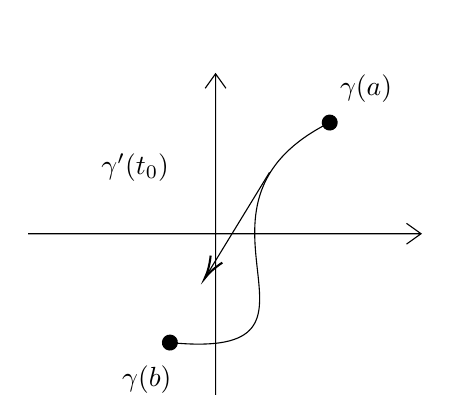
\begin{tikzpicture}[x=0.75pt,y=0.75pt,yscale=-1,xscale=1]
        %uncomment if require: \path (0,286); %set diagram left start at 0, and has height of 286
        
        %Shape: Axis 2D [id:dp5992461788507699] 
        \draw  (50,141.08) -- (239.26,141.08)(140.26,64) -- (140.26,226.51) (232.26,136.08) -- (239.26,141.08) -- (232.26,146.08) (135.26,71) -- (140.26,64) -- (145.26,71)  ;
        %Curve Lines [id:da8169369769076535] 
        \draw    (118.26,193.51) .. controls (210.26,202.51) and (113.26,128.51) .. (195.26,87.51) ;
        \draw [shift={(195.26,87.51)}, rotate = 333.43] [color=black  ][fill=black  ][line width=0.75]      (0, 0) circle [x radius= 3.35, y radius= 3.35]   ;
        \draw [shift={(118.26,193.51)}, rotate = 5.59] [color=black  ][fill=black  ][line width=0.75]      (0, 0) circle [x radius= 3.35, y radius= 3.35]   ;
        %Straight Lines [id:da7279313778056917] 
        \draw    (166.26,111.51) -- (136.05,160.92) ;
        \draw [shift={(135,162.63)}, rotate = 301.44] [color=black  ][line width=0.75]    (10.93,-3.29) .. controls (6.95,-1.4) and (3.31,-0.3) .. (0,0) .. controls (3.31,0.3) and (6.95,1.4) .. (10.93,3.29)   ;
        
        % Text Node
        \draw (199,63.4) node [anchor=north west][inner sep=0.75pt]    {$\gamma ( a)$};
        % Text Node
        \draw (94,203.4) node [anchor=north west][inner sep=0.75pt]    {$\gamma ( b)$};
        % Text Node
        \draw (84,101.4) node [anchor=north west][inner sep=0.75pt]    {$\gamma '( t_{0})$};
        
        
        \end{tikzpicture}
\]

\defn Parameterize $\gamma(t)=(x(t), y(t))=x(t)+iy(t)$. Then $\gamma'(t_0)=(x'(t_0), y'(t_0))$ is a \textbf{tangent vector} to the curve at $\gamma(t_0)$ (assume $\gamma'(t_0)\neq \mathbf{0}$, aka. $\gamma$ is regular at $\gamma(t_0)$.)

\begin{theorem}[The ``Boxy-path'' Theorem]
    A nonempty open set $\Omega$ in $\C$ is connected \textit{if and only if} each pair of distinct
points in $\Omega$ can be joined by a sequence of line segments lying in $\Omega$, each of which is
parallel to either to the real or imaginary axis.
    \drawing{0.6\linewidth}{image-3.png}
    In other words, between any 2 points in a region $\reg$ there exists a ``\textbf{boxy path}''.
\end{theorem}

\rmk There is also always a \textbf{smooth path}. That is: \drawing{150pt}{image-4.png}

\begin{theorem}[``Smooth-path'']
    A nonempty open set $\reg$ in $\C$ is connected if and only if each pair of distinct
points in $\reg$ can be joined by a continuously differentiable curve in $\reg$ that is regular at
every point.
\end{theorem}
\begin{proof}
    See \href{https://stephangarcia.sites.pomona.edu/teaching/24S-135/Lecture/24S-135-Lecture02.pdf}{lecture 2 notes}.
\end{proof}

\subsection{Conformality}
Let $f$ be an analytic complex function on $\reg$.

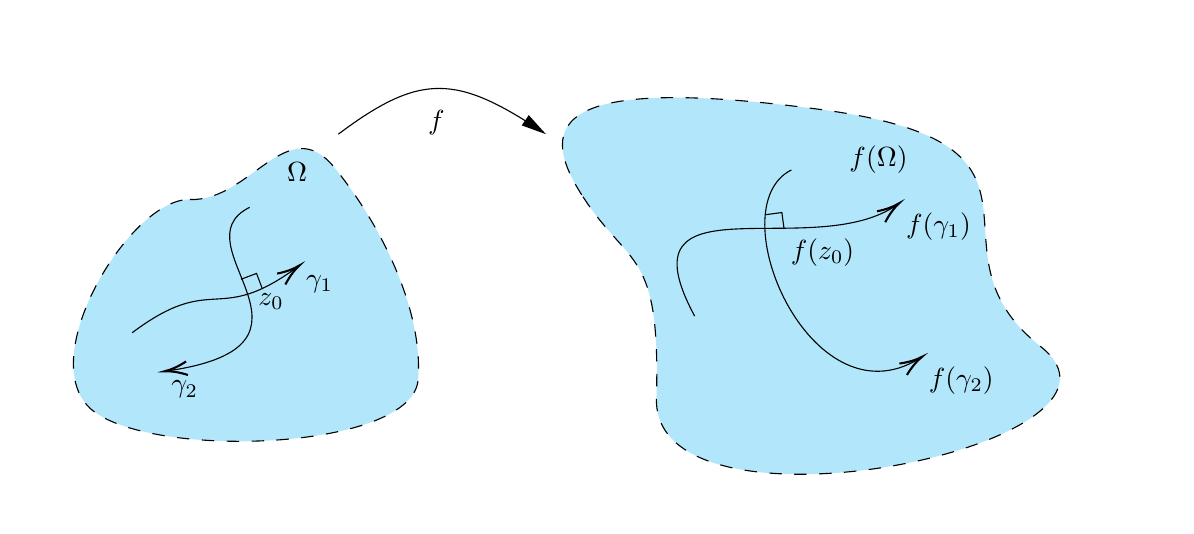
\begin{tikzpicture}[x=0.75pt,y=0.75pt,yscale=-1,xscale=1]
    %uncomment if require: \path (0,300); %set diagram left start at 0, and has height of 300
    
    %Shape: Polygon Curved [id:ds04152892949921583] 
    \draw  [fill=cyan  ,fill opacity=0.3 ][dash pattern={on 4.5pt off 4.5pt}] (92.5,102.5) .. controls (121.5,103.5) and (139.5,59.5) .. (162,87) .. controls (184.5,114.5) and (204.91,155.75) .. (202.42,189.25) .. controls (199.92,222.75) and (79.59,227.75) .. (47.08,205.25) .. controls (14.58,182.75) and (63.5,101.5) .. (92.5,102.5) -- cycle ;
    %Curve Lines [id:da38490573070321243] 
    \draw    (64.67,166.67) .. controls (104.27,136.97) and (105.24,163.7) .. (144.07,135.13) ;
    \draw [shift={(145.25,134.25)}, rotate = 143.13] [color=black  ][line width=0.75]    (10.93,-3.29) .. controls (6.95,-1.4) and (3.31,-0.3) .. (0,0) .. controls (3.31,0.3) and (6.95,1.4) .. (10.93,3.29)   ;
    %Curve Lines [id:da9683797356751562] 
    \draw    (121.25,106.25) .. controls (85.43,124.16) and (167.43,172.76) .. (81.56,185.07) ;
    \draw [shift={(80.25,185.25)}, rotate = 352.23] [color=black  ][line width=0.75]    (10.93,-3.29) .. controls (6.95,-1.4) and (3.31,-0.3) .. (0,0) .. controls (3.31,0.3) and (6.95,1.4) .. (10.93,3.29)   ;
    %Shape: Right Angle [id:dp0014762610750393979] 
    \draw   (117.1,140.91) -- (124.59,138.1) -- (127.4,145.59) ;
    %Shape: Polygon Curved [id:ds020760136591730705] 
    \draw  [fill=cyan  ,fill opacity=0.3 ][dash pattern={on 4.5pt off 4.5pt}] (281.25,100.25) .. controls (258.25,64.25) and (271.25,42.25) .. (397.25,59.25) .. controls (523.25,76.25) and (442.25,126.25) .. (502.25,173.25) .. controls (562.25,220.25) and (315.25,271.25) .. (317.25,198.25) .. controls (319.25,125.25) and (304.25,136.25) .. (281.25,100.25) -- cycle ;
    %Curve Lines [id:da5067199553805877] 
    \draw    (335.67,158.67) .. controls (298.63,89.94) and (392.35,133.36) .. (433.04,105.13) ;
    \draw [shift={(434.25,104.25)}, rotate = 143.13] [color=black  ][line width=0.75]    (10.93,-3.29) .. controls (6.95,-1.4) and (3.31,-0.3) .. (0,0) .. controls (3.31,0.3) and (6.95,1.4) .. (10.93,3.29)   ;
    %Curve Lines [id:da12902529814050778] 
    \draw    (382.25,88.25) .. controls (346.61,106.07) and (391.34,211.12) .. (443.67,179.26) ;
    \draw [shift={(445.25,178.25)}, rotate = 146.56] [color=black  ][line width=0.75]    (10.93,-3.29) .. controls (6.95,-1.4) and (3.31,-0.3) .. (0,0) .. controls (3.31,0.3) and (6.95,1.4) .. (10.93,3.29)   ;
    %Shape: Right Angle [id:dp16473621622546486] 
    \draw   (369.76,109.81) -- (377.69,108.76) -- (378.75,116.69) ;
    %Curve Lines [id:da7241992906101147] 
    \draw    (164,71) .. controls (203.6,41.3) and (220.91,42.23) .. (262.73,70.15) ;
    \draw [shift={(264,71)}, rotate = 213.92] [fill=black  ][line width=0.08]  [draw opacity=0] (12,-3) -- (0,0) -- (12,3) -- cycle    ;
    
    % Text Node
    \draw (138,83.4) node [anchor=north west][inner sep=0.75pt]    {$\Omega $};
    % Text Node
    \draw (147.25,137.65) node [anchor=north west][inner sep=0.75pt]    {$\gamma _{1}$};
    % Text Node
    \draw (82.25,188.65) node [anchor=north west][inner sep=0.75pt]    {$\gamma _{2}$};
    % Text Node
    \draw (124.25,146.65) node [anchor=north west][inner sep=0.75pt]    {$z_{0}$};
    % Text Node
    \draw (409,75.4) node [anchor=north west][inner sep=0.75pt]    {$f( \Omega )$};
    % Text Node
    \draw (436.25,107.65) node [anchor=north west][inner sep=0.75pt]    {$f( \gamma _{1})$};
    % Text Node
    \draw (447.25,181.65) node [anchor=north west][inner sep=0.75pt]    {$f( \gamma _{2})$};
    % Text Node
    \draw (380.75,120.09) node [anchor=north west][inner sep=0.75pt]    {$f( z_{0})$};
    % Text Node
    \draw (206,58.4) node [anchor=north west][inner sep=0.75pt]    {$f$};
    
    
\end{tikzpicture}

Let $z_0\in \reg$ such that $f'(z_0)\neq 0$. Let $\gamma_1, \gamma_2$ be two curves that pass through $z_0$ intersecting with an angle $\theta$. Then $f(\gamma_1), f(\gamma_2)$ are two curves in $f(\Omega)$ passing through $f(\zeta_0)$ also with angle $\theta$.

Therefore, $f$ is \textbf{conformal}!

\section{Cauchy-Riemann equations, harmonic functions}
\subsection{Multivariate notion of complex derivatives}
Recall: $\displaystyle f'(z_0)=\lim_{h\to 0}\frac{f(z_0+h)-f(z_0)}{h}$.

Now we write each function with complex variables as $f(z)=u(z)+i\, v(z)$ where $u,v$ are real-valued \sidenote{meaning their range is real} functions.

Since $\C\cong \R^2$, we denote every point $z=(x,y)$.

Now we let $f(x,y)=u(x,y)+i\,v(x,y)$. We first let the small distance $h=(r,0)$ be horizontally approaching 0 with $r\in \R$. That is, $z_0+h=(x_0+r,y_0)$.
\begin{align*}
    f'(z_0) &= \lim_{r\to 0} \frac{u(x_0+r, y_0)-u(x_0,y_0)}{r} + i\cdot \lim_{r\to 0}\frac{v(x_0+r, y_0)-v(x_0,y_0)}{r}\\
    &=u_x(x_0,y_0)+i\cdot v_x(x_0,y_0)
\end{align*}

Similarly, if we vertically let $h=ir=(0,r)$ with $r\to 0, r\in \R$, we would get $f'=v_y-i\cdot u_y$.

\rmk If a derivative exists, the horizontal \& the vertical ones should be equal!

\begin{theorem}[Cauchy-Riemann Equations]
    \begin{align*}
        u_x &=v_y\\
        u_y &= -v_x
    \end{align*}
\end{theorem}\addlink{Cauchy-Riemann Equations}

\begin{corollary}
    If $f:\reg \to \C$ is analytic and $f'=0$ on $\reg$, then $f$ is \textbf{constant}.
\end{corollary}
\begin{proof}
    Since $0=f'=u_x+iv_x$, we see that $u_x=v_x=0$ on $\reg$. By Cauchy-Riemann, $v_y=u_y=0$ is also true on $\reg$. Hence, $\mathbf{u}, \mathbf{v}$ are constant on either horizontal or vertical segments. By the Boxy Path Theorem, $f=u+iv$ cannot assume two distinct values in $\reg$.
\end{proof}

\subsection{Orientation-preserving as shown by Jacobian}
Let $f:\reg \to \C$ be analytic. Then $f'=u_x+iv_x$ and hence:\begin{align*}
    |f'|^2 = \bar f'\cdot f &= (u_x-iv_x)(u_x+iv_x)\\
    &= u_x^2 + v_x^2\\
    &= u_xu_x+v_xv_x && \text{and by Cauchy-Riemann,}\\
    &= u_xv_y-u_yv_x\\
    &= \det\left(\begin{bmatrix}
        u_x & u_y\\
        v_x & v_y
    \end{bmatrix}\right) && \text{the Jacobian of $f$!}
\end{align*}

Since $|f'|^2\geq 0$, the determinant of the Jacobian is always $\geq 0$, implying that $f$ is always locally orientation-preserving. Moreover,

\begin{proposition}
    If $f'(z_0)\neq 0$, then $|f'|^2> 0$ implies:
    \begin{enumerate}
        \item $f$ is \textbf{injective} near $z_0$
        \item $f$ scales $\R$ by $|f'(z_0)|^2$ near $z_0$
        \item $f$ preserves orientation near $z_0$
    \end{enumerate}
\end{proposition}

\subsection{The Laplacian, harmonic functions and conjugates}
Suppose that $f=u+iv$ is analytic and $u,v$ have continuous second partial derivatives. Then:\begin{align*}
    u_{xx}+u_{yy} = \Delta u = (v_y)_x + (-v_x)_y = v_{yx}-v_{xy}=0
\end{align*}
This means that the Laplacian of this function $u$ is 0!\sidenote{$\Delta u = 0$ characterizes steady-state solutions to heat equations on $\reg$.}

\defn Real-valued functions $u: \reg\to \R$ satisfying that the Laplacian $\Delta u= u_{xx}+u_{yy}$ is 0 on $\reg$ is called \textbf{harmonic functions}.

\defn A \textbf{harmonic conjugate} of $u$ is a harmonic function $v: \reg \to \R$ such that $f=u+i\cdot v$ is \textbf{analytic} on $\reg$.
\addlink{Harmonic conjugate}

\eg $u=x^2-y^2, v=2xy$.\sidenote{Check it!}

\rmk Harmonic conjugates are unique up to translation (± constants).

\rmk If $u$ is harmonic on $\reg$, it does NOT have to have a harmonic conjugate on $\reg$.

\subsection{Finding a harmonic conjugate}
Recall that the real and imaginary parts of an analytic function are \textbf{harmonic}, in addition to satisfying the Cauchy-Riemann Equations: $u_x=v_y$ and $u_y=-v_x$.

\eg $u(z)=\log |z|$ is harmonic on $\C\backslash\{0\}$.
\begin{proof}
    Write $u(x,y)=\log (\sqrt{x^2+y^2})=\frac{1}{2}\log(x^2+y^2)$.

    Then, \begin{align*}
        u_x&=\frac{\partial}{\partial x}\left(\frac{1}{2}\log (x^2+y^2)\right)\\
        &= \frac{1}{2}\cdot \frac{2x}{x^2+y^2}\\
        &= \frac{x}{x^2+y^2}
    \end{align*}

    Hence,\sidenote{Review quotient rule!}
    \begin{align*}
        u_{xx} &= \frac{(x^2+y^2)-x(2x)}{(x^2+y^2)^2}\\
        &= \frac{y^2-x^2}{(x^2+y^2)^2}
    \end{align*}

    Symmetrically, we find \begin{align*}
        u_{yy} & = \frac{x^2-y^2}{(x^2+y^2)^2}
    \end{align*}
    Hence $u_{xx}+u_{yy}=0$, implying that the function is harmonic.
\end{proof}

Now, can we \uline{find a harmonic conjugate for the aforementioned $u$}?\sidenote{There is currently a great \textbf{CAVEAT} in all of these, because $v(z)=\arg(z)$ cannot be defined in a continuous manner in all of $\C\backslash\{0\}$: 

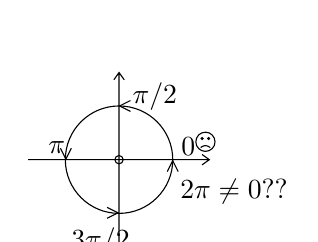
\begin{tikzpicture}[x=0.75pt,y=0.75pt,yscale=-0.5,xscale=0.5]
    %uncomment if require: \path (0,300); %set diagram left start at 0, and has height of 300
    
    %Shape: Axis 2D [id:dp48156480156165227] 
    \draw  (111,139) -- (285.5,139)(198.5,55) -- (198.5,219) (278.5,134) -- (285.5,139) -- (278.5,144) (193.5,62) -- (198.5,55) -- (203.5,62)  ;
    %Shape: Circle [id:dp6012967995903811] 
    \draw   (146.75,139) .. controls (146.75,110.42) and (169.92,87.25) .. (198.5,87.25) .. controls (227.09,87.25) and (250.26,110.42) .. (250.26,139) .. controls (250.26,167.58) and (227.09,190.75) .. (198.5,190.75) .. controls (169.92,190.75) and (146.75,167.58) .. (146.75,139) -- cycle ;
    \draw   (209.5,92.5) -- (199,87.25) -- (209.5,82) ;
    \draw   (152.5,128) -- (147.25,138.5) -- (142,128) ;
    \draw   (187,185) -- (197.5,190.25) -- (187,195.5) ;
    \draw   (245,150.5) -- (250.25,140) -- (255.5,150.5) ;
    %Shape: Smiley Face [id:dp013237994815757492] 
    \draw   (272.5,121.75) .. controls (272.5,116.64) and (276.64,112.5) .. (281.75,112.5) .. controls (286.86,112.5) and (291,116.64) .. (291,121.75) .. controls (291,126.86) and (286.86,131) .. (281.75,131) .. controls (276.64,131) and (272.5,126.86) .. (272.5,121.75) -- cycle ; \draw   (277.68,118.61) .. controls (277.68,118.09) and (278.09,117.68) .. (278.61,117.68) .. controls (279.12,117.68) and (279.53,118.09) .. (279.53,118.61) .. controls (279.53,119.12) and (279.12,119.53) .. (278.61,119.53) .. controls (278.09,119.53) and (277.68,119.12) .. (277.68,118.61) -- cycle ; \draw   (283.97,118.61) .. controls (283.97,118.09) and (284.38,117.68) .. (284.9,117.68) .. controls (285.41,117.68) and (285.82,118.09) .. (285.82,118.61) .. controls (285.82,119.12) and (285.41,119.53) .. (284.9,119.53) .. controls (284.38,119.53) and (283.97,119.12) .. (283.97,118.61) -- cycle ; \draw   (277.13,127.3) .. controls (280.21,124.83) and (283.29,124.83) .. (286.38,127.3) ;
    %Shape: Circle [id:dp5943162664556252] 
    \draw   (194.51,139) .. controls (194.51,136.79) and (196.3,135) .. (198.5,135) .. controls (200.71,135) and (202.5,136.79) .. (202.5,139) .. controls (202.5,141.21) and (200.71,143) .. (198.5,143) .. controls (196.3,143) and (194.51,141.21) .. (194.51,139) -- cycle ;
    
    % Text Node
    \draw (256,115.4) node [anchor=north west][inner sep=0.75pt]    {$0$};
    % Text Node
    \draw (209,62.4) node [anchor=north west][inner sep=0.75pt]    {$\pi /2$};
    % Text Node
    \draw (128,119.4) node [anchor=north west][inner sep=0.75pt]    {$\pi $};
    % Text Node
    \draw (150,202.4) node [anchor=north west][inner sep=0.75pt]    {$3\pi /2$};
    % Text Node
    \draw (255,155.4) node [anchor=north west][inner sep=0.75pt]    {$2\pi \neq 0??$};
    
    
    \end{tikzpicture}
    

To be resolved later!}

We could use the two Cauchy-Riemann Equations. One of them:
\begin{align*}
    v_y&=u_x\\
    &= \frac{x}{x^2+y^2}
\end{align*}
Therefore, \begin{align*}
    v(x,y) &= \int v_ydy + C(x) && \text{unknown function of }x\\
    &= \arctan\left(\frac{y}{x}\right)+C(x)
\end{align*}

Then, we use the second one: \begin{align*}
    \frac{y}{x^2+y^2}=u_y=-v_x &= -\frac{\partial}{\partial x} \left( \arctan\left(\frac{y}{x}\right)+C(x)\right)\\
    &= \frac{y}{x^2+y^2}-C'(x) \implies C'(x)=0
\end{align*}

Hence, a good harmonic conjugate candidate seems to be \begin{align*}
    v(x,y) = \arctan\left(\frac{y}{x}\right) + C
\end{align*}
where $C$ is a constant. WLOG, let $C=0$. Then $ v(x,y)=\arctan\left(\frac{y}{x}\right)$, meaning that: \begin{align*}
    v(z)=\arg (z)
\end{align*}

Therefore, $f(z)=\log |z| + i\cdot \arg(z)$ is analytic!
%%%%%%%

\subsection{Physics analogies of harmonic functions}
\eg Let $T(x,y,t)$ be the temperature at $(x,y)$ at time $t$ of a thermally conductive plate in $\C$. Assume the plate gives rise to a \textbf{bounded} region $\Omega$ (with boundary denoted $\partial \Omega$). Temperature on $\partial \Omega$ is a fixed function (time-independent).

\begin{figure}[H]
    \centering
    
\includegraphics[width=80pt]{Images/image-2.png}
\end{figure}

Now given the heat equation: \begin{align*}
    \frac{\partial T}{\partial t}-\alpha \Delta T=0
\end{align*}
where $\alpha$ is a constant.

We think the system tends towards a thermal equilibrium as $t\to \infty$. At equilibrium, $\frac{\partial T}{\partial t}$ is \textbf{zero}. Hence, at equilibrium, $\Delta T=T_{xx}+T_{yy}=0$.

\textbf{\underline{Idea}}: \hypertarget{physics}{Harmonic function behave like equilibrium temperature distributions!}

\begin{proposition}
    Let $U(x,y)$ be a harmonic function on $\Omega$.
    \begin{enumerate}
        \item $U$ cannot have a \textit{local} maximum in $\Omega$.
        \item The absolute maximum of $U$ on $\Omega ^-$\sidenote{$\Omega ^-$ denotes the closure of $\Omega$} occurs on $\partial \Omega$.
        \item $U$ cannot be locally constant without being globally constant.
    \end{enumerate}
\end{proposition}

\begin{theorem}[Maximum principle]
    Let $\Omega$ be a bounded region in $\C$ and let $f: \Omega^-\to \C$ be analytic on $\Omega$ and continuous on $\Omega^-$.
    \begin{enumerate}
        \item If $|f|$ achieves a local max in $\Omega$, then $f$ is constant.
        \item The global max of $|f|$ on $\Omega^-$ is attained on $\partial \Omega$.
    \end{enumerate}
\end{theorem}

\section{Möbius transformations}
\subsection{Möbius transformations, the extended plane}
\defn[Möbius transformations]
\begin{align*}
    f(z)=\frac{az+b}{cz+d}\text{ where } ad-bc\neq 0, a,b,c,d\in \C
\end{align*}
Such an $f$ is \textbf{analytic} on $\C\backslash\{\frac{-d}{c}\}$\sidenote{recall that rational functions are analytic except when the denominator vanishes, i.e. $cz+d\neq 0$.} and \textbf{comformal} there since $f'(z)=\frac{ad-bc}{(cz+d)^2}\neq 0$ on $\C\backslash\{\frac{-d}{c}\}$.

\rmk In addition, $f$ is injective (one-to-one)!
\begin{proof}
    \begin{align*}
        f(z)=f(w)\implies \frac{az+b}{cz+d}&=\frac{aw+b}{cw+d}\\
         (az+b)(cw+d)&= (cz+d)(aw+b)\\
         aczw+bcw+a\d z+bd&=aczw+adw+bcz+bd\\
         (ad-bc)z&=(ad-bc)w\\
         z&=w
    \end{align*}
\end{proof}

\defn[The extended plane] We set the following convention:\begin{align*}
    f(\frac{-d}{c})&= \infty\\
    f(\infty) &= \frac{a}{c}
\end{align*}
with this, $f$ is a \textbf{bijection} from $\Chat=\C\cup\{\infty\}$ to itself.\sidenote{recall Riemann sphere}

\subsection{Möbius transformations as matrices}
\rmk We can \textit{associate}\sidenote{this association is not a bijection: it's only so up to scaling} $f(z)=\frac{az+b}{cz+d}$ where $ad-bc\neq 0$ with the matrix $$M_f=\begin{bmatrix}
    a&b\\c&d
\end{bmatrix}$$

\rmk $M_{f\circ g}=M_f\cdot M_g$\sidenote{check this!}

\rmk The inverse of $M_f=\begin{bmatrix}
    a&b\\c&d
\end{bmatrix}$ is $M_f^{-1}=\frac{1}{ad-bc}\begin{bmatrix}
    d&-b\\-c&a
\end{bmatrix}$ and scaling does not matter, so we could write the \textbf{inverse} of such Möbius transformation as: \begin{align*}
    \inv{f}(w) &=\frac{dw-b}{-cw+a}
\end{align*}

\begin{theorem}
    A Möbius transformation $f:\Chat\to\Chat$ with three fixed points in $\Chat$ is the \textbf{identity map} $\mathrm{id}(z)=z=\frac{z+0}{0z+1}$.\sidenote{$I=\begin{bmatrix}
        1&0\\0&1
    \end{bmatrix}$}
\end{theorem}
\begin{proof}
    Let $f(z)=\frac{az+b}{cz+d}$ be a Möbius transformation.
    \begin{enumerate}
        \item If $\infty$ is fixed, then $c=0$\sidenote{think about that!}. Then $f(z)=\frac{a}{d}z+\frac{b}{d}$, which is a \textbf{linear} transformation.\begin{enumerate}
            \item If $f(z)=z$, we are done since we get the identity!
            \item Otherwise the function only has one fixed point at $\infty$.
        \end{enumerate}
        \item If $\infty$ is not a fixed point, then $c\neq 0$. Solve:\begin{align*}
            f(z)+z \Leftrightarrow \frac{az+b}{cz+d}&=z\\
            az+b&=cz^2+\d z\\
            cz^2+(d-a)z-b&=0
        \end{align*}
        is a quadratic which has at most two (distinct) solutions in $\C$. Hence, this transformation fixes at most two points.
    \end{enumerate}
\end{proof}

\subsection{Möbius transformations take circles to circles}
\rmk Lines can be circles (they are just circles that pass through the point at infinity).

\begin{theorem}
    The image of a circle under a Möbius transformation is still a circle.
\end{theorem}
\begin{proof}
    Let $f(z)=\frac{az+b}{cz+d}$ be a Möbius transformation.
    \begin{enumerate}
        \item If $c=0$, then $f(z)=\frac{a}{d}z+\frac{b}{d}$, which is a \textbf{linear/affine} transformation and so we are done\sidenote{since linear transformations preserve circles and lines}.
        \item Now suppose $c\neq 0$. Then \begin{align*}
            f(z)&=\frac{a}{d}z+\frac{b}{d}\\
            &= \frac{\frac{a}{c}(cz+d)-\frac{ad}{c}+b}{cz+d}\\
            &= \frac{b-\frac{ad}{c}}{cz+d}+\frac{a}{c}
        \end{align*}
        which is a composition of affine, inversion and affine:
        $$z\mapsto cz+d\mapsto \frac{1}{cz+d}\mapsto \frac{b-\frac{ad}{c}}{cz+d}+\frac{a}{c}$$
        We now only need to show that inversion preserves circles.

        Let a circle in $\R^2$ be $Ax+By+C(x^2+y^2)=D$ where $A,B,C,D\in \R$. If $z=x+iy\in \Chat$, then $\frac{1}{z}=\frac{x}{x^2+y^2}+i\frac{-y}{x^2+y^2}$. Name $\frac{1}{z}=u+iv$, note that $u^2+v^2=\frac{1}{x^2+y^2}$. 
        
        Then we note that $Au-Bv+C=D(u^2+v^2)$\sidenote{check this!}, which is still a circle!
    \end{enumerate}
\end{proof}

\begin{theorem}
    Given two triples $z_1,z_2,z_3$ and $w_1,w_2,w_3$ of \textit{distinct} points in $\Chat$, then there is always a unique Möbius transformation $f$ such that $f(z_i)=w_i$ for all $i=1,2,3$.
\end{theorem}
\begin{proof}
    Claim: the \textit{cross-ratio} $\phi(z)=\frac{z-z_1}{z-z_3}\cdot \underset{\text{const.}}{\underbrace{\frac{z_2-z_3}{z_2-z_1}}}$ is a Möbius transformation that satisfies \circled{$\phi(z_1)=0, \phi(z_2)=1, \phi(z_3)=\infty$}.

    We can also find another Möbius transformation such that $\psi(z_1)=0, \psi(z_2)=1, \psi(z_3)=\infty$. Then:
    \[\begin{tikzcd}[ampersand replacement=\&,cramped,row sep=tiny]
        {z_1} \& 0 \& {w_1} \\
        {z_2} \& 1 \& {w_2} \\
        {z_3} \& \infty \& {w_3}
        \arrow["\phi", maps to, from=1-1, to=1-2]
        \arrow["{\psi^{-1}}", maps to, from=1-2, to=1-3]
        \arrow["\phi", maps to, from=2-1, to=2-2]
        \arrow["{\psi^{-1}}", maps to, from=2-2, to=2-3]
        \arrow["\phi", maps to, from=3-1, to=3-2]
        \arrow["{\psi^{-1}}", maps to, from=3-2, to=3-3]
    \end{tikzcd}\]

    and we could simply let $f=\psi^{-1}\circ \phi$.
\end{proof}

\eg Let $f(z)=\frac{z+1}{-z+1}$. We compute:\begin{align*}
    f(0)&=1\\
    f(-1)&=0\\
    f(1)&=\infty\\
    f(i)&=i\\
    f(-i)&=-i\\
\end{align*}

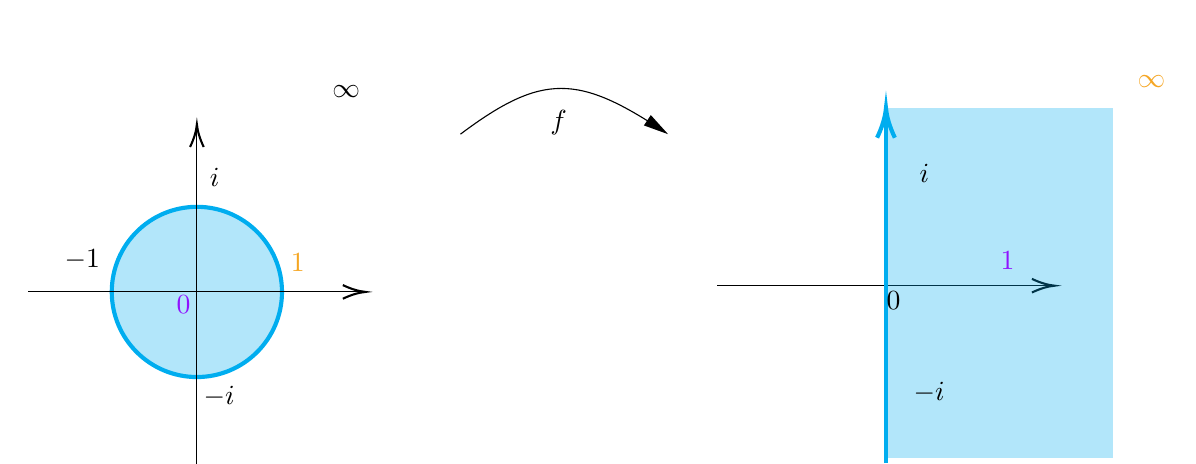
\begin{tikzpicture}[x=0.75pt,y=0.75pt,yscale=-1,xscale=1]
%uncomment if require: \path (0,300); %set diagram left start at 0, and has height of 300

%Shape: Circle [id:dp46487660565461075] 
\draw  [color=cyan  ,draw opacity=1 ][fill=cyan  ,fill opacity=0.3 ][line width=1.5]  (96,156.01) .. controls (96,133.37) and (114.36,115.01) .. (137.01,115.01) .. controls (159.65,115.01) and (178.01,133.37) .. (178.01,156.01) .. controls (178.01,178.66) and (159.65,197.02) .. (137.01,197.02) .. controls (114.36,197.02) and (96,178.66) .. (96,156.01) -- cycle ;
%Curve Lines [id:da6037660096213038] 
\draw    (264,80) .. controls (303.6,50.3) and (320.91,51.23) .. (362.73,79.15) ;
\draw [shift={(364,80)}, rotate = 213.92] [fill=black  ][line width=0.08]  [draw opacity=0] (12,-3) -- (0,0) -- (12,3) -- cycle    ;
%Straight Lines [id:da30485423184171] 
\draw    (55.75,156.01) -- (216.26,156.01) ;
\draw [shift={(218.26,156.01)}, rotate = 180] [color=black  ][line width=0.75]    (10.93,-3.29) .. controls (6.95,-1.4) and (3.31,-0.3) .. (0,0) .. controls (3.31,0.3) and (6.95,1.4) .. (10.93,3.29)   ;
%Straight Lines [id:da03496103337291223] 
\draw    (387.75,153.01) -- (548.26,153.01) ;
\draw [shift={(550.26,153.01)}, rotate = 180] [color=black  ][line width=0.75]    (10.93,-3.29) .. controls (6.95,-1.4) and (3.31,-0.3) .. (0,0) .. controls (3.31,0.3) and (6.95,1.4) .. (10.93,3.29)   ;
%Straight Lines [id:da11880027193931353] 
\draw    (137.01,246.26) -- (137.01,77.26) ;
\draw [shift={(137.01,75.26)}, rotate = 90] [color=black  ][line width=0.75]    (10.93,-3.29) .. controls (6.95,-1.4) and (3.31,-0.3) .. (0,0) .. controls (3.31,0.3) and (6.95,1.4) .. (10.93,3.29)   ;
%Straight Lines [id:da4256972022746721] 
\draw [color=cyan  ,draw opacity=1 ][line width=1.5]    (469.01,238.51) -- (469.01,70.51) ;
\draw [shift={(469.01,67.51)}, rotate = 90] [color=cyan  ,draw opacity=1 ][line width=1.5]    (14.21,-4.28) .. controls (9.04,-1.82) and (4.3,-0.39) .. (0,0) .. controls (4.3,0.39) and (9.04,1.82) .. (14.21,4.28)   ;
%Shape: Rectangle [id:dp17327106892852906] 
\draw  [draw opacity=0][fill=cyan  ,fill opacity=0.3 ] (469.01,67.51) -- (578.26,67.51) -- (578.26,236.26) -- (469.01,236.26) -- cycle ;

% Text Node
\draw (142,95.4) node [anchor=north west][inner sep=0.75pt]    {$i$};
% Text Node
\draw (181,136.4) node [anchor=north west][inner sep=0.75pt]  [color={rgb, 255:red, 245; green, 166; blue, 35 }  ,opacity=1 ]  {$1$};
% Text Node
\draw (139.01,200.42) node [anchor=north west][inner sep=0.75pt]    {$-i$};
% Text Node
\draw (72,134.4) node [anchor=north west][inner sep=0.75pt]    {$-1$};
% Text Node
\draw (126,156.4) node [anchor=north west][inner sep=0.75pt]  [color={rgb, 255:red, 144; green, 19; blue, 254 }  ,opacity=1 ]  {$0$};
% Text Node
\draw (484,93.4) node [anchor=north west][inner sep=0.75pt]    {$i$};
% Text Node
\draw (523,135.4) node [anchor=north west][inner sep=0.75pt]  [color={rgb, 255:red, 144; green, 19; blue, 254 }  ,opacity=1 ]  {$1$};
% Text Node
\draw (481.01,198.42) node [anchor=north west][inner sep=0.75pt]    {$-i$};
% Text Node
\draw (468,154.4) node [anchor=north west][inner sep=0.75pt]    {$0$};
% Text Node
\draw (201,55.4) node [anchor=north west][inner sep=0.75pt]    {$\infty $};
% Text Node
\draw (306,67.4) node [anchor=north west][inner sep=0.75pt]    {$f$};
% Text Node
\draw (589,50.4) node [anchor=north west][inner sep=0.75pt]    {$\textcolor[rgb]{0.96,0.65,0.14}{\infty }$};


\end{tikzpicture}

\section{Recall: infinite series}
\defn $\sum_{n=1}^{\infty}a_n$ converges to $S$ if $\lim_{N\to \infty}S_N=S$ where $S_N=a_1+\dots+a_N$.\sidenote{$S_N$ is the $N$-th partial sum.}

\subsection{Divergence test}
\defn[Divergence test]A pair of contrapositives:\sidenote{Note it's not an \ifnif !}\begin{enumerate}
    \item If $\sum_{n=1}^{\infty}a_n$ converges, then $\lim_{n\to\infty}a_n=0$.
    \item If $\lim_{n\to\infty}a_n\neq 0$ (\textit{including the case where the limit doesn't exist}) then $\sum_{n=1}^{\infty}a_n$ diverges.
\end{enumerate}
\noneg The harmonic series $\sum_{n=1}^{\infty}\frac{1}{n}=1+\frac{1}{2}+\dots$ diverges\sidenote{diverges, but really \textbf{slowly}!} even though $a_n=\frac{1}{n}$ tends to 0 when $n$ tends to $\infty$.

\begin{theorem}
    If $\sum_{n=1}^{\infty}a_n$ converges, then $\lim_{N\to \infty}\sum_{n=N}^{\infty}a_n=\lim_{N\to \infty}S-S_N=0$.\sidenote{In other words, the tail of a convergent series goes to 0.}
\end{theorem}

\begin{theorem}[Cauchy Criterion]
    $\sum_{n=1}^{\infty}a_n$ converges \ifnif for all $\varepsilon>0$, there exists $N\in \N$ such that $k>j>N$ implies $\displaystyle \left|\sum_{n=j-1}^{k}a_n \right|=S_k-S_j<\varepsilon$.
\end{theorem}

\subsection{Integral test}

\defn[Integral test] Define $a_n=f(n)$ for $n\in \N$, where $f:[1,\infty[ \to \R$ is (piecewise) continuous, positive and decreasing. Then $\int_{1}^{\infty}f(x)\, \d x$ converges \ifnif $\sum_{n=1}^{\infty}a_n$ converges.\sidenote{do an improper integral!}

Moreover, $\int_{1}^{N}f(x)\,\d x\leq a_1+\dots+a_N\leq a_1+\int_{1}^{N}f(x)\,\d x$.

\eg Apply the above with $f(x)=\frac{1}{x}$.\sidenote{$a_n=\frac{1}{n}$} Then \begin{align*}
    \ln N\leq 1+\frac{1}{2}+\dots+\frac{1}{N}\leq 1+\ln N
\end{align*}
It is bounded below by a divergent function, so it must be divergent!

\begin{theorem}
    The ``$p$-series'' $\sum_{n=1}^{\infty}\frac{1}{n^p}$ converges \ifnif $p>1$.
\end{theorem}

\defn[Riemann zeta function] \begin{align*}
    \zeta(s)&=\sum_{n=1}^{\infty}\frac{1}{n^s} && \text{for Re}(s)>1
\end{align*}
\rmk Euler figured out: \begin{align*}
    \zeta(2)&=\frac{\pi^2}{6}\\
    \zeta(4)&=\frac{\pi^4}{90}\\
    \zeta(6)&=\frac{\pi^6}{945}\\
    \vdots
\end{align*}
\rmk R. Apéry showed that $\zeta(3)$ is irrational (1979)\sidenote{still an open question in mathematics}:
\[\zeta(3)=\sum_{n=1}^{\infty}\frac{1}{n^3}=1.202\dots\]
but no explicit formula known!

\subsection{Absolute convergence}

\defn A series $\sum_{n=1}^{\infty}a_n$ is:\begin{enumerate}
    \item \textbf{absolutely convergent} if $\sum_{n=1}^{\infty}|a_n|$ converges.\sidenote{Good}
    \item \textbf{conditionally convergent} if $\sum_{n=1}^{\infty}a_n$ converges but $\sum_{n=1}^{\infty}|a_n|$ diverges.\sidenote{BAD}
\end{enumerate}

\begin{theorem}
    Every absolutely convergent series converges.
\end{theorem}
\eg The alternating harmonic series\sidenote{Don't re-parenthesize the terms -- grouping would change the sequence and thus the partial sums!} $$\sum_{n=1}^{\infty}\frac{(-1)^{n+1}}{n}=1-\frac{1}{2}+\frac{1}{3}-\frac{1}{4}+\dots$$ converges to $\ln 2$. But the convergence is conditional because the absolute value $$\sum_{n=1}^{\infty}\left|\frac{(-1)^{n+1}}{n}\right|=\sum_{n=1}^{\infty}\frac{1}{n}$$ does not converge.

\begin{theorem}
    An absolutely convergent series may be rearranged without changing its value. That is, if $\phi:\N\to \N$ is a bijection, then\sidenote{This seems obvious for finite series, but consider how this is extraordinary for infinite series!} $$\sum_{n=1}^{\infty}a_n=\sum_{n=1}^{\infty}a_{\phi(n)}$$
\end{theorem}

\addlink{Riemann Rearrangement Theorem}
\begin{theorem}[Riemann Rearrangement Theorem]
    If $\sum_{n=1}^{\infty}a_n$ is a \uline{conditionally convergent} series of real numbers, then for \textbf{any} $S\in \R\cup \{-\infty,\infty\}$, there is a bijection $\phi:\N\to\N$ such that $\sum_{n=1}^{\infty}a_{\phi(n)}=S$.\sidenote{Meaning we can get it to be equal to whatever we want just by rearranging!}
\end{theorem}

\spl

Now if $\sum_{n=0}^{\infty}a_n$ and $\sum_{n=0}^{\infty}b_n$ converge, one might expect that \begin{align*}
    \left(\sum_{i=0}^{\infty}a_i\right)\left(\sum_{j=0}^{\infty}b_j\right)&=(a_0+a_1+\dots)(b_0+b_1+\dots)\\
    &= a_0b_0+(a_0b_1+a_1b_0)+\dots\\
    &= \sum_{n=0}^{\infty}c_n \text{ where } c_n=\sum_{k=0}^{n}a_kb_{n-k}
\end{align*}
But this only works if both series are absolutely convergent, in which case the new series is absolutely convergent.\sidenote{conditionally convergent doesn't work! See \href{https://stephangarcia.sites.pomona.edu/teaching/24S-135/Lecture/24S-135-Lecture06.pdf}{notes}.}

\subsection{Uniform convergence}
\defn A sequence of functions $f_n: X\to \C$ where $X\subseteq \C$ \textbf{converges uniformly} to $f:X\to \C$ if for all $\varepsilon>0$, there exists a $N\in \N$ such that $n\geq N$ implies $|f_n(z)-f(z)|<\varepsilon$ for all $z\in X$.\sidenote{This is MATH131!}
\drawing{0.6\linewidth}{image-5.png}

\addlink{Uniform convergence preserves continuity}
\begin{theorem}
    If $f_n: X\to \C$ are continuous and converges uniformly on $X$ to $f:X\to\C$, then $f$ is continuous on $X$.\sidenote{unif. conv. preserves continuity}
    In other words, the uniform limit of continuous functions is continuous.
\end{theorem}

\rmk $f_n$ converges to $f$ pointwise on $X$ if $\lim_{n\to \infty}f_n(z)=f(z)$ for all $z\in X$.\sidenote{This doesn't say anything about the rate each point converges.}
\drawing{0.6\linewidth}{image-6.png}

\addlink{Integrals work with uniform convergence}
\begin{theorem}
    If $f_n:[a,b]\to \C$ are continuous and converge uniformly on $[a,b]$ to $f$, then\sidenote{Integrals work with uniform convergence} $$
    \lim_{n\to \infty}\int_{a}^{b}f_n(x)\,\d x = \int_{a}^{b}f(x)\,\d x
    $$
\end{theorem}

\rmk Uniform convergence doesn't necessarily preserve differentiability, limit or derivatives!

\eg $f_n(x)=\sqrt{x^2+\frac{1}{n}}$ on $[-1,1]$ converges uniformly to $f_n(x)=|x|$. But the limit function is \textbf{not} differentiable at $x=0$ even though every $f_n$ were.

\begin{theorem}[Weierstrass $M$-Test] 
    Let $f_n:X\to \C$ satisfy $|f_n(z)|\leq M_n$ for all $z\in X$ and $n\in \N$. If $\sum_{n=1}^{\infty}M_n$ converges, then $\sum_{n=1}^{\infty}f_n(z)$ converges both \textbf{absolutely} and \textbf{uniformly} on $X$.
\end{theorem}

\section{Power series}
\defn A \textbf{power series} is a series of the form $\sum_{n=0}^{\infty}a_n(z-z_0)^n$. The $a_n$ is the \textit{coefficient} and $z_0$ is the \textit{center}.

\subsection{Convergence of geometric series}

\begin{theorem}
    The \textit{geometric series} ($a_n=1, z_0=0$) $\sum_{n=0}^{\infty}z^n$ converges absolutely to $\frac{1}{1-z}$ if $|z|<1$, and it diverges otherwise. 

    Moreover, for each $r\in [0,1[$, the convergence is \textbf{uniform} on $|z|\leq r$.
\end{theorem}
\begin{proof}
    If $|z|\geq 1$, then $z^n\not\to 0$, so by the test of divergence, the series diverges.

    Now suppose $|z|<1$. Then\sidenote{The fact that we can find a formula for this sum is quite rare! } \begin{align*}
        \sum_{n=0}^{\infty}z^n &= \lim_{N\to \infty}\sum_{n=0}^{N-1}z^n\\
        &= \lim_{N\to \infty}(1+z+z^2+\dots+z^{N-1})\\
        &= \lim_{N\to \infty}\frac{1-z^N}{1-z}\\
        &= \frac{1}{1-z} &\text{since }|z|<1
    \end{align*}
    Which gives us point-wise convergence. Then, for any $r$ such that $|z|\leq r<1$, we have \begin{align*}
        \sum_{n=0}^{\infty}|z^n|\leq \sum_{n=0}^{\infty}r^n =\frac{1}{1-r}<\infty
    \end{align*}
    Hence, by the Weierstrass $M$-test, the series converges \textit{absolutely and uniformly} on $|z|\leq r$.
\end{proof}

\rmk Moral of the story: \begin{itemize}
    \item The \textit{radius of convergence} $R=1$ has the property that the series converges on $|z|<R$, and diverges if $|z|>R$.
    
    \item The series converges \textit{uniformly} on $|z|\leq r<1$ but not on $|z|<1$ itself. Why?
    
    Let $r=1$; we need be able to get $N\in \N$ such that for all $n\geq N$, we have $\left|\frac{1-z^N}{1-z}-\frac{1}{1-z}\right|<1$ for all $|z|<1$. However, this is not gonna work: as $z\to 1$, observe that this is going to eventually exceed 1. 

    \item The limit function $\displaystyle \frac{1}{1-z}$ is \textbf{analytic} on $\C\backslash\{1\}$\sidenote{the limit function is well-defined way beyond the $\mathbb{D}$!}. But the geometric series represents this function \underline{only} on $|z|<1$. In a smaller set, the power series represents the function that might originally be defined on a much larger set. The limit function is the \textit{analytic continuation} of the series.
    
    \item The limit function $\displaystyle \frac{1}{1-z}$ is cool if $z\neq 1$\sidenote{in the complex number sense!}, but as long as $|z|=1$ (\textbf{even} if $z\neq 1$), the geometric series diverges!
\end{itemize}

\subsection{Radius of convergence}
\defn The \textbf{limit superior} ($\limsup$) of a sequence of nonnegative real numbers $x_n$ is the largest \textit{limit point}\sidenote{limits of a subsequence of $x_n$} of the $x_n$: $$\limsup_{n\to \infty}x_n=\inf_{n\geq 0}\sup_{m\geq n}x_m$$\sidenote{the RHS as in real analysis}\addlink{Limit superior}
If the sequence is unbounded, the $\limsup$ would be $\infty$.

\eg If $x_n$ is the sequence $0,1,0,1,\dots$ then $\displaystyle\limsup_{n\to \infty}x_n=1$.

\eg If $x_n$ is the sequence $0,1,0,\frac{1}{2}, 0, \frac{1}{3},\dots$, then $\displaystyle\limsup_{n\to \infty}x_n=0$.

\rmk If $x_n$ are nonnegative, then \begin{itemize}
    \item $\displaystyle \limsup_{n\to \infty}(a_n+b_n)=\limsup_{n\to \infty}a_n+\limsup_{n\to \infty}b_n$
    \item $\displaystyle \limsup_{n\to \infty}(a_nb_n)\leq (\limsup_{n\to \infty}a_n)(\limsup_{n\to \infty}b_n)$
\end{itemize}

\addlink{Cauchy-Hadamard formula}
\begin{theorem}[Cauchy-Hadamard]\hypertarget{cauchy-hadamard}{}
    Let $\sum_{n=0}^{\infty}a_n(z-z_0)^n$ be a power series. Define $R\in [0,\infty]$ by \sidenote{interpret $\frac{1}{0}=\infty$}\begin{align*}
        \frac{1}{R}=\limsup_{n\to \infty}\sqrt[n]{|a_n|}
    \end{align*}
    Then the $R$ is the \textit{radius of convergence}.
    \begin{enumerate}[label=(\alph*)]
        \item On $|z-z_0|<R$, the series converges \textbf{absolutely}.\sidenote{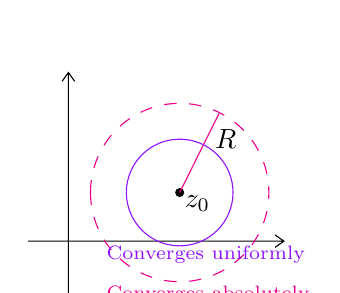
\begin{tikzpicture}[x=0.75pt,y=0.75pt,yscale=-0.6,xscale=.6]
            %uncomment if require: \path (0,300); %set diagram left start at 0, and has height of 300
            
            %Shape: Axis 2D [id:dp5858755410080565] 
            \draw  (50,212.68) -- (255.26,212.68)(82.26,77.28) -- (82.26,267.03) (248.26,207.68) -- (255.26,212.68) -- (248.26,217.68) (77.26,84.28) -- (82.26,77.28) -- (87.26,84.28)  ;
            %Shape: Circle [id:dp24544423482988642] 
            \draw  [color=magenta  ,draw opacity=1 ][dash pattern={on 4.5pt off 4.5pt}] (100,173.64) .. controls (100,134.09) and (132.06,102.03) .. (171.61,102.03) .. controls (211.17,102.03) and (243.23,134.09) .. (243.23,173.64) .. controls (243.23,213.19) and (211.17,245.26) .. (171.61,245.26) .. controls (132.06,245.26) and (100,213.19) .. (100,173.64) -- cycle ;
            %Shape: Circle [id:dp09425242443966897] 
            \draw  [fill=black  ,fill opacity=1 ] (168.46,173.64) .. controls (168.46,171.9) and (169.87,170.48) .. (171.61,170.48) .. controls (173.36,170.48) and (174.77,171.9) .. (174.77,173.64) .. controls (174.77,175.39) and (173.36,176.8) .. (171.61,176.8) .. controls (169.87,176.8) and (168.46,175.39) .. (168.46,173.64) -- cycle ;
            %Straight Lines [id:da3698233641764985] 
            \draw [color=magenta  ,draw opacity=1 ]   (203.26,110.07) -- (171.61,173.64) ;
            %Shape: Circle [id:dp40259923856296376] 
            \draw  [color={rgb, 255:red, 144; green, 19; blue, 254 }  ,draw opacity=1 ] (128.79,173.64) .. controls (128.79,149.99) and (147.96,130.81) .. (171.61,130.81) .. controls (195.27,130.81) and (214.44,149.99) .. (214.44,173.64) .. controls (214.44,197.29) and (195.27,216.47) .. (171.61,216.47) .. controls (147.96,216.47) and (128.79,197.29) .. (128.79,173.64) -- cycle ;
            
            % Text Node
            \draw (198,120.82) node [anchor=north west][inner sep=0.75pt]    {$R$};
            % Text Node
            \draw (173.61,173.88) node [anchor=north west][inner sep=0.75pt]    {$z_{0}$};
            % Text Node
            \draw (110.8,246.42) node [anchor=north west][inner sep=0.75pt]  [color=magenta  ,opacity=1 ] [align=left] {{\scriptsize Converges absolutely}};
            % Text Node
            \draw (110.8,214.62) node [anchor=north west][inner sep=0.75pt]   [align=left] {{\scriptsize \textcolor[rgb]{0.56,0.07,1}{Converges uniformly}}};
            
            
            \end{tikzpicture}} 
            For each $r\in [0,R[$, the convergence is \textbf{uniform} on $|z-z_0|\leq r$.        
        \item If $|z-z_0|>R$ then the series diverges. \rt{For $|z-z_0|=R$ anything could happen!}
    \end{enumerate}
\end{theorem}

\eg We claim that $\exp(z)=\sum_{n=0}^{\infty}\frac{z^n}{n!}$ has an infinite radius of convergence $R=\infty$. To check:
\begin{align*}
    \sqrt[n]{|a_n|} =\sqrt[n]{\frac{1}{n!}} = \frac{1}{\sqrt[n]{n!}}\to 0
\end{align*}
This is because $\sqrt[n]{n!} = \sqrt[n]{1\cdot 2\cdot\dots \cdot n}$, and in $n!$, there are at least $\frac{1}{2}$ terms that are $>\frac{n}{2}$. Thus, $\sqrt[n]{n!}\geq \left(\left(\frac{n}{2}\right)^{\frac{n}{2}}\right)^{\frac{1}{n}}=\left(\frac{n}{2}\right)^{1/2}\to \infty$.

So $R=\infty$ and we are done \begin{tikzpicture}[x=0.75pt,y=0.75pt,yscale=-.2,xscale=.2]%Shape: Smiley Face [id:dp9495597583093132] 
    \draw   (80,136) .. controls (80,116.67) and (95.67,101) .. (115,101) .. controls (134.33,101) and (150,116.67) .. (150,136) .. controls (150,155.33) and (134.33,171) .. (115,171) .. controls (95.67,171) and (80,155.33) .. (80,136) -- cycle ; \draw   (99.6,124.1) .. controls (99.6,122.17) and (101.17,120.6) .. (103.1,120.6) .. controls (105.03,120.6) and (106.6,122.17) .. (106.6,124.1) .. controls (106.6,126.03) and (105.03,127.6) .. (103.1,127.6) .. controls (101.17,127.6) and (99.6,126.03) .. (99.6,124.1) -- cycle ; \draw   (123.4,124.1) .. controls (123.4,122.17) and (124.97,120.6) .. (126.9,120.6) .. controls (128.83,120.6) and (130.4,122.17) .. (130.4,124.1) .. controls (130.4,126.03) and (128.83,127.6) .. (126.9,127.6) .. controls (124.97,127.6) and (123.4,126.03) .. (123.4,124.1) -- cycle ; \draw   (97.5,150) .. controls (109.17,159.33) and (120.83,159.33) .. (132.5,150) ;
    \end{tikzpicture}. We have that $\exp(z)$ has absolute convergence on the entire complex plane!

Absolute convergence means that we can multiply term-by-term:
\begin{align*}
    \exp(z)\exp(w) & = \left(\sum_{n=0}^{\infty}\frac{z^n}{n!}\right)\left(\sum_{n=0}^{\infty}\frac{w^n}{n!}\right)\\
    &= \sum_{n=0}^{\infty}\left(\sum_{k=0}^{\infty}\frac{z^k}{k!}\cdot\frac{w^{n-k}}{(n-k)!}\right)\\
    &= \sum_{n=0}^{\infty}\rt{\frac{1}{n!}}\underset{\text{binomial theorem}}{\underbrace{\sum_{k=0}^{\infty}\frac{\rt{n!}}{k!(n-k)!}z^kw^{n-k}}}\\
    &= \sum_{n=0}^{\infty}{\frac{1}{n!}}(z+w)^n\\
    &= \exp(z+w)
\end{align*}

Now define $e=\exp(1)=\sum_{n=0}^{\infty}\frac{1}{n!}$.

\subsection{Term-by-term differentiation of power series}

\begin{lemma}
    $n^{\frac{1}{n}}\to 1$
\end{lemma}
\begin{proof}[Proof 1] $e^{\log (n^{\frac{1}{n}})}=e^{\frac{\log n}{n}}\to e^{0}=1$ by l'Hopital. So $n^{\frac{1}{n}}\to 1$.
\end{proof}
\begin{proof}[Proof 2 (better)] Write $n^{\frac{1}{n}}=1+\delta_n$ where $\delta_n\geq 0$. The binomial theorem says:
\begin{align*}
    n&= (1+\delta_n)^n\\
    &= \sum_{k=0}^{\infty}{n\choose k}\delta_n^k\cdot 1^{n-k}\\
    &= 1+n\delta_n+\frac{n(n-1)}{2}\delta_n^2+\dots\\
    &\geq 1+\frac{n(n-1)}{2}\delta_n^2
\end{align*}
    Therefore, $n-1\geq \frac{n(n-1)}{2}\delta_n^2$ and we get $\frac{2}{n}\geq \delta_n^2\geq 0$ hence $\delta_n\to 0$.

    Hence $n^{\frac{1}{n}}\to 1$.
\end{proof}

\addlink{Derivative series have the same radius of convergence}
\begin{theorem}
    If $f(z)=\sum_{n=0}^{\infty}a_n(z-z_0)^{n}$ has radius of convergence $R$, then \[f'(z)=\sum_{n=0}^{\infty}na_n(z-z_0)^{n-1}\] for $|z-z_0|<R$. Moreover, the new series also has a radius of convergence $R$.
\end{theorem}
\begin{proof}
    WLOG $R>0$ and $z_0=0$\sidenote{we just translate it; also $R=0$ isn't that meaningful}. 
    
    For $|z|<R$ we write:\sidenote{just splitting the function into two parts}
    \[f(z)=\underset{S_N(z)}{\underbrace{\sum_{n=0}^{N-1}a_nz^n}} + \underset{R_N(z)}{\underbrace{ \sum_{n=N}^{\infty}a_nz^n}}\]
    and the `new series'\[g(z)=\sum_{n=0}^{\infty}na_nz^{n-1}=\lim_{N\to \infty}S'_N(z)\]

    We first prove that the radius of convergence for $g$ is the same as $f$. By Cauchy-Hadamard:
    \begin{align*}
        \frac{1}{R_g}&=\limsup_{n\to \infty}\sqrt[n]{n|a_n|}\\
        &=\limsup_{n\to \infty}(n^{\frac{1}{n}})\sqrt[n]{|a_n|} & \text{by the previous lemma,}\\
        &= \limsup_{n\to \infty}\sqrt[n]{|a_n|}\\
        &= \frac{1}{R}
    \end{align*}
    Thus, $R_g=R$ by Cauchy-Hadamard.

    Next, we need to show that $f'=g$ with $|z|<R$.

    Fix $0\leq |w|<R$ and $\varepsilon>0$. We want a $\delta>0$ such that whenever $|z-w|<\delta$,  we have $\left|\frac{f(z)-f(w)}{z-w}-g(w)\right|<\varepsilon$.\sidenote{just saying that the derivative at any $w$ gets close to $g(w)$}

    We rewrite:\begin{align*}
        \left|\frac{f(z)-f(w)}{z-w}-g(w)\right|
        &= \left| \frac{
            [S_N(z)+R_N(z)]-[S_N(w)+R_N(w)]
        }
        {z-w}
        -g(w)\right|\\
        &= \left|
            \frac{S_N(z)-S_N(w)}{z-w} +
            \frac{R_N(z)-R_N(w)}{z-w} +
            \gt{S'_N(w)-S'_N(w)} -
            g(w)
            \right|\\
        &\leq \left| S'_N(w)-g(w)
            \right| + 
            \left| \frac{R_N(z)-R_N(w)}{z-w}
            \right| + 
            \left| \frac{S_N(z)-S_N(w)}{z-w} - S'_N(w)
            \right|
    \end{align*}

    \begin{itemize}
        \item \textbf{1st term}: by def of $g$ and $g(z)=\lim_{N\to \infty}S'_N(z)$, we can always find some $N_1\in \N$ such that any $N\geq N_1$ gives us $\left| S'_N(w)-g(w)\right| <\frac{\varepsilon}{3} $.
        \item \textbf{2nd term}: since $|w|<R$, there is an $r$ such that $|w|<r<R$.\sidenote{work on a smaller disk}
        
        For $|z|<r$, we have \begin{align*}
            \left| \frac{R_N(z)-R_N(w)}{z-w}
            \right| &= \frac{1}{|z-w|}\left|\sum_{n=N}^{\infty}a_nz^n= - \sum_{n=N}^{\infty} a_nw^n\right|\\
            &\leq \sum_{n=N}^{\infty} |a_n| \left|\frac{z^n-w^n}{z-w}\right|\\
            &= \sum_{n=N}^{\infty} |a_n| \left|\frac{z^n}{z}\cdot \frac{1-\frac{w^n}{z^n}}{1-\frac{w}{z}}\right| & \text{by geometric sequence}\\
            &= \sum_{n=N}^{\infty} |a_n| \left|\frac{z^n}{z}\cdot \left(
                1+\left(\frac{w}{z}\right) + \left(\frac{w}{z}\right)^2 + \dots + \left(\frac{w}{z}\right)^{n-1}
            \right)\right|\\
            &= \sum_{n=N}^{\infty} |a_n| \left|
                z^{n-1}+z^{n-2}w+\dots + zw^{n-2}+w^{n-1}
            \right|\\
            &\leq \sum_{n=N}^{\infty} |a_n|\cdot n\cdot r^{n-1} \text{by }|z|,|w|<r<R
        \end{align*}
        Thus, there exists an $N_2\in \N$ such that any $N\geq N_2$ gives us $$\left| \frac{R_N(z)-R_N(w)}{z-w}
        \right|<\frac{\varepsilon}{3}$$
        \item \textbf{3rd term}: let $N=\max\{N_1,N_2\}$. The definition\sidenote{review def of derivatives!} of $S'_N(w)$ provides $\gamma>0$ such that if $|z-w|<\gamma$, then we have $\left| \frac{S_N(z)-S_N(w)}{z-w} - S'_N(w)
        \right|<\frac{\varepsilon}{3}$.
    \end{itemize}

    Now if $0<\delta<\min\{\gamma, r-|w|\}$, then the 3 terms above are all $<\frac{\varepsilon}{3}$. Hence, $\left|\frac{f(z)-f(w)}{z-w}-g(w)\right|<\varepsilon$ holds for this $\delta$.
\end{proof}

\addlink{Power series are infinitely differentiable}
\begin{corollary}
    A power series $f(z)=\sum_{n=0}^{\infty}a_n(z-z_0)^n$ with $R>0$ is \dashuline{infinitely differentiable} on $|z-z_0|<R$. Moreover, \[a_n = \frac{f^{(n)}(z_0)}{n!}\] are the coefficients of the terms of the power series. \sidenote{prove by keep taking derivatives!}
\end{corollary}

\addlink{Power series expansions are unique}
\begin{corollary}
    Power series expansions are unique.\sidenote{because there is a unique formula for coeffs.} That is, if $r>0$ and \[\sum_{n=0}^{\infty}a_n(z-z_0)^{n} = \sum_{n=0}^{\infty}b_n(z-z_0)^{n}\]
    on $|z-z_0|<r$, then $a_n=b_n$ for $n\geq 0$.
\end{corollary}

\rmk Recall that $\exp(z)=\sum_{n=0}^{\infty}\frac{z^n}{n!}$ has a radius of convergence $\infty$ (it's an \textit{entire} function). Now, if we differentiate it term-by-term:
\begin{align*}
    \frac{\d}{\d z}\exp(z)&=\frac{\d}{\d z}\sum_{n=0}^{\infty}\frac{z^n}{n!}\\
    &= \sum_{n=0}^{\infty}\frac{z^{n-1}}{(n-1)!} &\text{let }k=n-1\\
    &= \sum_{k=0}^{\infty} \frac{z^k}{k!}\\
    &= \exp(z)
\end{align*}
Thus, the derivative of $\exp(z)$ is itself! Moreover, $\exp(1)=\sum_{n=0}^{\infty}\frac{1}{n!}=e$.

\rmk We claim that $\exp(z)=e^z$.

Since $e^ze^{c-z}$ is a constant for all constant $c,z$, we have \[\frac{\d}{\d z}(e^ze^{c-z})=0\]
to recover the constant $e^ze^{c-z}$, we let $z=0$, giving us \[e^{z}e^{c-z}=e^{c}\]
which is the addition formula!

Therefore, \begin{align*}
    \exp(n) &= \exp(1+1+\dots+1)\\
    &= exp(1)^{n}\\
    &=e^n
\end{align*}

\section{Elementary functions}

Now that we have derived $e$, we could use it to derive $\sin$ and $\cos$:

\addlink{Trig functions in terms of \textit{e}}
\defn \begin{align*}
    \cos(z) &= \frac{e^{iz}+e^{-iz}}{2}\\
    &= \sum_{n=0}^{\infty}\frac{(-1)^nz^{2n}}{(2n)!}
\end{align*}
\begin{align*}
    \sin(z) &= \frac{e^{iz}-e^{-iz}}{2i}\\
    &= \sum_{n=0}^{\infty}\frac{(-1)^nz^{2n+1}}{(2n+1)!}
\end{align*}
We observe that we have the following property:
\begin{itemize}
    \item Radius of convergence $R=\infty$
    \item $(\cos z)'=-\sin z, (\sin z)'=\cos z$
    \item $\cos x= \mathrm{Re~}(e^{ix}), \sin x = \mathrm{Im~} e^{ix}$ for all $x\in \R$
    \item $\cos (-z)=\cos z, \sin(-z)=-\sin z$
    \item $\cosh x = \frac{e^x+e^{-x}}{2}$ so $\cosh (ix)=\cos x$
    \item $e^{iz}=\cos z+i\sin z$
    \item \begin{align*}
        \cos^2z+\sin^2z &= \left(\frac{e^{iz}+e^{-iz}}{2}\right)^2 + \left(\frac{e^{iz}-e^{-iz}}{2i}\right)^2\\
        &= \frac{1}{4}(e^{2iz}+2+e^{-2iz})-\frac{1}{4}(e^{2iz}-2+e^{-2iz})\\
        &= 1\qquad \forall z\in \C
    \end{align*}
    \item \begin{align*}
        \cos^2z &= \left(\frac{e^{iz}+e^{-iz}}{2}\right)^2\\
        &= \frac{1}{4}(e^{2iz}+2+e^{-2iz})\\
        &= \frac{1}{2} + \frac{e^{2iz}+e^{-2iz}}{4}\\
        &= \frac{1}{2}(1+\cos 2z)
    \end{align*}
    \item If $x\in \R$ then $\cos x, \sin x$ are real. We get $|\sin x|,|\cos x|\leq 1$.
\end{itemize}

\addlink{Periodicity of functions}
\defn $f:\C\to\C$ is \textbf{periodic} with a \textit{period} $\omega$ if $f(z+\omega)=f(z)$ for all $z\in \C$.

\addlink{Definition of π}
\begin{theorem}
    There exists a positive real number $\pi$ such that:\begin{enumerate}[label=(\alph *)]
        \item $\cos z, \sin z$ have period $2\pi$
        \item $e^z$ is periodic with period $2\pi i$
        \item $\pi$ is the area of the unit circle
    \end{enumerate}
\end{theorem}

\begin{proof}
    By Euler's formula, it suffices to consider $e^{iz}$ only. If $\omega$ is a period of $e^{iz}$, then \[e^{iz}=e^{i(z+\omega)}=e^{iz}e^{i\omega}\] which only happens if $e^{i\omega}=1$. Conversely, if $e^{i\omega}=1$, then $e^{i(z+\omega)}=e^{iz}$.

    Hence, $\omega$ is a period of $e^{iz}$ \ifnif $e^{iw}=1$.
\end{proof}

\proposition $\sin x\leq x$ for all $x\geq 0$.\sidenote{This is the first term in the power series 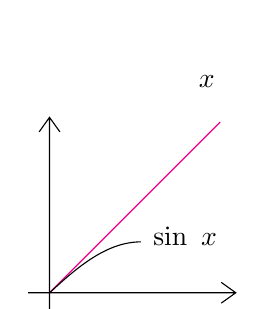
\begin{tikzpicture}[x=0.75pt,y=0.75pt,yscale=-1,xscale=1]
    %uncomment if require: \path (0,300); %set diagram left start at 0, and has height of 300
    
    %Shape: Axis 2D [id:dp008141030370613311] 
    \draw  (50,162.51) -- (150,162.51)(60.26,78) -- (60.26,178) (143,157.51) -- (150,162.51) -- (143,167.51) (55.26,85) -- (60.26,78) -- (65.26,85)  ;
    %Straight Lines [id:da3006663806705201] 
    \draw [color=magenta  ,draw opacity=1 ]   (60.26,162.51) -- (142.51,80.26) ;
    %Shape: Wave [id:dp8304296493911976] 
    \draw   (104.26,138) .. controls (88.39,138) and (74.44,149.34) .. (60.26,162.59) ;
    
    % Text Node
    \draw (131,56.4) node [anchor=north west][inner sep=0.75pt]    {$x$};
    % Text Node
    \draw (109,129.4) node [anchor=north west][inner sep=0.75pt]    {$\sin \ x$};
    
    
    \end{tikzpicture}
    }
\begin{proof}
    Since $|\cos t|\leq 1$, \begin{align*}
        x-\sin x &= (x-\sin x)-(0-\sin 0)\\
        &= \int_{0}^{x}\underset{\geq 0}{\underbrace{1-\cos t}}\d t \qquad \text{by FTC}\\
        &\geq 0
    \end{align*}
\end{proof}

\proposition
In addition, $\cos x\geq 1-\frac{x^2}{2}$ for $x\geq 0$.\sidenote{These are the first 2 terms in the power series

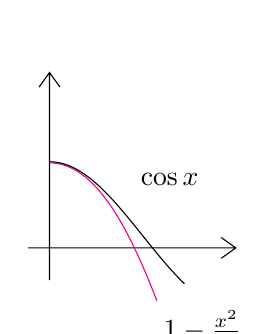
\begin{tikzpicture}[x=0.75pt,y=0.75pt,yscale=-1,xscale=1]
    %uncomment if require: \path (0,300); %set diagram left start at 0, and has height of 300
    
    %Shape: Axis 2D [id:dp008141030370613311] 
    \draw  (50,162.51) -- (150,162.51)(60.26,78) -- (60.26,178) (143,157.51) -- (150,162.51) -- (143,167.51) (55.26,85) -- (60.26,78) -- (65.26,85)  ;
    %Curve Lines [id:da027619260095050446] 
    \draw [color=magenta  ,draw opacity=1 ]   (60.13,121.51) .. controls (82.26,121.51) and (98.26,152.51) .. (112,188) ;
    %Shape: Wave [id:dp87403708438032] 
    \draw   (60.26,121) .. controls (76.54,121) and (90.58,138.44) .. (105.26,156.76) .. controls (111.96,165.13) and (118.54,173.32) .. (125.26,179.74) ;
    
    % Text Node
    \draw (114,191.4) node [anchor=north west][inner sep=0.75pt]    {$1-\frac{x^{2}}{2}$};
    % Text Node
    \draw (103,125.4) node [anchor=north west][inner sep=0.75pt]    {$\cos x$};
    
    
    \end{tikzpicture}
    }
\begin{proof}
    The previous prop gives:
    \begin{align*}
        \cos x -1 &= \cos x -\cos 0\\
        &= \int_{0}^{x}-\sin t\d t\\
        &\geq \int_{0}^{x}- t\d t\\
        &= \frac{-x^2}{2}
    \end{align*}
\end{proof}

\proposition Furthermore, for $x\geq 0$: \begin{itemize}
    \item $\sin x\geq x^3-\frac{x^3}{6}$
    \item $\cos x\leq 1-\frac{x^2}{2}+\frac{x^4}{24}$
\end{itemize}

\begin{proposition}
    There exists $x_0\in (0,\sqrt{3})$ such that $\cos x_0=0$.
   \[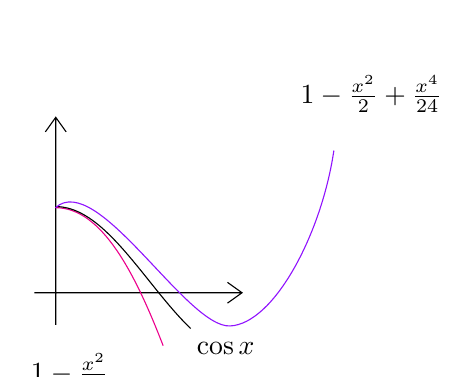
\begin{tikzpicture}[x=0.75pt,y=0.75pt,yscale=-1,xscale=1]
    %uncomment if require: \path (0,300); %set diagram left start at 0, and has height of 300
    
    %Shape: Axis 2D [id:dp008141030370613311] 
    \draw  (50,162.51) -- (150,162.51)(60.26,78) -- (60.26,178) (143,157.51) -- (150,162.51) -- (143,167.51) (55.26,85) -- (60.26,78) -- (65.26,85)  ;
    %Curve Lines [id:da027619260095050446] 
    \draw [color=magenta  ,draw opacity=1 ]   (60.13,121.51) .. controls (82.26,121.51) and (98.26,152.51) .. (112,188) ;
    %Shape: Wave [id:dp87403708438032] 
    \draw   (60.26,121) .. controls (76.54,121) and (90.58,138.44) .. (105.26,156.76) .. controls (111.96,165.13) and (118.54,173.32) .. (125.26,179.74) ;
    %Curve Lines [id:da00092922647570437] 
    \draw [color={rgb, 255:red, 144; green, 19; blue, 254 }  ,draw opacity=1 ]   (60.13,121.51) .. controls (80.26,103.51) and (123.26,179.51) .. (144.26,178.51) .. controls (165.26,177.51) and (188.26,134.51) .. (194.26,94) ;
    
    % Text Node
    \draw (47,190.4) node [anchor=north west][inner sep=0.75pt]    {$1-\frac{x^{2}}{2}$};
    % Text Node
    \draw (127,185.4) node [anchor=north west][inner sep=0.75pt]    {$\cos x$};
    % Text Node
    \draw (177,56.4) node [anchor=north west][inner sep=0.75pt]    {$1-\frac{x^{2}}{2} +\frac{x^{4}}{24}$};
    
    
    \end{tikzpicture}
    \]
\end{proposition}
\begin{proof}
    By the previous prop, we have $\cos \sqrt{3}\leq  1-\frac{\sqrt 3^2}{2}+\frac{\sqrt 3^4}{24}=\frac{1}{8}< 0$. Moreover, $\cos 0=1>0$, by IVT, there exists $x_0\in (0,\sqrt{3})$ such that $\cos x_0=0$.
\end{proof}

\begin{proposition}
    $\omega_0=4x_0$ is a period of $e^{iz}$. 
\end{proposition}
\begin{proof}
    Since $\cos x_0=0$, we have $\sin x_0=\pm 1$. Then $e^{ix_0}=\pm i$. We have $(\pm i)^4=1$, so $e^{4ix_0}=1=e^{0}$, so $\omega_0=4x_0$ is a period of $e^{iz}$.
\end{proof}

\begin{proposition}
    $\omega_0$ is the \textit{smallest} positive period of $e^{iz}$.
\end{proposition}

\begin{proposition}
    All periods of $e^{iz}$ are integer multiples of $2\pi=4x_0$.
\end{proposition}

\begin{proof}
    Define $\pi=2x_0$. The area of unit circle is \begin{align*}
        4\int_{0}^{1}\sqrt{1-x^2}\d x &= 4\int_{0}^{\frac{\pi}{2}}\sqrt{1-\sin^2 \theta}\d \theta\\
        &= 4\int_{0}^{\frac{\pi}{2}}\frac{1}{2}(1+\cos 2\theta)\d \theta\\
        &= \pi
    \end{align*}
\end{proof}

\subsection{Complex logarithm}
We know: $e^0=1,e^1=\sum_{n=0}^{\infty}\frac{1}{n!}=2.718\dots$

Since $\frac{\d}{\d x}e^x=e^x$, it is positive. If $x>0$, we conclude that $e^x$ is strictly increasing! As $e^x=\sum_{n=0}^{\infty}\frac{x^n}{n!}>1+x$, so $\lim_{x\to \infty}e^x=\infty$,

Therefore, $e^x$ is a \textbf{bijection} from $\R$ to $(0,\infty)$. This means it has an inverse that is a bijection from $(0,\infty)$ to $\R$.

\defn $\ln x$ is the inverse of $e^x$ for $x\in (0,+\infty)$.

Now what about the complex case? Let $z\neq 0$ and $z=re^{i\theta}$\sidenote{cf. trig properties} where $r=|z|>0$ and $\theta=\arg z\in \R$.\sidenote{Only determined up to addition of multiples of $2\pi$}

Hence, $z=re^{i\theta}=e^{\ln r}e^{i\theta}=e^{\ln r+i\theta}$. However, the $\theta$ is ambiguous to addition of multiples of $2\pi$!

\addlink{Logarithm}
\defn If $z\neq 0$, a \textbf{logarithm} of $z$ is a $w\in \C$ such that $e^{w}=z$.

We could graph the function $e^z$ with $z\in \C$:       
\[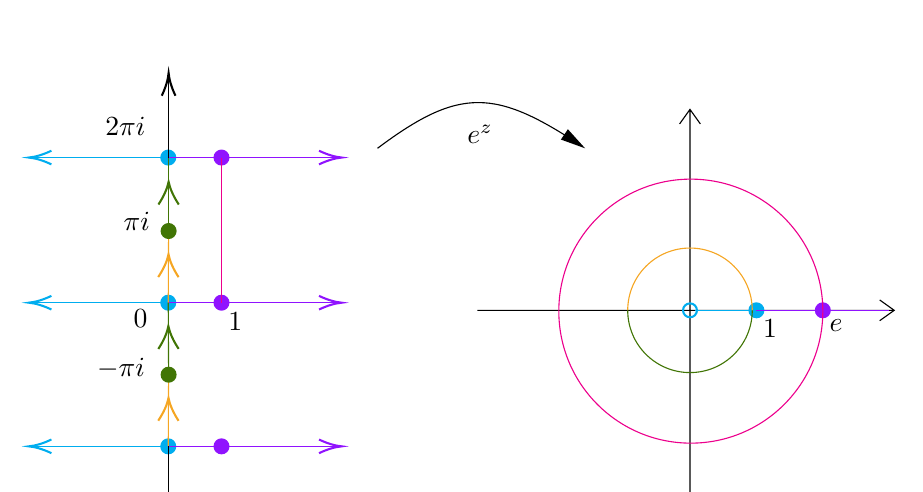
\begin{tikzpicture}[x=0.75pt,y=0.75pt,yscale=-1,xscale=1]
    %uncomment if require: \path (0,300); %set diagram left start at 0, and has height of 300
    
    %Straight Lines [id:da8785590871760756] 
    \draw [color={rgb, 255:red, 144; green, 19; blue, 254 }  ,draw opacity=1 ]   (145.63,130.39) -- (201.55,130.39) ;
    \draw [shift={(203.55,130.39)}, rotate = 180] [color={rgb, 255:red, 144; green, 19; blue, 254 }  ,draw opacity=1 ][line width=0.75]    (10.93,-3.29) .. controls (6.95,-1.4) and (3.31,-0.3) .. (0,0) .. controls (3.31,0.3) and (6.95,1.4) .. (10.93,3.29)   ;
    %Straight Lines [id:da1618236675525775] 
    \draw [color=cyan  ,draw opacity=1 ]   (119.98,130.39) -- (54.75,130.39) ;
    \draw [shift={(52.75,130.39)}, rotate = 360] [color=cyan  ,draw opacity=1 ][line width=0.75]    (10.93,-3.29) .. controls (6.95,-1.4) and (3.31,-0.3) .. (0,0) .. controls (3.31,0.3) and (6.95,1.4) .. (10.93,3.29)   ;
    \draw [shift={(119.98,130.39)}, rotate = 180] [color=cyan  ,draw opacity=1 ][fill=cyan  ,fill opacity=1 ][line width=0.75]      (0, 0) circle [x radius= 3.35, y radius= 3.35]   ;
    %Straight Lines [id:da8267712506988469] 
    \draw [color={rgb, 255:red, 144; green, 19; blue, 254 }  ,draw opacity=1 ]   (119.98,130.39) -- (145.63,130.39) ;
    \draw [shift={(145.63,130.39)}, rotate = 0] [color={rgb, 255:red, 144; green, 19; blue, 254 }  ,draw opacity=1 ][fill={rgb, 255:red, 144; green, 19; blue, 254 }  ,fill opacity=1 ][line width=0.75]      (0, 0) circle [x radius= 3.35, y radius= 3.35]   ;
    %Straight Lines [id:da2374921790479616] 
    \draw [color={rgb, 255:red, 144; green, 19; blue, 254 }  ,draw opacity=1 ]   (145.63,199.6) -- (201.55,199.6) ;
    \draw [shift={(203.55,199.6)}, rotate = 180] [color={rgb, 255:red, 144; green, 19; blue, 254 }  ,draw opacity=1 ][line width=0.75]    (10.93,-3.29) .. controls (6.95,-1.4) and (3.31,-0.3) .. (0,0) .. controls (3.31,0.3) and (6.95,1.4) .. (10.93,3.29)   ;
    %Straight Lines [id:da03468902350963088] 
    \draw [color=cyan  ,draw opacity=1 ]   (119.98,199.6) -- (54.75,199.6) ;
    \draw [shift={(52.75,199.6)}, rotate = 360] [color=cyan  ,draw opacity=1 ][line width=0.75]    (10.93,-3.29) .. controls (6.95,-1.4) and (3.31,-0.3) .. (0,0) .. controls (3.31,0.3) and (6.95,1.4) .. (10.93,3.29)   ;
    \draw [shift={(119.98,199.6)}, rotate = 180] [color=cyan  ,draw opacity=1 ][fill=cyan  ,fill opacity=1 ][line width=0.75]      (0, 0) circle [x radius= 3.35, y radius= 3.35]   ;
    %Straight Lines [id:da3208922622885413] 
    \draw [color={rgb, 255:red, 144; green, 19; blue, 254 }  ,draw opacity=1 ]   (119.98,199.6) -- (145.63,199.6) ;
    \draw [shift={(145.63,199.6)}, rotate = 0] [color={rgb, 255:red, 144; green, 19; blue, 254 }  ,draw opacity=1 ][fill={rgb, 255:red, 144; green, 19; blue, 254 }  ,fill opacity=1 ][line width=0.75]      (0, 0) circle [x radius= 3.35, y radius= 3.35]   ;
    %Straight Lines [id:da4709032693595072] 
    \draw [color={rgb, 255:red, 144; green, 19; blue, 254 }  ,draw opacity=1 ]   (145.63,60.46) -- (201.55,60.46) ;
    \draw [shift={(203.55,60.46)}, rotate = 180] [color={rgb, 255:red, 144; green, 19; blue, 254 }  ,draw opacity=1 ][line width=0.75]    (10.93,-3.29) .. controls (6.95,-1.4) and (3.31,-0.3) .. (0,0) .. controls (3.31,0.3) and (6.95,1.4) .. (10.93,3.29)   ;
    %Straight Lines [id:da05828217640270972] 
    \draw [color=cyan  ,draw opacity=1 ]   (119.98,60.46) -- (54.75,60.46) ;
    \draw [shift={(52.75,60.46)}, rotate = 360] [color=cyan  ,draw opacity=1 ][line width=0.75]    (10.93,-3.29) .. controls (6.95,-1.4) and (3.31,-0.3) .. (0,0) .. controls (3.31,0.3) and (6.95,1.4) .. (10.93,3.29)   ;
    \draw [shift={(119.98,60.46)}, rotate = 180] [color=cyan  ,draw opacity=1 ][fill=cyan  ,fill opacity=1 ][line width=0.75]      (0, 0) circle [x radius= 3.35, y radius= 3.35]   ;
    %Straight Lines [id:da6226539504724369] 
    \draw [color={rgb, 255:red, 144; green, 19; blue, 254 }  ,draw opacity=1 ]   (119.98,60.46) -- (145.63,60.46) ;
    \draw [shift={(145.63,60.46)}, rotate = 0] [color={rgb, 255:red, 144; green, 19; blue, 254 }  ,draw opacity=1 ][fill={rgb, 255:red, 144; green, 19; blue, 254 }  ,fill opacity=1 ][line width=0.75]      (0, 0) circle [x radius= 3.35, y radius= 3.35]   ;
    %Straight Lines [id:da35528692959663144] 
    \draw [color={rgb, 255:red, 245; green, 166; blue, 35 }  ,draw opacity=1 ]   (119.98,130.39) -- (120.15,95.86) ;
    \draw [shift={(120.1,107.13)}, rotate = 90.28] [color={rgb, 255:red, 245; green, 166; blue, 35 }  ,draw opacity=1 ][line width=0.75]    (10.93,-4.9) .. controls (6.95,-2.3) and (3.31,-0.67) .. (0,0) .. controls (3.31,0.67) and (6.95,2.3) .. (10.93,4.9)   ;
    %Straight Lines [id:da8648044267590989] 
    \draw [color={rgb, 255:red, 65; green, 117; blue, 5 }  ,draw opacity=1 ]   (120.15,95.86) -- (120.15,60.46) ;
    \draw [shift={(120.15,72.16)}, rotate = 90] [color={rgb, 255:red, 65; green, 117; blue, 5 }  ,draw opacity=1 ][line width=0.75]    (10.93,-4.9) .. controls (6.95,-2.3) and (3.31,-0.67) .. (0,0) .. controls (3.31,0.67) and (6.95,2.3) .. (10.93,4.9)   ;
    \draw [shift={(120.15,95.86)}, rotate = 270] [color={rgb, 255:red, 65; green, 117; blue, 5 }  ,draw opacity=1 ][fill={rgb, 255:red, 65; green, 117; blue, 5 }  ,fill opacity=1 ][line width=0.75]      (0, 0) circle [x radius= 3.35, y radius= 3.35]   ;
    %Straight Lines [id:da878911184832804] 
    \draw [color={rgb, 255:red, 245; green, 166; blue, 35 }  ,draw opacity=1 ]   (119.98,199.6) -- (120.15,165.07) ;
    \draw [shift={(120.1,176.34)}, rotate = 90.28] [color={rgb, 255:red, 245; green, 166; blue, 35 }  ,draw opacity=1 ][line width=0.75]    (10.93,-4.9) .. controls (6.95,-2.3) and (3.31,-0.67) .. (0,0) .. controls (3.31,0.67) and (6.95,2.3) .. (10.93,4.9)   ;
    %Straight Lines [id:da0013946467543932695] 
    \draw [color={rgb, 255:red, 65; green, 117; blue, 5 }  ,draw opacity=1 ]   (120.15,165.07) -- (119.98,130.39) ;
    \draw [shift={(120.04,141.73)}, rotate = 89.72] [color={rgb, 255:red, 65; green, 117; blue, 5 }  ,draw opacity=1 ][line width=0.75]    (10.93,-4.9) .. controls (6.95,-2.3) and (3.31,-0.67) .. (0,0) .. controls (3.31,0.67) and (6.95,2.3) .. (10.93,4.9)   ;
    \draw [shift={(120.15,165.07)}, rotate = 269.72] [color={rgb, 255:red, 65; green, 117; blue, 5 }  ,draw opacity=1 ][fill={rgb, 255:red, 65; green, 117; blue, 5 }  ,fill opacity=1 ][line width=0.75]      (0, 0) circle [x radius= 3.35, y radius= 3.35]   ;
    %Straight Lines [id:da6431192925230409] 
    \draw    (120.15,60.46) -- (120.15,21.72) ;
    \draw [shift={(120.15,19.72)}, rotate = 90] [color=black  ][line width=0.75]    (10.93,-3.29) .. controls (6.95,-1.4) and (3.31,-0.3) .. (0,0) .. controls (3.31,0.3) and (6.95,1.4) .. (10.93,3.29)   ;
    %Straight Lines [id:da4817110891560017] 
    \draw    (119.98,225.34) -- (119.98,199.6) ;
    %Curve Lines [id:da15130320225307914] 
    \draw    (220.8,56) .. controls (260.4,26.3) and (277.71,27.23) .. (319.53,55.15) ;
    \draw [shift={(320.8,56)}, rotate = 213.92] [fill=black  ][line width=0.08]  [draw opacity=0] (12,-3) -- (0,0) -- (12,3) -- cycle    ;
    %Shape: Axis 2D [id:dp10703039654547442] 
    \draw  (268.95,134.06) -- (469.75,134.06)(371.35,37.26) -- (371.35,229.26) (462.75,129.06) -- (469.75,134.06) -- (462.75,139.06) (366.35,44.26) -- (371.35,37.26) -- (376.35,44.26)  ;
    %Straight Lines [id:da39023709471268675] 
    \draw [color=cyan  ,draw opacity=1 ]   (373.7,134.06) -- (403.35,134.06) ;
    \draw [shift={(403.35,134.06)}, rotate = 0] [color=cyan  ,draw opacity=1 ][fill=cyan  ,fill opacity=1 ][line width=0.75]      (0, 0) circle [x radius= 3.35, y radius= 3.35]   ;
    \draw [shift={(371.35,134.06)}, rotate = 0] [color=cyan  ,draw opacity=1 ][line width=0.75]      (0, 0) circle [x radius= 3.35, y radius= 3.35]   ;
    %Straight Lines [id:da20992201553768708] 
    \draw [color={rgb, 255:red, 144; green, 19; blue, 254 }  ,draw opacity=1 ]   (435.35,134.06) -- (467.35,134.06) ;
    \draw [shift={(435.35,134.06)}, rotate = 0] [color={rgb, 255:red, 144; green, 19; blue, 254 }  ,draw opacity=1 ][fill={rgb, 255:red, 144; green, 19; blue, 254 }  ,fill opacity=1 ][line width=0.75]      (0, 0) circle [x radius= 3.35, y radius= 3.35]   ;
    %Straight Lines [id:da895300882766211] 
    \draw [color={rgb, 255:red, 144; green, 19; blue, 254 }  ,draw opacity=1 ]   (403.35,134.06) -- (435.35,134.06) ;
    %Shape: Arc [id:dp17152249012602994] 
    \draw  [draw opacity=0] (341.35,134.06) .. controls (341.35,134.06) and (341.35,134.06) .. (341.35,134.06) .. controls (341.35,117.49) and (354.78,104.06) .. (371.35,104.06) .. controls (387.92,104.06) and (401.35,117.49) .. (401.35,134.06) .. controls (401.35,134.06) and (401.35,134.06) .. (401.35,134.06) -- (371.35,134.06) -- cycle ; \draw [color={rgb, 255:red, 245; green, 166; blue, 35 }  ,draw opacity=1 ]   (341.35,134.06) .. controls (341.35,117.49) and (354.78,104.06) .. (371.35,104.06) .. controls (387.92,104.06) and (401.35,117.49) .. (401.35,134.06) ;  
    %Shape: Arc [id:dp054572774151422365] 
    \draw  [draw opacity=0] (401.35,134.06) .. controls (401.35,134.06) and (401.35,134.06) .. (401.35,134.06) .. controls (401.35,150.63) and (387.92,164.06) .. (371.35,164.06) .. controls (354.78,164.06) and (341.35,150.63) .. (341.35,134.06) .. controls (341.35,134.06) and (341.35,134.06) .. (341.35,134.06) -- (371.35,134.06) -- cycle ; \draw [color={rgb, 255:red, 65; green, 117; blue, 5 }  ,draw opacity=1 ]   (401.35,134.06) .. controls (401.35,150.63) and (387.92,164.06) .. (371.35,164.06) .. controls (354.78,164.06) and (341.35,150.63) .. (341.35,134.06) ;  
    %Straight Lines [id:da7090062681421083] 
    \draw [color=magenta  ,draw opacity=1 ]   (145.63,60.46) -- (145.63,130.39) ;
    %Shape: Circle [id:dp2705523730959791] 
    \draw  [color=magenta  ,draw opacity=1 ] (308.15,134.46) .. controls (308.15,99.34) and (336.63,70.86) .. (371.75,70.86) .. controls (406.88,70.86) and (435.35,99.34) .. (435.35,134.46) .. controls (435.35,169.59) and (406.88,198.06) .. (371.75,198.06) .. controls (336.63,198.06) and (308.15,169.59) .. (308.15,134.46) -- cycle ;
    
    % Text Node
    \draw (102,132.4) node [anchor=north west][inner sep=0.75pt]    {$0$};
    % Text Node
    \draw (147.63,133.79) node [anchor=north west][inner sep=0.75pt]    {$1$};
    % Text Node
    \draw (88.4,40) node [anchor=north west][inner sep=0.75pt]    {$2\pi i$};
    % Text Node
    \draw (97.2,85.6) node [anchor=north west][inner sep=0.75pt]    {$\pi i$};
    % Text Node
    \draw (84.4,156) node [anchor=north west][inner sep=0.75pt]    {$-\pi i$};
    % Text Node
    \draw (262.8,43.4) node [anchor=north west][inner sep=0.75pt]    {$e^{z}$};
    % Text Node
    \draw (405.35,137.46) node [anchor=north west][inner sep=0.75pt]    {$1$};
    % Text Node
    \draw (437.35,137.46) node [anchor=north west][inner sep=0.75pt]    {$e$};
    
    
    \end{tikzpicture}
    \]

\defn If $\Omega$ is a region in $\C$, then a continuous $l:\Omega \to \C$ is a \textbf{branch} of the logarithm if $e^{l(z)}=z$ for all $z\in \Omega$.\sidenote{note $0\notin \Omega$}

\addlink{Principal branch of the logarithm}
\eg If $\Omega=\C\backslash(-\infty, 0]$ such that $\theta\in (-\pi,\pi)$, a logarithm could be defined on it. This is the \textbf{principal branch} of the logarithm.\sidenote{See \href{https://stephangarcia.sites.pomona.edu/teaching/24S-135/Lecture/24S-135-Lecture10.pdf}{graphed Riemann surface}}

\addlink{First derivative of ln}
\rmk Suppose $l(z)$ is a branch of the logarithm and $l$ is analytic, then: \[e^{l(z)}=z\implies \frac{\d}{\d z}e^{l(z)} = l'(z)e^{l(z)}=1\]

Since $e^{l(z)}=z$, we conclude $l'(z)=\frac{1}{z}$.

\subsection{Complex power}
\defn If $z\neq 0$, \textit{define} $z^{a}=e^{a\log z}$.\sidenote{NOT well-defined!}

\rmk The definition of complex powers should coincide with the old one: $z^n=\underset{n}{\underbrace{z\cdot z\cdot\dots\cdot z}=r^ne^{in\theta}}$.

Check: \begin{align*}
    z^n&=e^{n\log z}=e^{n(\ln r+i\theta+i2\pi k)}\\
    &= e^{n\ln r}e^{in\theta}\underset{=1}{\underbrace{e^{i2\pi nk}}}\\
    &= r^ne^{in\theta}
\end{align*} is true for any $k\in \Z$.

How about $n$-th roots?
\begin{align*}
    z^{\frac{1}{n}} &= e^{\frac{1}{n}\log z}\\
    &= e^{\frac{1}{n}(\ln r+i\theta+i2\pi k)}\\
    &= e^{\frac{1}{n}\ln r}e^{\frac{i\theta}{n}}\underset{\text{$n$ distinct}}{\underbrace{e^{\frac{i2\pi k}{n}}}}\\
    &= r^{\frac{1}{n}} e^{i\left(\frac{\theta+2\pi k}{n}\right)}
\end{align*}

\subsection{Riemann surface}
We still have a problem: $\ln z$ is still not a function on $\C$! The branch depends on the arbitrary choice of domain. What shall we do to make it not dependent on a choice?

Answer: let $\ln$ not live on the complex plane, but  infinitely many copies of the slit plane $\C\backslash(-\infty, 0]$, each
one being glued to the next along the slit $(-\infty, 0]$.

\eg $z^{1/2}$ would live on a surface:
\[\begin{tikzpicture}[x=0.75pt,y=0.75pt,yscale=-1,xscale=1]
    %uncomment if require: \path (0,300); %set diagram left start at 0, and has height of 300
    
    %Straight Lines [id:da9680702032506614] 
    \draw [color=magenta  ,draw opacity=1 ] [dash pattern={on 4.5pt off 4.5pt}]  (124.85,130) -- (33.35,130) ;
    \draw [shift={(31.35,130)}, rotate = 360] [color=magenta  ,draw opacity=1 ][line width=0.75]    (10.93,-3.29) .. controls (6.95,-1.4) and (3.31,-0.3) .. (0,0) .. controls (3.31,0.3) and (6.95,1.4) .. (10.93,3.29)   ;
    \draw [shift={(127.2,130)}, rotate = 180] [color=magenta  ,draw opacity=1 ][line width=0.75]      (0, 0) circle [x radius= 3.35, y radius= 3.35]   ;
    %Shape: Arc [id:dp6906978961263923] 
    \draw  [draw opacity=0] (86.68,130) .. controls (86.68,130) and (86.68,130) .. (86.68,130) .. controls (86.68,107.62) and (104.82,89.48) .. (127.2,89.48) .. controls (149.58,89.48) and (167.72,107.62) .. (167.72,130) -- (127.2,130) -- cycle ; \draw [color={rgb, 255:red, 245; green, 166; blue, 35 }  ,draw opacity=1 ]   (86.68,130) .. controls (86.68,130) and (86.68,130) .. (86.68,130) .. controls (86.68,107.62) and (104.82,89.48) .. (127.2,89.48) .. controls (149.58,89.48) and (167.72,107.62) .. (167.72,130) ;  
    %Shape: Arc [id:dp9861691627816211] 
    \draw  [draw opacity=0] (167.72,130) .. controls (167.72,130) and (167.72,130) .. (167.72,130) .. controls (167.72,152.38) and (149.58,170.52) .. (127.2,170.52) .. controls (104.82,170.52) and (86.68,152.38) .. (86.68,130) -- (127.2,130) -- cycle ; \draw [color={rgb, 255:red, 65; green, 117; blue, 5 }  ,draw opacity=1 ]   (167.72,130) .. controls (167.72,130) and (167.72,130) .. (167.72,130) .. controls (167.72,152.38) and (149.58,170.52) .. (127.2,170.52) .. controls (104.82,170.52) and (86.68,152.38) .. (86.68,130) ;  
    %Straight Lines [id:da9124411332810323] 
    \draw [color=magenta  ,draw opacity=1 ] [dash pattern={on 4.5pt off 4.5pt}]  (318.45,130) -- (226.95,130) ;
    \draw [shift={(224.95,130)}, rotate = 360] [color=magenta  ,draw opacity=1 ][line width=0.75]    (10.93,-3.29) .. controls (6.95,-1.4) and (3.31,-0.3) .. (0,0) .. controls (3.31,0.3) and (6.95,1.4) .. (10.93,3.29)   ;
    \draw [shift={(320.8,130)}, rotate = 180] [color=magenta  ,draw opacity=1 ][line width=0.75]      (0, 0) circle [x radius= 3.35, y radius= 3.35]   ;
    %Shape: Arc [id:dp05520981510099365] 
    \draw  [draw opacity=0] (280.28,130) .. controls (280.28,107.62) and (298.42,89.48) .. (320.8,89.48) .. controls (343.18,89.48) and (361.32,107.62) .. (361.32,130) -- (320.8,130) -- cycle ; \draw [color={rgb, 255:red, 65; green, 117; blue, 5 }  ,draw opacity=1 ]   (280.28,130) .. controls (280.28,107.62) and (298.42,89.48) .. (320.8,89.48) .. controls (343.18,89.48) and (361.32,107.62) .. (361.32,130) ;  
    %Shape: Arc [id:dp5073887586255386] 
    \draw  [draw opacity=0] (361.32,130) .. controls (361.32,130) and (361.32,130) .. (361.32,130) .. controls (361.32,130) and (361.32,130) .. (361.32,130) .. controls (361.32,152.38) and (343.18,170.52) .. (320.8,170.52) .. controls (298.42,170.52) and (280.28,152.38) .. (280.28,130) -- (320.8,130) -- cycle ; \draw [color={rgb, 255:red, 245; green, 166; blue, 35 }  ,draw opacity=1 ]   (361.32,130) .. controls (361.32,130) and (361.32,130) .. (361.32,130) .. controls (361.32,152.38) and (343.18,170.52) .. (320.8,170.52) .. controls (298.42,170.52) and (280.28,152.38) .. (280.28,130) ;  
    
    % Text Node
    \draw (171.6,124.6) node [anchor=north west][inner sep=0.75pt]    {$1$};
    % Text Node
    \draw (70.8,109.2) node [anchor=north west][inner sep=0.75pt]    {$i$};
    % Text Node
    \draw (367.6,122.8) node [anchor=north west][inner sep=0.75pt]    {$-1$};
    % Text Node
    \draw (258.8,106.8) node [anchor=north west][inner sep=0.75pt]    {$-i$};
    
    
    \end{tikzpicture}
    \]

\section{Cauchy's theorem and its consequences}

\subsection{Complex integration}
\addlink{Piecewise continuity}
\defn A complex-valued function $\gamma:[a,b]\to \C$ is \textbf{piecewise} continuous if $\gamma$ is continuous at all but \textit{finitely many} points of $[a,b]$ and $\gamma$ has one-sided limits that are \textit{finite} at each point (of discontinuity).

\[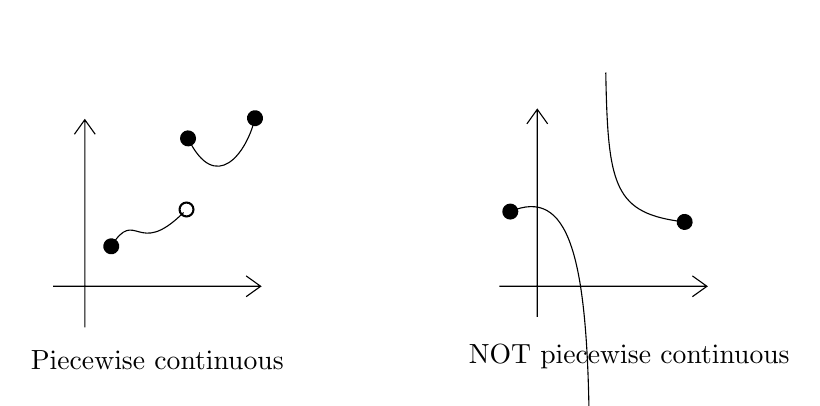
\begin{tikzpicture}[x=0.75pt,y=0.75pt,yscale=-1,xscale=1]
    %uncomment if require: \path (0,300); %set diagram left start at 0, and has height of 300
    
    %Shape: Axis 2D [id:dp7003951674563056] 
    \draw  (50,158.26) -- (150,158.26)(65.26,78) -- (65.26,178) (143,153.26) -- (150,158.26) -- (143,163.26) (60.26,85) -- (65.26,78) -- (70.26,85)  ;
    %Curve Lines [id:da5314714499980906] 
    \draw    (78,139) .. controls (90.01,119.66) and (90.25,145.2) .. (112.84,122.7) ;
    \draw [shift={(114.26,121.26)}, rotate = 313.83] [color=black  ][line width=0.75]      (0, 0) circle [x radius= 3.35, y radius= 3.35]   ;
    \draw [shift={(78,139)}, rotate = 301.84] [color=black  ][fill=black  ][line width=0.75]      (0, 0) circle [x radius= 3.35, y radius= 3.35]   ;
    %Curve Lines [id:da27910409809362413] 
    \draw    (115,87) .. controls (128.26,114.26) and (143.26,94.26) .. (147.26,77.26) ;
    \draw [shift={(147.26,77.26)}, rotate = 283.24] [color=black  ][fill=black  ][line width=0.75]      (0, 0) circle [x radius= 3.35, y radius= 3.35]   ;
    \draw [shift={(115,87)}, rotate = 64.07] [color=black  ][fill=black  ][line width=0.75]      (0, 0) circle [x radius= 3.35, y radius= 3.35]   ;
    %Shape: Axis 2D [id:dp8923800564332263] 
    \draw  (265,158.26) -- (365,158.26)(283.26,73) -- (283.26,173) (358,153.26) -- (365,158.26) -- (358,163.26) (278.26,80) -- (283.26,73) -- (288.26,80)  ;
    %Curve Lines [id:da7330323189044972] 
    \draw    (270.26,122.26) .. controls (298.26,110.26) and (307.26,143.26) .. (308.26,223.26) ;
    \draw [shift={(270.26,122.26)}, rotate = 336.8] [color=black  ][fill=black  ][line width=0.75]      (0, 0) circle [x radius= 3.35, y radius= 3.35]   ;
    %Curve Lines [id:da7451055597374061] 
    \draw    (354.26,127.26) .. controls (320.26,123.26) and (317.26,110.26) .. (316.26,55.26) ;
    \draw [shift={(354.26,127.26)}, rotate = 186.71] [color=black  ][fill=black  ][line width=0.75]      (0, 0) circle [x radius= 3.35, y radius= 3.35]   ;
    
    % Text Node
    \draw (38,188) node [anchor=north west][inner sep=0.75pt]   [align=left] {Piecewise continuous};
    % Text Node
    \draw (249,185) node [anchor=north west][inner sep=0.75pt]   [align=left] {NOT piecewise continuous};
    
    
    \end{tikzpicture}\]

If $\gamma$ is piecewise continuous, then $\int_{a}^{b}\re \gamma(t)\d t$ and $\int_{a}^{b}\im \gamma(t)\d t$ exist. Then we define \textbf{complex integration}:
\[\int_{a}^{b}\gamma(t)\d t = \int_{a}^{b}\re \gamma(t)\d t +i\cdot \int_{a}^{b}\im \gamma(t)\d t\]

That is, \begin{align*}
    \re \left(\int_{a}^{b}\gamma(t)\d t\right)&=\int_{a}^{b}\re \gamma(t)\d t\\
    \im \left(\int_{a}^{b}\gamma(t)\d t\right)&=\int_{a}^{b}\im \gamma(t)\d t\\
\end{align*}

In addition, if $\gamma_1,\gamma_2$ are both $[a,b]\to \C$ and piecewise cont., and $c_1,c_2\in\C$, then \[\int_{a}^{b}\left( c_1\gamma_1(t)+c_2\gamma_2(t) \right)\d t=c_1\int_{a}^{b}\gamma_1(t)\d t+c_2\int_{a}^{b}\gamma_2(t)\d t\]

\addlink{Triangle inequality}
\begin{proposition}[Triangle inequality]
    If $\gamma:[a,b]\to \C$ is {piecewise} continuous, then \[\left|\int_{a}^{b}\gamma(t)\d t \right|\leq \int_{a}^{b}|\gamma(t)|\d t \]
\end{proposition}
\begin{proof}
    WLOG assume $ \int_{a}^{b}\gamma(t)\d t \neq 0$. Define $\lambda = \frac{\left|\int_{a}^{b}\gamma(t)\d t\right|}{\int_{a}^{b}\gamma(t)\d t}$ and note $|\lambda|=1$.

    Thus, \begin{align*}
        \left|\int_{a}^{b}\gamma(t)\d t\right| &= \lambda\int_{a}^{b}\gamma(t)\d t\\
        &= \int_{a}^{b}\lambda\gamma(t)\d t &&\text{because LHS is }\in \R\\
        &= \re \int_{a}^{b}\lambda\gamma(t)\d t\\
        &\leq \int_{a}^{b}|\lambda\gamma(t)|\d t &&\because \re z\leq |z|\\
        &= \int_{a}^{b}|\gamma(t)|\d t&& \because |\lambda|=1
    \end{align*}
\end{proof}

\subsubsection{Complex differentiability}
\defn $\gamma:[a,b]\to \C$ is \textbf{differentiable} at $t\in [a,b]$ if $\re \gamma$ and $\im \gamma$ are differentiable (in the sense of real variables). We define \[\gamma'(t)=(\re \gamma)'(t)+i\cdot (\im \gamma)'(t)\]

\defn $\gamma:[a,b]\to \C$ is \textbf{piecewise} $C^1$\sidenote{$C^1$ is one-time differentiable} if: \begin{enumerate}[label=(\alph*)]
    \item $\gamma$ is continuous on $[a,b]$.
    \item $\gamma$ is differentiable at all but finitely many points of $[a,b]$.
    \item $\gamma'$ is continuous at each point where it exists.
    \item $\gamma'$ has finite one-sided limits at every point of discontinuity.
\end{enumerate}

\subsubsection{Fundamental theorem of calculus, complex edition}
If $\gamma:[a,b]\to\C$ is piecewise $C^1$, then:
\[\int_{a}^{b}\gamma'(t)\d t=\gamma(b)-\gamma(a)\]

\defn If $\gamma$ is $C^1$, then the arclength
\sidenote{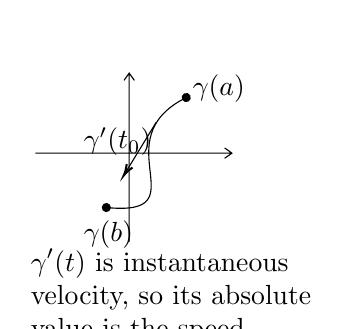
\begin{tikzpicture}[x=0.75pt,y=0.75pt,yscale=-0.5,xscale=0.5]
    %uncomment if require: \path (0,286); %set diagram left start at 0, and has height of 286
    
    %Shape: Axis 2D [id:dp5992461788507699] 
    \draw  (50,141.08) -- (239.26,141.08)(140.26,64) -- (140.26,226.51) (232.26,136.08) -- (239.26,141.08) -- (232.26,146.08) (135.26,71) -- (140.26,64) -- (145.26,71)  ;
    %Curve Lines [id:da8169369769076535] 
    \draw    (118.26,193.51) .. controls (210.26,202.51) and (113.26,128.51) .. (195.26,87.51) ;
    \draw [shift={(195.26,87.51)}, rotate = 333.43] [color=black  ][fill=black  ][line width=0.75]      (0, 0) circle [x radius= 3.35, y radius= 3.35]   ;
    \draw [shift={(118.26,193.51)}, rotate = 5.59] [color=black  ][fill=black  ][line width=0.75]      (0, 0) circle [x radius= 3.35, y radius= 3.35]   ;
    %Straight Lines [id:da7279313778056917] 
    \draw    (166.26,111.51) -- (136.05,160.92) ;
    \draw [shift={(135,162.63)}, rotate = 301.44] [color=black  ][line width=0.75]    (10.93,-3.29) .. controls (6.95,-1.4) and (3.31,-0.3) .. (0,0) .. controls (3.31,0.3) and (6.95,1.4) .. (10.93,3.29)   ;
    
    % Text Node
    \draw (199,63.4) node [anchor=north west][inner sep=0.75pt]    {$\gamma ( a)$};
    % Text Node
    \draw (94,203.4) node [anchor=north west][inner sep=0.75pt]    {$\gamma ( b)$};
    % Text Node
    \draw (94,114.4) node [anchor=north west][inner sep=0.75pt]    {$\gamma '( t_{0})$};
    % Text Node
    \draw (43,231) node [anchor=north west][inner sep=0.75pt]   [align=left] {$\displaystyle \gamma '( t)$ is instantaneous\\ velocity, so its absolute\\ value is the speed};
    
    
    \end{tikzpicture}
    } 
    of $\gamma$ is: \[L(\gamma)=\int_{a}^{b}|\gamma'(t)|\d t\]

\defn If $\gamma:[a,b]\to \reg$ is piecewise $C^1$ and $f:\reg \to\C$ is continuous, then \[\int_{\gamma}f(z)\d z=\int_{a}^{b}f(\gamma(t))\gamma'(t)\d t\]
where $z=\gamma(t)$ and $\d z=\gamma'(t)\d t$

We have \textbf{linearity} w.r.t. $f$: \[\int_{\gamma}\left( c_1f_1(z)+c_2f_2(z) \right)\d z=c_1\int_{\gamma}f_1(z)\d z+c_2\int_{\gamma}f_2(z)\d z\]

\rmk Arclength is independent from parameterization.
\begin{proof}
    Let $\gamma:[a,b]\to \reg$ be piecewise $C^1$. Let $\alpha:[c,d] \to [a,b]$ is an increasing, piecewise $C^1$ surjection such that $\alpha(c)=a, \alpha(d)=b$. Then $\phi=\gamma\circ \alpha:[c,d]\to \reg$ is also piecewise $C^1$. Hence, by substituting $s=\alpha(t), \d s=\alpha'(t)\d t$:
    \begin{align*}
        \int_{\phi}f(z)\d z&=\int_{c}^{d}f(\phi(t))\phi'(t)\d t\\
        &= \int_{c}^{d}f(\gamma(\alpha(t)))\gamma'(\alpha(t))\alpha'(t)\d t\\
        &= \int_{a}^{b}f(\gamma(s))\gamma'(s)\d s\\
        &= \int_{\gamma}f(z)\d z
    \end{align*}
\end{proof}

\subsubsection{An important estimate}
Let $f$ be continuous. Since \(\int_{\gamma}f(z)\d z=\int_{a}^{b}f(\gamma(t))\gamma'(t)\d t\), we observe: \begin{align*}
    \left|\int_{\gamma}f(z)\d z\right|&=\left|\int_{a}^{b}f(\gamma(t))\gamma'(t)\d t\right|\\
    &\leq \int_{a}^{b}|f(\gamma(t))|\,|\gamma'(t)|\d t\\
    &\leq \max_{t\in [a,b]}|f(\gamma(t))| \int_{a}^{b}|\gamma'(t)|\d t\\
    &= \rt{\max_{z\in \gamma}|f(z)|\cdot L(\gamma)}
\end{align*}


\defn If $\gamma:[a,b]\to\C$, the reverse of $\gamma$ is $(-\gamma):[-b,-a]\to\C$ defined by $(-\gamma)(t)=\gamma(-t)$. \sidenote{going around the track backwards} Hence, \[\int_{-\gamma}f(z)\d z= -\int_{\gamma}f(z)\d z\]

\rmk We can also break up the curve and integral the two parts separately: \sidenote{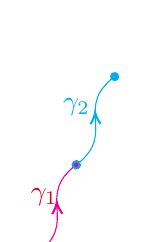
\begin{tikzpicture}[x=0.75pt,y=0.75pt,yscale=-0.5,xscale=0.5]
    %uncomment if require: \path (0,300); %set diagram left start at 0, and has height of 300
    
    %Curve Lines [id:da6510647213107017] 
    \draw [color=magenta  ,draw opacity=1 ]   (144.26,215.76) .. controls (184.26,185.76) and (141.26,160.76) .. (181.26,130.76) ;
    \draw [shift={(181.26,130.76)}, rotate = 323.13] [color=magenta  ,draw opacity=1 ][fill=magenta  ,fill opacity=1 ][line width=0.75]      (0, 0) circle [x radius= 3.35, y radius= 3.35]   ;
    \draw [shift={(162.49,167.07)}, rotate = 87.57] [color=magenta  ,draw opacity=1 ][line width=0.75]    (10.93,-4.9) .. controls (6.95,-2.3) and (3.31,-0.67) .. (0,0) .. controls (3.31,0.67) and (6.95,2.3) .. (10.93,4.9)   ;
    \draw [shift={(144.26,215.76)}, rotate = 323.13] [color=magenta  ,draw opacity=1 ][fill=magenta  ,fill opacity=1 ][line width=0.75]      (0, 0) circle [x radius= 3.35, y radius= 3.35]   ;
    %Curve Lines [id:da6697996530017996] 
    \draw [color=cyan  ,draw opacity=1 ]   (183.56,128.97) .. controls (219.57,99.76) and (179.06,75.16) .. (218.26,45.76) ;
    \draw [shift={(218.26,45.76)}, rotate = 323.13] [color=cyan  ,draw opacity=1 ][fill=cyan  ,fill opacity=1 ][line width=0.75]      (0, 0) circle [x radius= 3.35, y radius= 3.35]   ;
    \draw [shift={(199.47,80.56)}, rotate = 88.14] [color=cyan  ,draw opacity=1 ][line width=0.75]    (10.93,-4.9) .. controls (6.95,-2.3) and (3.31,-0.67) .. (0,0) .. controls (3.31,0.67) and (6.95,2.3) .. (10.93,4.9)   ;
    \draw [shift={(181.26,130.76)}, rotate = 323.13] [color=cyan  ,draw opacity=1 ][line width=0.75]      (0, 0) circle [x radius= 3.35, y radius= 3.35]   ;
    
    % Text Node
    \draw (135,151.4) node [anchor=north west][inner sep=0.75pt]    {$\textcolor[rgb]{0.82,0.01,0.11}{\gamma _{1}}$};
    % Text Node
    \draw (166,64.4) node [anchor=north west][inner sep=0.75pt]    {$\textcolor{cyan}{\gamma _{2}}$};
    
    
    \end{tikzpicture}
    }
\[\int_{\gamma}f(z)\d z = \int_{\gamma_1}f(z)\d z + \int_{\gamma_2}f(z)\d z\]

\subsubsection{Fundamental theorem of calculus for contour integrals}
If $\gamma:[a,b]\to\C$ is piecewise $C^1$, and $f:\reg\to \C$ is analytic \sidenote{Assuming $f'$ continuous, which we would prove later},
then \[\int_{\gamma}f'(z)\d z=f(\gamma(b))-f(\gamma(a))\]

If $\gamma(a)=\gamma(b)$, then $\int_{\gamma}f'(z)\d z=0$.

\begin{proof}
    \begin{align*}
        \int_{\gamma}f'(z)\d z&= \int_{a}^{b}f'(\gamma(t))\gamma'(t)\d t\\
        &= \int_{a}^{b}(f\circ \gamma)'(t)\d t &&\text{chain rule}\\
        &= f(\gamma(b))-f(\gamma(a))
    \end{align*}
\end{proof}

\eg Let $\gamma$ be a circle of radius $R$ centered at $z_0$: $\gamma(t)=z_0+Re^{it}\, ,t\in [0,2\pi]$. We would like to find \(\int_{\gamma}(z-z_0)^n\d z\).

If $n\neq -1$, then $\left(\frac{(z-z_0)^{n+1}}{n+1}\right)' = (z-z_0)^n$. Thus, \[\int_{\gamma}(z-z_0)^n\d z = \int_{\gamma}\left(\frac{(z-z_0)^{n+1}}{n+1}\right)'\d z =0\] by FTC. 

If $n=-1$, \[\int_{\gamma}(z-z_0)^n\d z= \int_{\gamma}\frac{1}{z-z_0}\d z = \int_{0}^{2\pi}i\d t=2\pi i\]

\subsection{Cauchy's theorem}
\subsubsection{Take 1}
\begin{theorem}[Cauchy's]\label[theorem]{cauchys-take1}
    Let $\reg$ be a region in $\C$ containing a \textit{simple}\sidenote{does not self-intersect} piecewise $C^1$ \textit{closed} curve $\gamma$ and its interior\sidenote{holes not allowed in the interior}.

    If $f:\reg \to \C$ is analytic, then $\int_{\gamma}f(z)\d z=0$.
    \[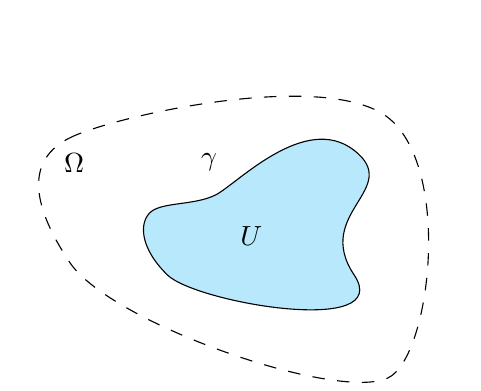
\begin{tikzpicture}[x=0.75pt,y=0.75pt,yscale=-1,xscale=1]
        %uncomment if require: \path (0,300); %set diagram left start at 0, and has height of 300
        
        %Shape: Polygon Curved [id:ds9387894112968782] 
        \draw  [fill=cyan  ,fill opacity=0.28 ] (163.26,91.51) .. controls (173.26,86.51) and (206.26,51.51) .. (230,70) .. controls (253.74,88.49) and (210,100) .. (230,130) .. controls (250,160) and (153.74,143.49) .. (140,130) .. controls (126.26,116.51) and (126.44,104.14) .. (132.26,99.51) .. controls (138.07,94.89) and (153.26,96.51) .. (163.26,91.51) -- cycle ;
        %Shape: Polygon Curved [id:ds6099513547861319] 
        \draw  [dash pattern={on 4.5pt off 4.5pt}] (93,64) .. controls (113,54) and (207.26,32.51) .. (242.26,51.51) .. controls (277.26,70.51) and (268.26,163.51) .. (248.26,178.51) .. controls (228.26,193.51) and (113,154) .. (93,124) .. controls (73,94) and (73,74) .. (93,64) -- cycle ;
        
        % Text Node
        \draw (89,70.4) node [anchor=north west][inner sep=0.75pt]    {${\Omega}$};
        % Text Node
        \draw (174,105.4) node [anchor=north west][inner sep=0.75pt]    {$U$};
        % Text Node
        \draw (155,70.4) node [anchor=north west][inner sep=0.75pt]    {$\gamma $};
        
        
        \end{tikzpicture}
        \]
\end{theorem}
\begin{proof}[``Proof'']
    Let $U$ be the union of $\gamma$ and its interior. Let $f=u+iv$ as usual, write $\d z = \d x + i\d y$:\begin{align*}
        \int_{\gamma}f(z)\d z &= \int_\gamma (u+iv)(\d x + i\d y)\\
        &= \int_\gamma u\d x-v\d y + i\int_{\gamma}v\d x +u\d y\\
        &= \int\int_{U}(-v_x-u_y)\d x\d y+i\int\int_{U}(u_x-v_y)\d x\d y &&\text{by Green's thm}\\
        &= 0 &&\text{by Cauchy-Riemann}
    \end{align*}
\end{proof}
However, this `proof' heavily relies on the fact that $u,v$ are $C^1$ and that the partial derivatives are continuous. This assumes $f'$ is continuous, but we aren't sure about that yet!\sidenote{See \hyperlink{goursats-lemma}{Goursat's Lemma}}

\subsubsection{Take 2: deformation version}
\begin{theorem}[Cauchy's]\label[theorem]{cauchys-take2-deform}
    Let $\gamma_1,\gamma_2$ be piecewise $C^1$ curves in a region $\Omega$ with the same start and end points. If $\gamma_1$ can be continuously deformed to $\gamma_2$ without ever passing outside of $\Omega$, then \[\int_{\gamma_1}f(z)\d z=\int_{\gamma_2}f(z)\d z\]
\end{theorem}
By the \textit{previous} statement of Cauchy's theorem (in \cref{cauchys-take1}), we observe that $\int_{\gamma_1-\gamma_2}f(z)\d z=0$, so this one falls out.

\noneg The $\gamma_1,\gamma_2$ in the picture below cannot be continuously deformed into each other!
\[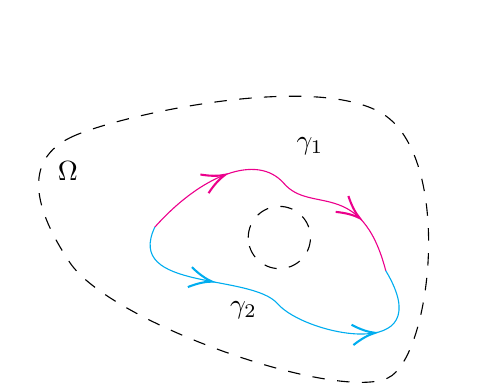
\begin{tikzpicture}[x=0.75pt,y=0.75pt,yscale=-1,xscale=1]
    %uncomment if require: \path (0,300); %set diagram left start at 0, and has height of 300
    
    %Shape: Polygon Curved [id:ds6460613846150254] 
    \draw  [dash pattern={on 4.5pt off 4.5pt}] (116,80) .. controls (136,70) and (230.26,48.51) .. (265.26,67.51) .. controls (300.26,86.51) and (291.26,179.51) .. (271.26,194.51) .. controls (251.26,209.51) and (136,170) .. (116,140) .. controls (96,110) and (96,90) .. (116,80) -- cycle ;
    %Curve Lines [id:da29780021147999514] 
    \draw [color=magenta  ,draw opacity=1 ]   (157,123) .. controls (179.26,98.01) and (206.26,87.01) .. (219.26,102.01) .. controls (232.26,117.01) and (256.51,99.03) .. (268.26,144.01) ;
    \draw [shift={(190.93,97.76)}, rotate = 156.33] [color=magenta  ,draw opacity=1 ][line width=0.75]    (10.93,-4.9) .. controls (6.95,-2.3) and (3.31,-0.67) .. (0,0) .. controls (3.31,0.67) and (6.95,2.3) .. (10.93,4.9)   ;
    \draw [shift={(255.72,118.67)}, rotate = 218.7] [color=magenta  ,draw opacity=1 ][line width=0.75]    (10.93,-4.9) .. controls (6.95,-2.3) and (3.31,-0.67) .. (0,0) .. controls (3.31,0.67) and (6.95,2.3) .. (10.93,4.9)   ;
    %Curve Lines [id:da7249434898522338] 
    \draw [color=cyan  ,draw opacity=1 ]   (157,123) .. controls (142.26,154.01) and (203.26,145.01) .. (216.26,160.01) .. controls (229.26,175.01) and (295.26,189.01) .. (268.26,144.01) ;
    \draw [shift={(184.59,149.25)}, rotate = 191.44] [color=cyan  ,draw opacity=1 ][line width=0.75]    (10.93,-4.9) .. controls (6.95,-2.3) and (3.31,-0.67) .. (0,0) .. controls (3.31,0.67) and (6.95,2.3) .. (10.93,4.9)   ;
    \draw [shift={(263.11,173.95)}, rotate = 174.82] [color=cyan  ,draw opacity=1 ][line width=0.75]    (10.93,-4.9) .. controls (6.95,-2.3) and (3.31,-0.67) .. (0,0) .. controls (3.31,0.67) and (6.95,2.3) .. (10.93,4.9)   ;
    %Shape: Circle [id:dp10939024496763072] 
    \draw  [dash pattern={on 4.5pt off 4.5pt}] (202,128.01) .. controls (202,119.73) and (208.71,113.01) .. (216.99,113.01) .. controls (225.27,113.01) and (231.99,119.73) .. (231.99,128.01) .. controls (231.99,136.29) and (225.27,143) .. (216.99,143) .. controls (208.71,143) and (202,136.29) .. (202,128.01) -- cycle ;
    
    % Text Node
    \draw (109,90.4) node [anchor=north west][inner sep=0.75pt]    {$\Omega $};
    % Text Node
    \draw (224,78.4) node [anchor=north west][inner sep=0.75pt]    {$\gamma _{1}$};
    % Text Node
    \draw (192,157.4) node [anchor=north west][inner sep=0.75pt]    {$\gamma _{2}$};
    
    
    \end{tikzpicture}
    \]

\subsection{Fresnel integrals}
Consider:
\[\int_{0}^{\infty}\sin (t^2)\d t \qquad \text{and} \qquad \int_{0}^{\infty}\cos (t^2)\d t\]
aka.
\[\lim_{R\to \infty}\int_{0}^{R}\sin (t^2)\d t \qquad \text{and} \qquad \lim_{R\to \infty}\int_{0}^{R}\cos (t^2)\d t\]
It's not obvious that these integrals converge!

Solution: PIZZA!
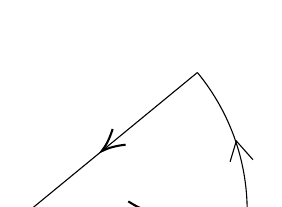
\begin{tikzpicture}[x=0.75pt,y=0.75pt,yscale=-1,xscale=1]
    %uncomment if require: \path (0,300); %set diagram left start at 0, and has height of 300
    
    %Straight Lines [id:da23065699869402656] 
    \draw    (100,126) -- (206.26,126) ;
    \draw [shift={(159.13,126)}, rotate = 180] [color=black  ][line width=0.75]    (10.93,-4.9) .. controls (6.95,-2.3) and (3.31,-0.67) .. (0,0) .. controls (3.31,0.67) and (6.95,2.3) .. (10.93,4.9)   ;
    %Shape: Arc [id:dp010225998094383515] 
    \draw  [draw opacity=0] (205.5,126.02) .. controls (205.5,126.01) and (205.5,126.01) .. (205.5,126) .. controls (205.5,100.56) and (196.5,77.23) .. (181.5,59.01) -- (100,126) -- cycle ; \draw   (205.5,126.02) .. controls (205.5,126.01) and (205.5,126.01) .. (205.5,126) .. controls (205.5,100.56) and (196.5,77.23) .. (181.5,59.01) ;  
    %Straight Lines [id:da5834097312816091] 
    \draw    (100,126) -- (181.5,59.01) ;
    \draw [shift={(135.34,96.95)}, rotate = 320.58] [color=black  ][line width=0.75]    (10.93,-4.9) .. controls (6.95,-2.3) and (3.31,-0.67) .. (0,0) .. controls (3.31,0.67) and (6.95,2.3) .. (10.93,4.9)   ;
    %Straight Lines [id:da6100230617755076] 
    \draw    (197.26,102.01) -- (200.26,92.01) -- (208.26,101.01) ;
    
    
    
    
    \end{tikzpicture}
Let $\gamma$ be the `sum' of all 3 curves as shown. Let $R\to \infty$. Then, by Cauchy's theorem, \(\int_\gamma e^{iz^2}\d z =0\).    

\ontangent{

\rmk We don't know how to write out the antiderivative of $f(z)=e^{iz^2}$ but we can use series!
\begin{align*}
    f(z) &= e^{iz^2}\\
    &= \sum_{n=0}^{\infty}\frac{(iz^2)^n}{n!}\\
    &= \sum_{n=0}^{\infty}\frac{i^nz^{2n}}{n!}
\end{align*}
And so \[F(z)=\sum_{n=0}^{\infty}\frac{i^nz^{2n+1}}{(2n+1)n!}\]

}

Now we return to the integral. Strategy: \[0= \int_\gamma e^{iz^2}\d  = \underset{I_1(R)}{\underbrace{\int_{\gamma_1} e^{iz^2}\d z}} + \underset{I_2(R)}{\underbrace{\int_{\gamma_2} e^{iz^2}\d z}} + \underset{I_3(R)}{\underbrace{\int_{\gamma_3} e^{iz^2}\d z}}\]

\[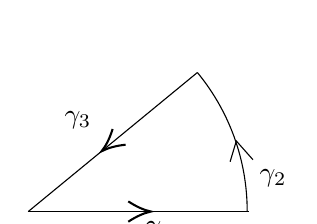
\begin{tikzpicture}[x=0.75pt,y=0.75pt,yscale=-1,xscale=1]
    %uncomment if require: \path (0,300); %set diagram left start at 0, and has height of 300
    
    %Straight Lines [id:da23065699869402656] 
    \draw    (100,126) -- (206.26,126) ;
    \draw [shift={(159.13,126)}, rotate = 180] [color=black  ][line width=0.75]    (10.93,-4.9) .. controls (6.95,-2.3) and (3.31,-0.67) .. (0,0) .. controls (3.31,0.67) and (6.95,2.3) .. (10.93,4.9)   ;
    %Shape: Arc [id:dp010225998094383515] 
    \draw  [draw opacity=0] (205.5,126.02) .. controls (205.5,126.01) and (205.5,126.01) .. (205.5,126) .. controls (205.5,100.56) and (196.5,77.23) .. (181.5,59.01) -- (100,126) -- cycle ; \draw   (205.5,126.02) .. controls (205.5,126.01) and (205.5,126.01) .. (205.5,126) .. controls (205.5,100.56) and (196.5,77.23) .. (181.5,59.01) ;  
    %Straight Lines [id:da5834097312816091] 
    \draw    (100,126) -- (181.5,59.01) ;
    \draw [shift={(135.34,96.95)}, rotate = 320.58] [color=black  ][line width=0.75]    (10.93,-4.9) .. controls (6.95,-2.3) and (3.31,-0.67) .. (0,0) .. controls (3.31,0.67) and (6.95,2.3) .. (10.93,4.9)   ;
    %Straight Lines [id:da6100230617755076] 
    \draw    (197.26,102.01) -- (200.26,92.01) -- (208.26,101.01) ;
    
    % Text Node
    \draw (155.13,129.4) node [anchor=north west][inner sep=0.75pt]    {$\gamma _{1}$};
    % Text Node
    \draw (210.26,104.41) node [anchor=north west][inner sep=0.75pt]    {$\gamma _{2}$};
    % Text Node
    \draw (116.26,76.41) node [anchor=north west][inner sep=0.75pt]    {$\gamma _{3}$};
    
    
    \end{tikzpicture}
    \]

Evaluate $I_1(R)$: We observe that $z$ is real for this one. Parameterize $z=t$ where $t$ is a real variable.
\begin{align*}
    I_1(R) &= \int_{\gamma_1} e^{it^2}\d t\\
    &= \int_{0}^{R}\cos (t^2)\d t + i\cdot \int_{0}^{R}\sin (t^2)\d t\\
\end{align*}
Hence, $\lim_{R\to \infty}I_1(R)= \int_{0}^{\infty}\cos (t^2)\d t + i\cdot \int_{0}^{\infty}\sin (t^2)\d t$.

Evaluate $I_2(R)$:

Parameterize $\gamma_2$ as $z=Re^{i\theta}$ where $\theta\in[0,\frac{\pi}{4}]$. Hence, $\d z = iRe^{i\theta}\d \theta$. Then:
\begin{align*}
    |I_2(R)| &= \left|\int_{\gamma_2} e^{i\theta^2}\d \theta\right|\\
    &= \left|\int_{0}^{\frac{\pi}{4}}e^{i(R e^{i\theta})^2}iRe^{i\theta}\d \theta\right|\\
    &= \left|R\int_{0}^{\frac{\pi}{4}}e^{iR^2e^{i2\theta}}e^{i\theta}\d \theta\right|\\
    &\leq R\int_{0}^{\frac{\pi}{4}}\left|e^{iR^2e^{i2\theta}}\right|\d \theta &&\text{by tri. ineq.}\\
    &\leq R\int_{0}^{\frac{\pi}{4}}e^{-R^2\sin2\theta}\d \theta&&\text{since when }x,y\in \R,\; \left|e^{x+iy}\right|=e^{x}\\
    &\leq  R\int_{0}^{\frac{\pi}{4}} e^{-R^2\frac{4\theta}{\pi}}\d \theta &&\text{since when }x\in [0,\frac{\pi}{2}],\; \frac{2}{\pi}x\leq \sin x\\
    &= \frac{-R\pi}{R^2 4}e^{-R\frac{4\theta}{\pi}}\bigg |_{\theta=0}^{\theta=\frac{\pi}{4}}\\
    &\to 0 \text{ as }R\to \infty
\end{align*}
Thus, $\lim_{R\to \infty}I_2(R)=0$. :)

Evaluate $I_3(R)$:
\begin{align*}
    I_3(R) &=\int_{\gamma_3} e^{iz^2}\d z\\
    &= \int_{R}^{0}e^{i(e^{i\frac{\pi}{4}}t)^2}e^{i\frac{\pi}{4}}\d t\\
    &= -e^{i\frac{\pi}{4}} \int_{0}^{R}e^{-t^2}\d t\\
    \lim_{R\to \infty} I_3(R) &= -(\frac{\sqrt{2}}{2}+i\frac{\sqrt{2}}{2})\int_{0}^{\infty}e^{-t^2}\d t &&\text{by Gaussian integral, }\int_{0}^{\infty}e^{-t^2}\d t = \frac{\sqrt{\pi}}{2}\\
    &= -\sqrt{\frac{\pi}{8}}-i\sqrt{\frac{\pi}{8}}
\end{align*}

Therefore, we see $I_1(R)+I_2(R)+I_3(R)=0$ where $\lim_{R\to \infty}I_1(R)= \int_{0}^{\infty}\cos (t^2)\d t + i\cdot \int_{0}^{\infty}\sin (t^2)\d t$, $I_2(R)\to 0$ and $I_3(R)= -\sqrt{\frac{\pi}{8}}-i\sqrt{\frac{\pi}{8}}$. Hence, we would be able to conclude that \[\int_{0}^{\infty}\sin (t^2)\d t = \sqrt{\frac{\pi}{8}} \qquad \text{and} \qquad \int_{0}^{\infty}\cos (t^2)\d t = \sqrt{\frac{\pi}{8}}\]

\subsection{Goursat's lemma}
This lemma patches the hole that we have to assume $f'$ continuous in Cauchy's theorem!
\begin{lemma}[Goursat's]
    \hypertarget{goursats-lemma}{If} $f:\Omega\to \C$ is analytic and $\Delta$ is a triangle in $\reg$ whose interior lies inside $\Omega$, then $\int_{\Delta}f(z)\d z=0$.\sidenote{Does not assume $f'$ continuous!}
\end{lemma}
\begin{proof}
    WLOG orient $\Delta_0=\Delta$ counterclockwise. Bisect sides of $\Delta_0$ and construct smaller triangles $\Delta_{0j}$ where $j=1,2,3,4$. Then, \[I=\int_{\Delta_0}f(z)\d z=\sum_{j=1}^{4}\int_{\Delta_{0j}}f(z)\d z\]
    \[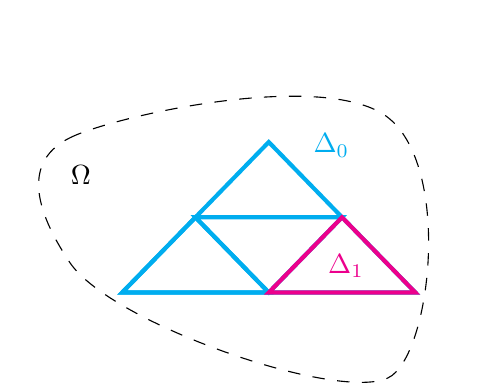
\begin{tikzpicture}[x=0.75pt,y=0.75pt,yscale=-1,xscale=1]
        %uncomment if require: \path (0,300); %set diagram left start at 0, and has height of 300
        
        %Shape: Triangle [id:dp00827622632180569] 
        \draw  [color=cyan  ,draw opacity=1 ][line width=1.5]  (170.63,87.51) -- (241.26,160) -- (100,160) -- cycle ;
        %Shape: Polygon Curved [id:ds3012264222748664] 
        \draw  [dash pattern={on 4.5pt off 4.5pt}] (74.74,85.49) .. controls (94.74,75.49) and (189,54) .. (224,73) .. controls (259,92) and (250,185) .. (230,200) .. controls (210,215) and (94.74,175.49) .. (74.74,145.49) .. controls (54.74,115.49) and (54.74,95.49) .. (74.74,85.49) -- cycle ;
        %Shape: Triangle [id:dp8224876385734627] 
        \draw  [color=cyan  ,draw opacity=1 ][line width=1.5]  (135.31,123.76) -- (170.63,160) -- (100,160) -- cycle ;
        %Shape: Triangle [id:dp8894284388389209] 
        \draw  [color=cyan  ,draw opacity=1 ][line width=1.5]  (170.63,160) -- (135.31,123.76) -- (205.94,123.76) -- cycle ;
        %Shape: Triangle [id:dp25960520730846914] 
        \draw  [color=magenta  ,draw opacity=1 ][line width=1.5]  (205.94,123.76) -- (241.26,160) -- (170.63,160) -- cycle ;
        
        % Text Node
        \draw (74,97.4) node [anchor=north west][inner sep=0.75pt]    {$\Omega $};
        % Text Node
        \draw (198,140.4) node [anchor=north west][inner sep=0.75pt]  [color=magenta  ,opacity=1 ]  {$\Delta _{1}$};
        % Text Node
        \draw (191,82.4) node [anchor=north west][inner sep=0.75pt]  [color=cyan  ,opacity=1 ]  {$\Delta _{0}$};
        
        
        \end{tikzpicture}
        \]
    By triangle inequality, \[|I|\leq \sum_{j=1}^{4}\left|\int_{\Delta_{0j}}f(z)\d z\right|\]
    Thus, there exists $j\in \{1,2,3,4\}$ such that \[\frac{|I|}{4}\leq \left|\int_{\Delta_{0j}}f(z)\d z\right|\]
    For this $j$, define $\Delta_1=\Delta_{0j}$.

    We disect $\Delta_1$ again into smaller triangles $\Delta_{1j}$ where $j=1,2,3,4$. Then, \[I=\int_{\Delta_1}f(z)\d z=\sum_{j=1}^{4}\int_{\Delta_{1j}}f(z)\d z\]
    Again, by triangle inequality, there is a $j\in \{1,2,3,4\}$ such that \[\rt{\frac{|I|}{4^2}}\leq \frac{1}{4}\left|\int_{\Delta_1}f(z)\d z\right|\leq \left|\int_{\Delta_{1j}}f(z)\d z\right|\]
    For this $j$, define $\Delta_2=\Delta_{1j}$.

    \[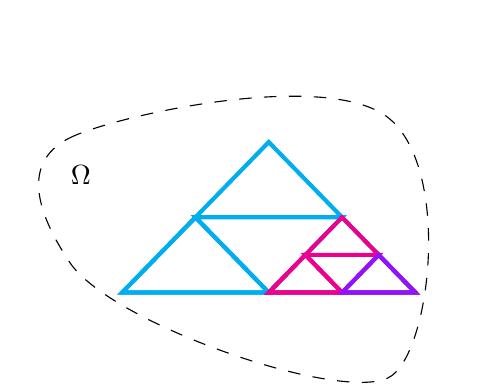
\begin{tikzpicture}[x=0.75pt,y=0.75pt,yscale=-1,xscale=1]
        %uncomment if require: \path (0,300); %set diagram left start at 0, and has height of 300
        
        %Shape: Triangle [id:dp00827622632180569] 
        \draw  [color=cyan  ,draw opacity=1 ][line width=1.5]  (170.63,87.51) -- (241.26,160) -- (100,160) -- cycle ;
        %Shape: Polygon Curved [id:ds3012264222748664] 
        \draw  [dash pattern={on 4.5pt off 4.5pt}] (74.74,85.49) .. controls (94.74,75.49) and (189,54) .. (224,73) .. controls (259,92) and (250,185) .. (230,200) .. controls (210,215) and (94.74,175.49) .. (74.74,145.49) .. controls (54.74,115.49) and (54.74,95.49) .. (74.74,85.49) -- cycle ;
        %Shape: Triangle [id:dp8224876385734627] 
        \draw  [color=cyan  ,draw opacity=1 ][line width=1.5]  (135.31,123.76) -- (170.63,160) -- (100,160) -- cycle ;
        %Shape: Triangle [id:dp8894284388389209] 
        \draw  [color=cyan  ,draw opacity=1 ][line width=1.5]  (170.63,160) -- (135.31,123.76) -- (205.94,123.76) -- cycle ;
        %Shape: Triangle [id:dp25960520730846914] 
        \draw  [color=magenta  ,draw opacity=1 ][line width=1.5]  (205.94,123.76) -- (241.26,160) -- (170.63,160) -- cycle ;
        %Shape: Triangle [id:dp9594922625539553] 
        \draw  [color=magenta  ,draw opacity=1 ][line width=1.5]  (188.28,141.88) -- (205.94,160) -- (170.63,160) -- cycle ;
        %Shape: Triangle [id:dp41273457544096503] 
        \draw  [color=magenta  ,draw opacity=1 ][line width=1.5]  (205.94,160) -- (188.28,141.88) -- (223.6,141.88) -- cycle ;
        %Shape: Triangle [id:dp4722169823972482] 
        \draw  [color={rgb, 255:red, 144; green, 19; blue, 254 }  ,draw opacity=1 ][line width=1.5]  (223.6,141.88) -- (241.26,160) -- (205.94,160) -- cycle ;
        
        % Text Node
        \draw (74,97.4) node [anchor=north west][inner sep=0.75pt]    {$\Omega $};
        
        
        \end{tikzpicture}        
        \]

    \dots continue in this manner to get nested triangles $\Delta_n$ such that \[\rt{\frac{|I|}{4^{n+1}}}\leq \frac{1}{4}\left|\int_{\Delta_n}f(z)\d z\right|\leq \left|\int_{\Delta_{nj}}f(z)\d z\right|\] for all $n\geq 0$.

    Now let $\ell=L(\Delta_0)$ denote perimeter of the original triangle (blue).\\ Then $L(\Delta_n)=\frac{\ell}{2^n}$\sidenote{Perimeter of $\Delta_n$}. 

    Let $K_n$ denote the triangle $\Delta_n$ union with its interior such that $K_n$ is closed (in fact, compact!). Let $\zeta_n\in K_n$ for $n\geq 0$. Then there is $N\in \N$, such that for all $m,n\geq N$ we have $|\zeta_m-\zeta_n|\leq \operatorname{diam}(K_N)\leq \frac{\ell}{2^N}$. Thus, $\zeta_n$ as a sequence is Cauchy.

    Let $z_0=\lim_{n\to\infty}\zeta_n$, note $z_0\in \bigcap_{n=0}^{\infty} K_n$ and $z_0\in \Omega$. Since $f$ is analytic at $z_0$, given $\varepsilon>0$, there exists some $\delta>0$ such that whenever $|z-z_0|<\delta$, we have \[\left|\frac{f(z)-f(z_0)}{z-z_0}-f'(z_0)\right|<\frac{\varepsilon}{\ell^2}\]

    Now consider multiplying $|z-z_0|$ on both sides:
    \begin{align*}
        |f'(z_0)\cdot (z-z_0) - f(z) + f(z_0)| &< \frac{\varepsilon}{\ell^2} |z-z_0|\\
        |f(z_0) + f'(z_0)(z-z_0)-f(z)| &<\frac{\varepsilon}{\ell^2} |z-z_0|
    \end{align*}
    Since $f(z_0) + f'(z_0)(z-z_0)$ is \textbf{linear}, it has an antiderivative on $\C$. Thus, \[\int_{\Delta_n}f(z_0) + f'(z_0)(z-z_0)\d z = 0\]
    by FTC! Now pick $n$ large enough so that $|z-z_0<\delta$ for all $z\in \Delta_n$. Thus, \begin{align*}
        |I|&\leq 4^n \left|\int_{\Delta_n}f(z)\d z\right|\\ 
        &= 4^n\left|\int_{\Delta_n}f(z_0) + f'(z_0)(z-z_0)-f(z)\right|\\
        &\leq 4^n\frac{\varepsilon}{\ell^2}|z-z_0|\frac{\ell}{2^n} &&\text{by tri. ineq. and }\left|\int_\gamma g(z)\d z\right|\leq \sup_{z\in \gamma}|g(z)|\cdot L(\gamma)\\
        &< \frac{4^n\varepsilon}{\ell 2^n}\cdot \frac{\ell}{2^n}\\
        &= \varepsilon
    \end{align*}

   
\end{proof}

\subsubsection{Local antiderivative}
\begin{theorem}\label[theorem]{convex-antiderivative}
    If $\reg$ is convex and $f:\reg \to \C$ is analytic, then $f$ has an antiderivative on $\reg$.
\end{theorem}
\rmk Line segments don't exit the region in convex shapes:\[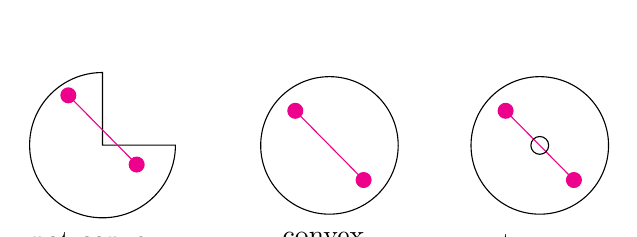
\begin{tikzpicture}[x=0.75pt,y=0.75pt,yscale=-1,xscale=1]
    %uncomment if require: \path (0,300); %set diagram left start at 0, and has height of 300
    
    %Shape: Pie [id:dp6860240797492949] 
    \draw   (136.92,115.67) .. controls (136.92,115.67) and (136.92,115.67) .. (136.92,115.67) .. controls (136.92,135) and (121.19,150.67) .. (101.79,150.67) .. controls (82.39,150.67) and (66.67,135) .. (66.67,115.67) .. controls (66.67,96.34) and (82.39,80.67) .. (101.79,80.67) -- (101.79,115.67) -- cycle ;
    %Straight Lines [id:da6856373582050304] 
    \draw [color=magenta  ,draw opacity=1 ]   (85.33,91.67) -- (118.25,125.01) ;
    \draw [shift={(118.25,125.01)}, rotate = 45.36] [color=magenta  ,draw opacity=1 ][fill=magenta  ,fill opacity=1 ][line width=0.75]      (0, 0) circle [x radius= 3.35, y radius= 3.35]   ;
    \draw [shift={(85.33,91.67)}, rotate = 45.36] [color=magenta  ,draw opacity=1 ][fill=magenta  ,fill opacity=1 ][line width=0.75]      (0, 0) circle [x radius= 3.35, y radius= 3.35]   ;
    %Shape: Circle [id:dp6630767252853171] 
    \draw   (178,115.79) .. controls (178,97.5) and (192.83,82.67) .. (211.13,82.67) .. controls (229.42,82.67) and (244.25,97.5) .. (244.25,115.79) .. controls (244.25,134.09) and (229.42,148.92) .. (211.13,148.92) .. controls (192.83,148.92) and (178,134.09) .. (178,115.79) -- cycle ;
    %Shape: Circle [id:dp7587345978022606] 
    \draw   (279.33,115.79) .. controls (279.33,97.5) and (294.16,82.67) .. (312.46,82.67) .. controls (330.76,82.67) and (345.59,97.5) .. (345.59,115.79) .. controls (345.59,134.09) and (330.76,148.92) .. (312.46,148.92) .. controls (294.16,148.92) and (279.33,134.09) .. (279.33,115.79) -- cycle ;
    %Straight Lines [id:da09760158868609392] 
    \draw [color=magenta  ,draw opacity=1 ]   (194.67,99.12) -- (227.59,132.47) ;
    \draw [shift={(227.59,132.47)}, rotate = 45.36] [color=magenta  ,draw opacity=1 ][fill=magenta  ,fill opacity=1 ][line width=0.75]      (0, 0) circle [x radius= 3.35, y radius= 3.35]   ;
    \draw [shift={(194.67,99.12)}, rotate = 45.36] [color=magenta  ,draw opacity=1 ][fill=magenta  ,fill opacity=1 ][line width=0.75]      (0, 0) circle [x radius= 3.35, y radius= 3.35]   ;
    %Straight Lines [id:da4239725771757499] 
    \draw [color=magenta  ,draw opacity=1 ]   (296,99.12) -- (328.92,132.47) ;
    \draw [shift={(328.92,132.47)}, rotate = 45.36] [color=magenta  ,draw opacity=1 ][fill=magenta  ,fill opacity=1 ][line width=0.75]      (0, 0) circle [x radius= 3.35, y radius= 3.35]   ;
    \draw [shift={(296,99.12)}, rotate = 45.36] [color=magenta  ,draw opacity=1 ][fill=magenta  ,fill opacity=1 ][line width=0.75]      (0, 0) circle [x radius= 3.35, y radius= 3.35]   ;
    %Shape: Circle [id:dp6744384543792539] 
    \draw   (308.17,115.79) .. controls (308.17,113.43) and (310.09,111.5) .. (312.46,111.5) .. controls (314.83,111.5) and (316.75,113.43) .. (316.75,115.79) .. controls (316.75,118.16) and (314.83,120.08) .. (312.46,120.08) .. controls (310.09,120.08) and (308.17,118.16) .. (308.17,115.79) -- cycle ;
    
    % Text Node
    \draw (66,156.67) node [anchor=north west][inner sep=0.75pt]   [align=left] {not convex};
    % Text Node
    \draw (187.33,156.67) node [anchor=north west][inner sep=0.75pt]   [align=left] {convex};
    % Text Node
    \draw (278.67,157.33) node [anchor=north west][inner sep=0.75pt]   [align=left] {not convex};
    
    
    \end{tikzpicture}
    \]
\begin{proof}
    Fix $w\in \reg$ and define: \[F(z)=\int_{[w,z]}f(\zeta)\d \zeta\] for $z\in \reg$.\sidenote{$[w,z]$ is the line segment from $w$ to $z$.}

    This is well-defined if $\reg$ is convex.

    Now we \dashuline{want to show} that $F'$ is $f$. That is equivalent to showing that for all $\varepsilon>0, z_0\in \reg$, there exists $\delta>0$ s.t. whenever $|z-z_0|<\delta$, we have  \[\left|\frac{F(z)-F(z_0)}{z-z_0}-f(z_0)\right|<{\varepsilon}\]
    Let $z_0\in \Omega$ be given and $\varepsilon>0$. Goursat says integrals around the triangle is 0, so we suppose $z\in \reg\backslash\{z_0,w\}$ and get a triangle:
    \[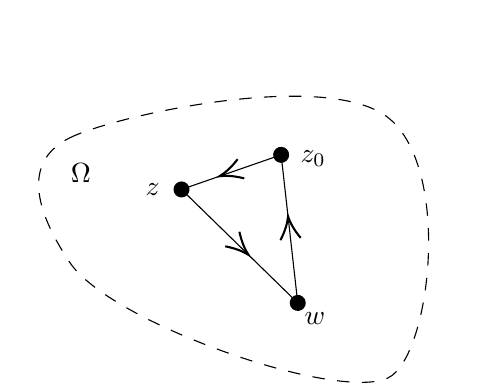
\begin{tikzpicture}[x=0.75pt,y=0.75pt,yscale=-1,xscale=1]
        %uncomment if require: \path (0,300); %set diagram left start at 0, and has height of 300
        
        %Shape: Polygon Curved [id:ds8013551056257879] 
        \draw  [dash pattern={on 4.5pt off 4.5pt}] (94.74,106.15) .. controls (114.74,96.15) and (209,74.67) .. (244,93.67) .. controls (279,112.67) and (270,205.67) .. (250,220.67) .. controls (230,235.67) and (114.74,196.15) .. (94.74,166.15) .. controls (74.74,136.15) and (74.74,116.15) .. (94.74,106.15) -- cycle ;
        %Straight Lines [id:da8523806034462806] 
        \draw    (148.59,131.01) -- (204.59,185.68) ;
        \draw [shift={(180.88,162.53)}, rotate = 224.31] [color=black  ][line width=0.75]    (10.93,-4.9) .. controls (6.95,-2.3) and (3.31,-0.67) .. (0,0) .. controls (3.31,0.67) and (6.95,2.3) .. (10.93,4.9)   ;
        \draw [shift={(148.59,131.01)}, rotate = 44.31] [color=black  ][fill=black  ][line width=0.75]      (0, 0) circle [x radius= 3.35, y radius= 3.35]   ;
        %Straight Lines [id:da16858040739980074] 
        \draw    (204.59,185.68) -- (196.59,114.34) ;
        \draw [shift={(199.92,144.05)}, rotate = 83.6] [color=black  ][line width=0.75]    (10.93,-4.9) .. controls (6.95,-2.3) and (3.31,-0.67) .. (0,0) .. controls (3.31,0.67) and (6.95,2.3) .. (10.93,4.9)   ;
        \draw [shift={(204.59,185.68)}, rotate = 263.6] [color=black  ][fill=black  ][line width=0.75]      (0, 0) circle [x radius= 3.35, y radius= 3.35]   ;
        %Straight Lines [id:da12021387715434817] 
        \draw    (196.59,114.34) -- (148.59,131.01) ;
        \draw [shift={(166.92,124.64)}, rotate = 340.85] [color=black  ][line width=0.75]    (10.93,-4.9) .. controls (6.95,-2.3) and (3.31,-0.67) .. (0,0) .. controls (3.31,0.67) and (6.95,2.3) .. (10.93,4.9)   ;
        \draw [shift={(196.59,114.34)}, rotate = 160.85] [color=black  ][fill=black  ][line width=0.75]      (0, 0) circle [x radius= 3.35, y radius= 3.35]   ;
        
        % Text Node
        \draw (94,117.4) node [anchor=north west][inner sep=0.75pt]    {$\Omega $};
        % Text Node
        \draw (130,127.07) node [anchor=north west][inner sep=0.75pt]    {$z$};
        % Text Node
        \draw (204.67,111.07) node [anchor=north west][inner sep=0.75pt]    {$z_{0}$};
        % Text Node
        \draw (206.59,189.08) node [anchor=north west][inner sep=0.75pt]    {$w$};
        
        
        \end{tikzpicture}
        \]
        and we know that \[\underset{F(z_0)}{\underbrace{\int_{[w,z_0]}f(\zeta)\d \zeta}} + \int_{[z_0,z]}f(\zeta)\d \zeta + \underset{-F(z)}{\underbrace{\int_{[z,w]}f(\zeta)\d \zeta}}=0\]
        So $F(z)-F(z_0)=\int_{[z_0,z]}f(\zeta)\d \zeta$. Thus,
        \begin{align*}
            \frac{F(z)-F(z_0)}{z-z_0}\rt{-f(z_0)} &= \frac{1}{z-z_0}\int_{[z_0,z]}\left(f(\zeta)-f(z_0)\right)\d \zeta
        \end{align*}
        Since $f$ is analytic at $z_0$, it is continuous there. Given $\varepsilon>0$, there exists $\delta>0$ such that whenever $|z-z_0|<\delta$, we have  \(\left|f(z)-f(z_0)\right|<{\varepsilon}\).

        Therefore, whenever $|z-z_0|<\delta$, we have \sidenote{still by \(\left|\int_\gamma g(z)\d z\right|\leq \sup_{z\in \gamma}|g(z)|\cdot L(\gamma)\)}\begin{align*}
            \left|\frac{F(z)-F(z_0)}{z-z_0}-f(z_0)\right| &\leq \frac{\varepsilon}{|z-z_0|}L([z_0,z])\\
            &= \frac{\varepsilon}{|z-z_0|}|z-z_0|\\
            &= \varepsilon
        \end{align*}
\end{proof}

\subsection{Cauchy's theorem, Take 3}
\subsubsection{Cauchy's theorem for convex regions}
\begin{theorem}
    If $\reg$ is convex, $f:\reg\to \C$ analytic and $\gamma$ is a piecewise $C^1$ curve in $\reg$, then $\int_{\gamma}f(z)\d z=0$.\sidenote{Since $\reg$ is convex, the interior of $\gamma$ lies inside $\reg$.}
\end{theorem}
\begin{proof}
    Previous theorem says $f$ has an antiderivative $F$ on $\reg$. Thus, \[\int_{\gamma}f(z)\d z = \int_{\gamma}F'(z)\d z=0\] by FTC!
\end{proof}

\subsection{Cauchy's integral formula}
\subsubsection{Cauchy's integral formula for a circle}
\hypertarget{cauchys-integral-formula}{}
\begin{theorem}\label[theorem]{cif}
    If $f$ is analytic on a region $\Omega$ that contains the circle $\gamma$ and its interior, then \[f(z)=\frac{1}{2\pi i}\int_{\gamma}\frac{f(\zeta)\d \zeta}{\zeta-z}\] for all $z$ inside of $\gamma$.\sidenote{this $\reg$ doesn't need to be convex}
\end{theorem}
\begin{proof}
    Let $r>0$ be small enough so that the closed ball $B_r(z)^-$ is in the interior of $\gamma$. Let $C_r(z)=\{\zeta\in\C :|\zeta-z|=r\}$ traversed clockwise.
    \[\begin{tikzpicture}[x=0.75pt,y=0.75pt,yscale=-0.75,xscale=0.75]
        %uncomment if require: \path (0,300); %set diagram left start at 0, and has height of 300
        
        %Shape: Polygon Curved [id:ds2869580135529062] 
        \draw  [dash pattern={on 4.5pt off 4.5pt}] (85.36,55.55) .. controls (125.83,35.31) and (316.58,-8.17) .. (387.41,30.28) .. controls (458.25,68.73) and (440.03,256.94) .. (399.56,287.29) .. controls (359.08,317.65) and (125.83,237.68) .. (85.36,176.97) .. controls (44.88,116.26) and (44.88,75.78) .. (85.36,55.55) -- cycle ;
        %Shape: Ellipse [id:dp5518722967005327] 
        \draw   (198.69,145.86) .. controls (198.69,93.75) and (240.93,51.5) .. (293.05,51.5) .. controls (345.17,51.5) and (387.41,93.75) .. (387.41,145.86) .. controls (387.41,197.98) and (345.17,240.23) .. (293.05,240.23) .. controls (240.93,240.23) and (198.69,197.98) .. (198.69,145.86) -- cycle ;
        %Shape: Arc [id:dp14115450919361172] 
        \draw  [draw opacity=0] (362.61,130.43) .. controls (362.61,158.37) and (339.96,181.02) .. (312.02,181.02) .. controls (284.07,181.02) and (261.42,158.37) .. (261.42,130.43) .. controls (261.42,102.48) and (284.07,79.83) .. (312.02,79.83) .. controls (339.66,79.83) and (362.13,102.01) .. (362.6,129.54) -- (312.02,130.43) -- cycle ; \draw    (362.61,130.43) .. controls (362.61,158.37) and (339.96,181.02) .. (312.02,181.02) .. controls (284.07,181.02) and (261.42,158.37) .. (261.42,130.43) .. controls (261.42,102.48) and (284.07,79.83) .. (312.02,79.83) .. controls (339.11,79.83) and (361.23,101.13) .. (362.55,127.9) ; \draw [shift={(362.6,129.54)}, rotate = 269.02] [color=black  ][line width=0.75]    (10.93,-3.29) .. controls (6.95,-1.4) and (3.31,-0.3) .. (0,0) .. controls (3.31,0.3) and (6.95,1.4) .. (10.93,3.29)   ; 
        %Straight Lines [id:da08707833068540416] 
        \draw    (312.02,79.83) -- (312.02,130.43) ;
        \draw [shift={(312.02,130.43)}, rotate = 90] [color=black  ][fill=black  ][line width=0.75]      (0, 0) circle [x radius= 3.35, y radius= 3.35]   ;
        
        % Text Node
        \draw (79.38,84.37) node [anchor=north west][inner sep=0.75pt]    {$\Omega $};
        % Text Node
        \draw (196.73,60.09) node [anchor=north west][inner sep=0.75pt]    {$\gamma $};
        % Text Node
        \draw (322.21,145.09) node [anchor=north west][inner sep=0.75pt]    {$z$};
        % Text Node
        \draw (300.95,99.47) node [anchor=north west][inner sep=0.75pt]    {$r$};
        
        
        \end{tikzpicture}
        \]

        Construct $\gamma_1,\gamma_2,\gamma_3,\gamma_4$ as pictured:
        \[\begin{tikzpicture}[x=0.75pt,y=0.75pt,yscale=-1,xscale=1]
            %uncomment if require: \path (0,300); %set diagram left start at 0, and has height of 300
            
            %Shape: Polygon Curved [id:ds2869580135529062] 
            \draw  [dash pattern={on 4.5pt off 4.5pt}] (85.36,55.55) .. controls (125.83,35.31) and (316.58,-8.17) .. (387.41,30.28) .. controls (458.25,68.73) and (440.03,256.94) .. (399.56,287.29) .. controls (359.08,317.65) and (125.83,237.68) .. (85.36,176.97) .. controls (44.88,116.26) and (44.88,75.78) .. (85.36,55.55) -- cycle ;
            %Shape: Arc [id:dp4628794505771803] 
            \draw  [draw opacity=0] (387.41,145.86) .. controls (387.41,145.86) and (387.41,145.86) .. (387.41,145.86) .. controls (387.41,197.98) and (345.17,240.23) .. (293.05,240.23) .. controls (240.93,240.23) and (198.69,197.98) .. (198.69,145.86) .. controls (198.69,93.75) and (240.93,51.5) .. (293.05,51.5) .. controls (344.62,51.5) and (386.52,92.86) .. (387.4,144.22) -- (293.05,145.86) -- cycle ; \draw    (387.41,145.86) .. controls (387.41,197.98) and (345.17,240.23) .. (293.05,240.23) .. controls (240.93,240.23) and (198.69,197.98) .. (198.69,145.86) .. controls (198.69,93.75) and (240.93,51.5) .. (293.05,51.5) .. controls (344.62,51.5) and (386.52,92.86) .. (387.4,144.22) ;  \draw [shift={(387.41,145.86)}, rotate = 90] [color=black  ][line width=0.75]    (10.93,-4.9) .. controls (6.95,-2.3) and (3.31,-0.67) .. (0,0) .. controls (3.31,0.67) and (6.95,2.3) .. (10.93,4.9)   ;
            %Shape: Arc [id:dp14115450919361172] 
            \draw  [draw opacity=0] (362.61,130.43) .. controls (362.61,158.37) and (339.96,181.02) .. (312.02,181.02) .. controls (284.07,181.02) and (261.42,158.37) .. (261.42,130.43) .. controls (261.42,102.48) and (284.07,79.83) .. (312.02,79.83) .. controls (339.66,79.83) and (362.13,102.01) .. (362.6,129.54) -- (312.02,130.43) -- cycle ; \draw    (362.61,130.43) .. controls (362.61,158.37) and (339.96,181.02) .. (312.02,181.02) .. controls (284.07,181.02) and (261.42,158.37) .. (261.42,130.43) .. controls (261.42,102.48) and (284.07,79.83) .. (312.02,79.83) .. controls (339.11,79.83) and (361.23,101.13) .. (362.55,127.9) ; \draw [shift={(362.6,129.54)}, rotate = 269.02] [color=black  ][line width=0.75]    (10.93,-3.29) .. controls (6.95,-1.4) and (3.31,-0.3) .. (0,0) .. controls (3.31,0.3) and (6.95,1.4) .. (10.93,3.29)   ; 
            %Straight Lines [id:da08707833068540416] 
            \draw    (312.02,79.83) -- (312.02,130.43) ;
            \draw [shift={(312.02,130.43)}, rotate = 90] [color=black  ][fill=black  ][line width=0.75]      (0, 0) circle [x radius= 3.35, y radius= 3.35]   ;
            %Straight Lines [id:da42001019106573523] 
            \draw    (199.26,146) -- (264.26,146) ;
            %Straight Lines [id:da5050562029853729] 
            \draw    (360.26,145.86) -- (387.41,145.86) ;
            %Straight Lines [id:da6466886705419264] 
            \draw    (302,52) -- (302,80.26) ;
            %Straight Lines [id:da5525798176108874] 
            \draw    (302,180) -- (302,239.26) ;
            %Shape: Arc [id:dp6786536818536373] 
            \draw  [draw opacity=0] (252.12,206.17) .. controls (253.6,206.71) and (255.2,207) .. (256.87,207) .. controls (264.53,207) and (270.74,200.79) .. (270.74,193.13) .. controls (270.74,185.47) and (264.53,179.26) .. (256.87,179.26) .. controls (249.21,179.26) and (243,185.47) .. (243,193.13) .. controls (243,193.44) and (243.01,193.74) .. (243.03,194.05) -- (256.87,193.13) -- cycle ; \draw    (252.12,206.17) .. controls (253.6,206.71) and (255.2,207) .. (256.87,207) .. controls (264.53,207) and (270.74,200.79) .. (270.74,193.13) .. controls (270.74,185.47) and (264.53,179.26) .. (256.87,179.26) .. controls (249.21,179.26) and (243,185.47) .. (243,193.13) ; \draw [shift={(243.03,194.05)}, rotate = 291.14] [color=black  ][line width=0.75]    (10.93,-3.29) .. controls (6.95,-1.4) and (3.31,-0.3) .. (0,0) .. controls (3.31,0.3) and (6.95,1.4) .. (10.93,3.29)   ; 
            %Shape: Arc [id:dp5061770598860282] 
            \draw  [draw opacity=0] (334.12,211.17) .. controls (335.6,211.71) and (337.2,212) .. (338.87,212) .. controls (346.53,212) and (352.74,205.79) .. (352.74,198.13) .. controls (352.74,190.47) and (346.53,184.26) .. (338.87,184.26) .. controls (331.21,184.26) and (325,190.47) .. (325,198.13) .. controls (325,198.44) and (325.01,198.74) .. (325.03,199.05) -- (338.87,198.13) -- cycle ; \draw    (334.12,211.17) .. controls (335.6,211.71) and (337.2,212) .. (338.87,212) .. controls (346.53,212) and (352.74,205.79) .. (352.74,198.13) .. controls (352.74,190.47) and (346.53,184.26) .. (338.87,184.26) .. controls (331.21,184.26) and (325,190.47) .. (325,198.13) ; \draw [shift={(325.03,199.05)}, rotate = 291.14] [color=black  ][line width=0.75]    (10.93,-3.29) .. controls (6.95,-1.4) and (3.31,-0.3) .. (0,0) .. controls (3.31,0.3) and (6.95,1.4) .. (10.93,3.29)   ; 
            %Shape: Arc [id:dp2571796670898707] 
            \draw  [draw opacity=0] (234.12,129.17) .. controls (235.6,129.71) and (237.2,130) .. (238.87,130) .. controls (246.53,130) and (252.74,123.79) .. (252.74,116.13) .. controls (252.74,108.47) and (246.53,102.26) .. (238.87,102.26) .. controls (231.21,102.26) and (225,108.47) .. (225,116.13) .. controls (225,116.44) and (225.01,116.74) .. (225.03,117.05) -- (238.87,116.13) -- cycle ; \draw    (234.12,129.17) .. controls (235.6,129.71) and (237.2,130) .. (238.87,130) .. controls (246.53,130) and (252.74,123.79) .. (252.74,116.13) .. controls (252.74,108.47) and (246.53,102.26) .. (238.87,102.26) .. controls (231.21,102.26) and (225,108.47) .. (225,116.13) ; \draw [shift={(225.03,117.05)}, rotate = 291.14] [color=black  ][line width=0.75]    (10.93,-3.29) .. controls (6.95,-1.4) and (3.31,-0.3) .. (0,0) .. controls (3.31,0.3) and (6.95,1.4) .. (10.93,3.29)   ; 
            %Shape: Arc [id:dp9245710959560463] 
            \draw  [draw opacity=0] (318.16,77.44) .. controls (319.16,77.8) and (320.24,78) .. (321.37,78) .. controls (326.54,78) and (330.74,73.81) .. (330.74,68.63) .. controls (330.74,63.46) and (326.54,59.26) .. (321.37,59.26) .. controls (316.19,59.26) and (312,63.46) .. (312,68.63) .. controls (312,68.84) and (312.01,69.05) .. (312.02,69.25) -- (321.37,68.63) -- cycle ; \draw    (318.16,77.44) .. controls (319.16,77.8) and (320.24,78) .. (321.37,78) .. controls (326.54,78) and (330.74,73.81) .. (330.74,68.63) .. controls (330.74,63.46) and (326.54,59.26) .. (321.37,59.26) .. controls (316.19,59.26) and (312,63.46) .. (312,68.63) ; \draw [shift={(312.02,69.25)}, rotate = 302.63] [color=black  ][line width=0.75]    (10.93,-3.29) .. controls (6.95,-1.4) and (3.31,-0.3) .. (0,0) .. controls (3.31,0.3) and (6.95,1.4) .. (10.93,3.29)   ; 
            
            % Text Node
            \draw (79.38,84.37) node [anchor=north west][inner sep=0.75pt]    {$\Omega $};
            % Text Node
            \draw (196.73,59.09) node [anchor=north west][inner sep=0.75pt]    {$\gamma _{2}$};
            % Text Node
            \draw (322.21,145.09) node [anchor=north west][inner sep=0.75pt]    {$z$};
            % Text Node
            \draw (300.95,99.47) node [anchor=north west][inner sep=0.75pt]    {$r$};
            % Text Node
            \draw (351.73,44.09) node [anchor=north west][inner sep=0.75pt]    {$\gamma _{1}$};
            % Text Node
            \draw (188.73,195.09) node [anchor=north west][inner sep=0.75pt]    {$\gamma _{3}$};
            % Text Node
            \draw (379.73,208.09) node [anchor=north west][inner sep=0.75pt]    {$\gamma _{4}$};
            
            
            \end{tikzpicture}
            \]
            Cauchy's theorem for convex regions says $\int_{\gamma_i}\frac{f(\zeta)\d \zeta}{\zeta-z}=0$ for all $i=1,2,3,4$.

            Hence, \[0=\sum_{j=1}^{4}\int_{\gamma_j}\frac{f(\zeta)\d \zeta}{\zeta-z}=\rt{
                \int_{\gamma}\frac{f(\zeta)\d \zeta}{\zeta-z} - \int_{C_r(z)}\frac{f(\zeta)\d \zeta}{\zeta-z}
            }\]

            And thus: \[ \int_{\gamma}\frac{f(\zeta)\d \zeta}{\zeta-z}= \int_{C_r(z)}\frac{f(\zeta)\d \zeta}{\zeta-z}\] for all $r>0$ that is \textit{sufficiently} small.

            Therefore:\sidenote{\rt{by HW6 Ex5, or Thm12 Lect 11}} \begin{align*}
                \left|\frac{1}{2\pi i} \int_{\bt{\gamma}}\frac{f(\zeta)\d \zeta}{\zeta-z}-f(z)\cdot \rt{1}\right| &=  \left|\frac{1}{2\pi i} \int_{\bt{\gamma}}\frac{f(\zeta)\d \zeta}{\zeta-z}-f(z)\cdot \rt{\left(\frac{1}{2\pi i}\int_{C_r(z)}\frac{\d \zeta}{\zeta-z}\right)}\right|\\
                &= \left|\frac{1}{2\pi i} \int_{\bt{C_r(z)}}\frac{f(\zeta)\d \zeta}{\zeta-z}-f(z)\cdot \rt{\left(\frac{1}{2\pi i}\int_{C_r(z)}\frac{\d \zeta}{\zeta-z}\right)}\right|\\
                &= \lim_{r\to 0^+}\left|\frac{1}{2\pi i}\int_{C_r(z)}\frac{f(\zeta)-f(z)}{\zeta-z}\right|\\
                &\leq \gt{\lim_{r\to 0^+}} \max_{|\zeta-z|=r}\left|\frac{f(\zeta)-f(z)}{\zeta-z}\right|\cdot \gt{r}\\
                &= 0
            \end{align*}
\end{proof}

\subsubsection{Mean value properties}
\begin{corollary}[Mean value property for analytic functions]
    If $f$ analytic on an open set $\reg$ which contains $B_r(z)^-$, then \[f(z)=\frac{1}{2\pi}\int_{0}^{2\pi}f(z+re^{it})\d t\]
\end{corollary}
\begin{proof}
    Apply \cref{cif} with $\zeta=z+re^{it}$ and $\d \zeta=ire^{it}\d t, t\in [0,2\pi]$ and get \begin{align*}
        f(z)&= \frac{1}{2\pi i}\int_{C_r(z)}\frac{f(\zeta)\d \zeta}{\zeta-z}\\
        &= \frac{1}{2\pi i}\int_{C_r(z)}\frac{f(z+re^{it})ire^{it}\d t}{z+re^{it}-z}\\
        &= \frac{1}{2\pi}\int_{0}^{2\pi}f(z+re^{it})\d t
    \end{align*}
\end{proof}

\rmk There is a mean value property for harmonic functions!

\subsection{Existence of power series expansions}
\begin{theorem}
    If $f:\reg\to\C$ is analytic and $z_0\in \reg$ then $f$ has a power series expansions \[f(z)=\sum_{n=0}^{\infty}a_n(z-z_0)^n\] that converges \textbf{locally uniformly} on the disk \[|z-z_0|<\operatorname{dist}(z_0, \reg^C)= \inf_{w\in \reg^C}|z_0-w|\] when $\reg^C$ is nonempty.\sidenote{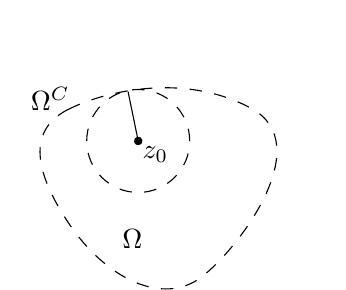
\begin{tikzpicture}[x=0.75pt,y=0.75pt,yscale=-0.45,xscale=0.45]
        %uncomment if require: \path (0,300); %set diagram left start at 0, and has height of 300
        
        %Shape: Polygon Curved [id:ds75764139255783] 
        \draw  [dash pattern={on 4.5pt off 4.5pt}] (105.36,58.25) .. controls (145.83,38.01) and (230.42,18.81) .. (301.26,57.26) .. controls (372.09,95.72) and (287.73,207.91) .. (247.26,238.26) .. controls (206.78,268.62) and (145.83,240.39) .. (105.36,179.68) .. controls (64.88,118.96) and (64.88,78.49) .. (105.36,58.25) -- cycle ;
        %Shape: Circle [id:dp1108533721802123] 
        \draw  [dash pattern={on 4.5pt off 4.5pt}] (125,92.13) .. controls (125,61.68) and (149.68,37) .. (180.13,37) .. controls (210.57,37) and (235.26,61.68) .. (235.26,92.13) .. controls (235.26,122.57) and (210.57,147.26) .. (180.13,147.26) .. controls (149.68,147.26) and (125,122.57) .. (125,92.13) -- cycle ;
        %Straight Lines [id:da9925386809993804] 
        \draw    (169.26,39.26) -- (180.13,92.13) ;
        \draw [shift={(180.13,92.13)}, rotate = 78.38] [color=black  ][fill=black  ][line width=0.75]      (0, 0) circle [x radius= 3.35, y radius= 3.35]   ;
        
        % Text Node
        \draw (160.38,184.08) node [anchor=north west][inner sep=0.75pt]    {$\Omega $};
        % Text Node
        \draw (62.38,32.08) node [anchor=north west][inner sep=0.75pt]    {$\Omega ^{C}$};
        % Text Node
        \draw (182.13,95.53) node [anchor=north west][inner sep=0.75pt]    {$z_{0}$};
        
        
        \end{tikzpicture}
        }

    Moreover, the radius of convergence is the radius of the largest open disk centered at $z_0$ upon which $f$ could be analytically continued.
\end{theorem}

\begin{proof}
    Let $r<\operatorname*{dist}(z_0,\reg^C)$ and $|z-z_0|\leq \rho<r$. Then \[f(z)=\frac{1}{2\pi i} \int_{{C_r(z_0)}}\frac{f(\zeta)\d \zeta}{\zeta-z}\] for all $|z-z_0|<\rho$. 

    As a function of $\zeta$, the series\sidenote{geometric series trick!} \[\frac{1}{\zeta-z}=\frac{1}{(\zeta-z_0)-(z-z_0)}=\frac{1}{\zeta-z_0}\cdot \frac{1}{1-\frac{z-z_0}{\zeta-z_0}}\]
    and so by geometric series formula:
    \begin{align*}
        \frac{1}{\zeta-z} &= \frac{1}{\zeta-z_0}\sum_{n=0}^{\infty}\left(\frac{z-z_0}{\zeta-z_0}\right)^n\\
        &= \sum_{n=0}^{\infty}\frac{(z-z_0)^n}{(\zeta-z_0)^{n+1}} &&\text{for } |z-z_0|\leq \rho
    \end{align*}
    converges uniformly on $|\zeta-z_0|=r$ by the Weierstrass M-test with $M_n=\left|\frac{z-z_0}{\zeta-z_0}\right|^n\leq \left(\frac{\rho}{r}\right)^n$.

    Thus, \begin{align*}
        f(z)&=\frac{1}{2\pi i}\int_{{C_r(z_0)}}\frac{f(\zeta)\d \zeta}{\zeta-z}\\
        &= \frac{1}{2\pi i}\int_{{C_r(z_0)}}\rt{\sum_{n=0}^{\infty}\frac{(z-z_0)^n}{(\zeta-z_0)^{n+1}}}\cdot f(\zeta)\d \zeta\\
        &= \sum_{n=0}^{\infty}(z-z_0)^n\bt{
            \frac{1}{2\pi i}\int_{{C_r(z_0)}}\frac{f(\zeta)\d \zeta}{(\zeta-z_0)^{n+1}}
        }
    \end{align*}
    And so we have our $\bt{\frac{f^{(n)}(z_0)}{n!}=a_n}$ in the highlighted part above. 
\end{proof}

\rmk Consequently, we also get Cauchy's theorem of derivatives: \[f^{(n)}(z_0) = \frac{n!}{2\pi i}\int_{{C_r(z_0)}}\frac{f(\zeta)\d \zeta}{(\zeta-z_0)^{n+1}}\]

\eg What is the radius of convergence for the power series of \[f(x)=\frac{e^{\sin x}+e^{-x^2}+x^2+7x^3}{\cos x}\] centered at $x_0=2$?

The theorem guarantees the existence of the power series, and the RoC would simply be the radius of which $f$ could be analytically continued. We observe that $f(x)$ cannot be defined when $\cos x=0$, i.e. $x=\frac{\pi}{2}$. Hence, the radius of convergence is just $2-\frac{\pi}{2}$ -- no need to compute \textit{any} derivatives or coefficients!

\spl

So now we have this result for computing the derivatives and integrals around a circle $C_r(z_0)$. Can we extend this to other closed curves of any shapes?

\[\begin{tikzpicture}[x=0.75pt,y=0.75pt,yscale=-1,xscale=1]
    %uncomment if require: \path (0,300); %set diagram left start at 0, and has height of 300
    
    %Curve Lines [id:da21494767258082992] 
    \draw    (202.26,132.76) .. controls (260.26,132.76) and (232.42,21.55) .. (303.26,60) .. controls (374.09,98.45) and (424.73,204.41) .. (384.26,234.76) .. controls (343.78,265.12) and (293.26,262.76) .. (245.26,241.76) .. controls (197.26,220.76) and (104.26,255.76) .. (80.26,215.76) .. controls (56.26,175.76) and (161.26,132.51) .. (202.26,132.76) -- cycle ;
    \draw [shift={(250.18,76.55)}, rotate = 112.47] [color=black  ][line width=0.75]    (10.93,-4.9) .. controls (6.95,-2.3) and (3.31,-0.67) .. (0,0) .. controls (3.31,0.67) and (6.95,2.3) .. (10.93,4.9)   ;
    \draw [shift={(380.72,140.93)}, rotate = 240.89] [color=black  ][line width=0.75]    (10.93,-4.9) .. controls (6.95,-2.3) and (3.31,-0.67) .. (0,0) .. controls (3.31,0.67) and (6.95,2.3) .. (10.93,4.9)   ;
    \draw [shift={(309.73,257.48)}, rotate = 0.74] [color=black  ][line width=0.75]    (10.93,-4.9) .. controls (6.95,-2.3) and (3.31,-0.67) .. (0,0) .. controls (3.31,0.67) and (6.95,2.3) .. (10.93,4.9)   ;
    \draw [shift={(153.76,235.89)}, rotate = 357.8] [color=black  ][line width=0.75]    (10.93,-4.9) .. controls (6.95,-2.3) and (3.31,-0.67) .. (0,0) .. controls (3.31,0.67) and (6.95,2.3) .. (10.93,4.9)   ;
    \draw [shift={(129.21,152.85)}, rotate = 153.94] [color=black  ][line width=0.75]    (10.93,-4.9) .. controls (6.95,-2.3) and (3.31,-0.67) .. (0,0) .. controls (3.31,0.67) and (6.95,2.3) .. (10.93,4.9)   ;
    %Shape: Arc [id:dp390751992975634] 
    \draw  [draw opacity=0] (365.61,148.43) .. controls (365.61,176.37) and (342.96,199.02) .. (315.02,199.02) .. controls (287.07,199.02) and (264.42,176.37) .. (264.42,148.43) .. controls (264.42,120.48) and (287.07,97.83) .. (315.02,97.83) .. controls (342.66,97.83) and (365.13,120.01) .. (365.6,147.54) -- (315.02,148.43) -- cycle ; \draw    (365.61,148.43) .. controls (365.61,176.37) and (342.96,199.02) .. (315.02,199.02) .. controls (287.07,199.02) and (264.42,176.37) .. (264.42,148.43) .. controls (264.42,120.48) and (287.07,97.83) .. (315.02,97.83) .. controls (342.11,97.83) and (364.23,119.13) .. (365.55,145.9) ; \draw [shift={(365.55,145.9)}, rotate = 89.02] [color=black  ][line width=0.75]    (10.93,-4.9) .. controls (6.95,-2.3) and (3.31,-0.67) .. (0,0) .. controls (3.31,0.67) and (6.95,2.3) .. (10.93,4.9)   ; 
    %Straight Lines [id:da7884227166046833] 
    \draw    (315.02,97.83) -- (315.02,148.43) ;
    \draw [shift={(315.02,148.43)}, rotate = 90] [color=black  ][fill=black  ][line width=0.75]      (0, 0) circle [x radius= 3.35, y radius= 3.35]   ;
    %Straight Lines [id:da21437723713367007] 
    \draw    (109.26,164) -- (267.26,164) ;
    %Straight Lines [id:da9640002297232435] 
    \draw    (363.26,163.86) -- (390.41,163.86) ;
    %Straight Lines [id:da7394620764040947] 
    \draw    (305,198) -- (305,257.26) ;
    %Straight Lines [id:da2656674999162538] 
    \draw    (304,60) -- (304,99.26) ;
    %Shape: Arc [id:dp7144254929573495] 
    \draw  [draw opacity=0] (232.12,221.17) .. controls (233.6,221.71) and (235.2,222) .. (236.87,222) .. controls (244.53,222) and (250.74,215.79) .. (250.74,208.13) .. controls (250.74,200.47) and (244.53,194.26) .. (236.87,194.26) .. controls (229.21,194.26) and (223,200.47) .. (223,208.13) .. controls (223,208.44) and (223.01,208.74) .. (223.03,209.05) -- (236.87,208.13) -- cycle ; \draw [color=cyan  ,draw opacity=1 ]   (234.05,221.71) .. controls (234.96,221.9) and (235.9,222) .. (236.87,222) .. controls (244.53,222) and (250.74,215.79) .. (250.74,208.13) .. controls (250.74,200.47) and (244.53,194.26) .. (236.87,194.26) .. controls (229.21,194.26) and (223,200.47) .. (223,208.13) .. controls (223,208.44) and (223.01,208.74) .. (223.03,209.05) ;  \draw [shift={(232.12,221.17)}, rotate = 355.35] [color=cyan  ,draw opacity=1 ][line width=0.75]    (10.93,-4.9) .. controls (6.95,-2.3) and (3.31,-0.67) .. (0,0) .. controls (3.31,0.67) and (6.95,2.3) .. (10.93,4.9)   ;
    
    % Text Node
    \draw (317.21,164.09) node [anchor=north west][inner sep=0.75pt]    {$z$};
    % Text Node
    \draw (303.95,117.47) node [anchor=north west][inner sep=0.75pt]    {$r$};
    
    
    \end{tikzpicture}
    \]
Same techniques! Hence, \[f^{(n)}(z) = \frac{n!}{2\pi i}\int_{\gamma}\frac{f(\zeta)\d \zeta}{(\zeta-z)^{n+1}}\] on any such closed curve $\gamma$.

\subsection{Liouville's theorem}
\begin{theorem}[Liouville's]
    A bounded entire function \sidenote{analytic on \(\C\)} is constant.
\end{theorem}
\begin{proof}
    Suppose $f$ is entire and $|f(z)|\leq M$ is bounded by $M$ for all $z\in \C$. Then \[f'(z)=\frac{1!}{2\pi i}\int_{C_R(z)}\frac{f(\zeta)}{(\zeta-z)^2}\d \zeta\] by Cauchy's integral formula. Hence, $|f'(z)|\leq \frac{1}{2\pi}\cdot \frac{M}{R^2}\cdot 2\pi R=\frac{M}{R}$ by the upper bound. Since $f$ is entire, there is no limit in what $R$ could be, so we let $R\to \infty$ and observe that $|f'(z)|=0$ for all $z\in \C$. Hence, $f'$ is identically 0, and so $f$ is constant.
\end{proof}

\noneg We know $|\cos x|\leq 1$ for all $x\in \R$, but $\cos z = \frac{e^{iz}+e^{-iz}}{2}$ is \textbf{not} bounded on $\C$. In fact, $\cos(-ix)=\frac{e^x+e^{-x}}{2}$ is unbounded for real $x$, so $\cos x$ is not bounded on the imaginary axis. Hence, we can't use Liouville's theorem here!

\subsection{Fundamental theorem of algebra}
\begin{theorem}[FToA]
    Every \textbf{nonconstant} complex polynomial has a zero in $\C$.\sidenote{recall ``$\C$ is an algebraically closed field''}
\end{theorem}
\begin{proof}
    Suppose towards a contradiction that $p$ is a \textbf{nonconstant} polynomial over $\C$ with no zeros in $\C$. Then $f=\frac{1}{p}$ is an entire function because we never divide by 0. Recall HW2 Ex2 showed that $\lim_{|z|\to \infty}p(z)=\infty$. That is, for any $M>0$, there exists $R>0$ such that whenever $|z|>R$, we have $|p(z)|>M$.

    Thus, $\lim_{|z|\to \infty}f(z) =  \lim_{|z|\to \infty}\frac{1}{p(z)}=0$. In particular, we can find a $R>0$ such that whenever $|z|>R$, we have \dashuline{$|f(z)|<1$ is bounded outside of the circle $|z|=R$}. Since the closed disk $|z|\leq R$ is compact and $f$ is continuous, \dashuline{$f$ is bounded inside this closed disk $|z|\leq R$.}\sidenote{Extreme value theorem}

    Hence, $f$ is a bounded entire function, meaning that it is constant by Liouville's theorem, and hence $p$ is \textbf{constant} too. This cause a contradiction.
\end{proof}

\subsection{Zeros of analytic functions}
Recall the analytic functions are infinitely differentiable.

Suppose $f:\reg\to\C$ is analytic and $f(z_0)=0$ for some $z_0\in \reg$, and $f$ is not identically 0 on an open neighbourhood of $z_0$. Then \[f(z)=\sum_{j=n}^{\infty}a_j(z-z_0)^j\] for some $n\geq 1$ such that $a_n\neq 0$\sidenote{the lowest power term that has a nonzero coefficient, and also $n$ is the order of the zero $z_0$.}. Hence: \begin{align*}
    f(z)&=\sum_{j=n}^{\infty}a_j(z-z_0)^j\\
    &= (z-z_0)^n \sum_{j=n}^{\infty}a_j(z-z_0)^{j-n}\\
    &= (z-z_0)^n \rt{\sum_{k=0}^{\infty}a_{n+k}(z-z_0)^k}
\end{align*}
let $g(z)=\rt{\sum_{k=0}^{\infty}a_{n+k}(z-z_0)^k}$. Observe that $g$ is analytic and $g(z_0)=a_n\neq 0$. This and the continuity of $g$ at $z_0$ ensures that $g$ is nonzero on some open disk $|z-z_0|<\delta$. Therefore, $f(z)=(z-z_0)^n\rt{g(z)}$ does not vanish on $0<|z-z_0|<\delta$.

\rmk The zeros of $f$ are \textbf{isolated} in $\reg$. That is, we can't have a sequence of zeros of $f$ converging to some $z_0\in \reg$, as then we can't find a nonzero disk around $z_0$!

\begin{theorem}
    If $f:\reg\to\C$ is analytic and not identically zero, then each zero of $f$ is isolated and has finite order. 
\end{theorem}
\begin{proof}
    Assume BWOC that the zeros are not isolated.

    By definition, $\reg$ is connected. By definition$\times 2$, a subset $S\subseteq\reg$ is \textbf{clopen} if it is open and closed as a subset of $\reg$. \sidenote{Example of nontrivial clopen subsets: \[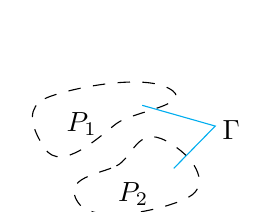
\begin{tikzpicture}[x=0.75pt,y=0.75pt,yscale=-0.4,xscale=0.4]
        %uncomment if require: \path (0,300); %set diagram left start at 0, and has height of 300
        
        %Shape: Polygon Curved [id:ds3275739299185525] 
        \draw  [dash pattern={on 4.5pt off 4.5pt}] (113,73.24) .. controls (133,63.24) and (227.26,41.75) .. (262.26,60.75) .. controls (297.26,79.75) and (219.26,88.26) .. (199.26,103.26) .. controls (179.26,118.26) and (133,163.24) .. (113,133.24) .. controls (93,103.24) and (93,83.24) .. (113,73.24) -- cycle ;
        %Shape: Polygon Curved [id:ds29563927191425465] 
        \draw  [dash pattern={on 4.5pt off 4.5pt}] (199.26,154.26) .. controls (219.26,144.26) and (224.26,105.26) .. (259.26,124.26) .. controls (294.26,143.26) and (310.26,174.26) .. (290.26,189.26) .. controls (270.26,204.26) and (173,228.24) .. (153,198.24) .. controls (133,168.24) and (179.26,164.26) .. (199.26,154.26) -- cycle ;
        %Straight Lines [id:da6767121224748709] 
        \draw [color=cyan  ,draw opacity=1 ]   (268.26,157.26) -- (318.26,106.26) -- (230.26,81.26) ;
        
        % Text Node
        \draw (136,86.4) node [anchor=north west][inner sep=0.75pt]    {$P_{1}$};
        % Text Node
        \draw (198,171.4) node [anchor=north west][inner sep=0.75pt]    {$P_{2}$};
        % Text Node
        \draw (324,96.4) node [anchor=north west][inner sep=0.75pt]    {$\Gamma $};
        
        
        \end{tikzpicture}
        \]In this $\Gamma$ (NOT a region), the clopen subsets are $P_1,P_2,\emptyset,\Gamma$.}
    In a connected region $\reg$, only $\emptyset, \reg$ are clopen.

    Let $S=\{z\in \reg : f^{(j)}(z)=0 \quad \forall\, j=0,1,2,\dots\}$. If $z_0\in S$ then $f$ is zero on some open disk centered at $z_0$. \dashuline{Hence, $S$ is open!}

    Now suppose $w$ is a limit of a sequence in $S$. Since $f$ is continuous, $f^{(j)}$ is continuous for all $j\in \N$. This enruses that $f^{(j)}(w)=0$. \dashuline{Thus, $S$ is closed!}

    Therefore, $S$ is clopen in $\reg$, so either $S$ is the empty set or $S=\reg$. If $S=\reg$, then $f$ is the zero function, so that cannot happen! Therefore, $S=\emptyset$, and so we don't have a cluster of zeros.
\end{proof}

\corollary If $f$ is a nonconstant analytic function, its zero set is \textbf{countable}. This is because within an open region, we can have at most countably infinite number of disjoint open sets. We let these open sets be $f^{-1}(\{0\})$.

\subsection{Identity theorem}
\defn An \textbf{accumulation} point of $S$ is a point that is the limit of a sequence of \textbf{distinct} points of $S$.
\[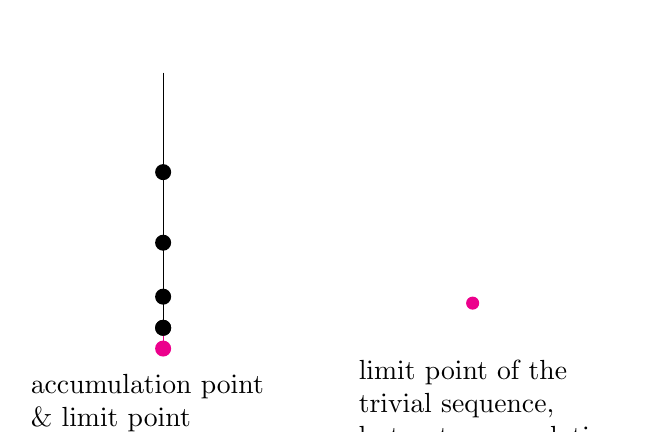
\begin{tikzpicture}[x=0.75pt,y=0.75pt,yscale=-1,xscale=1]
    %uncomment if require: \path (0,300); %set diagram left start at 0, and has height of 300
    
    %Straight Lines [id:da556992577885977] 
    \draw    (100,105.76) -- (100,139.76) ;
    \draw [shift={(100,139.76)}, rotate = 90] [color=black  ][fill=black  ][line width=0.75]      (0, 0) circle [x radius= 3.35, y radius= 3.35]   ;
    %Straight Lines [id:da08524159729103475] 
    \draw    (100,57.76) -- (100,105.76) ;
    \draw [shift={(100,105.76)}, rotate = 90] [color=black  ][fill=black  ][line width=0.75]      (0, 0) circle [x radius= 3.35, y radius= 3.35]   ;
    %Straight Lines [id:da41449224969428156] 
    \draw    (100,139.76) -- (100,165.76) ;
    \draw [shift={(100,165.76)}, rotate = 90] [color=black  ][fill=black  ][line width=0.75]      (0, 0) circle [x radius= 3.35, y radius= 3.35]   ;
    %Straight Lines [id:da4533906108237473] 
    \draw    (100,165.76) -- (100,180.76) ;
    \draw [shift={(100,180.76)}, rotate = 90] [color=black  ][fill=black  ][line width=0.75]      (0, 0) circle [x radius= 3.35, y radius= 3.35]   ;
    %Straight Lines [id:da15251507183156088] 
    \draw [color=magenta  ,draw opacity=1 ]   (100,180.76) -- (100,190.76) ;
    \draw [shift={(100,190.76)}, rotate = 90] [color=magenta  ,draw opacity=1 ][fill=magenta  ,fill opacity=1 ][line width=0.75]      (0, 0) circle [x radius= 3.35, y radius= 3.35]   ;
    %Straight Lines [id:da447461872834491] 
    \draw    (100,165.76) -- (100,180.76) ;
    \draw [shift={(100,180.76)}, rotate = 90] [color=black  ][fill=black  ][line width=0.75]      (0, 0) circle [x radius= 3.35, y radius= 3.35]   ;
    %Shape: Circle [id:dp7661245715545606] 
    \draw  [color=magenta  ,draw opacity=1 ][fill=magenta  ,fill opacity=1 ] (252,168.87) .. controls (252,167.29) and (250.71,166) .. (249.13,166) .. controls (247.54,166) and (246.26,167.29) .. (246.26,168.87) .. controls (246.26,170.46) and (247.54,171.74) .. (249.13,171.74) .. controls (250.71,171.74) and (252,170.46) .. (252,168.87) -- cycle ;
    
    % Text Node
    \draw (35,202) node [anchor=north west][inner sep=0.75pt]   [align=left] {accumulation point \\\& limit point};
    % Text Node
    \draw (193,195) node [anchor=north west][inner sep=0.75pt]   [align=left] {limit point of the \\trivial sequence, \\but not accumulation};
    
    
    \end{tikzpicture}
    \]

\begin{theorem}
    Let $f,g:\reg\to \C$ be analytic. If $f=g$ on a subset of $\reg$ that has an accumulation point in $\reg$, then $f=g$ on the entire $\reg$.
\end{theorem}
\begin{proof}
    If the zero set of $f-g$ has an accumulation point in $\reg$, then $f-g$ has a zero that is not isolated (no open disk around it since some zeros keep converging to that accumulation point), so $f-g$ is identically zero on $\reg$.
\end{proof}

\eg There is only one way to extend $\cos x, \sin x, \exp x$ from $\R$ to $\C$ because two entire functions that agree on $\R$ agree on $\C$. 

\eg Similarly, there is also only one way to get an analytic continuation of the Riemann zeta function to $\re s>0$. 

\subsection{Maximum modulus principle}
Recall this handwavy physics application \hyperlink{physics}{here}. We now have a more rigorous way to state this!\sidenote{Not exactly equivalent, though.}

\begin{theorem}[Maximum modulus principle]
    Let $f$ be analytic on a region $\reg$ that contains a piecewise $C'$ simple closed curve $\gamma$ and its interior. Then \[|f(z)|\leq \max_{\zeta\in \gamma}|f(\zeta)|\] for all $z$ in the interior of $\gamma$.
\end{theorem}
\begin{proof}
    Let $M= \max_{\zeta\in \gamma}|f(\zeta)|$. Fix $z$ inside $\gamma$. Let $L$ denote the length of $\gamma$ and let $r=\inf_{\zeta\in \gamma}|z-\zeta$, which is positive (so $z$ isn't arbitrarily close to $\gamma$). 

    Apply Cauchy's integral formula to the $n$-th power of $f$: \[f(z)^n = \frac{1}{2\pi i}\int_{\gamma}\frac{f(\zeta)^n\d\zeta}{\zeta-z}\]
    Thus, \[|f(z)|^n \leq \frac{1}{2\pi}\cdot \frac{M^n}{r}L\]
    Now we just take the $n$-th root everywhere:\[|f(z)|\leq M\left(\frac{L}{2\pi r}\right)^{1/n}\] We use arbitrarily large $n$ and get $|f(z)|\leq M$.
\end{proof}

\subsection{Schwarz' lemma}
\begin{lemma}[Schwarz']
    Let $f:\D\to \D^-$ be analytic and $f(0)=0$. Then: \begin{enumerate}[label=(\alph*)]
        \item \(|f'(0)|\leq 1\) and $|f(z)|\leq |z|$ for all $z\in \D$.
        \item If $|f'(0)|=1$ or $|f(z_0)|=|z_0|$ for some $z_0\neq 0$, then $f(z)=\lambda z$ for some $\lambda$ with $|\lambda|=1$.
    \end{enumerate}
\end{lemma}

\begin{proof}[Proof part (a)]
    Since $f(0)=0$, we have that the constant term of $f$ is 0, and so $f(z)=zg(z)$ for some $g$ analytic on $\D$. Thus, \[f'(z)=g(z)+zg'(z)\] and hence $f'(0)=g(0)$. Hence, \[g(z)=\begin{cases}
        \frac{f(z)}{z} & z\neq 0\\
        f'(0) &z=0
    \end{cases}\]
    If $|z|\leq r<1$, then by the maximum modulus principle, \begin{align*}
        |g(z)|&\leq \max_{|\zeta|=r}|g(\zeta)|\\
        &= \max_{|\zeta|=r}\left|\frac{f(\zeta)}{\zeta}\right|\\
        &\leq \frac{1}{r} &\text{since }f:\D\to\D^-
    \end{align*}
    Let $r\to 1^-$ and get $|g(z)|\leq 1$ for all $z\in \D$, which is the (a) part of our result.
\end{proof}

\begin{proof}[Proof part (b)]
    Maximum modulus principle says the given conditions imply $g$ is constant. The constant $\lambda$ has absolute value 1, so $\frac{f(z)}{z}=\lambda$ and so $f(z)=\lambda z$.
\end{proof}

\subsection{Automorphism group of a region}
\defn Let $\reg$ be a region in $\C$. We let the automorphism group of the region \(\Aut (\Omega)\) be the set of all \textbf{bijective analytic functions} from $\reg$ to $\reg$.
\begin{itemize}
    \item \(\Aut (\Omega)\) contains the identity function $f(z)=z$.
    \item \(\Aut (\Omega)\) is closed under composition.\sidenote{And composition is a binary operation with associativity}
    \item \(\Aut (\Omega)\) is closed under inverses: if $f:\reg\to\reg$ is an analytic bijection, then $\inv{f}:\reg\to \reg$ exists and is \textbf{analytic}.
    \rmk There appears to be a `counterexample': \[\begin{tikzpicture}[x=0.75pt,y=0.75pt,yscale=-1,xscale=1]
        %uncomment if require: \path (0,300); %set diagram left start at 0, and has height of 300
        
        %Shape: Polynomial [id:dp016145053242946572] 
        \draw   (45,211) .. controls (92.42,73.82) and (139.84,213.69) .. (187.26,76.51) ;
        %Shape: Axis 2D [id:dp40514861748695963] 
        \draw  (37,143.51) -- (204.26,143.51)(119.26,54) -- (119.26,224.51) (197.26,138.51) -- (204.26,143.51) -- (197.26,148.51) (114.26,61) -- (119.26,54) -- (124.26,61)  ;
        %Shape: Axis 2D [id:dp23339690918753542] 
        \draw  (278,143.51) -- (445.26,143.51)(360.26,54) -- (360.26,224.51) (438.26,138.51) -- (445.26,143.51) -- (438.26,148.51) (355.26,61) -- (360.26,54) -- (365.26,61)  ;
        %Shape: Polynomial [id:dp9729500065216796] 
        \draw   (425.26,74.5) .. controls (292.77,120.29) and (427.85,166.09) .. (295.37,211.88) ;
        %Straight Lines [id:da8672984437837188] 
        \draw [color=magenta  ,draw opacity=1 ]   (360.26,143.51) -- (398.91,186.03) ;
        \draw [shift={(400.26,187.51)}, rotate = 227.73] [color=magenta  ,draw opacity=1 ][line width=0.75]    (10.93,-3.29) .. controls (6.95,-1.4) and (3.31,-0.3) .. (0,0) .. controls (3.31,0.3) and (6.95,1.4) .. (10.93,3.29)   ;
        \draw [shift={(360.26,143.51)}, rotate = 47.73] [color=magenta  ,draw opacity=1 ][fill=magenta  ,fill opacity=1 ][line width=0.75]      (0, 0) circle [x radius= 3.35, y radius= 3.35]   ;
        
        % Text Node
        \draw (162,55.4) node [anchor=north west][inner sep=0.75pt]    {$x^{3}$};
        % Text Node
        \draw (433,46.4) node [anchor=north west][inner sep=0.75pt]    {$x^{1/3}$};
        % Text Node
        \draw (376,194) node [anchor=north west][inner sep=0.75pt]  [color=magenta  ,opacity=1 ] [align=left] {not differentiable?};
        
        
        \end{tikzpicture}
        \]
        However, this is only true in $\R$. In $\C$, we observe that $z^3$ is \textbf{not} a bijection at $0$, so this function is not in the group at all!
\end{itemize}

\addlink{Riemann Mapping Theorem}
\begin{theorem}[Riemann Mapping]
    If $\reg$ is simply connected (no holes)\sidenote{Except for the entire $\C$, which has only constant functions if bounded (by Liouville thm).}, then it could be conformally mapped to a disk.
    \drawing{0.5\linewidth}{image-7.png}
\end{theorem}

\spl

Recall from HW1 that for each $w\in \D$, we have a bijection \[\phi_w(z)=\frac{-z+w}{-\bar w z+1}\] from $\D$ to $\D$ and $\phi\circ \phi=\mathrm{id}$. To see this, observe the matrix representation \[\begin{bmatrix}
    -1 & w\\ -\bar w & 1
\end{bmatrix}\cdot \begin{bmatrix}
    -1 & w\\ -\bar w & 1
\end{bmatrix} = \begin{bmatrix}
    1-|w|^2 & 0 \\ 0 &  1-|w|^2
\end{bmatrix}\sim I\]
Furthermore, note $\phi_w(0)=w$. Suppose $f\in \Aut(\D)$, then there is a unique $w\in \D$ such that $f(w)=0$. Define $g=f\circ \phi_w\in \Aut(\D)$. Note that $g(0)=f(\phi_w(0))=f(w)=0$. By Schwarz' lemma, we have \rt{$|g(z)|\leq |z|$} for all $z\in \D$. 

Since $\inv g\in \Aut(\D)$, we also have $|\inv g(z)|\leq |z|$ for all $z\in \D$. Now substitute $g(z)$ for $z$ since it's also in the disk. Hence, \bt{$|z|=|\inv g (g(z))|\leq |g(z)|$}. Therefore, we are forced to conclude that $\textcolor{violet}{|z|=|g(z)|}$ for ALL $z\in \D$!

Since $\textcolor{violet}{|z|=|g(z)|}$ for ALL $z\in \D$, Schwarz' lemma says $g(z)=\lambda z$ for some $|\lambda|=1$. Let $\lambda=e^{i\theta}$ for some $\theta\in \R$. Thus, \[g(z)=f(\phi_w(z))=e^{i\theta}z\]
and so \[e^{i\theta}\phi_w(z)=f(\phi_w(\phi_w(z)))=f(z)\]
since $\phi_w\circ \phi_w=\mathrm{id}$. Therefore, $\displaystyle f(z)=e^{i\theta}\frac{w-z}{1-\bar wz}$.

Therefore, 
\begin{proposition}
    \[\Aut (\D)= \left\{e^{i\theta}\frac{w-z}{1-\bar wz}\; \Bigg \vert\; \theta\in [0,2\pi), w\in \D\right\}\]
\end{proposition}

\rmk The topological representation of the automorphism group of $\D$ is a `skinless torus' (collection of open disks revolving from 0 to $2\pi$).

\subsection{Morera's theorem}
\begin{theorem}[Morera]
    If $f:\reg\to\C$ is continuous and $\int_{\gamma}f(\zeta)\d\zeta=0$ for all \underline{\hspace{2cm}} $\gamma$ in $\reg$, then $f$ is analytic on $\reg$. \sidenote{the blank can be `rectangles', `triangles', `piecewise $C^1$ closed curves', etc.}
\end{theorem}
\begin{proof}[Proof see \href{https://stephangarcia.sites.pomona.edu/teaching/24S-135/Lecture/24S-135-Lecture16.pdf}{notes}]
\end{proof}

\subsection{Weierstrass convergence theorem}
Let $f_n(z)$ be analytic for every $n\in \N$. We are still not sure that $\sum_{n=1}^{\infty} f_n(z)$ is analytic yet!

\begin{theorem}[Weierstrass convergence]
    If $f_n:\reg\to \C$ are analytic and $f_n$ converges \textit{locally uniformly} on $\reg$ to the limit function $f$ (\bt{$\Leftrightarrow$ uniform convergence on compact sets}), then \textcolor{darkgray}{$f$ is analytic and for each fixed $m$, $f_n^{m}$ converges to $f^{(m)}$ locally uniformly on $\reg$ and $f$ is infinitely differentiable}. 
\end{theorem}

\rmk This is a huge contrast with the\textit{ Weierstrass approximation theorem} in real analysis, which says that \textcolor{darkgray}{if $f:[0,1]\to \R$, then there is a sequence of polynomials $p_n$ such that $p_n$ converges to $f$ uniformly on $[0,1]$}. That is, even the most pathological, nowhere-differentiable functions in $\R$ are a limit of some polynomial sequences! However, in the $\C$ world, the limit of any analytic function is still analytic.

\section{Laurent series \& isolated singularities}
Sometimes the domain $\reg$ isn't the largest domain where an analytic function can be analytic. So far, we know we can find the largest disk centered at a point in $\reg$\sidenote{the disk could exceed the bounds of $\reg$!} in which a function is analytic and the power series exists there:\[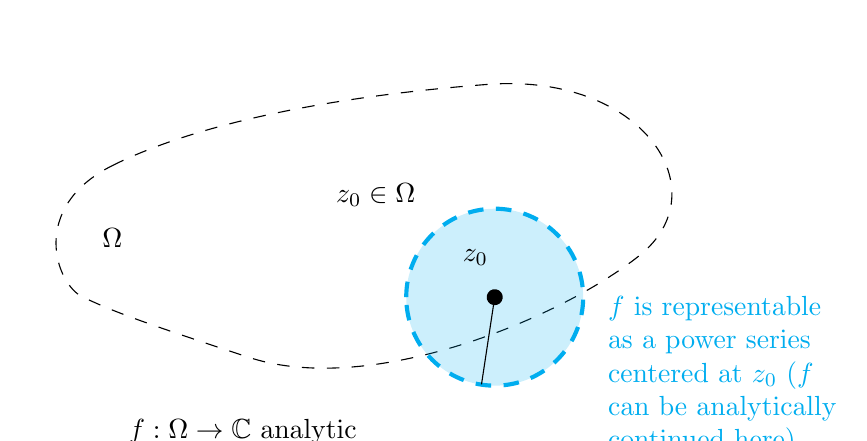
\begin{tikzpicture}[x=0.75pt,y=0.75pt,yscale=-1,xscale=1]
    %uncomment if require: \path (0,300); %set diagram left start at 0, and has height of 300
    
    %Shape: Polygon Curved [id:ds40363339954426203] 
    \draw  [dash pattern={on 4.5pt off 4.5pt}] (105.36,58.25) .. controls (145.83,38.01) and (210.86,24.86) .. (286.14,19.12) .. controls (361.42,13.38) and (398.26,70.64) .. (359.26,101.64) .. controls (320.26,132.64) and (229.26,169.64) .. (171.26,150.64) .. controls (113.26,131.64) and (104.26,127.64) .. (91.26,121.64) .. controls (78.26,115.64) and (64.88,78.49) .. (105.36,58.25) -- cycle ;
    %Shape: Circle [id:dp18109739983497897] 
    \draw  [color=cyan  ,draw opacity=1 ][fill=cyan  ,fill opacity=0.2 ][dash pattern={on 5.63pt off 4.5pt}][line width=1.5]  (247,121.63) .. controls (247,98.09) and (266.09,79) .. (289.63,79) .. controls (313.17,79) and (332.26,98.09) .. (332.26,121.63) .. controls (332.26,145.17) and (313.17,164.26) .. (289.63,164.26) .. controls (266.09,164.26) and (247,145.17) .. (247,121.63) -- cycle ;
    %Straight Lines [id:da39916826624746937] 
    \draw    (289.63,121.63) -- (283.26,163.64) ;
    \draw [shift={(289.63,121.63)}, rotate = 98.62] [color=black  ][fill=black  ][line width=0.75]      (0, 0) circle [x radius= 3.35, y radius= 3.35]   ;
    
    % Text Node
    \draw (99.38,87.08) node [anchor=north west][inner sep=0.75pt]    {$\Omega $};
    % Text Node
    \draw (273,97.4) node [anchor=north west][inner sep=0.75pt]    {$z_{0}$};
    % Text Node
    \draw (343,120) node [anchor=north west][inner sep=0.75pt]  [color=cyan  ,opacity=1 ] [align=left] {$\displaystyle f$ is representable\\as a power series \\centered at $\displaystyle z_{0}$ ($\displaystyle f$ \\can be analytically\\continued here)};
    % Text Node
    \draw (212,65.4) node [anchor=north west][inner sep=0.75pt]    {$z_{0} \in \Omega $};
    % Text Node
    \draw (112,179) node [anchor=north west][inner sep=0.75pt]   [align=left] {$\displaystyle f:\Omega \rightarrow \mathbb{C}$ analytic};
    
    
    \end{tikzpicture}\]

Can we do even better than that?

\subsection{Laurent series}
\eg Let $f(z)=\frac{1}{z(z-1)}$ analytic on $\C\backslash\{0,1\}$. We realize that if we restrict $0<|z|<1$, then \[f(z)=\frac{-1}{z}\cdot\frac{1}{1-z}=\frac{-1}{z}-1-z-z^2-\dots\] 
is the \textbf{Laurent series} of $f(z)$ centered at 0, a point where $f(z)$ isn't even defined!

\eg We continue with the previous function. This time, we restrict $|z|>1$ and express it as:\[f(z)=\frac{1}{z^2(1-\frac{1}{z})} = \frac{1}{z^2}+\frac{1}{z^3}+\dots\]

Hence, we now have different series for $f$ in different regions: \[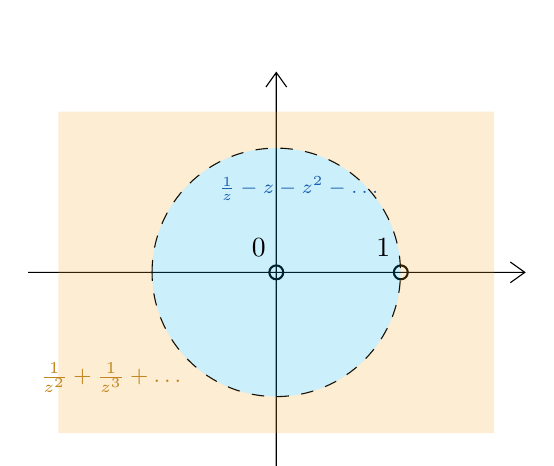
\begin{tikzpicture}[x=0.75pt,y=0.75pt,yscale=-1,xscale=1]
    %uncomment if require: \path (0,300); %set diagram left start at 0, and has height of 300
    
    %Shape: Axis 2D [id:dp8096713031018239] 
    \draw  (60.49,170) -- (299.74,170)(180,73.71) -- (180,270.86) (292.74,165) -- (299.74,170) -- (292.74,175) (175,80.71) -- (180,73.71) -- (185,80.71)  ;
    %Straight Lines [id:da8307990020001665] 
    \draw    (182.35,170) -- (237.65,170) ;
    \draw [shift={(240,170)}, rotate = 0] [color=black  ][line width=0.75]      (0, 0) circle [x radius= 3.35, y radius= 3.35]   ;
    \draw [shift={(180,170)}, rotate = 0] [color=black  ][line width=0.75]      (0, 0) circle [x radius= 3.35, y radius= 3.35]   ;
    %Shape: Circle [id:dp6485221177915352] 
    \draw  [fill=cyan  ,fill opacity=0.2 ][dash pattern={on 4.5pt off 4.5pt}] (120.14,170) .. controls (120.14,136.94) and (146.94,110.14) .. (180,110.14) .. controls (213.06,110.14) and (239.86,136.94) .. (239.86,170) .. controls (239.86,203.06) and (213.06,229.86) .. (180,229.86) .. controls (146.94,229.86) and (120.14,203.06) .. (120.14,170) -- cycle ;
    %Shape: Path Data [id:dp866707860246108] 
    \draw  [draw opacity=0][fill={rgb, 255:red, 245; green, 166; blue, 35 }  ,fill opacity=0.2 ][dash pattern={on 4.5pt off 4.5pt}] (180,110.14) .. controls (213.06,110.14) and (239.86,136.94) .. (239.86,170) .. controls (239.86,203.06) and (213.06,229.86) .. (180,229.86) .. controls (146.94,229.86) and (120.14,203.06) .. (120.14,170) .. controls (120.14,136.94) and (146.94,110.14) .. (180,110.14) -- cycle (75,92.5) -- (75,247.5) -- (285,247.5) -- (285,92.5) -- (75,92.5) -- cycle ;
    
    % Text Node
    \draw (167,152.4) node [anchor=north west][inner sep=0.75pt]    {$0$};
    % Text Node
    \draw (227,152.4) node [anchor=north west][inner sep=0.75pt]    {$1$};
    % Text Node
    \draw (151,122.4) node [anchor=north west][inner sep=0.75pt]  [font=\scriptsize,color={rgb, 255:red, 25; green, 96; blue, 175 }  ,opacity=1 ]  {$\frac{1}{z} -z-z^{2} -\dotsc $};
    % Text Node
    \draw (65,212.4) node [anchor=north west][inner sep=0.75pt]  [font=\footnotesize,color={rgb, 255:red, 194; green, 132; blue, 28 }  ,opacity=1 ]  {$\frac{1}{z^{2}} +\frac{1}{z^{3}} +\dotsc $};
    
    
    \end{tikzpicture}
    \]

\defn[Laurent series] A series in the form $\displaystyle \sum_{\rt{n=-\infty}}^{\infty}a_n(z-z_0)^n$ is a \textbf{Laurent series}. It converges at $z\in \C$ if \textbf{both} the \uline{analytic part} \(\displaystyle \sum_{\rt{n=0}}^{\infty}a_n(z-z_0)^n\) and the \uline{principal part} \(\displaystyle \sum_{n=1}^{\infty}a_{\bt{-n}}(z-z_0)^{\bt{-n}}\) converge at $z$. If this occurs, the Laurent series would be \[\sum_{\rt{n=-\infty}}^{\infty}a_n(z-z_0)^n = \sum_{\rt{n=0}}^{\infty}a_n(z-z_0)^n +\sum_{n=1}^{\infty}a_{\bt{-n}}(z-z_0)^{\bt{-n}}\] and also converges.

\lemma Recall that if $n\neq -1$, then $\frac{(z-z_0)^{n+1}}{n+1}$ is an antiderivative of $(z-z_0)^n$ on $\C$. \textbf{So} if $\gamma$ is simple closed, then by FTC, \[\frac{1}{2\pi i}\int_{\gamma}(z-z_0)^n\d z=0\] whenever $n\neq 1$. In addition, by Cauchy's integral formula, $\frac{1}{2\pi i}\int_{\gamma}\frac{\d z}{z-z_0}=1$. Therefore, if $z_0$ is in the interior of a simple closed curve $\gamma$, then \[\frac{1}{2\pi i}\int_{\gamma}(z-z_0)^n\d z= \begin{cases}
    0 & n\neq -1\\
    1 & n=-1
\end{cases}\]

\begin{proof}
    We previously know the result above when $\gamma$ is a circle. We now extend it to all simple closed curves by a familiar trick as follows:
    \[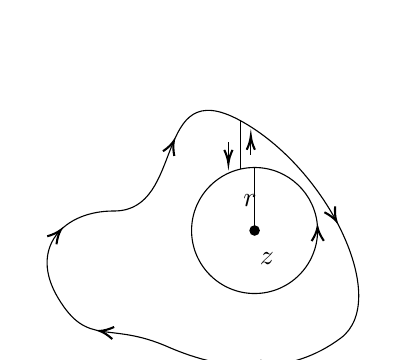
\begin{tikzpicture}[x=0.75pt,y=0.75pt,yscale=-.6,xscale=.6]
        %uncomment if require: \path (0,300); %set diagram left start at 0, and has height of 300
        
        %Curve Lines [id:da7016804119762063] 
        \draw    (150.26,97.76) .. controls (208.26,97.76) and (180.42,-13.45) .. (251.26,25) .. controls (322.09,63.45) and (372.73,169.41) .. (332.26,199.76) .. controls (291.78,230.12) and (241.26,227.76) .. (193.26,206.76) .. controls (145.26,185.76) and (129.26,207.64) .. (105.26,167.64) .. controls (81.26,127.64) and (109.26,97.51) .. (150.26,97.76) -- cycle ;
        \draw [shift={(198.18,41.55)}, rotate = 112.47] [color=black  ][line width=0.75]    (10.93,-4.9) .. controls (6.95,-2.3) and (3.31,-0.67) .. (0,0) .. controls (3.31,0.67) and (6.95,2.3) .. (10.93,4.9)   ;
        \draw [shift={(328.72,105.93)}, rotate = 240.89] [color=black  ][line width=0.75]    (10.93,-4.9) .. controls (6.95,-2.3) and (3.31,-0.67) .. (0,0) .. controls (3.31,0.67) and (6.95,2.3) .. (10.93,4.9)   ;
        \draw [shift={(257.73,222.48)}, rotate = 0.74] [color=black  ][line width=0.75]    (10.93,-4.9) .. controls (6.95,-2.3) and (3.31,-0.67) .. (0,0) .. controls (3.31,0.67) and (6.95,2.3) .. (10.93,4.9)   ;
        \draw [shift={(138.71,194.06)}, rotate = 8.82] [color=black  ][line width=0.75]    (10.93,-4.9) .. controls (6.95,-2.3) and (3.31,-0.67) .. (0,0) .. controls (3.31,0.67) and (6.95,2.3) .. (10.93,4.9)   ;
        \draw [shift={(107.34,112.99)}, rotate = 130.63] [color=black  ][line width=0.75]    (10.93,-4.9) .. controls (6.95,-2.3) and (3.31,-0.67) .. (0,0) .. controls (3.31,0.67) and (6.95,2.3) .. (10.93,4.9)   ;
        %Shape: Arc [id:dp13815379083723078] 
        \draw  [draw opacity=0] (313.61,113.43) .. controls (313.61,113.43) and (313.61,113.43) .. (313.61,113.43) .. controls (313.61,141.37) and (290.96,164.02) .. (263.02,164.02) .. controls (235.07,164.02) and (212.42,141.37) .. (212.42,113.43) .. controls (212.42,85.48) and (235.07,62.83) .. (263.02,62.83) .. controls (290.66,62.83) and (313.13,85.01) .. (313.6,112.54) -- (263.02,113.43) -- cycle ; \draw    (313.61,113.43) .. controls (313.61,113.43) and (313.61,113.43) .. (313.61,113.43) .. controls (313.61,141.37) and (290.96,164.02) .. (263.02,164.02) .. controls (235.07,164.02) and (212.42,141.37) .. (212.42,113.43) .. controls (212.42,85.48) and (235.07,62.83) .. (263.02,62.83) .. controls (290.11,62.83) and (312.23,84.13) .. (313.55,110.9) ; \draw [shift={(313.55,110.9)}, rotate = 89.02] [color=black  ][line width=0.75]    (10.93,-4.9) .. controls (6.95,-2.3) and (3.31,-0.67) .. (0,0) .. controls (3.31,0.67) and (6.95,2.3) .. (10.93,4.9)   ; 
        %Straight Lines [id:da8914465255998514] 
        \draw    (263.02,62.83) -- (263.02,113.43) ;
        \draw [shift={(263.02,113.43)}, rotate = 90] [color=black  ][fill=black  ][line width=0.75]      (0, 0) circle [x radius= 3.35, y radius= 3.35]   ;
        %Straight Lines [id:da9471588673663345] 
        \draw    (252,25) -- (252,64.26) ;
        %Straight Lines [id:da9805830469698456] 
        \draw    (242,42.64) -- (242,57.64) ;
        \draw [shift={(242,59.64)}, rotate = 270] [color=black  ][line width=0.75]    (10.93,-3.29) .. controls (6.95,-1.4) and (3.31,-0.3) .. (0,0) .. controls (3.31,0.3) and (6.95,1.4) .. (10.93,3.29)   ;
        %Straight Lines [id:da036041464758245434] 
        \draw    (260,52.64) -- (260,39.64) ;
        \draw [shift={(260,37.64)}, rotate = 90] [color=black  ][line width=0.75]    (10.93,-3.29) .. controls (6.95,-1.4) and (3.31,-0.3) .. (0,0) .. controls (3.31,0.3) and (6.95,1.4) .. (10.93,3.29)   ;
        
        % Text Node
        \draw (265.21,129.09) node [anchor=north west][inner sep=0.75pt]    {$z$};
        % Text Node
        \draw (251.95,82.47) node [anchor=north west][inner sep=0.75pt]    {$r$};
        
        
        \end{tikzpicture}
        \]
\end{proof}

\subsubsection{Laurent expansion theorem}
\theorem[Laurent expansion] Suppose $f$ is analytic on the annular region $A=\{z\in \C\mid R_1<|z-z_0|<R_2\}$.\sidenote{$R_1=0,R_2=\infty$ are okay} Then $f$ has a locally uniformly convergent Laurent expansion $$
f(z)=\sum_{n=-\infty}^{\infty} a_n\left(z-z_0\right)^n
$$
on $A$. Moreover, the Laurent coefficients are
$$
a_n=\frac{1}{2 \pi i} \int_{C_r\left(z_0\right)} \frac{f(\zeta) d \zeta}{\left(\zeta-z_0\right)^{n+1}}
$$
for any $r$ such that $R_1<r<R_2$.

\begin{proof}[Proof gist]
    For a gist of why this works:\sidenote{For rigorous proof, see \href{https://stephangarcia.sites.pomona.edu/teaching/24S-135/Lecture/24S-135-Lecture17.pdf}{notes}.} \[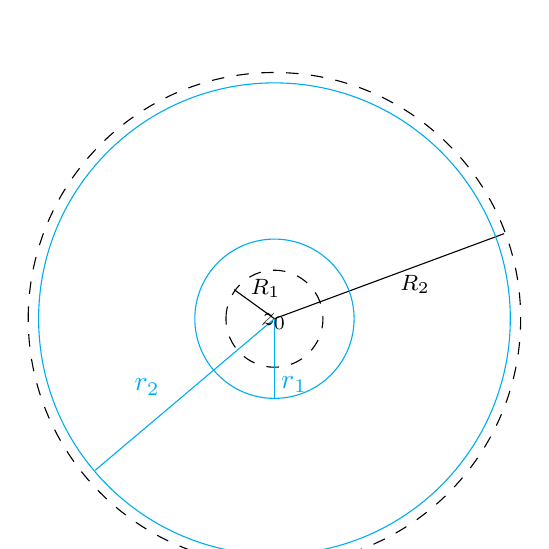
\begin{tikzpicture}[x=0.75pt,y=0.75pt,yscale=-1,xscale=1]
        %uncomment if require: \path (0,300); %set diagram left start at 0, and has height of 300
        
        %Shape: Donut [id:dp6671669505060469] 
        \draw  [dash pattern={on 4.5pt off 4.5pt}] (160.26,142.63) .. controls (160.26,129.72) and (170.72,119.26) .. (183.63,119.26) .. controls (196.54,119.26) and (207,129.72) .. (207,142.63) .. controls (207,155.54) and (196.54,166) .. (183.63,166) .. controls (170.72,166) and (160.26,155.54) .. (160.26,142.63)(65,142.63) .. controls (65,77.11) and (118.11,24) .. (183.63,24) .. controls (249.14,24) and (302.26,77.11) .. (302.26,142.63) .. controls (302.26,208.14) and (249.14,261.26) .. (183.63,261.26) .. controls (118.11,261.26) and (65,208.14) .. (65,142.63) ;
        %Straight Lines [id:da7057757873892656] 
        \draw    (164.26,128.64) -- (183.63,142.63) ;
        %Straight Lines [id:da14630762957011] 
        \draw    (183.63,142.63) -- (294.26,101.64) ;
        %Shape: Donut [id:dp20910873444708722] 
        \draw  [color=cyan  ,draw opacity=1 ] (145.26,142.63) .. controls (145.26,121.44) and (162.44,104.26) .. (183.63,104.26) .. controls (204.82,104.26) and (222,121.44) .. (222,142.63) .. controls (222,163.82) and (204.82,181) .. (183.63,181) .. controls (162.44,181) and (145.26,163.82) .. (145.26,142.63)(70,142.63) .. controls (70,79.87) and (120.87,29) .. (183.63,29) .. controls (246.38,29) and (297.26,79.87) .. (297.26,142.63) .. controls (297.26,205.38) and (246.38,256.26) .. (183.63,256.26) .. controls (120.87,256.26) and (70,205.38) .. (70,142.63) ;
        %Straight Lines [id:da5929669596751745] 
        \draw [color=cyan  ,draw opacity=1 ]   (183.63,142.63) -- (97.26,215.64) ;
        %Straight Lines [id:da5310962334011069] 
        \draw [color=cyan  ,draw opacity=1 ]   (183.63,142.63) -- (183.63,181) ;
        
        % Text Node
        \draw (175.94,139.04) node [anchor=north west][inner sep=0.75pt]    {$z_{0}$};
        % Text Node
        \draw (171,122.4) node [anchor=north west][inner sep=0.75pt]  [font=\footnotesize]  {$R_{1}$};
        % Text Node
        \draw (243,120.4) node [anchor=north west][inner sep=0.75pt]  [font=\footnotesize]  {$R_{2}$};
        % Text Node
        \draw (115,170.4) node [anchor=north west][inner sep=0.75pt]    {$\textcolor{cyan}{r_{2}}$};
        % Text Node
        \draw (185.63,169.4) node [anchor=north west][inner sep=0.75pt]    {$\textcolor{cyan}{r}\textcolor{cyan}{_{1}}$};
        
        
        \end{tikzpicture}
        \]

        Cauchy's integral formula reveals that
        $$
        f(z)=\frac{1}{2 \pi i} \int_{C_{r_2}\left(z_0\right)} \frac{f(\zeta) \d \zeta}{\zeta-z}-\frac{1}{2 \pi i} \int_{C_{r_1}\left(z_0\right)} \frac{f(\zeta) \d \zeta}{\zeta-z}
        $$
        whenever
        $$
        R_1<r_1<|z|<r_2<R_2 .
        $$
        
        These integrals are independent of $r_1$ and $r_2$ so long as $r_1<|z|<r_2$.
\end{proof}


\rmk If $n\geq 0$ and $f$ is analytic on $|z|<R_2$, then we should get that the Taylor series expansion and the Laurent expansion for the same function $f$ to match. They indeed do match by Cauchy's integral formula:\[a_{n}=\frac{f^{(n)}(z_{0})}{n!}=\frac{1}{2\pi i}\int_{C_{r}(z_{0})}\frac{f(\zeta)\d\zeta}{(\zeta-z_{0})^{n+1}}\]

\subsection{Isolated singularities}
\defn If $f$ is analytic on $0<|z-z_0|<R$ (a \underline{deleted neighbourhood} of $z_0$), then $z_0$ is an \textbf{isolated singularity} of $f$.

\defn If the principal part of the Laurent expansion for $f$ at $z_0$ is 0 (i.e. $a_{-1}=a_{-2}=\dots=0)$, then $z_0$ is a \textbf{removable singularity} of $f$. The Laurent expansion for $f$ at $z_0$ is simply a power series \(f(z)=\sum_{n=0}^{\infty}a_n(z-z_0)^n\) suggests we set $f(z_0)=a_0$, in which case $f$ is analytic at $z_0$.

\eg Observe \begin{align*}
    \frac{\sin z}{z}&= \frac{1}{z}\left(z-\frac{z^3}{3!}+\frac{z^5}{5!}-\dots\right)\\
    &= \rt{1}-\frac{z^2}{3!}+\frac{z^4}{5!}-\dots
\end{align*}
We define $f(0)=1$, so $\frac{\sin z}{z}$ is actually entire!\sidenote{This agrees with L'H\^opital's rule.}

\addlink{Conditions for removable singularity}
\begin{theorem}
    If $z_0$ is an isolated singularity of an analytic function $f$, then $z_0$ is removable \ifnif any of the following hold:\begin{enumerate}[label=(\alph*)]
        \item $f$ is bounded on some deleted neighbourhood of $z_0$
        \item $\lim_{z\to z_0}f(z)$ exists\sidenote{$\infty$ doesn't count}
        \item $\lim_{z\to z_0}(z-z_0)f(z)=0$
    \end{enumerate}
\end{theorem}
\rmk (a) and (b) implies (c), (b) implies (a).
\begin{proof}It suffices to show that (c) $\iff$ removable.
    \begin{enumerate}
        \item[($\implies$)] If $z_0$ is removable, then $f$ is analytic at $z_0$, so all of the above follow.
        
        \item[($\impliedby$)]  Suppose (c) holds. Then for all $\varepsilon>0$, there exists $0\leq r<1$ such that whenever $|z-z_0|<2r$, we have $|f(z)(z-z_0)|<\varepsilon$.
        
        Then, for all $n\geq 1$, we have \begin{align*}
            |a_{-n}|&=\left|\frac{1}{2\pi i}\int_{C_r(z_0)}f(\zeta)(\zeta-z_0)^{n-1}\d \zeta\right|\\
            &= \left|\frac{1}{2\pi i}\int_{C_r(z_0)}\rt{f(\zeta)(\zeta-z_0)}(\zeta-z_0)^{n-2}\d \zeta\right|\\
            &\leq \frac{1}{2\pi}\cdot \rt{\varepsilon}r^{n-2}2\pi r\\
            &= \varepsilon r^{n-1}\\
            &<\varepsilon
        \end{align*}
        Thus, $a_{-n}=0$ for all $n\geq 1$. The principal part of the Laurent expansion of $f$ is zero.
    \end{enumerate}
\end{proof}

\addlink{Poles}
\defn If the principal part of $f$ at $z_0$ is of the form \[\frac{a_{-n}}{(z-z_0)^{n}}+\frac{a_{-(n-1)}}{(z-z_0)^{n-1}}+\dots +\frac{a_{-1}}{(z-z_0)}\] where $a_{-n}\neq 0$, then $z_0$ is a \textbf{pole} of $f$ of order $n$.\sidenote{$n$ must be \textbf{finite} such that we can clear the denominator}

\defn A pole of order 1 is a \textbf{simple pole}.

\begin{theorem}
    If $z_0$ is an isolated singularity of $f$, then $z_0$ is a \textbf{pole} of order $\leq n$ \ifnif there is an analytic $\phi(z)$ on a \textcolor{gray}{deleted}\sidenote{Return to the full neighbourhood by the trick of removable singularity} neighbourhood of $z_0$ such that \[f(z)=\frac{\phi(z)}{(z-z_0)^n}\]
    This occurs \ifnif any of the following hold: \begin{enumerate}[label=(\alph*)]
        \item $(z-z_0)^nf(z)$ is bounded on some deleted neighbourhood of $z_0$
        \item $\lim_{z\to z_0}f(z)(z-z_0)^n$ exists
        \item $\lim_{z\to z_0}f(z)(z-z_0)^{n+1}=0$
    \end{enumerate}
\end{theorem}

\rmk We can think of poles and zeros in the following fashion: 

\begin{tabular}{ll}
   $f(z)=(z-z_0)^jF(z)$ & $g(z) = \frac{G(z)}{(z-z_0)^k}$\\
   $f$ has a zero of order $j$ at $z_0$ & $g$ has a pole of order $k$ at $z_0$\\
   $F$ doesn't vanish at $z_0$ & $G$ doesn't vanish at $z_0$
\end{tabular}
Then: \[f(z)g(z)=(z-z_0)^{\rt{j-k}}F(z)G(z)\]
\begin{itemize}
    \item If $j=k$, $z_0$ is a removable singularity for $fg$ and is not a zero.
    \item If $j>k$, then $z_0$ is a zero.
    \item If $k>j$, then $z_0$ is a pole.
\end{itemize}

Poles are nice! They could be removed like the denominators of rational functions. However, some other singularities cannot do so.

\defn If the principal part of the Laurent series for $f$ at $z_0$ is $\sum_{n=1}^{\infty}a_{-n}(z-z_0)^{-n}$ where \textbf{infinitely} many $a_{-n}\neq 0$, then $z_0$ is an essential singularity of $f$.

\rmk It is not hard to make an essential singularity: take any entire function with infinite power series. Plug in $\frac{1}{x}$ instead of $x$.

\eg $e^{\frac{1}{x}} = \sum_{n=0}^{\infty}\frac{1}{n!z^n}$ has an essential singularity at $0$.

\begin{theorem}[Casorati-Weierstrass]
    Let $z_0$ be an essential singularity of $f$. For \textbf{each} $w\in \C$\sidenote{This is wild! $f$ could almost splatter everywhere near $z_0$. There isn't a reasonable value to assign to $f(z_0)$.}, there is a sequence $z_n (n\geq 1)$ such that $z_n\to z_0$ and $f(z_n)\to w$.
\end{theorem}
\begin{proof}
    Suppose towards a contradiction that there exists $w\in \C$ such that no such $z_n$ exists. Then there exists $\varepsilon>0$ and $\delta>0$ such that when $0<|z-z_0|<\delta$, we have $|f(z)-w|\geq \varepsilon$ (that is, $f$ is not getting close to $w$). Thus, $g(z)=\frac{1}{f(z)-w}$ is analytic on $0<|z-z_0|<\delta$ and $|g(z)|\leq \frac{1}{\varepsilon}$ there. \dashuline{The singularity $z_0$ of $g$ is therefore removable.} Then $f(z)=w+\frac{1}{g(z)}$, which is either analytic or has a pole at $z_0$ (if $g(z_0)=0$). This causes a contradiction.
\end{proof}

\begin{theorem}[Great Picard]
    If $z_0$ is an essential singularity of $f$, then in any deleted neighbourhood of $z_0$, we have $f$ assuming \textbf{every} complex value \textcolor{gray}{(with at most one exception)} \textbf{infinitely} many times.
\end{theorem}

\eg $f(z)=e^{\frac{1}{z}}$ has an essential singularity at $z_0=0$. (Note $f(z)\neq 0$ is the \textcolor{gray}{exceptional value} that is never assumed.) Let $w\neq 0$ and let $z=\frac{1}{\log w}$ where $\log w$ is a nonzero logarithm of $w$\sidenote{so no 1 for $w$}. Then \[f(z)=e^{\frac{1}{1/\log w}}=e^{\log w}=w\]


\begin{theorem}[Little Picard]
    If $f$ is entire and nonconstant, then $f$ assumes every complex value, \textcolor{gray}{with at most one exception}.
\end{theorem}
\begin{proof}
    If $f$ is a nonconstant polynomial and $w\in \C$, then the polynomial $f(z)-w$ has a zero in $\C$ by the Fundamental Theorem of Algebra, so $f$ assumes the value of $w$.

    If $f$ is not a polynomial\sidenote{Non-polynomial means the Taylor series is infinite}, then $f(\frac{1}{z})$ has an essential singularity at $0$. Then use Great Picard Thm.
\end{proof}

% \section{Residue Theory}
\subsection{Residues}
\defn Let the Laurent series $f(z)=\sum_{n=-\infty}^{\infty} a_n(z-z_0)^n$ be analytic at $0<|z-z_0|<R$. The coefficient $a_{-1}$ is the \textbf{residue} of $f$ at $z_0$. Notation:\[\Res (f;z_0)=a_{-1}\]

\addlink{Residue theorem (simple version)}
\begin{theorem}[Residue, simple vers.] Let $f:\Omega\to \C$ analytic except on the isolated singularity $z_0$. Then:\[\frac{1}{2\pi i}\int_{\gamma}f(\zeta)\,d\zeta=\Res(f\cdotp z_{0}) \]
for any simple closed curve $\gamma$ in $\reg$ with $z_0$ in its interior and whose interior is contained
in $\reg$.
    \[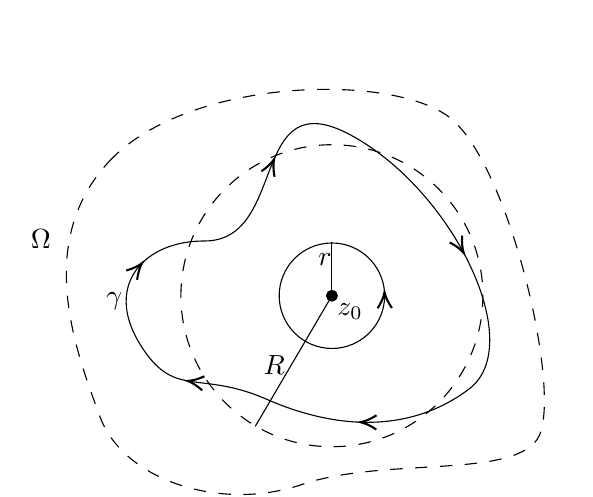
\begin{tikzpicture}[x=0.75pt,y=0.75pt,yscale=-0.7,xscale=.7]
        %uncomment if require: \path (0,300); %set diagram left start at 0, and has height of 300
        
        %Curve Lines [id:da5572659059338843] 
        \draw    (194.26,120.76) .. controls (252.26,120.76) and (224.42,9.55) .. (295.26,48) .. controls (366.09,86.45) and (416.73,192.41) .. (376.26,222.76) .. controls (335.78,253.12) and (285.26,250.76) .. (237.26,229.76) .. controls (189.26,208.76) and (173.26,230.64) .. (149.26,190.64) .. controls (125.26,150.64) and (153.26,120.51) .. (194.26,120.76) -- cycle ;
        \draw [shift={(242.18,64.55)}, rotate = 112.47] [color=black  ][line width=0.75]    (10.93,-4.9) .. controls (6.95,-2.3) and (3.31,-0.67) .. (0,0) .. controls (3.31,0.67) and (6.95,2.3) .. (10.93,4.9)   ;
        \draw [shift={(372.72,128.93)}, rotate = 240.89] [color=black  ][line width=0.75]    (10.93,-4.9) .. controls (6.95,-2.3) and (3.31,-0.67) .. (0,0) .. controls (3.31,0.67) and (6.95,2.3) .. (10.93,4.9)   ;
        \draw [shift={(301.73,245.48)}, rotate = 0.74] [color=black  ][line width=0.75]    (10.93,-4.9) .. controls (6.95,-2.3) and (3.31,-0.67) .. (0,0) .. controls (3.31,0.67) and (6.95,2.3) .. (10.93,4.9)   ;
        \draw [shift={(182.71,217.06)}, rotate = 8.82] [color=black  ][line width=0.75]    (10.93,-4.9) .. controls (6.95,-2.3) and (3.31,-0.67) .. (0,0) .. controls (3.31,0.67) and (6.95,2.3) .. (10.93,4.9)   ;
        \draw [shift={(151.34,135.99)}, rotate = 130.63] [color=black  ][line width=0.75]    (10.93,-4.9) .. controls (6.95,-2.3) and (3.31,-0.67) .. (0,0) .. controls (3.31,0.67) and (6.95,2.3) .. (10.93,4.9)   ;
        %Shape: Arc [id:dp6365443389380805] 
        \draw  [draw opacity=0] (318.31,158.43) .. controls (318.31,158.43) and (318.31,158.43) .. (318.31,158.43) .. controls (318.31,178.47) and (302.06,194.72) .. (282.02,194.72) .. controls (261.97,194.72) and (245.73,178.47) .. (245.73,158.43) .. controls (245.73,138.38) and (261.97,122.13) .. (282.02,122.13) .. controls (301.85,122.13) and (317.96,138.04) .. (318.3,157.79) -- (282.02,158.43) -- cycle ; \draw    (318.31,158.43) .. controls (318.31,158.43) and (318.31,158.43) .. (318.31,158.43) .. controls (318.31,178.47) and (302.06,194.72) .. (282.02,194.72) .. controls (261.97,194.72) and (245.73,178.47) .. (245.73,158.43) .. controls (245.73,138.38) and (261.97,122.13) .. (282.02,122.13) .. controls (301.25,122.13) and (316.99,137.1) .. (318.23,156.03) ; \draw [shift={(318.23,156.03)}, rotate = 89.02] [color=black  ][line width=0.75]    (10.93,-4.9) .. controls (6.95,-2.3) and (3.31,-0.67) .. (0,0) .. controls (3.31,0.67) and (6.95,2.3) .. (10.93,4.9)   ; 
        %Straight Lines [id:da45398740116247227] 
        \draw    (282.02,121.14) -- (282.02,158.43) ;
        \draw [shift={(282.02,158.43)}, rotate = 90] [color=black  ][fill=black  ][line width=0.75]      (0, 0) circle [x radius= 3.35, y radius= 3.35]   ;
        %Shape: Circle [id:dp805037477764748] 
        \draw  [dash pattern={on 4.5pt off 4.5pt}] (178.08,158.43) .. controls (178.08,101.02) and (224.62,54.49) .. (282.02,54.49) .. controls (339.42,54.49) and (385.95,101.02) .. (385.95,158.43) .. controls (385.95,215.83) and (339.42,262.36) .. (282.02,262.36) .. controls (224.62,262.36) and (178.08,215.83) .. (178.08,158.43) -- cycle ;
        %Straight Lines [id:da797182999934565] 
        \draw    (282.02,158.43) -- (229.26,248.39) ;
        %Shape: Polygon Curved [id:ds5262648953621514] 
        \draw  [dash pattern={on 4.5pt off 4.5pt}] (129.26,65.39) .. controls (182.26,9.39) and (318.51,4.79) .. (361.26,34.39) .. controls (404,64) and (442.26,230.39) .. (423.26,257.39) .. controls (404.26,284.39) and (317.26,269.39) .. (261.26,288.39) .. controls (205.26,307.39) and (138.26,285.39) .. (122.26,241.39) .. controls (106.26,197.39) and (76.26,121.39) .. (129.26,65.39) -- cycle ;
        
        % Text Node
        \draw (284.02,161.83) node [anchor=north west][inner sep=0.75pt]    {$z_{0}$};
        % Text Node
        \draw (270.95,127.47) node [anchor=north west][inner sep=0.75pt]    {$r$};
        % Text Node
        \draw (233.26,197.79) node [anchor=north west][inner sep=0.75pt]    {$R$};
        % Text Node
        \draw (125,154.4) node [anchor=north west][inner sep=0.75pt]    {$\gamma $};
        % Text Node
        \draw (73,111.4) node [anchor=north west][inner sep=0.75pt]    {$\Omega $};
        
        
        \end{tikzpicture}
        \]
\end{theorem}
\begin{proof}
    The Laurent expansion $f(z)\,=\,\sum_{n=-\infty}^{\infty}\,a_{n}(z\,-\,z_{0})^{n}$ converges locally uniformly on some punctured disk $0 < |z - z_0| < R$. If $r \in (0, R)$ is sufficiently small, then the deformation version of Cauchy's theorem implies \begin{align*}
        \frac{1}{2\pi i}\int_{\gamma}f(z)\d z&=\frac{1}{2\pi i}\int_{C_{r}(z_{0})}f(z)\d z\\
        &=\frac{1}{2\pi i}\int_{C_{r}(z_{0})}\sum_{n=-\infty}^{\infty}a_{n}(z-z_{0})^{n}\d z\\
        &= \sum_{n=-\infty}^{\infty}a_{n}\rt{\left(\frac{1}{2\pi i}\int_{C_{r}(z_{0})}^{}\left(z-z_{0}\right)^{n}d z\right)}
    \end{align*}
    Observe \(\rt{\left(\frac{1}{2\pi i}\int_{C_{r}(z_{0})}^{}\left(z-z_{0}\right)^{n}d z\right)}=0\) unless $n=-1$, in which it's 1. Hence:
    \begin{align*}
        \frac{1}{2\pi i}\int_{\gamma}f(z)\d z&= a_{-1}\\
        &=\Res(f;z_0)
    \end{align*}
    The interchange of sum and integral is permissible because the Laurent series converges uniformly on $C_{r}(z_0)$.
    % \tbd{finish this}
\end{proof}

\begin{lemma}\label[lemma]{residue-formula}
    If $z_0$ is a \textbf{simple} pole\sidenote{That means the pole is order 1, and the principal part of the Laurent series at that point only has 1 term.} of $f$, then \[\Res(f;z_0)=\lim_{z\to z_0}(z-z_0)f(z)\]
\end{lemma}
\begin{proof}
    Near $z_0$, we have \[f(z) = \frac{a_{-1}}{z-z_0}+a_0+a_1(z-z_0)+\dots\]
    Thus, $(z-z_0)f(z)=a_{-1}+a_0(z-z_0)+\dots$ tends to $a_{-1}$ when $z\to z_0$. So $a_{-1}=\lim_{z\to z_0}(z-z_0)f(z)$.
\end{proof}

\rmk \hyperlink{cauchys-integral-formula}{Cauchy's integral formula} is a special case of the residue formula as we rename the function to introduce a simple pole at $z_0$: \begin{align*}
    \frac{1}{2\pi i}\int_{\gamma}\frac{f(z)\d z}{z-z_0} &= \Res\left(\frac{f(z)}{z-z_0};z_0\right)\\
    &= \lim_{z\to z_0}(z-z_0)\frac{f(z)}{z-z_0}\\
    &=f(z_0)
\end{align*}

\eg Consider the improper integral
\[\int_{-\infty}^{\infty}{\frac{\cos a x}{1+x^{2}}}\d x\]
in which $a \neq 0$ is real. We assume that $a > 0$; the case $a < 0$ is similar. Since\[\left|\frac{\cos a x}{1+x^{2}}\right|\leq \frac{1}{1+x^{2}}\] on (-\infty,0] and [0,\infty), it follows that the improper integral converges by the comparison test. 

This allows us to consider the integral from $-\infty$ to $\infty$ directly, without having to consider the improper integrals over the positive and negative parts separately. Therefore, write \[\int_{-\infty}^{\infty}\frac{\cos a x}{1+x^{2}}\,d x=\mathrm{Re}\left(\operatorname*{lim}_{R\rightarrow\infty}\int_{-R}^{R}\frac{e^{i a x}}{1+x^{2}}\,d x\right)
\] where we let \[f(z)=\frac{e^{i a z}}{1+z^{2}}=\frac{e^{i a z}}{(z-i)(z+i)}\]
which has two simple poles $z=\pm i$. We focus on $i$ first.

For $R>1$ (so that $i$ is enclosed), let $\Gamma_R$ denote the semicircular curve obtained by joining $[-R, R]$ with $\gamma_R$, the upper half of the circle $|z|=R$: \[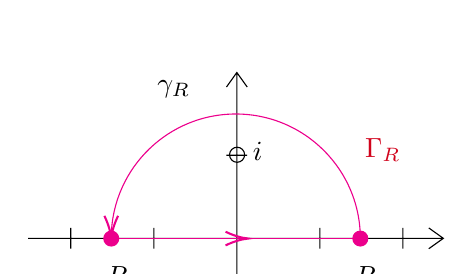
\begin{tikzpicture}[x=0.75pt,y=0.75pt,yscale=-1,xscale=1]
    %uncomment if require: \path (0,300); %set diagram left start at 0, and has height of 300
    
    %Shape: Axis 2D [id:dp3985790093437118] 
    \draw  (50,149.89) -- (250,149.89)(150.51,70) -- (150.51,170) (243,144.89) -- (250,149.89) -- (243,154.89) (145.51,77) -- (150.51,70) -- (155.51,77) (190.51,144.89) -- (190.51,154.89)(230.51,144.89) -- (230.51,154.89)(110.51,144.89) -- (110.51,154.89)(70.51,144.89) -- (70.51,154.89)(145.51,109.89) -- (155.51,109.89) ;
    \draw   ;
    %Straight Lines [id:da2085138625465428] 
    \draw [color=magenta  ,draw opacity=1 ]   (90,150) -- (210,150) ;
    \draw [shift={(210,150)}, rotate = 0] [color=magenta  ,draw opacity=1 ][fill=magenta  ,fill opacity=1 ][line width=0.75]      (0, 0) circle [x radius= 3.35, y radius= 3.35]   ;
    \draw [shift={(156,150)}, rotate = 180] [color=magenta  ,draw opacity=1 ][line width=0.75]    (10.93,-3.29) .. controls (6.95,-1.4) and (3.31,-0.3) .. (0,0) .. controls (3.31,0.3) and (6.95,1.4) .. (10.93,3.29)   ;
    \draw [shift={(90,150)}, rotate = 0] [color=magenta  ,draw opacity=1 ][fill=magenta  ,fill opacity=1 ][line width=0.75]      (0, 0) circle [x radius= 3.35, y radius= 3.35]   ;
    %Shape: Arc [id:dp46543149744952506] 
    \draw  [draw opacity=0] (89.99,150) .. controls (89.99,116.86) and (116.86,89.99) .. (150,89.99) .. controls (183.14,89.99) and (210.01,116.86) .. (210.01,150) -- (150,150) -- cycle ; \draw [color=magenta  ,draw opacity=1 ]   (90.04,147.53) .. controls (91.33,115.53) and (117.68,89.99) .. (150,89.99) .. controls (183.14,89.99) and (210.01,116.86) .. (210.01,150) ;  \draw [shift={(89.99,150)}, rotate = 270] [color=magenta  ,draw opacity=1 ][line width=0.75]    (10.93,-3.29) .. controls (6.95,-1.4) and (3.31,-0.3) .. (0,0) .. controls (3.31,0.3) and (6.95,1.4) .. (10.93,3.29)   ;
    %Shape: Circle [id:dp5979229833068613] 
    \draw   (147,109.63) .. controls (147,107.62) and (148.62,106) .. (150.63,106) .. controls (152.63,106) and (154.26,107.62) .. (154.26,109.63) .. controls (154.26,111.63) and (152.63,113.26) .. (150.63,113.26) .. controls (148.62,113.26) and (147,111.63) .. (147,109.63) -- cycle ;
    
    % Text Node
    \draw (76,162.4) node [anchor=north west][inner sep=0.75pt]    {$-R$};
    % Text Node
    \draw (206,162.4) node [anchor=north west][inner sep=0.75pt]    {$R$};
    % Text Node
    \draw (111,72.4) node [anchor=north west][inner sep=0.75pt]    {$\gamma _{R}$};
    % Text Node
    \draw (157,102.4) node [anchor=north west][inner sep=0.75pt]    {$i$};
    % Text Node
    \draw (211,100.4) node [anchor=north west][inner sep=0.75pt]    {$\textcolor[rgb]{0.82,0.01,0.11}{\Gamma _{R}}$};
    
    
    \end{tikzpicture}
    \]
Since $i$ is a pole enclosed in $\Gamma_R$, the residue theorem implies \(\int_{\Gamma_{R}}f(z)\d z=\,2\pi i\,\Res (f,i)\). By \cref{residue-formula}, \[\Res (f,i)=\operatorname*{lim}_{z\rightarrow i}(z-i)f(z)=\operatorname*{lim}_{z\rightarrow i}\frac{e^{i a z}}{(z+i)}=\frac{e^{-a}}{2i}\] so it follows that 
\[\rt{\int_{-R}^{R}{\frac{e^{i a x}}{1+x^{2}}}\d x}+\bt{\int_{\gamma_{R}}{\frac{e^{i a z}}{1+z^{2}}}\d z}=2\pi i\,\Res (f,i)=\pi e^{-a}\]

We look at $\bt{\int_{\gamma_{R}}{\frac{e^{i a z}}{1+z^{2}}}\d z}$. If $z=x+i y$ is on $\gamma_R$, then $y \geq 0$ and hence (since $a>0$):
\[\begin{aligned}
    \left|\bt{\int_{\gamma_{R}}{\frac{e^{i a z}}{1+z^{2}}}\d z}\right| & =\left|\int_{\gamma_R} \frac{e^{i a z}}{1+z^2} \d z\right| \\
    & \leq \pi R \sup _{z \in \gamma_R} \frac{\left|e^{i a z}\right|}{\left|1+z^2\right|} &&\text{by upper bound over length of curve}\\
    & \leq \pi R \sup _{x+i y \in \gamma_R} \frac{e^{-a y}}{R^2-1} &&\text{since }|e^{iax}|=1\\
    & =\frac{\pi R}{R^2-1}
    \end{aligned}\]
which tends to zero as $R \rightarrow \infty$.
Let $R \rightarrow \infty$ and get \[\rt{\int_{-\infty}^{\infty} \frac{e^{i a x}}{1+x^2} \d x}=\pi e^{-a}\] Thus the real part would be our answer \[\int_{-\infty}^{\infty} \frac{\cos a x}{1+x^2} d x=\pi e^{-a}\]

\section{Residue theory}
\subsection{Index, aka. winding number of a curve}
\defn Let $\gamma$ be a closed, piecewise $C^1$ curve and $z_0\notin \gamma$. The \textbf{index} (also called the \textbf{winding number}\sidenote{Number of counterclockwise loop-arounds}) of $\gamma$ with respect to $z_0$ is \[I(\gamma;z_0)=\frac{1}{2\pi i}\int_{\gamma}\frac{\d z}{z-z_0}\]

\rmk If the curve $\gamma:[a,b]\to \C$ is parameterized on $t$, and $\gamma(a)=\gamma(b)$ (closed), then let $z=\gamma(t), \d z=\gamma'(t)\d t$. Then we have \[I(\gamma;z_0)=\frac{1}{2\pi i}\int_{\gamma}\frac{\d z}{z-z_0} = \frac{1}{2\pi i}\int_{a}^{b}\frac{\gamma'(t)\d t}{\gamma(t)-z_0}\]

\begin{lemma}
    If $\gamma$ is a closed curve and $z_0\notin \gamma$, then $I(\gamma;z_0)\in \Z$.
\end{lemma}
\begin{proof}
    Parameterize $\gamma$ as above using $s$. Then \[\frac{1}{2\pi i}\int_{\gamma}\frac{\d z}{z-z_0} = \frac{1}{2\pi i}\int_{a}^{b}\frac{\gamma'(s)\d s}{\gamma(s)-z_0}\]
    Define \[g(t)=\int_{a}^{t}\frac{\gamma'(s)\d s}{\gamma(s)-z_0}\]
    Since $\gamma$ is \underline{piecewise}, by FTC, we have \[\rt{g'(t)=\frac{\gamma'(t)}{\gamma(t)-z_0}}\] for all but finitely many $t\in[a,b]$. Thus, \begin{align*}
        \frac{\d}{\d t}\left(e^{-g(t)}(\gamma(t)-z_0)\right) &= e^{-g(t)}\gamma'(t)-\rt{g'(t)}e^{-g(t)}(\gamma(t)-z_0)\\
        &= \gt{e^{-g(t)}\gamma'(t)}-\frac{\gt{\gamma'(t)}}{\bt{\gamma(t)-z_0}}\gt{e^{-g(t)}}(\bt{\gamma(t)-z_0})\\
        &= 0
    \end{align*}
    for all $t$ where $g'(t)$ exists. Therefore, $e^{-g(t)}(\gamma(t)-z_0)$ is piecewise constant. But this function is also \underline{continuous}, so it's constant! Therefore:
    \[e^{-g(b)}(\bt{\gamma(b)-z_0}) = e^{-g(a)}(\bt{\gamma(a)-z_0})\]
    The \bt{blue} terms are the same since $\gamma(a)=\gamma(b)$. Therefore, $e^{-g(b)}=e^{-g(a)}=e^0=1$ since $g(a)=0$.

    Hence, $g(b)=2\pi i n$ for some $n\in \Z$. Thus:\[I(\gamma;z_0)=\frac{1}{2\pi i}\int_{\gamma}\frac{\d z}{z-z_0} = \frac{1}{2\pi i}g(b) = n\in \Z\]
\end{proof}

\rmk Winding number essentially tracks the change of argument when the curve is traversed.
\[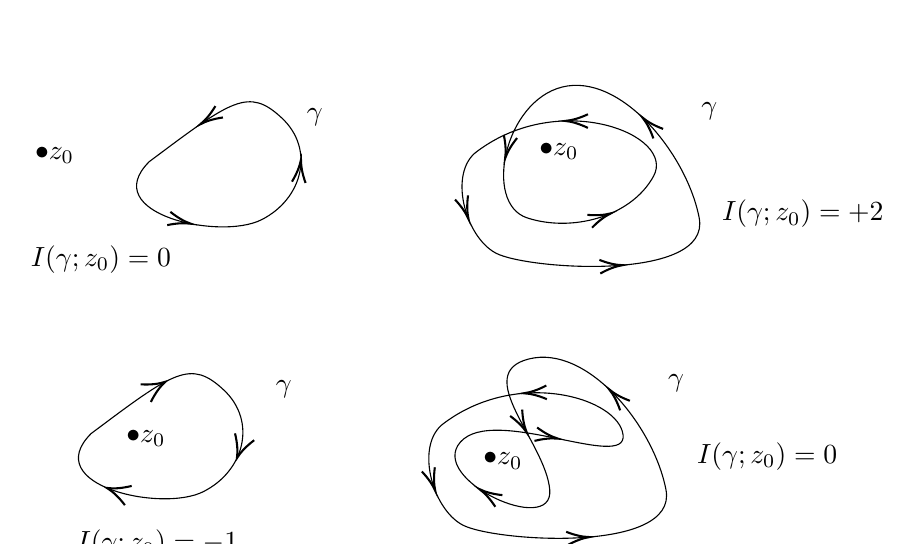
\begin{tikzpicture}[x=0.75pt,y=0.75pt,yscale=-1,xscale=1]
    %uncomment if require: \path (0,300); %set diagram left start at 0, and has height of 300
    
    %Curve Lines [id:da3037232848478386] 
    \draw    (88.26,49.14) .. controls (128.26,19.14) and (136.26,13.14) .. (152.26,28.14) .. controls (168.26,43.14) and (162.26,67.14) .. (142.26,77.14) .. controls (122.26,87.14) and (63.26,74.14) .. (88.26,49.14) -- cycle ;
    \draw [shift={(112.88,31.1)}, rotate = 326.5] [color=black  ][line width=0.75]    (10.93,-3.29) .. controls (6.95,-1.4) and (3.31,-0.3) .. (0,0) .. controls (3.31,0.3) and (6.95,1.4) .. (10.93,3.29)   ;
    \draw [shift={(161.41,48.16)}, rotate = 95.58] [color=black  ][line width=0.75]    (10.93,-3.29) .. controls (6.95,-1.4) and (3.31,-0.3) .. (0,0) .. controls (3.31,0.3) and (6.95,1.4) .. (10.93,3.29)   ;
    \draw [shift={(108.36,79)}, rotate = 193.37] [color=black  ][line width=0.75]    (10.93,-3.29) .. controls (6.95,-1.4) and (3.31,-0.3) .. (0,0) .. controls (3.31,0.3) and (6.95,1.4) .. (10.93,3.29)   ;
    %Curve Lines [id:da8924673024013423] 
    \draw    (246.26,44.14) .. controls (286.26,14.14) and (342.26,36.14) .. (331.26,56.14) .. controls (320.26,76.14) and (291.26,83.14) .. (270.26,76.14) .. controls (249.26,69.14) and (259.26,20.14) .. (287.26,13.14) .. controls (315.26,6.14) and (347.26,45.14) .. (353.26,76.14) .. controls (359.26,107.14) and (270.26,101.14) .. (255.26,93.14) .. controls (240.26,85.14) and (232.26,54.14) .. (246.26,44.14) -- cycle ;
    \draw [shift={(288.72,29.47)}, rotate = 0.38] [color=black  ][line width=0.75]    (10.93,-3.29) .. controls (6.95,-1.4) and (3.31,-0.3) .. (0,0) .. controls (3.31,0.3) and (6.95,1.4) .. (10.93,3.29)   ;
    \draw [shift={(310.76,73.98)}, rotate = 159.54] [color=black  ][line width=0.75]    (10.93,-3.29) .. controls (6.95,-1.4) and (3.31,-0.3) .. (0,0) .. controls (3.31,0.3) and (6.95,1.4) .. (10.93,3.29)   ;
    \draw [shift={(259.76,47.58)}, rotate = 283.56] [color=black  ][line width=0.75]    (10.93,-3.29) .. controls (6.95,-1.4) and (3.31,-0.3) .. (0,0) .. controls (3.31,0.3) and (6.95,1.4) .. (10.93,3.29)   ;
    \draw [shift={(325.89,27.79)}, rotate = 45.62] [color=black  ][line width=0.75]    (10.93,-3.29) .. controls (6.95,-1.4) and (3.31,-0.3) .. (0,0) .. controls (3.31,0.3) and (6.95,1.4) .. (10.93,3.29)   ;
    \draw [shift={(316.31,98.97)}, rotate = 176.13] [color=black  ][line width=0.75]    (10.93,-3.29) .. controls (6.95,-1.4) and (3.31,-0.3) .. (0,0) .. controls (3.31,0.3) and (6.95,1.4) .. (10.93,3.29)   ;
    \draw [shift={(242.13,76.76)}, rotate = 252.08] [color=black  ][line width=0.75]    (10.93,-3.29) .. controls (6.95,-1.4) and (3.31,-0.3) .. (0,0) .. controls (3.31,0.3) and (6.95,1.4) .. (10.93,3.29)   ;
    %Curve Lines [id:da4265358877348766] 
    \draw    (60.26,180.14) .. controls (100.26,150.14) and (108.26,144.14) .. (124.26,159.14) .. controls (140.26,174.14) and (134.26,198.14) .. (114.26,208.14) .. controls (94.26,218.14) and (35.26,205.14) .. (60.26,180.14) -- cycle ;
    \draw [shift={(96.08,155.14)}, rotate = 149.89] [color=black  ][line width=0.75]    (10.93,-4.9) .. controls (6.95,-2.3) and (3.31,-0.67) .. (0,0) .. controls (3.31,0.67) and (6.95,2.3) .. (10.93,4.9)   ;
    \draw [shift={(130.55,191.94)}, rotate = 289.75] [color=black  ][line width=0.75]    (10.93,-4.9) .. controls (6.95,-2.3) and (3.31,-0.67) .. (0,0) .. controls (3.31,0.67) and (6.95,2.3) .. (10.93,4.9)   ;
    \draw [shift={(67.9,206.3)}, rotate = 19.51] [color=black  ][line width=0.75]    (10.93,-4.9) .. controls (6.95,-2.3) and (3.31,-0.67) .. (0,0) .. controls (3.31,0.67) and (6.95,2.3) .. (10.93,4.9)   ;
    %Curve Lines [id:da7106931224469695] 
    \draw    (230.26,175.14) .. controls (266,148.34) and (314.51,163.05) .. (316.59,180.75) .. controls (318.67,198.45) and (254.26,166.14) .. (238.26,184.14) .. controls (222.26,202.14) and (283.26,230.14) .. (281.26,207.14) .. controls (279.26,184.14) and (243.26,151.14) .. (271.26,144.14) .. controls (299.26,137.14) and (331.26,176.14) .. (337.26,207.14) .. controls (343.26,238.14) and (254.26,232.14) .. (239.26,224.14) .. controls (224.26,216.14) and (216.26,185.14) .. (230.26,175.14) -- cycle ;
    \draw [shift={(268.81,160.68)}, rotate = 357.68] [color=black  ][line width=0.75]    (10.93,-3.29) .. controls (6.95,-1.4) and (3.31,-0.3) .. (0,0) .. controls (3.31,0.3) and (6.95,1.4) .. (10.93,3.29)   ;
    \draw [shift={(285.27,182.55)}, rotate = 191.28] [color=black  ][line width=0.75]    (10.93,-3.29) .. controls (6.95,-1.4) and (3.31,-0.3) .. (0,0) .. controls (3.31,0.3) and (6.95,1.4) .. (10.93,3.29)   ;
    \draw [shift={(247.41,206.88)}, rotate = 31.32] [color=black  ][line width=0.75]    (10.93,-3.29) .. controls (6.95,-1.4) and (3.31,-0.3) .. (0,0) .. controls (3.31,0.3) and (6.95,1.4) .. (10.93,3.29)   ;
    \draw [shift={(270.24,179.71)}, rotate = 241.88] [color=black  ][line width=0.75]    (10.93,-3.29) .. controls (6.95,-1.4) and (3.31,-0.3) .. (0,0) .. controls (3.31,0.3) and (6.95,1.4) .. (10.93,3.29)   ;
    \draw [shift={(309.89,158.79)}, rotate = 45.62] [color=black  ][line width=0.75]    (10.93,-3.29) .. controls (6.95,-1.4) and (3.31,-0.3) .. (0,0) .. controls (3.31,0.3) and (6.95,1.4) .. (10.93,3.29)   ;
    \draw [shift={(300.31,229.97)}, rotate = 176.13] [color=black  ][line width=0.75]    (10.93,-3.29) .. controls (6.95,-1.4) and (3.31,-0.3) .. (0,0) .. controls (3.31,0.3) and (6.95,1.4) .. (10.93,3.29)   ;
    \draw [shift={(226.13,207.76)}, rotate = 252.08] [color=black  ][line width=0.75]    (10.93,-3.29) .. controls (6.95,-1.4) and (3.31,-0.3) .. (0,0) .. controls (3.31,0.3) and (6.95,1.4) .. (10.93,3.29)   ;
    
    % Text Node
    \draw (32,41) node [anchor=north west][inner sep=0.75pt]   [align=left] {$\displaystyle \bullet z_{0}$};
    % Text Node
    \draw (163,22.4) node [anchor=north west][inner sep=0.75pt]    {$\gamma $};
    % Text Node
    \draw (30,88.4) node [anchor=north west][inner sep=0.75pt]    {$I( \gamma ;z_{0}) =0$};
    % Text Node
    \draw (275,39) node [anchor=north west][inner sep=0.75pt]   [align=left] {$\displaystyle \bullet z_{0}$};
    % Text Node
    \draw (353,19.4) node [anchor=north west][inner sep=0.75pt]    {$\gamma $};
    % Text Node
    \draw (363,66.4) node [anchor=north west][inner sep=0.75pt]    {$I( \gamma ;z_{0}) =+2$};
    % Text Node
    \draw (76,177) node [anchor=north west][inner sep=0.75pt]   [align=left] {$\displaystyle \bullet z_{0}$};
    % Text Node
    \draw (148,153.4) node [anchor=north west][inner sep=0.75pt]    {$\gamma $};
    % Text Node
    \draw (52,225.4) node [anchor=north west][inner sep=0.75pt]    {$I( \gamma ;z_{0}) =-1$};
    % Text Node
    \draw (248,188) node [anchor=north west][inner sep=0.75pt]   [align=left] {$\displaystyle \bullet z_{0}$};
    % Text Node
    \draw (337,150.4) node [anchor=north west][inner sep=0.75pt]    {$\gamma $};
    % Text Node
    \draw (351,183.4) node [anchor=north west][inner sep=0.75pt]    {$I( \gamma ;z_{0}) =0$};
    
    
    \end{tikzpicture}
    \]

\subsection{Simply connected domains}
\defn A region $\reg$ is \textbf{simply connected} if it has no holes. In other words: \begin{enumerate}[label=(\alph*)]
    \item $I(\gamma;z_0)=0$ for \textbf{every} closed curve $\gamma$ in $\reg$ and every $z_0\notin \reg$. 
    \item Every closed curve $\gamma$ in $\reg$ is \textbf{homotopic}\sidenote{homotopic means can be continuously deformed without passing outside $\reg$} to a point in $\reg$.
\end{enumerate}

Recall \cref{cauchys-take1}. We can now extend beyond simple curves: 
\begin{theorem}[Cauchy's, for simply connected domains]\label[theorem]{cauchys-simply-connected}
    If $\reg$ is \textbf{simply connected}, $f$ is analytic on $\reg$, then $\int_{\gamma}f(z)\d z=0$ for any closed curve $\gamma$ in $\reg$.
    \[\begin{tikzpicture}[x=0.75pt,y=0.75pt,yscale=-0.8,xscale=.8]
        %uncomment if require: \path (0,300); %set diagram left start at 0, and has height of 300
        
        %Curve Lines [id:da48836246897955626] 
        \draw    (106.26,135.14) .. controls (98.26,94.64) and (261.26,174.64) .. (276.26,167.64) .. controls (291.26,160.64) and (292.26,136.64) .. (273.26,123.64) .. controls (254.26,110.64) and (112.26,211.64) .. (106.26,135.14) -- cycle ;
        \draw [shift={(182.63,138.83)}, rotate = 18.82] [color=black  ][line width=0.75]    (10.93,-3.29) .. controls (6.95,-1.4) and (3.31,-0.3) .. (0,0) .. controls (3.31,0.3) and (6.95,1.4) .. (10.93,3.29)   ;
        \draw [shift={(287.27,152.15)}, rotate = 271.16] [color=black  ][line width=0.75]    (10.93,-3.29) .. controls (6.95,-1.4) and (3.31,-0.3) .. (0,0) .. controls (3.31,0.3) and (6.95,1.4) .. (10.93,3.29)   ;
        \draw [shift={(189.52,151.48)}, rotate = 159.72] [color=black  ][line width=0.75]    (10.93,-3.29) .. controls (6.95,-1.4) and (3.31,-0.3) .. (0,0) .. controls (3.31,0.3) and (6.95,1.4) .. (10.93,3.29)   ;
        %Shape: Polygon Curved [id:ds5031523676345244] 
        \draw  [dash pattern={on 4.5pt off 4.5pt}] (118.26,73.39) .. controls (145.26,45.39) and (227.51,58.79) .. (270.26,88.39) .. controls (313,118) and (324.26,166.39) .. (305.26,193.39) .. controls (286.26,220.39) and (227.26,207.39) .. (193.26,215.39) .. controls (159.26,223.39) and (107.26,220.39) .. (91.26,176.39) .. controls (75.26,132.39) and (91.26,101.39) .. (118.26,73.39) -- cycle ;
        
        % Text Node
        \draw (155,64.4) node [anchor=north west][inner sep=0.75pt]  [xscale=0.8,yscale=0.8]  {$\Omega $};
        
        
        \end{tikzpicture}
        \]
\end{theorem}

\addlink{Simply connected iff. antiderivative exists}
\begin{theorem}
    A region $\reg$ is \textbf{simply connected} \ifnif every analytic function $f:\reg\to\C$ has an \textbf{antiderivative} on $\reg$.
\end{theorem}
\begin{proof}We proved in \cref{convex-antiderivative} that every analytic function $f:\reg\to\C$ on a \textit{convex} $\reg$ has an antiderivative. We adapt the proof.
    \begin{itemize}[align = left]
        \item[$(\implies)$] \[\begin{tikzpicture}[x=0.75pt,y=0.75pt,yscale=-1,xscale=1]
            %uncomment if require: \path (0,300); %set diagram left start at 0, and has height of 300
            
            %Shape: Polygon Curved [id:ds5031523676345244] 
            \draw  [dash pattern={on 4.5pt off 4.5pt}] (104.26,121.89) .. controls (131.26,93.89) and (137.51,31.29) .. (180.26,60.89) .. controls (223,90.5) and (304.26,196.89) .. (285.26,223.89) .. controls (266.26,250.89) and (197.26,172.39) .. (164.26,181.89) .. controls (131.26,191.39) and (82.26,235.39) .. (66.26,191.39) .. controls (50.26,147.39) and (77.26,149.89) .. (104.26,121.89) -- cycle ;
            %Curve Lines [id:da4418491251136758] 
            \draw [color=magenta  ,draw opacity=1 ]   (104.26,159.89) .. controls (144.26,129.89) and (189.26,108.89) .. (223,138) ;
            %Curve Lines [id:da5888793969301926] 
            \draw [color=cyan  ,draw opacity=1 ]   (104.26,159.89) .. controls (125.26,176.89) and (217,165) .. (223,138) ;
            %Straight Lines [id:da9116430727041929] 
            \draw    (206,139) -- (270.52,101.89) ;
            \draw [shift={(272.26,100.89)}, rotate = 150.09] [color=black  ][line width=0.75]    (10.93,-3.29) .. controls (6.95,-1.4) and (3.31,-0.3) .. (0,0) .. controls (3.31,0.3) and (6.95,1.4) .. (10.93,3.29)   ;
            
            % Text Node
            \draw (155,64.4) node [anchor=north west][inner sep=0.75pt]  [xscale=0.8,yscale=0.8]  {$\Omega $};
            % Text Node
            \draw (223,68) node [anchor=north west][inner sep=0.75pt]  [xscale=0.8,yscale=0.8] [align=left] {No points of $\displaystyle \Omega ^{c}$ here!};
            % Text Node
            \draw (135,112.4) node [anchor=north west][inner sep=0.75pt]  [color=magenta  ,opacity=1 ,xscale=0.8,yscale=0.8]  {$\gamma _{1}$};
            % Text Node
            \draw (210,154.4) node [anchor=north west][inner sep=0.75pt]  [xscale=0.8,yscale=0.8]  {$\textcolor{cyan}{\gamma _{2}}$};
            
            
            \end{tikzpicture}
            \]
            Then use \cref{cauchys-take2-deform}.
        \item[$(\impliedby)$] Suppose BWOC that $\reg$ is \textbf{not} simply connected. Then there is a $z_0\in \reg^c$ and $\gamma$ a closed curve in $\reg$ such that $I(\gamma;z_0)\neq 0$. Then \(f(z)=\frac{1}{z-z_0}\) does not have an antiderivative on $\reg$. 
    \end{itemize}
\end{proof}

\addlink{Existence of log for non-vanishing functions}
\begin{theorem}
    If $\reg$ is simply connected and $f:\reg\to\C$ is analytic and \textbf{never 0}, then there is an analytic $g:\reg\to \C$ such that $f=e^g$. That is, it's got a log!
\end{theorem}
\begin{proof}
    The function $f'/f$ is analytic on $\reg$, thus it has an antiderivative $F$ on $\reg$. Since \[(f e^{-F})^{\prime}=f^{\prime}e^{-F}-F^{\prime}f e^{-F}=f^{\prime}e^{-F}-f^{\prime}e^{-F}=0\]it follows that $fe^{-F} =c$ for some constant $c$. Thus, $g=\log c+F$ (we may choose any fixed branch of $\log c$).
\end{proof}

\addlink{Residue theorem (general version)}
\begin{theorem}[Residue, general case]
    Let $\reg$ be a simply-connected region and let $z_1,z_2,\dots,z_n\in \reg$ be distinct. If $f:\reg\backslash\{z_{1},z_{2},\cdot\cdot\cdot,z_{n}\}\to\mathbb{C}$ is analytic and $\gamma$ is a closed curve in $\reg$ that
    passes through no $z_i$, then
    \[\frac{1}{2\pi i}\int_{\gamma}f(\zeta)\,d\zeta=\sum_{j=1}^{n}\Res (f;z_{j})I(\gamma,z_{j})\]
\end{theorem}

\subsection{The argument principle}
Suppose $f: \Omega \rightarrow \mathbb{C}$ is analytic and has zeros only at $z_1, z_2, \ldots, z_n \in \Omega$ (repeated according to multiplicity). Write
\[f(z)=\left(z-z_1\right)\left(z-z_2\right) \cdots\left(z-z_n\right) g(z)\]
where $g(z)$ is analytic and nonvanishing on $\Omega$. The product formula for derivatives implies
\[
\begin{aligned}
& f^{\prime}(z)=\left(z-z_2\right)\left(z-z_3\right) \cdots\left(z-z_n\right) g(z)+\left(z-z_1\right)\left(z-z_3\right) \cdots\left(z-z_n\right) g(z)+\cdots \\
&+\left(z-z_1\right)\left(z-z_2\right) \cdots\left(z-z_{n-1}\right) g(z)+\left(z-z_1\right)\left(z-z_2\right) \cdots\left(z-z_n\right) g^{\prime}(z) .
\end{aligned}
\]

Divide by $f(z)$ and obtain the \uline{logarithmic derivative of $f$}\sidenote{Since $(\log f)' = f'/f$}:
\[\rt{\frac{f^{\prime}(z)}{f(z)}}=\frac{1}{z-z_1}+\frac{1}{z-z_2}+\cdots+\frac{1}{z-z_n}+\frac{g^{\prime}(z)}{g(z)} \]

If $\gamma$ is a simple closed curve\sidenote{a simple closed curve can only envelope a finite amount of zeros!} in $\Omega$ whose interior lies in $\Omega$ and which contains each $z_i$ in its interior, then
\[\begin{aligned}
    \frac{1}{2 \pi i} \int_\gamma \rt{\frac{f^{\prime}(z)}{f(z)}} \d z & =\bt{\sum_{k=1}^n \frac{1}{2 \pi i} \int_\gamma \frac{\d z}{z-z_k}}+\gt{\frac{1}{2 \pi i} \int_\gamma \frac{g^{\prime}(z)}{g(z)} \d z} \\
    &= \sum_{k=1}^{n}I(\gamma;z_k) + \gt{0}\\
    & =\left(\sum_{k=1}^n 1\right)+0 \\
    & =n 
    \end{aligned}\]

The \gt{final integral} vanishes by Cauchy's theorem since $g^{\prime} / g$ is analytic on $\Omega$. Integrating the logarithmic derivative $\rt{f^{\prime} / f}$ of an analytic function $f$ around a closed curve $\gamma$ \uline{counts the number of zeros} of $f$, repeated according to multiplicity, inside of $\gamma$.

\theorem[The Argument Principle] Let $\Omega$ be a region in $\mathbb{C}$ and let $\gamma$ be a simple closed curve in $\Omega$ with its interior in $\Omega$. If $f:\Omega\to\mathbb{C}$ is analytic and has no zeros on $\gamma$, then the \underline{number of zeros} $Z_{f}(\gamma)$ of $f$, repeated according to multiplicity, in the interior of $\gamma$ is finite and is given by
    \[Z_{f}(\gamma)=\frac{1}{2\pi i}\int_{\gamma}\frac{f^{\prime}(z)}{f(z)}\d z\]
\begin{proof}
    In light of the preceding discussion, we only need to show that $f$ has only finitely many zeros inside of $\gamma$. Let $G$ denote the union of $\gamma$ and its interior. Since $G$ is closed and bounded, it is compact. If $f$ had infinitely many distinct zeros $z_{n}$ inside of $\gamma$, these would have an accumulation point in $G\subseteq\Omega$. The identity theorem would imply that $f$ is identically zero on $\Omega$, which contradicts the hypothesis that $f$ does not vanish on $\gamma$.
\end{proof}

\rmk Why \textit{argument} principle? Let $\gamma:[a,b]\rightarrow\mathbb{C}$ be a parametrization and consider the curve $f\circ\gamma:[a,b]\rightarrow\mathbb{C}$. The following computation shows that the number of zeros of $f$ inside $\gamma$ equals the winding number of $f\circ\gamma$ with respect to the origin:
\begin{align*}
    Z_{f}(\gamma)&=\frac{1}{2\pi i}\int_{\gamma}\frac{f^{\prime}(z)}{f(z)}\d z\\
    &=\frac{1}{2\pi i}\int_{a}^{b}\frac{f^{\prime}(\gamma(t))\gamma^{\prime}(t)\d t}{f(\gamma(t))}\\
    &=\frac{1}{2\pi i}\int_{f\circ\gamma}\frac{\d \zeta}{\zeta-0}\\
    &=I(f\circ\gamma;0)
\end{align*}

in which $\zeta=f(\gamma(t))$ and $d\zeta=f^{\prime}(\gamma(t))\gamma^{\prime}(t)\,dt$ by the chain rule.

It allows computers to compute roots with great ease. As soon as we have an error $<\frac{1}{2}$ we are done.

\[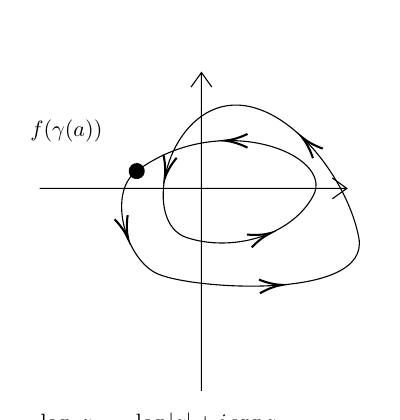
\begin{tikzpicture}[x=0.75pt,y=0.75pt,yscale=-1,xscale=1]
    %uncomment if require: \path (0,300); %set diagram left start at 0, and has height of 300
    
    %Curve Lines [id:da5005822895298122] 
    \draw    (179.26,108.14) .. controls (219.26,78.14) and (275.26,100.14) .. (264.26,120.14) .. controls (253.26,140.14) and (224.26,147.14) .. (203.26,140.14) .. controls (182.26,133.14) and (192.26,84.14) .. (220.26,77.14) .. controls (248.26,70.14) and (280.26,109.14) .. (286.26,140.14) .. controls (292.26,171.14) and (203.26,165.14) .. (188.26,157.14) .. controls (173.26,149.14) and (165.26,118.14) .. (179.26,108.14) -- cycle ;
    \draw [shift={(221.72,93.47)}, rotate = 0.38] [color=black  ][line width=0.75]    (10.93,-3.29) .. controls (6.95,-1.4) and (3.31,-0.3) .. (0,0) .. controls (3.31,0.3) and (6.95,1.4) .. (10.93,3.29)   ;
    \draw [shift={(243.76,137.98)}, rotate = 159.54] [color=black  ][line width=0.75]    (10.93,-3.29) .. controls (6.95,-1.4) and (3.31,-0.3) .. (0,0) .. controls (3.31,0.3) and (6.95,1.4) .. (10.93,3.29)   ;
    \draw [shift={(192.76,111.58)}, rotate = 283.56] [color=black  ][line width=0.75]    (10.93,-3.29) .. controls (6.95,-1.4) and (3.31,-0.3) .. (0,0) .. controls (3.31,0.3) and (6.95,1.4) .. (10.93,3.29)   ;
    \draw [shift={(258.89,91.79)}, rotate = 45.62] [color=black  ][line width=0.75]    (10.93,-3.29) .. controls (6.95,-1.4) and (3.31,-0.3) .. (0,0) .. controls (3.31,0.3) and (6.95,1.4) .. (10.93,3.29)   ;
    \draw [shift={(249.31,162.97)}, rotate = 176.13] [color=black  ][line width=0.75]    (10.93,-3.29) .. controls (6.95,-1.4) and (3.31,-0.3) .. (0,0) .. controls (3.31,0.3) and (6.95,1.4) .. (10.93,3.29)   ;
    \draw [shift={(175.13,140.76)}, rotate = 252.08] [color=black  ][line width=0.75]    (10.93,-3.29) .. controls (6.95,-1.4) and (3.31,-0.3) .. (0,0) .. controls (3.31,0.3) and (6.95,1.4) .. (10.93,3.29)   ;
    \draw [shift={(179.26,108.14)}, rotate = 323.13] [color=black  ][fill=black  ][line width=0.75]      (0, 0) circle [x radius= 3.35, y radius= 3.35]   ;
    %Shape: Axis 2D [id:dp5544761970205885] 
    \draw  (132.49,116.48) -- (280.51,116.48)(210.45,60.64) -- (210.45,214) (273.51,111.48) -- (280.51,116.48) -- (273.51,121.48) (205.45,67.64) -- (210.45,60.64) -- (215.45,67.64)  ;
    
    % Text Node
    \draw (127,82.4) node [anchor=north west][inner sep=0.75pt]  [xscale=0.8,yscale=0.8]  {$f( \gamma ( a))$};
    % Text Node
    \draw (132,223.4) node [anchor=north west][inner sep=0.75pt]  [xscale=0.8,yscale=0.8]  {$\log \ z\ =\ \log |z|+i\arg z$};
    
    
    \end{tikzpicture}
    \]  

\addlink{Root counting formula}
\begin{corollary}[Root counting formula]
    If $f:\reg\to\C$ is analytic and $\gamma$ is a simple closed curve in $\gamma$ with its interior in $\reg$ such that $f(z)\neq w$ on $\gamma$, then the number of roots of $f(z)=w$ inside $\gamma$ (with multiplicity) is $$Z_{f(z)-w}(\gamma)=\frac{1}{2\pi i}\int_{\gamma}\frac{f^{\prime}(z)}{f(z)-w}\d z$$
\end{corollary}

\eg Consider the function \[f(z)=z\left(\frac{z+\frac{1}{2}}{1+\frac{1}{2}\,z}\right)\left(\frac{z-\frac{3}{4}}{1-\frac{3}{4}\,z}\right)\left(\frac{z-\frac{4\,i}{5}}{1+\frac{4\,i}{5}\,z}\right)\] Being a product of disk automorphisms, $f$ maps $\D\to\D$. It has roots $0,\frac{-1}{2}, \frac{4i}{5}, \frac{3}{4}$. We could observe the increment of winding number corresponding to how many times zeros are included.
\drawing{0.8\linewidth}{image-8.png}

\subsection{Rouch\'e's theorem}

\begin{theorem}[Rouch\'e's] \label[theorem]{rouches-theorem}
    Let $f,g:\reg\to\C$ be analytic on $\reg$ and let $\gamma$ be a simple closed curve in $\reg$ that is homotopic to a point in $\reg$.
    If \(|f(z)-g(z)|<|f(z)|+|g(z)|\)\sidenote{observe that this is a ridiculously lenient hypothesis!} on $\gamma$,
    then $f,g$ have the same number of zeros (by multiplicity) inside $\gamma$.
\end{theorem}
\begin{proof}
    Note that the hypothesis implies that $f,g$ don't vanish on $\gamma$. Therefore, we can divide $g$ on both sides and get $\left|\frac{f}{g}-1\right|<\left|\frac{f}{g}\right|+1$ on $\gamma$. This inequality is violated whenever $f/g$ is a nonpositive real number $(\leq 0)$ on $\gamma$.

    Thus, $f/g$ maps $\gamma$ into $\C\setminus (-\infty,0]$. If $\ell(z)$ is the principal branch of the logarithm\sidenote{Recall that the principal
    branch of the logarithm has
    domain $\C\setminus (-\infty,0]$}, then $\ell\left(\frac{f}{g}\right)$ is defined on $\gamma$, and we have the logarithmic derivative $$\frac{\d}{\d z}\ell \left(\frac{f}{g}\right)=\frac{(f/g)^{\prime}}{f/g}$$
    on some open set containing $\gamma$. The Fundamental Theorem of Calculus and the argument
    principle imply 
    \begin{align*}
        0&\stackrel{FTC}{=}\frac{1}{2\pi i}\int_{\gamma}\frac{(f(z)/g(z))^{\prime}}{f(z)/g(z)}\d z\\ 
        &=\frac{1}{2\pi i}\int_{\gamma}\left(\frac{f^{\prime}(z)g(z)-f(z)g^{\prime}(z)}{g(z)^{2}}\cdot\frac{g(z)}{f(z)}\right)\d z\\ 
        &=\frac{1}{2\pi i}\int_{\gamma}\left(\frac{f^{\prime}(z)}{f(z)}-\frac{g^{\prime}(z)}{g(z)}\right)\d z\\ 
        &=\rt{\frac{1}{2\pi i}\int_{\gamma}\frac{f^{\prime}(z)}{f(z)}\d z}-\bt{\frac{1}{2\pi i}\int_{\gamma}\frac{g^{\prime}(z)}{g(z)}\d z}\\ 
        &=\rt{Z_{f}(\gamma)}-\bt{Z_{g}(\gamma)}
    \end{align*}
\end{proof}

\addlink{Weak Rouch\'e's theorem}
\begin{corollary}[Weak Rouch\'e's]\label[corollary]{weak-rouches}
    Let $f,h:\Omega\to\mathbb{C}$ be analytic on $\Omega$ and $\gamma$ be a closed curve in $\Omega$ that is homotopic to a point in $\Omega$. If $|h(z)|<|f(z)|$\sidenote{think $h$ perturbs $f$ a little bit} for all $z\in\gamma$, then $f$ and $f+h$ have the same number of zeros (counted by multiplicity) inside of $\gamma$.
\end{corollary}
\begin{proof}
    If $z\in \gamma$, then $$\left|\left(f(z)+h(z)\right)-f(z)\right|=|h(z)|<\rt{|f(z)|\leq|f(z)+h(z)|+|f(z)|}.$$
    \rt{This} is a significant overestimation. Let $f+h$ be the $g$ in \cref{rouches-theorem} and obtain the result.
\end{proof}

\rmk How to think about \cref{weak-rouches}? Let $f(z)$ where $z\in \gamma$ be the position of a dog walker in a garden. Let 0 be a tree. Let $f(z)+h(z)$ denote the position of the dog on leash. The fact that $|h|<|f|$ means the leash is shorter than the distance from the walker to the origin. We observe that the dog cannot walk around the tree more times than the owner!

\subsubsection{Fundamental Theorem of Algebra}
\begin{corollary}[FTA]
    If $p$ is a polynomial of degree $n \geq 1$, then $p(z)$ has exactly $n$ roots in $\C$, counted according to multiplicity.
\end{corollary}
\begin{proof}
    If $p(z)=a_{n}z^{n}+a_{n-1}z^{n-1}+\cdots+a_{0}$ and $a_{n}\neq0$, then\sidenote{a polynomial is dominated by its leading term} \[\lim_{z\to\infty}\frac{p(z)}{a_{n}z^{n}}=1\]
    For sufficiently large $R>0$,
    $$|z|=R\quad\implies\quad\left|\frac{p(z)}{a_{n}z^{n}}-1\right|<1$$
    and hence   
    $$|z|=R\quad\implies\quad\left|\frac{p(z)}{f(z)}-\frac{a_{n}z^{n}}{g(z)}\right|<\left|\frac{a_{n}z^{n}}{g(z)}\right|.$$
    Weak Rouche's theorem (\cref{weak-rouches}) implies that $p(z)$ and $a_nz^{n}$ have the same number of zeros (namely $n$), counted according to multiplicities, inside any disk of sufficiently large radius.    
\end{proof}

\eg Consider the transcendental equation $e^{z}=3z^{n}$\sidenote{observe this is hard to solve by non-numerical methods}, in which $n$ is a positive integer. How many solutions does it have inside the unit circle?

Let $$f(z)=e^{z}-3z^{n}\qquad\text{and}\qquad g(z)=-3z^{n}$$ and note that $g$ has precisely $n$ zeros (counted by multiplicity) in $|z|<1$. 

For $|z|=1$,
$$|\underbrace{(e^{z}-3z^{n})}_{f(z)}-\underbrace{(-3z^{n})}_{g(z)}|=|e^{z}|=e^{\re z}\leq e<3=|\underbrace{-3z^{n}}_{g(z)}|\leq \underbrace{-3z^{n}}_{g(z)}| + \underbrace{e^{z}-3z^n}_{f(z)}|$$
Rouch\'e's theorem (\cref{rouches-theorem}) implies that $f$ has exactly $n$ roots inside the unit circle.

\rmk We can also use the argument principle to get $Z_f(\gamma)=I(f\circ \gamma; 0)$ and integrate numerically up to a precision of $1/2$, but Rouch\'e's theorem is certainly more computationally light.

\eg Consider

$$f(z)=z^{9}-8z^{2}+5.$$

Since $\deg f=9$ we do not expect to find its zeros in closed form.\sidenote{cf. Galois theory} 
However, we can use Rouch\'e's theorem to help locate their general whereabouts.

Since $f$ has real coefficients and odd degree, the \textbf{intermediate value theorem} implies that $f$ has at least one real root. Since $f$ has real coefficients, the non-real roots of $f$ must appear in complex conjugate pairs. Thus, $f$ has an odd number of real roots.

For $|z|=\frac{3}{2}$, \begin{align*}
    |\underbrace{z^{9}-8z^{2}+5}_{f}-\underbrace{z^{9}}_{g}|&=|8z^{2}-5|\\
    &\leq8(\tfrac{3}{2})^{2}+5\\
    &=23\\
    &<(\tfrac{3}{2})^{9}\quad(\approx38.44)\\
    &=\underbrace{|z^9|}_{g}
\end{align*}
Rouch\'e's theorem implies $f$ has 9 zeros (counted according to multiplicity) in $|z|<\frac{3}{2}$. By FTA, these are all roots of $f$.

Now we look at smaller regions to gauge the distribution of the roots of $f$.

For $|z|=1$,\sidenote{this $g$ has 2 roots} \begin{align*}
    |\underbrace{z^{9}-8z^{2}+5}_{f}\ -\ \underbrace{(-8z^{2}+5)}_{g}|&=|z^{9}|\\
    &=1<3\leq |\underbrace{-8z^{2}+5}_{g}|
\end{align*}
Rouch\'e's theorem implies $f$ has 2 zeros, counted by multiplicity, in $|z|<1$.

For $|z|=\frac{1}{2}$,\sidenote{this $g$ has 0 roots}\begin{align*}
    |\underbrace{z^{9}-8z^{2}+5}_{f}\ +\underbrace{-5}_{g}|&=|z^{9}-8z^{2}|\\
    &\leq|z|^{9}+8|z|^{2}\\
    &=\frac{1}{2^{9}}+2\\
    &<5=|\underbrace{-5}_{g}|
\end{align*}
Rouch\'e's theorem implies $f$ has no zeros in $|z|<\frac{1}{2}$.

\subsection{Local mapping theorem}
\begin{theorem}[Local mapping]
    Suppose that $f:\Omega\to\mathbb{C}$ is analytic and nonconstant. Let $z_{0}\in\Omega$ and let the value $w_{0}=f(z_{0})$ be assumed with multiplicity $n$\sidenote{$f(z)-w_{0}$ has a zero of order $n$ at $z_{0}$}. 
    
    For each sufficiently small $\delta>0$, there exists $\varepsilon>0$ such that $0<|w_{0}-w_{0}|<\varepsilon$ implies that $f$ assumes the value $w$ at exactly $n$ distinct points in $0<|z-z_{0}|<\delta$, each with multiplicity one.
    \[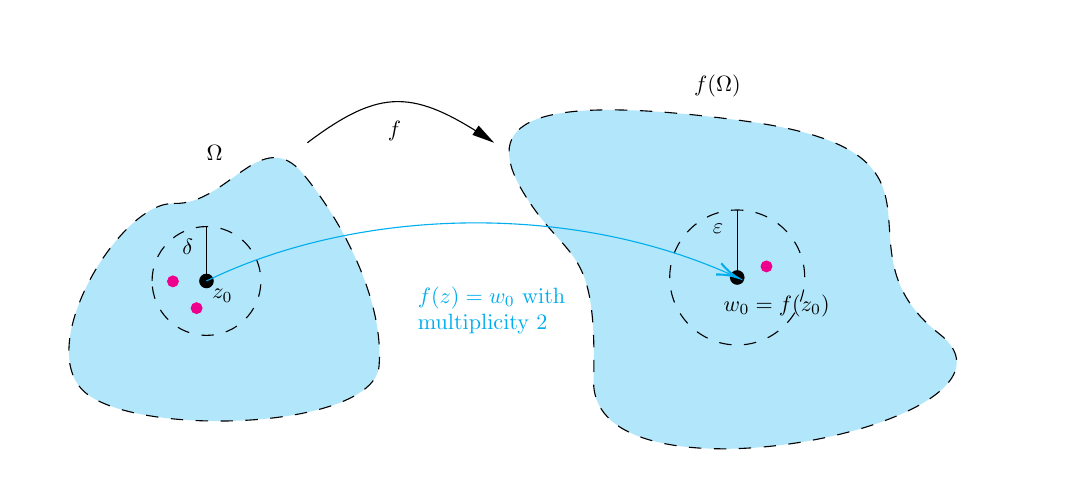
\begin{tikzpicture}[x=0.75pt,y=0.75pt,yscale=-.9,xscale=.9]
        %uncomment if require: \path (0,300); %set diagram left start at 0, and has height of 300
        
        %Shape: Polygon Curved [id:ds199380446597198] 
        \draw  [fill=cyan  ,fill opacity=0.3 ][dash pattern={on 4.5pt off 4.5pt}] (112.5,123.5) .. controls (141.5,124.5) and (159.5,80.5) .. (182,108) .. controls (204.5,135.5) and (224.91,176.75) .. (222.42,210.25) .. controls (219.92,243.75) and (99.59,248.75) .. (67.08,226.25) .. controls (34.58,203.75) and (83.5,122.5) .. (112.5,123.5) -- cycle ;
        %Shape: Polygon Curved [id:ds46424882675538726] 
        \draw  [fill=cyan  ,fill opacity=0.3 ][dash pattern={on 4.5pt off 4.5pt}] (301.25,120.25) .. controls (278.25,84.25) and (291.25,62.25) .. (417.25,79.25) .. controls (543.25,96.25) and (462.25,146.25) .. (522.25,193.25) .. controls (582.25,240.25) and (335.25,291.25) .. (337.25,218.25) .. controls (339.25,145.25) and (324.25,156.25) .. (301.25,120.25) -- cycle ;
        %Curve Lines [id:da3742131578130379] 
        \draw    (184,91) .. controls (223.6,61.3) and (240.91,62.23) .. (282.73,90.15) ;
        \draw [shift={(284,91)}, rotate = 213.92] [fill=black  ][line width=0.08]  [draw opacity=0] (12,-3) -- (0,0) -- (12,3) -- cycle    ;
        %Shape: Circle [id:dp6048852286733579] 
        \draw  [dash pattern={on 4.5pt off 4.5pt}] (100.87,165) .. controls (100.87,148.91) and (113.91,135.87) .. (130,135.87) .. controls (146.09,135.87) and (159.13,148.91) .. (159.13,165) .. controls (159.13,181.09) and (146.09,194.13) .. (130,194.13) .. controls (113.91,194.13) and (100.87,181.09) .. (100.87,165) -- cycle ;
        %Shape: Circle [id:dp9734988957299731] 
        \draw  [dash pattern={on 4.5pt off 4.5pt}] (378,163.13) .. controls (378,143.18) and (394.18,127) .. (414.13,127) .. controls (434.08,127) and (450.26,143.18) .. (450.26,163.13) .. controls (450.26,183.08) and (434.08,199.26) .. (414.13,199.26) .. controls (394.18,199.26) and (378,183.08) .. (378,163.13) -- cycle ;
        %Straight Lines [id:da4544217864520035] 
        \draw    (130,135.87) -- (130,165) ;
        \draw [shift={(130,165)}, rotate = 90] [color=black  ][fill=black  ][line width=0.75]      (0, 0) circle [x radius= 3.35, y radius= 3.35]   ;
        %Straight Lines [id:da37495890514322716] 
        \draw    (414.13,127) -- (414.13,163.13) ;
        \draw [shift={(414.13,163.13)}, rotate = 90] [color=black  ][fill=black  ][line width=0.75]      (0, 0) circle [x radius= 3.35, y radius= 3.35]   ;
        %Curve Lines [id:da6838529182425372] 
        \draw [color=cyan  ,draw opacity=1 ]   (130,165) .. controls (209.85,126.09) and (324.11,121.93) .. (412.79,162.51) ;
        \draw [shift={(414.13,163.13)}, rotate = 204.89] [color=cyan  ,draw opacity=1 ][line width=0.75]    (10.93,-3.29) .. controls (6.95,-1.4) and (3.31,-0.3) .. (0,0) .. controls (3.31,0.3) and (6.95,1.4) .. (10.93,3.29)   ;
        %Shape: Circle [id:dp11568574422525191] 
        \draw  [color=magenta  ,draw opacity=1 ][fill=magenta  ,fill opacity=1 ] (432.67,157.21) .. controls (432.67,155.62) and (431.38,154.33) .. (429.79,154.33) .. controls (428.21,154.33) and (426.92,155.62) .. (426.92,157.21) .. controls (426.92,158.79) and (428.21,160.08) .. (429.79,160.08) .. controls (431.38,160.08) and (432.67,158.79) .. (432.67,157.21) -- cycle ;
        %Shape: Circle [id:dp848292388840219] 
        \draw  [color=magenta  ,draw opacity=1 ][fill=magenta  ,fill opacity=1 ] (127.59,179.54) .. controls (127.59,177.95) and (126.3,176.67) .. (124.71,176.67) .. controls (123.13,176.67) and (121.84,177.95) .. (121.84,179.54) .. controls (121.84,181.12) and (123.13,182.41) .. (124.71,182.41) .. controls (126.3,182.41) and (127.59,181.12) .. (127.59,179.54) -- cycle ;
        %Shape: Circle [id:dp1795278145704764] 
        \draw  [color=magenta  ,draw opacity=1 ][fill=magenta  ,fill opacity=1 ] (114.92,165.21) .. controls (114.92,163.62) and (113.63,162.33) .. (112.05,162.33) .. controls (110.46,162.33) and (109.18,163.62) .. (109.18,165.21) .. controls (109.18,166.79) and (110.46,168.08) .. (112.05,168.08) .. controls (113.63,168.08) and (114.92,166.79) .. (114.92,165.21) -- cycle ;
        
        % Text Node
        \draw (129,91.4) node [anchor=north west][inner sep=0.75pt]  [xscale=0.8,yscale=0.8]  {$\Omega $};
        % Text Node
        \draw (132,168.4) node [anchor=north west][inner sep=0.75pt]  [xscale=0.8,yscale=0.8]  {$z_{0}$};
        % Text Node
        \draw (405.75,171.09) node [anchor=north west][inner sep=0.75pt]  [xscale=0.8,yscale=0.8]  {$w_{0} =f( z_{0})$};
        % Text Node
        \draw (226,78.4) node [anchor=north west][inner sep=0.75pt]  [xscale=0.8,yscale=0.8]  {$f$};
        % Text Node
        \draw (390,53.4) node [anchor=north west][inner sep=0.75pt]  [xscale=0.8,yscale=0.8]  {$f( \Omega )$};
        % Text Node
        \draw (115.95,141.47) node [anchor=north west][inner sep=0.75pt]  [xscale=0.8,yscale=0.8]  {$\delta $};
        % Text Node
        \draw (399.95,133.47) node [anchor=north west][inner sep=0.75pt]  [xscale=0.8,yscale=0.8]  {$\varepsilon $};
        % Text Node
        \draw (242,167) node [anchor=north west][inner sep=0.75pt]  [color=cyan  ,opacity=1 ,xscale=0.8,yscale=0.8] [align=left] {$\displaystyle f( z) =w_{0}$ with \\multiplicity 2};
        
        
        \end{tikzpicture}
        \]
\end{theorem}
\begin{proof}
    Since the zeros of nonconstant analytic functions are isolated, there is an $r>0$ such that $B_{r}(z_{0})^{-}$ is contained in $\Omega$ and
$$0<|z-z_{0}|\leq r\quad\implies\quad f(z)\neq w_{0}\quad\text{and}\quad f^{\prime}(z)\neq0$$
For $0<\delta<r$,\sidenote{strictly $>0$ because $f(z)\neq w_0$ and circle $|z-z_0|=\delta$ is compact}
$$\varepsilon=\min_{|z-z_{0}|=\delta}|f(z)-w_{0}|>0$$
since the circle $|z-z_{0}|=\delta$ is compact and $f(z)\neq w_{0}$ on $|z-z_{0}|\leq r$.

If $0<|w-w_{0}|<\varepsilon$ and $|z-z_{0}|=\delta$, then
$$|\underbrace{(f(z)-w_{0})}_{F(z)}\ -\ \underbrace{(f(z)-w)}_{G(z)}|=|w-w_{0}|<\varepsilon\leq|\underbrace{f(z)-w_{0}}_{F(z)}|$$
Rouche's theorem implies that $f-w_{0}$ and $f-w$ have the same number of zeros in $B_{\delta}(z_{0})$. 

By isolated zeros, we know that $f-w_{0}$ has a zero of order $n$ at $z_{0}$ and no other zeros in $B_{\delta}(z_{0})$. Therefore, $f-w$ has exactly $n$ zeros, counted according to multiplicity, in $B_{\delta}(z_{0})$. These zeros must be simple since $f^{\prime}$ does not vanish on $B_{\delta}(z_{0})$ by isolated zeros. Thus, $f$ assumes the value $w_0$ at exactly $n$ distinct points in $B_{\delta}(z_{0})$.
\end{proof}

\addlink{Open mapping property}
\begin{corollary}[Open mapping property]
    If $f:\Omega\to\mathbb{C}$ is analytic and nonconstant, then if $U\subseteq\Omega$ is open, then $f(U)$ is open.\sidenote{i.e. blobs go to blobs}
\end{corollary}
\begin{proof}
    It suffices to show that $f(\Omega)$ is open since if $U\subseteq\Omega$ is open, we may consider the restriction $f:U\to\mathbb{C}$ instead. 
    
    Let $z_{0}\in\Omega$, and $w_{0}=f(z_{0})$. If $\delta>0$ is sufficiently small, then $B_{\delta}(z_{0})\subseteq\Omega$ and $f(\Omega)$ contains $B_{\varepsilon}(w_{0})$ for some $\varepsilon>0$. Thus, $f(\Omega)$ is open.
\end{proof}

\addlink{Maximum modulus principle}
\begin{theorem}
    If $f:\Omega\to\mathbb{C}$ is analytic and $|f|$ has a local maximum in $\Omega$, then $f$ is constant.\sidenote{i.e. local maximum cannot be inside the region and not on the boundary.}
\end{theorem}
\begin{proof}
    Suppose that $f:\Omega\to\mathbb{C}$ is analytic and nonconstant. If $z_{0}\in U\subseteq\Omega$, in which $U$ is open, then $f(U)$ is open and contains $f(z_{0})$. Since $f(\Omega)$ contains points of modulus larger than $f(z_{0})$, it follows that $|f(z)|$ does not have a local maximum at $z_{0}$.
\end{proof}

\subsection{Injectivity}
\begin{corollary}[Local injectivity]\label[corollary]{local-injective}
    If $f$ is analytic near $z_{0}$ and $f^{\prime}(z_{0})\neq0$, then $f$ is \textbf{injective} on some neighborhood of $z_{0}$.
\end{corollary}
\begin{proof}[Proof ($n=1$ case of LMT)]
    Let $w_{0}=f(z_{0})$. If $f^{\prime}(z_{0})\neq0$, then $f(z)-w_{0}$ has a zero of order one at $z_{0}$. 
    
    By the local mapping theorem, for each sufficiently small $\delta>0$ there exists $\varepsilon>0$ such that if $0<|w-w_{0}|<\varepsilon$, then $f$ assumes the value $w$ at \underline{exactly one point} in $0<|z-z_{0}|<\delta$.
\end{proof}

\eg One cannot conclude anything about global injectivity using the preceding
results. For example, $f(z)=e^z$ satisfies $f'(z)\neq 0$ for all $z$, but it is NOT injective on $\C$ since it is $2\pi i$-periodic. It is, however, injective on a small neighborhood of any given point.
\[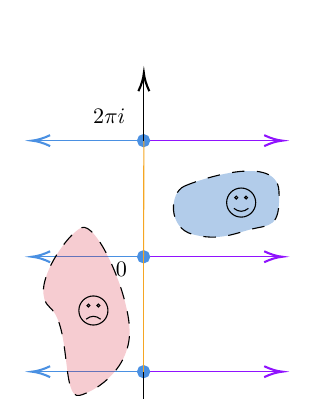
\begin{tikzpicture}[x=0.75pt,y=0.75pt,yscale=-.8,xscale=.8]
    %uncomment if require: \path (0,300); %set diagram left start at 0, and has height of 300
    
    %Straight Lines [id:da22311048865083394] 
    \draw [color={rgb, 255:red, 144; green, 19; blue, 254 }  ,draw opacity=1 ]   (139.98,150.39) -- (221.55,150.39) ;
    \draw [shift={(223.55,150.39)}, rotate = 180] [color={rgb, 255:red, 144; green, 19; blue, 254 }  ,draw opacity=1 ][line width=0.75]    (10.93,-3.29) .. controls (6.95,-1.4) and (3.31,-0.3) .. (0,0) .. controls (3.31,0.3) and (6.95,1.4) .. (10.93,3.29)   ;
    %Straight Lines [id:da18708491874048527] 
    \draw [color={rgb, 255:red, 74; green, 144; blue, 226 }  ,draw opacity=1 ]   (139.98,150.39) -- (74.75,150.39) ;
    \draw [shift={(72.75,150.39)}, rotate = 360] [color={rgb, 255:red, 74; green, 144; blue, 226 }  ,draw opacity=1 ][line width=0.75]    (10.93,-3.29) .. controls (6.95,-1.4) and (3.31,-0.3) .. (0,0) .. controls (3.31,0.3) and (6.95,1.4) .. (10.93,3.29)   ;
    \draw [shift={(139.98,150.39)}, rotate = 180] [color={rgb, 255:red, 74; green, 144; blue, 226 }  ,draw opacity=1 ][fill={rgb, 255:red, 74; green, 144; blue, 226 }  ,fill opacity=1 ][line width=0.75]      (0, 0) circle [x radius= 3.35, y radius= 3.35]   ;
    %Straight Lines [id:da5220594818080124] 
    \draw [color={rgb, 255:red, 144; green, 19; blue, 254 }  ,draw opacity=1 ]   (139.98,219.6) -- (221.55,219.6) ;
    \draw [shift={(223.55,219.6)}, rotate = 180] [color={rgb, 255:red, 144; green, 19; blue, 254 }  ,draw opacity=1 ][line width=0.75]    (10.93,-3.29) .. controls (6.95,-1.4) and (3.31,-0.3) .. (0,0) .. controls (3.31,0.3) and (6.95,1.4) .. (10.93,3.29)   ;
    %Straight Lines [id:da9258702521147173] 
    \draw [color={rgb, 255:red, 74; green, 144; blue, 226 }  ,draw opacity=1 ]   (139.98,219.6) -- (74.75,219.6) ;
    \draw [shift={(72.75,219.6)}, rotate = 360] [color={rgb, 255:red, 74; green, 144; blue, 226 }  ,draw opacity=1 ][line width=0.75]    (10.93,-3.29) .. controls (6.95,-1.4) and (3.31,-0.3) .. (0,0) .. controls (3.31,0.3) and (6.95,1.4) .. (10.93,3.29)   ;
    \draw [shift={(139.98,219.6)}, rotate = 180] [color={rgb, 255:red, 74; green, 144; blue, 226 }  ,draw opacity=1 ][fill={rgb, 255:red, 74; green, 144; blue, 226 }  ,fill opacity=1 ][line width=0.75]      (0, 0) circle [x radius= 3.35, y radius= 3.35]   ;
    %Straight Lines [id:da5593976322909007] 
    \draw [color={rgb, 255:red, 144; green, 19; blue, 254 }  ,draw opacity=1 ]   (140.15,80.46) -- (221.55,80.46) ;
    \draw [shift={(223.55,80.46)}, rotate = 180] [color={rgb, 255:red, 144; green, 19; blue, 254 }  ,draw opacity=1 ][line width=0.75]    (10.93,-3.29) .. controls (6.95,-1.4) and (3.31,-0.3) .. (0,0) .. controls (3.31,0.3) and (6.95,1.4) .. (10.93,3.29)   ;
    %Straight Lines [id:da4484234283967916] 
    \draw [color={rgb, 255:red, 74; green, 144; blue, 226 }  ,draw opacity=1 ]   (139.98,80.46) -- (74.75,80.46) ;
    \draw [shift={(72.75,80.46)}, rotate = 360] [color={rgb, 255:red, 74; green, 144; blue, 226 }  ,draw opacity=1 ][line width=0.75]    (10.93,-3.29) .. controls (6.95,-1.4) and (3.31,-0.3) .. (0,0) .. controls (3.31,0.3) and (6.95,1.4) .. (10.93,3.29)   ;
    \draw [shift={(139.98,80.46)}, rotate = 180] [color={rgb, 255:red, 74; green, 144; blue, 226 }  ,draw opacity=1 ][fill={rgb, 255:red, 74; green, 144; blue, 226 }  ,fill opacity=1 ][line width=0.75]      (0, 0) circle [x radius= 3.35, y radius= 3.35]   ;
    %Straight Lines [id:da7352916869080699] 
    \draw [color={rgb, 255:red, 245; green, 166; blue, 35 }  ,draw opacity=1 ]   (139.98,150.39) -- (140.15,80.46) ;
    %Straight Lines [id:da6707886332001725] 
    \draw [color={rgb, 255:red, 245; green, 166; blue, 35 }  ,draw opacity=1 ]   (139.98,219.6) -- (139.98,150.39) ;
    %Straight Lines [id:da641633314187205] 
    \draw    (140.15,80.46) -- (140.15,41.72) ;
    \draw [shift={(140.15,39.72)}, rotate = 90] [color={rgb, 255:red, 0; green, 0; blue, 0 }  ][line width=0.75]    (10.93,-3.29) .. controls (6.95,-1.4) and (3.31,-0.3) .. (0,0) .. controls (3.31,0.3) and (6.95,1.4) .. (10.93,3.29)   ;
    %Straight Lines [id:da5156062182444048] 
    \draw    (139.98,245.34) -- (139.98,219.6) ;
    %Shape: Polygon Curved [id:ds45793839415006077] 
    \draw  [fill={rgb, 255:red, 0; green, 87; blue, 184 }  ,fill opacity=0.3 ][dash pattern={on 4.5pt off 4.5pt}] (164.51,107.89) .. controls (173.51,103.89) and (220.51,87.89) .. (221.51,110.89) .. controls (222.51,133.89) and (215.51,130.89) .. (204.51,133.89) .. controls (193.51,136.89) and (184.51,140.89) .. (169.51,136.89) .. controls (154.51,132.89) and (155.51,111.89) .. (164.51,107.89) -- cycle ;
    %Shape: Smiley Face [id:dp6908153421809746] 
    \draw   (190,117.75) .. controls (190,112.92) and (193.92,109) .. (198.75,109) .. controls (203.59,109) and (207.51,112.92) .. (207.51,117.75) .. controls (207.51,122.59) and (203.59,126.51) .. (198.75,126.51) .. controls (193.92,126.51) and (190,122.59) .. (190,117.75) -- cycle ; \draw   (194.9,114.78) .. controls (194.9,114.29) and (195.29,113.9) .. (195.78,113.9) .. controls (196.26,113.9) and (196.65,114.29) .. (196.65,114.78) .. controls (196.65,115.26) and (196.26,115.65) .. (195.78,115.65) .. controls (195.29,115.65) and (194.9,115.26) .. (194.9,114.78) -- cycle ; \draw   (200.85,114.78) .. controls (200.85,114.29) and (201.25,113.9) .. (201.73,113.9) .. controls (202.21,113.9) and (202.6,114.29) .. (202.6,114.78) .. controls (202.6,115.26) and (202.21,115.65) .. (201.73,115.65) .. controls (201.25,115.65) and (200.85,115.26) .. (200.85,114.78) -- cycle ; \draw   (194.38,121.25) .. controls (197.29,123.59) and (200.21,123.59) .. (203.13,121.25) ;
    %Shape: Polygon Curved [id:ds49041244870492706] 
    \draw  [fill={rgb, 255:red, 208; green, 2; blue, 27 }  ,fill opacity=0.2 ][dash pattern={on 4.5pt off 4.5pt}] (102.51,132.89) .. controls (111.51,128.89) and (130.51,170.89) .. (131.51,193.89) .. controls (132.51,216.89) and (112.51,230.89) .. (101.51,233.89) .. controls (90.51,236.89) and (96.51,191.89) .. (83.51,180.89) .. controls (70.51,169.89) and (93.51,136.89) .. (102.51,132.89) -- cycle ;
    %Shape: Smiley Face [id:dp8093188113184564] 
    \draw   (101,182.75) .. controls (101,177.92) and (104.92,174) .. (109.75,174) .. controls (114.59,174) and (118.51,177.92) .. (118.51,182.75) .. controls (118.51,187.59) and (114.59,191.51) .. (109.75,191.51) .. controls (104.92,191.51) and (101,187.59) .. (101,182.75) -- cycle ; \draw   (105.9,179.78) .. controls (105.9,179.29) and (106.29,178.9) .. (106.78,178.9) .. controls (107.26,178.9) and (107.65,179.29) .. (107.65,179.78) .. controls (107.65,180.26) and (107.26,180.65) .. (106.78,180.65) .. controls (106.29,180.65) and (105.9,180.26) .. (105.9,179.78) -- cycle ; \draw   (111.85,179.78) .. controls (111.85,179.29) and (112.25,178.9) .. (112.73,178.9) .. controls (113.21,178.9) and (113.6,179.29) .. (113.6,179.78) .. controls (113.6,180.26) and (113.21,180.65) .. (112.73,180.65) .. controls (112.25,180.65) and (111.85,180.26) .. (111.85,179.78) -- cycle ; \draw   (105.38,188) .. controls (108.29,185.67) and (111.21,185.67) .. (114.13,188) ;
    
    % Text Node
    \draw (122,152.4) node [anchor=north west][inner sep=0.75pt]  [xscale=0.8,yscale=0.8]  {$0$};
    % Text Node
    \draw (108.4,60) node [anchor=north west][inner sep=0.75pt]  [xscale=0.8,yscale=0.8]  {$2\pi i$};
    
    
    \end{tikzpicture}
    \]

\noneg \cref{local-injective} does not hold for functions of a real variable (if one interprets
“analytic” as “differentiable”). Using the definition of the derivative, one can show that
$$f(x)=\begin{cases}x+2x^{2}\sin\frac{1}{x}&x\neq0,\\ 0&x=0,\end{cases}$$
satisfies $f^{\prime}(0)=1>0$. One might assume that $f$ is injective in some small neighborhood of $0$. This turns out to be false (see Figure 1). Indeed, the derivative of $f$ is
$$f^{\prime}(x)=\begin{cases}1+4x\sin\frac{1}{x}-2\cos\frac{1}{x}&x\neq0,\\ 1&x=0,\end{cases}$$
which oscillates between arbitrarily large positive and negative values \textit{infinitely often} as $x$ approaches $0$. \sidenote{In complex land, $\sin(1/x)$ has an essential singularity at 0}
Thus, $f$ is neither increasing (nor decreasing) on any open interval containing $0$. In particular, $f$ is not injective on any neighborhood of $0$.
\[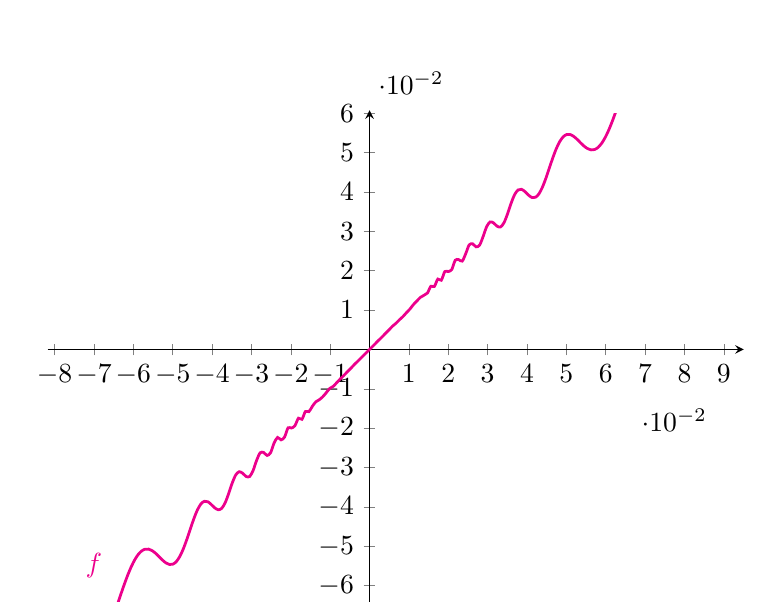
\begin{tikzpicture}[x=0.75pt,y=0.75pt,yscale=1,xscale=1]
    \begin{axis}[
    x=50cm,y=50cm,
    axis lines=middle,
    xmin=-0.08177555075798937,
    xmax=0.09507746322563831,
    ymin=-0.06803825137913687,
    ymax=0.06076043163296842,
    xtick={-0.08,-0.07,...,0.09},
    ytick={-0.06,-0.05,...,0.06},]
    \clip(-0.08,-0.07) rectangle (0.1,0.06);
    \draw[line width=1pt,color=magenta,smooth,samples=200,domain=-0.08177555075798937:0.09507746322563831] plot(\x,{(\x)+2*(\x)^(2)*sin((1/(\x))*180/pi)});
    % \begin{scriptsize}
    \draw[color=magenta] (-0.07,-0.0548509743249033) node {$f$};
    % \end{scriptsize}
    \end{axis}
    \end{tikzpicture}\]

\begin{corollary}
    If $f:\reg\to\C$ is injective, then $f'(z)\neq 0$ on $\reg$.\sidenote{i.e. Conformality}
\end{corollary}
\begin{proof}
    If $f^{\prime}(z_{0})=0$, then $f$ assumes the value $w_{0}=f(z_{0})$ at $z_{0}$ with multiplicity at least two. The local mapping theorem implies $f$ is not injective on any neighborhood of $z_{0}$ since $f$ assumes the value $w_{0}$ at at least two distinct points near $z_{0}$.
\end{proof}

\subsection{Summation via residues}
\eg \label[example]{cotangent-sum} The function $\sin z$ has a simple zero at $z = 0$. \sidenote{$\sin \pi n=0$, and the derivative $\cos z$ always has $\cos \pi n \neq 0$.} Thus, \[\pi\cot\pi z=\frac{\pi\cos\pi z}{\sin\pi z}\]
has a simple pole at each integer. This property makes the cotangent useful for summing
certain infinite series.
Let $p(z)$ be a polynomial with \dashuline{no integer zeros}. Then 
$$f(z)=\frac{\pi\cot\pi z}{p(z)}$$
has an infinite number of simple poles
$$z=0,\pm1,\pm2,\ldots$$
from $\cot\pi z$ and a finite number of poles
$$w_{1},w_{2},\ldots,w_{r},$$
none of which are integers. Let's find $\Res (f;n), n\in \Z$.

\begin{lemma}
    If $g/h$ has a \dashuline{simple pole} at $z_0$ and \dashuline{$g(z_0) \neq 0$}, then $$\Res \left(\frac{g(z)}{h(z)};z_{0}\right)=\frac{g(z_{0})}{h^{\prime}(z_{0})}$$
\end{lemma}
\begin{proof}
    Since $z_{0}$ is a simple pole of $g/h$, it is a simple zero of $h$ and $h^{\prime}(z_{0})\neq0$. Thus,
    \begin{align*}
        \operatorname{Res}\left(\frac{g(z)}{h(z)};z_{0}\right)&=\lim_{z\to z_{0}}(z-z_{0})\frac{g(z)}{h(z)}\\
        &=\lim_{z\to z_{0}}g(z)\frac{z-z_{0}}{h(z)-h(z_{0})}\\
        &=g(z_{0})\lim_{z\to z_{0}}\frac{z-z_{0}}{h(z)-h(z_{0})}\\
        &=\frac{g(z_{0})}{h^{\prime}(z_{0})}
    \end{align*}

\end{proof}

Returning to \cref{cotangent-sum}: For each $n\in\mathbb{Z}$, the function $f(z)$ has residues
\[\text{Res}(f;n)=\text{Res}\left(\frac{\frac{\pi\cos\pi z}{p(z)}}{\sin\pi z};n\right)=\frac{\frac{\pi\cos n\pi}{p(n)}}{\pi\cos n\pi}=\frac{1}{p(n)}\]
Let $\gamma_N$ be the rectangular curve with vertices $\pm (N+\rt{\frac{1}{2}})\pm iN$\sidenote{we really want to avoid integers because they are poles of $f$}, where $N\in \N$ is so large that all of $p(z)$'s zeros $w_1,\dots,w_r$ are inside $\gamma_N$. 
\[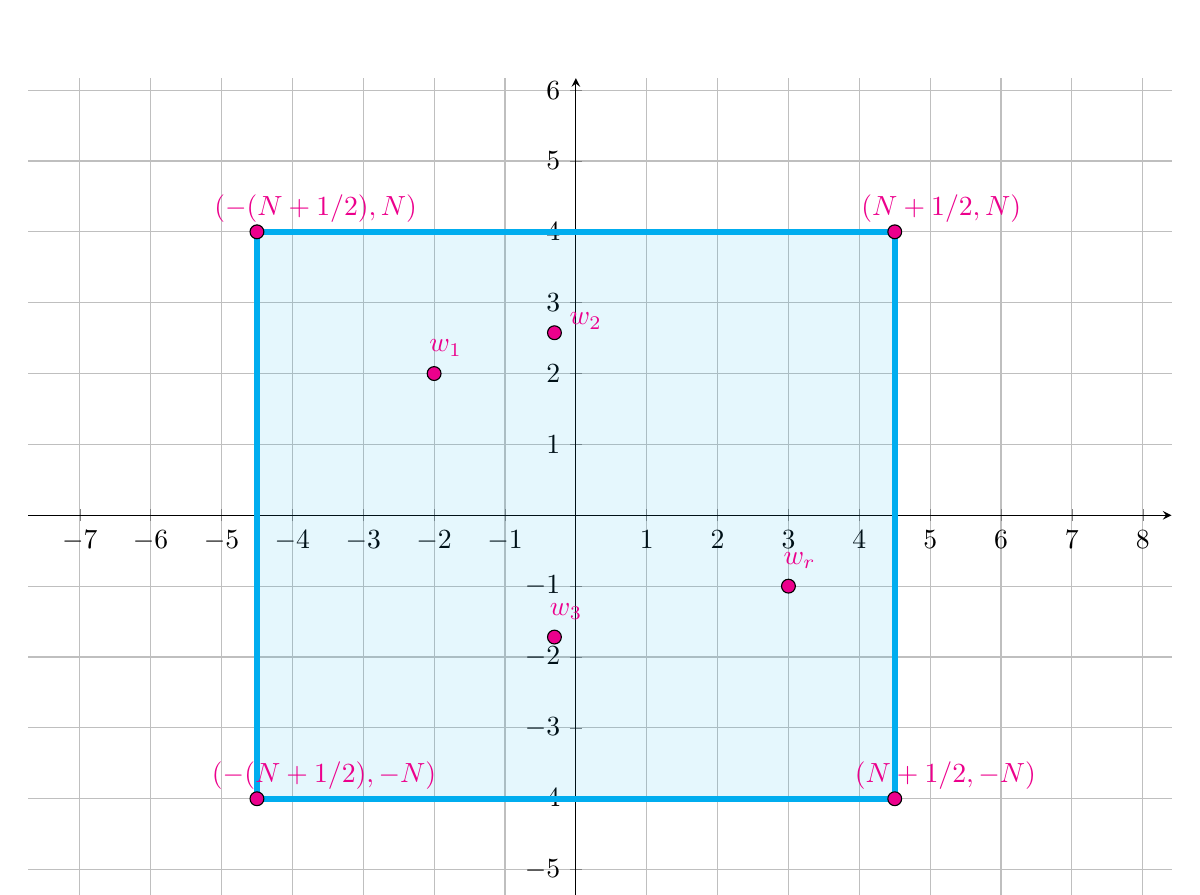
\begin{tikzpicture}[x=.75pt,y=.75pt]
    \begin{axis}[
    x=.9cm,y=.9cm,
    axis lines=middle,
    ymajorgrids=true,
    xmajorgrids=true,
    xmin=-7.727512941297836,
    xmax=8.405996615862398,
    ymin=-5.580265586094737,
    ymax=6.169462261448943,
    xtick={-7,-6,...,8},
    ]
    \clip(-7.727512941297836,-5.580265586094737) rectangle (8.405996615862398,6.169462261448943);
    \fill[line width=2pt,color=cyan,fill=cyan,fill opacity=0.1] (-4.5,4) -- (-4.5,-4) -- (4.5,-4) -- (4.5,4) -- cycle;
    \draw [line width=2pt,color=cyan] (-4.5,4)-- (-4.5,-4);
    \draw [line width=2pt,color=cyan] (-4.5,-4)-- (4.5,-4);
    \draw [line width=2pt,color=cyan] (4.5,-4)-- (4.5,4);
    \draw [line width=2pt,color=cyan] (4.5,4)-- (-4.5,4);
    \begin{scriptsize}
    \draw [fill=magenta] (-4.5,4) circle (2.5pt);
    \draw[color=magenta] (-3.671769318795448,4.32797572696716) node {$(-(N+1/2), N)$};
    \draw [fill=magenta] (-4.5,-4) circle (2.5pt);
    \draw[color=magenta] (-3.552482741663025,-3.679135763046743) node {$(-(N+1/2), -N)$};
    \draw [fill=magenta] (4.5,-4) circle (2.5pt);
    \draw[color=magenta] (5.215080677570078,-3.679135763046743) node {$(N+1/2, -N)$};
    \draw [fill=magenta] (4.5,4) circle (2.5pt);
    \draw[color=magenta] (5.1554373890038665,4.32797572696716) node {$(N+1/2, N)$};
    \draw [fill=magenta] (-2,2) circle (2.5pt);
    \draw[color=magenta] (-1.8377381953844423,2.3597472042821788) node {$w_1$};
    \draw [fill=magenta] (-0.30192351480449386,2.5759541253346954) circle (2.5pt);
    \draw[color=magenta] (0.137904471247412,2.7412692678027414) node {$w_2$};
    \draw [fill=magenta] (-0.30192351480449386,-1.7183626514325379) circle (2.5pt);
    \draw[color=magenta] (-0.137904471247412,-1.3530475089644918) node {$w_3$};
    \draw [fill=magenta] (3,-1) circle (2.5pt);
    \draw[color=magenta] (3.157387222035778,-0.6373280461699531) node {$w_r$};
    \end{scriptsize}
    \end{axis}
    \end{tikzpicture}\]
By the residue theorem,\hypertarget{cotangent-integral}{}
\begin{align*}
    {\frac{1}{2\pi i}}\int_{\gamma_{N}}{\frac{\pi\cot\pi z}{p(z)}}\d z&=\sum_{n=-N}^{N}\Res \left({\frac{\pi\cot\pi z}{p(z)}};n\right)+\sum_{j=1}^{r}\Res \left({\frac{\pi\cot\pi z}{p(z)}};w_{j}\right)\\
    &= \sum_{n=-N}^{N}\Res \left({\frac{\pi\cos\pi z/p(z)}{\sin \pi z}};n\right)+\sum_{j=1}^{r}\Res \left({\frac{\pi\cot\pi z}{p(z)}};w_{j}\right)\\
    &= \sum_{n=-N}^{N}\frac{1}{p(n)}+\sum_{j=1}^{r}\Res \left(\frac{\pi\cot \pi z}{p(z)}; w_j\right)
\end{align*}
\textit{Claim}: the integral tends to 0 as $N\to \infty$ if $\deg p\geq 2$. \hypertarget{integral-of-1-over-pn}{Hence}, \[\sum_{n=-\infty}^{\infty}{\frac{1}{p(n)}}=-\sum_{j=1}^{r}\mathrm{Res}\left({\frac{\pi\cot\pi z}{p(z)}};w_{j}\right)\]
Observe that $\deg p(z)\geq2$ implies that $\sum_{n=0}^\infty\frac{1}{p(n)}$ and $\sum_{n=-\infty}^{-1}\frac{1}{p(n)}$ converge by the comparison test with just the leading term.

\begin{lemma}
    There is an $M > 0$ such that $|\cot \pi z|\leq M$ on $\gamma_N$ for all $N\in \N$. 
\end{lemma}
\begin{proof}
    If $z=x+iy$, in which $x,y\in\mathbb{R}$, then
\[|\cot\pi z|=\left|\frac{e^{i\pi x}+e^{-i\pi z}}{e^{i\pi x}-e^{-i\pi x}}\right|=\left|\frac{1+e^{-2\pi ix}}{1-e^{-2\pi ix}}\right|=\left|\frac{1+e^{-2\pi ix}e^{2\pi y}}{1-e^{-2\pi ix}e^{2\pi y}}\right|\]
On the \textbf{vertical} sides of $\gamma_{N}$, we have $z=\pm(N+\frac{1}{2})+iy$ where $-N\leq y\leq N$ so that
\[|\cot\pi z|=\left|\frac{1+e^{\mp2\pi i(N+\frac{1}{2})}e^{2\pi y}}{1-e^{\mp2\pi i(N+\frac{1}{2})}e^{2\pi y}}\right|=\left|\frac{1-e^{2\pi y}}{1+e^{2\pi y}}\right|\]
This tends to $1$ independently of $N$ as $y\to+\infty$. Thus, there is an $M_1$ such that $|\cot \pi z|\leq M_1$ on the \textbf{vertical} sides of each $\gamma_{N}$.
On the \textbf{horizontal} sides of $\gamma_{N}$, we have $z=x\pm iN$ where $-(N+\frac{1}{2})\leq x\leq(N+\frac{1}{2})$.
Thus,
$$|\cot\pi z|=\left|\frac{1+e^{-2\pi is}e^{\pm2\pi N}}{1-e^{-2\pi is}e^{\pm2\pi N}}\right|\leq\frac{e^{\pm2\pi N}+1}{|e^{\pm2\pi N}-1|}$$
which tends to $1$ as $N\to\infty$. Consequently, there is an $M_{2}$ such that $|\cot\pi z|\leq M_{2}$ on the vertical sides of each $\gamma_{N}$.
Set $M=\max\{M_{1},M_{2}\}$ and conclude that
\[|\cot\pi z|\leq M\]
on each $\gamma_{N}$ for $N\in\mathbb{N}$.
\end{proof}

Since $\deg p(z)\geq2$, there exists a constant $C$ such that
$$\left|\frac{1}{p(z)}\right|\leq\frac{C}{|z|^{2}}$$
for sufficiently large $|z|$. Thus, for sufficiently large $N$,
$$\left|\frac{1}{2\pi i}\int_{\gamma}\frac{\pi\cot\pi z}{p(z)}\ \d z\right|\leq M\cdot\frac{C}{N^{2}}\cdot\underbrace{(2N+2(N+1))}_{\text{periment of $\gamma_{\infty}$}}\leq\frac{5MC}{N},$$
which tends to zero as $N\to\infty$. Consequently, the integral ${\frac{1}{2\pi i}}\int_{\gamma_{N}}{\frac{\pi\cot\pi z}{p(z)}}\d z$ \hyperlink{cotangent-integral}{here} tends to zero as $N\to\infty$. This yields \hyperlink{integral-of-1-over-pn}{this result}:\[\sum_{n=-\infty}^{\infty}{\frac{1}{p(n)}}=-\sum_{j=1}^{r}\mathrm{Res}\left({\frac{\pi\cot\pi z}{p(z)}};w_{j}\right)\]

\eg Consider the sum \[\sum_{n=-\infty}^{\infty}\frac{1}{n^2+a^2} = \sum_{n=0}^{\infty}\frac{1}{n^2+a^2}+\sum_{n=1}^{\infty}\frac{1}{(-n)^2+a^2}= \frac{1}{a^2} +2\sum_{n=1}^{\infty}\frac{1}{\rt{n^2+a^2}}\] when $a\neq 0$.

Set $p(z)= z^2+a^2$ which has zeros $w_1=ia, w_2=-ia$. \hyperlink{integral-of-1-over-pn}{This result} implies 
\[\sum_{n=-\infty}^{\infty}{\frac{1}{n^{2}+a^{2}}}=-\left[\mathrm{Res}\left({\frac{\pi\cot\pi z}{z^{2}+a^{2}}};i a\right)+\mathrm{Res}\left({\frac{\pi\cot\pi z}{z^{2}+a^{2}}};-i a\right)\right]
\]
we compute the two residues required:
\begin{align*}
    \mathrm{Res}\left(\frac{\pi\cot\pi z}{z^{2}+a^{2}};ia\right)&=\operatorname*{lim}_{z\to ia}\left(z-ia\right)\cdot\frac{\pi\cot\pi z}{z^{2}+a^{2}}\\
    &=\operatorname*{lim}_{z\to ia}\left(z-ia\right)\cdot\frac{\pi\cot\pi z}{(z-ia)(z+ia)}\\
    &=\operatorname*{lim}_{z\to ia}\frac{\pi\cot\pi z}{z+ia}\\ &=\frac{\pi\cot\pi ia}{2ia}
\end{align*}
and \begin{align*}
    \mathrm{Res}\left({\frac{\pi\cot\pi z}{z^{2}+a^{2}}};-i a\right)&=\operatorname*{lim}_{z\to-i a}(z-(-i a))\cdot{\frac{\pi\cot\pi z}{z^{2}+a^{2}}}\\
    &=\operatorname*{lim}_{z\to-i a}(z+i a)\cdot{\frac{\pi\cot\pi z}{(z-i a)(z+i a)}}\\
    &=\operatorname*{lim}_{z\to-i a}{\frac{\pi\cot\pi z}{z-i a}}\\
    &={\frac{\pi\cot\pi(-i a)}{-2i a}}\\
    &={\frac{\pi\cot\pi i a}{2i a}}
\end{align*}
Putting this together we obtain \begin{align*}
    \sum_{n=-\infty}^{\infty}{\frac{1}{n^{2}+a^{2}}}&=-\left[\mathrm{Res}\left({\frac{\pi\cot\pi z}{z^{2}+a^{2}}};i a\right)+\mathrm{Res}\left({\frac{\pi\cot\pi z}{z^{2}+a^{2}}};-i a\right)\right]\\
    &= -\left(\frac{\pi\cot\pi i a}{2i a}+\frac{\pi\cot\pi i a}{2i a}\right)\\
    &=-\frac{\pi\cot\pi i a}{i a}\\
    &=-\frac{\pi}{i a}\cdot\frac{\cos\pi i a}{\sin\pi i a}\\
    &=-\frac{\pi}{i a}\cdot\frac{e^{i(\pi i a)}+e^{-i(\pi i a)}}{2}\cdot\frac{2i}{e^{i(\pi i a)}-e^{-i(\pi i a)}}\\
    &=-\frac{\pi}{a}\cdot\frac{e^{-\pi a}+e^{\pi a}}{e^{-\pi a}-e^{\pi a}}\\
    &=\frac{\pi}{a}\cdot\frac{e^{\pi a}+e^{-\pi a}}{e^{\pi a}-e^{-\pi a}}\\
    &=\frac{\pi\coth\pi a}{a}
\end{align*}

Write $$\sum_{n=-\infty}^\infty\frac{1}{n^2+a^2}=\frac{1}{a^2}+2\sum_{n=1}^\infty\frac{1}{n^2+a^2}$$ and observe that $$\frac{1}{a^2}+2\sum_{n=1}^\infty\frac{1}{n^2+a^2}=\frac{\pi\coth\pi a}{a}$$ and hence $$\sum_{n=1}^\infty\frac{1}{n^2+a^2}=\frac{\pi a\coth\pi a-1}{2a^2}$$

We observe that this is actually \textbf{analytic}
of $a$ on a punctured neighborhood of 0. In fact, we can even show that $a=0$ is a \textbf{removable singularity}.\sidenote{plug in $a=0$, observe that the function is bounded!}

Using the Laurent series:
$$\coth z=\frac{1}{z}+\frac{z}{3}-\frac{z^{3}}{45}+\frac{2z^{5}}{945}+\cdots$$
we have
\begin{align*}
    \frac{\pi a\coth\pi a-1}{2a^{2}}&=\frac{\pi a\left(\frac{1}{\pi a}+\frac{\pi a}{3}-\frac{(\pi a)^{3}}{45}+\cdots\right)-1}{2a^{2}}\\
    &=\frac{\left(1+\frac{\pi^{2}a^{2}}{3}-\frac{\pi^{4}a^{4}}{45}+\cdots\right)-1}{2a^{2}}\\
&=\frac{\frac{\pi^{2}a^{2}}{3}-\frac{\pi^{4}a^{4}}{45}+\cdots}{2a^{2}}\\
&=\frac{\pi^{2}}{6}-\frac{\pi^{4}a^{2}}{90}+\cdots
\end{align*}
Thus, $a=0$ is a removable singularity and it yields Euler's celebrated formula:
\[\sum_{n=1}^{\infty}\frac{1}{n^2}= \frac{\pi^2}{6}\]

\section{Prime Number Theorem}
\subsection{Newman's Tauberian theorem}
A ``Tauberian theorem'' is a result in which a strong convergence result is deduced from a weaker convergence result and an additional hypothesis. G.H. Hardy and J.E. Littlewood, who coined the term in honor of A. Tauber. 

The following is a Tauberian theorem of D.J. Newman, deduced in 1980.
\begin{theorem}[Newman's]\label[theorem]{newmans-tauberian}
    Let $f:[0,\infty)\to \C$ be \textbf{bounded} and \textbf{piecewise continuous}\sidenote{piecewise cont. means that it has finite amount of discontinuities on any finite intervals}.
For $\re z > 0$, let the \textbf{Laplace transfomation} of $f$ be
\begin{equation*}
g(z) = \int_0^{\infty} f(t) e^{-zt}\d t.
\end{equation*}
Suppose $g$ has an \textbf{analytic continuation} to a neighborhood of $\re z \geq 0$\sidenote{this is the \textbf{closed} half plane: plugging in 0 is fine}. Then 
\begin{equation*}
g(0) = \lim_{T\to\infty} \int_0^T f(t)\d t.
\end{equation*}
In particular, $\displaystyle\int_0^{\infty} f(t)\d t$ converges.\sidenote{Note this is not obvious: if $f$ is the constant function of 1, $g$ has a pole at 0 and so the hyp. is not satisfied. The integral $\int_{0}^{\infty}1\d t$ diverges!}
\end{theorem}
\begin{proof}[Proof (behold, this one is long!)]
    Note that $g(z)$ is analytic on $\re z > 0$ (Exercise 6, HW9).
    
    \spl
    \begin{lemma}\label[lemma]{gt-entire}
        Let $f:[0,\infty)\to\mathbb{C}$ be piecewise continuous. For each $T>0$, the function\sidenote{a truncated Laplace; can also be proven with technique on Ex6 HW9.} \begin{equation}\label{nt-eq2}
            g_{T}(z)=\int_{0}^{T}e^{-zt}f(t)\d t
        \end{equation} is entire.
    \end{lemma}
    \begin{proof}
        Fix $T>0$ and let
$$M=\sup_{0\leq t\leq T}|f(t)|,$$
which is finite since $[0,T]$ is compact and $f$ is piecewise continuous.\sidenote{Recall that a piecewise continuous function has only
finitely many discontinuities, all of which are jump
discontinuities.} Then,
$$c_{n}=\int_{0}^{T}f(t)t^{n}\,dt\quad\text{satisfies}\quad|c_{n}|\leq\frac{MT^{n+1}}{n+1}$$
Since $e^{z}$ is entire, its power series representation converges uniformly on $[0,T]$. Thus,
$$g_{T}(z)=\int_{0}^{T}f(t)e^{-zt}\d t=\int_{0}^{T}f(t)\left(\sum_{n=0}^{\infty}\frac{(-zt)^{n}}{n!}\right)\d t$$ $$=\sum_{n=0}^{\infty}\frac{(-1)^{n}z^{n}}{n!}\int_{0}^{T}f(t)t^{n}\d t=\sum_{n=0}^{\infty}\frac{(-1)^{n}c_{n}}{n!}z^{n}$$
defines an entire function since its radius of convergence is the reciprocal of
$$\limsup_{n\to\infty}\left|\frac{(-1)^{n}c_{n}}{n!}\right|^{\frac{1}{n}}\leq\limsup_{n\to\infty}\frac{M^{\frac{1}{n}}T^{\frac{n+1}{n}}}{(n+1)^{\frac{1}{n}}(n!)^{\frac{1}{n}}}=\frac{1\cdot T}{1\cdot\infty}=0$$\sidenote{recall $n^{1/n}=1$ and $(n!)^{1/n}\to \infty$}
by the \hyperlink{cauchy-hadamard}{Cauchy-Hadamard formula}.
    \end{proof}
    \spl

    Now we must show \begin{equation}\label{nt-eq3}
        \operatorname*{lim}_{T\rightarrow\infty}g_{T}(0)=g(0)
    \end{equation}
\begin{enumerate}[align=left, label=\textit{Step \arabic*:}]
    \item Let $\|f\|_{\infty}=\sup_{t\geq0}|f(t)|$, which is finite by assumption. For $\re z>0$,\sidenote{We look at the tail of the integral}
    \begin{equation}\label{nt-eq4}
        \begin{aligned}
            |g(z)-g_{T}(z)|&=\left|\int_{0}^{\infty}e^{-zt}f(t)\,dt-\int_{0}^{T}e^{-zt}f(t)\,dt\right|\\
        &=\left|\int_{T}^{\infty}e^{-zt}f(t)\,dt\right|\\
        &\leq\int_{T}^{\infty}e^{-\re (zt)}|f(t)|\,dt\\
        &\leq\|f\|_{\infty}\int_{T}^{\infty}e^{-t\re z}\d t\\
        &=\|f\|_{\infty}\,\frac{e^{-T\re z}}{\re z}
        \end{aligned}
    \end{equation}

    \item For $\re z<0$\sidenote{because $g$ has analytic continuation to an open nbd of any $\re z \geq 0$}, \begin{equation}\label{nt-eq5}
        \begin{aligned}
            |g_{T}(z)|&=\left|\int_{0}^{T}e^{-zt}f(t)\,dt\right|\leq\int_{0}^{T}e^{-\re (zt)}|f(t)|\,dt\\
            &\leq\|f\|_{\infty}\int_{0}^{T}e^{-t\re z}\,dt\\
            &\leq\|f\|_{\infty}\int_{-\infty}^{T}e^{-t\re z}\,dt\\
            &=\|f\|_{\infty}\,\frac{\gt{e^{-T\re z}}}{|\re z|}
        \end{aligned}
    \end{equation}
    
    \item Suppose that $g$ has an analytic continuation to an open region $\Omega$ that contains the closed half plane $\re z\geq0$. Let $R>0$ and let $\delta_{R}>0$ be small enough to ensure that $g$ is analytic on an open region that contains the curve $C_{R}$ (and its interior) formed by intersecting the circle $|z|=R$ with the vertical line $\re z=-\delta_{R}$.\sidenote{The imaginary line segment $[-iR,iR]$ is \textbf{compact} and can be
    covered by \textbf{finitely} many open disks (yellow) upon which $g$ is analytic. Thus, there is a
    $\delta_R>0$ such that g is analytic on an open region that contains the curve $C_R$.}\drawing{0.5\linewidth}{image-10.png}

    \item For each $R>0$, Cauchy's integral formula implies \sidenote{\rt{this part} evals to 1 when $z=0$, so they disappear and the rest is from CIF. \textit{This is the clever bit!}}\begin{equation}\label{nt-eq6}
        g_{T}(0)-g(0)={\frac{1}{2\pi i}}\int_{C_{R}}\left(g_{T}(z)-g(z)\right)\rt{e^{z T}\left(1+{\frac{z^{2}}{R^{2}}}\right)}{\frac{\d z}{z}}
    \end{equation}
    We examine the contributions to this integral over the two curves
    $$C_{R}^{+}=C_{R}\cap\{z:\mathrm{Re}\,z\geq0\}\qquad\text{and}\qquad C_{R}^{-}=C_{R}\cap\{z:\mathrm{Re}\,z\leq0\}.$$

    \item We first examine the contribution of $C_{R}^{+}$ in \cref{nt-eq6}. Let $z=Re^{it}$: \begin{equation}\label{nt-eq7}
        \begin{aligned}
            \left|{\frac{1}{z}}\left(1+{\frac{z^{2}}{R^{2}}}\right)\right|&=\left|{\frac{1}{z}}+{\frac{z}{R^{2}}}\right|=\left|{\frac{1}{R e^{i t}}}+{\frac{R e^{i t}}{R^{2}}}\right|\\ 
            &={\frac{1}{R^{2}}}|R e^{-i t}+R e^{i t}|={\frac{1}{R^{2}}}|\bar{z}+z|\\ 
            &={\frac{2|\re z|}{R^{2}}}
        \end{aligned}
    \end{equation}
    For $z\in \C$: \begin{equation}\label{nt-eq8}
        |e^{z T}|= e^{T\,\mathrm{Re}\,z}
    \end{equation}
    and hence \cref{nt-eq4,nt-eq7,nt-eq8} imply: 
    \begin{equation}\label{nt-eq9}
        \begin{aligned}
           &\left|\frac{1}{2\pi i}\int_{C_{R}^{+}}\left(g_{T}(z)-g(z)\right)e^{z T}\left(1+\frac{z^{2}}{R^{2}}\right)\frac{d z}{z}\right|\\
    \leq&\frac{1}{2\pi}\underbrace{\left(\|f\|_{\infty}\,\frac{e^{-T\re z}}{\re z}\right)}_{\text{by \ref{nt-eq4}}}\underbrace{(e^{T\re z})}_{by \ref{nt-eq8}}\underbrace{\left(\frac{2 |\re z|}{R^{2}}\right)}_{\text{by \ref{nt-eq7}}}(\pi R)\\
    =&\frac{\|f\|_{\infty}}{R} 
        \end{aligned}
    \end{equation}

   
    \item[\textit{Step 6a:}] We examine the contribution of $C_R^-$ in \cref{nt-eq6} in 6a and 6b. Since
    the integrand in the following integral is \textbf{analytic}\sidenote{see \cref{gt-entire}} in $\re z<0$, we can replace the contour\sidenote{by Cauchy's deformation} $C_R^-$ with the left-hand side of the circle $|z|=R$ in the
    computation
    \begin{equation}
        \left|\frac{1}{2\pi i} \int_{C_{R}^{-}}g_{T}(z)e^{z T}\left(1+\frac{z^{2}}{R^{2}}\right)\frac{d z}{z}\right|
    \end{equation}
    \begin{equation}\label{nt-eq11}
        \begin{aligned}
            &=\left|\frac{1}{2\pi i}\int_{|z|=R}g_{T}(z)e^{z T}\left(1+\frac{z^{2}}{R^{2}}\right)\frac{d z}{z}\right|\\
            &\leq \frac{1}{\mathbf{2}\gt{\pi}}
            \underbrace{\left(\left\|f\right\|_{\infty}\frac{\bt{e^{-T\re z}}}{\rt{\left|\re z\right|}}\right)}_{\text{by (\ref{nt-eq5})}}(\bt{e^{T\re z}})
            \underbrace{\left(\frac{\mathbf{2}\rt{\left|\re z\right|}}{R^{2}}\right)}_{\text{by (\ref{nt-eq7})}}(\gt{\pi} R)\\
            &=\frac{\left\|f\right\|_{\infty}}{R}
        \end{aligned}
    \end{equation}
    \sidenote{The integrand in \cref{nt-eq11} is analytic in $\re  z<0$. Cauchy's theorem ensures that the integral over $C_R^{-}$ equals the integral over the semicircle $\{z:|z|=R, \re  z \leq 0\}$.}\drawing{0.5\linewidth}{image-15.png}
    
    \item[\textit{Step 6b:}] Next we focus on the corresponding integral with $g$ in place of $g_T$. Let
    $$
    M=\sup _{z \in C_R^{-}}|g(z)|,
    $$
    which is finite since $C_R^{-}$is compact. Since $|z| \geq \delta_R$ for $z \in C_R^{-}$,
    $$
    \left|g(z) e^{z T}\underbrace{\rt{\left(1+\frac{z^2}{R^2}\right)}}_{\leq 2} \frac{1}{z}\right| \leq \frac{2 M e^{T \re  z}}{\delta_R} .
    $$
    
    Fix $\epsilon>0$ and obtain a curve $C_R^{-}(\epsilon)$ by removing, from the beginning and end of $C_R^{-}$, \textcolor{purple}{two arcs each of length $\epsilon \delta_R /(4 M)$}. 
    \drawing{0.5\linewidth}{image-16.png}
    Then there is a $\rho>0$ such that $\re  z<-\rho$ for each $z \in C_R^{-}(\epsilon)$.
    % \drawing{0.5\linewidth}{image-18.png}
    Consequently,\sidenote{$\delta_R<R$ so we are bounding above by making the denom. smaller}
    $$
    \begin{aligned}
    \limsup _{T \rightarrow \infty}\left|\int_{C_R^{-}} \gt{g(z)} \bt{e^{z T}}\left(\rt{1+\frac{z^2}{R^2}}\right) \frac{d z}{z}\right| & 
    \leq \limsup _{T \rightarrow \infty}
    \Bigg(\underbrace{\textcolor{blue}{\frac{2 M e^{-\rho T}}{\delta_R} \cdot \pi R}}_{\text {from } C_R^{-}(\epsilon)}
    +\underbrace{\frac{\rt{2}\cdot \bt{1}
    \cdot \gt{M}}{\delta_R} 
    \cdot 2\textcolor{purple}{\frac{ \epsilon \delta_R}{4 M}}}_{\text {from the two arcs}}\Bigg) \\
    & =\epsilon 
    \end{aligned}
    $$
    Since $\epsilon>0$ was arbitrary,\sidenote{we couldn't omit the $\epsilon$ in prev. steps because the two arcs were indep. of $T$ and hence can't get cancelled by having $T\to \infty$.}
    \begin{equation}\label{nt-eq12}
        \limsup _{T \rightarrow \infty}\left|\int_{C_R^{-}} g(z) e^{z T}\left(1+\frac{z^2}{R^2}\right) \frac{d z}{z}\right|=0
    \end{equation}
    \setcounter{enumi}{6}

    \item For each fixed $R$,
    \begin{align*}
        &\limsup_{T\to0}|g_{T}(0)-g(0)|\\
        =&\limsup_{T\to0}\left|\frac{1}{2\pi i}\int_{C_{R}}\left(g_{T}(z)-g(z)\right)e^{zT}\left(1+\frac{z^{2}}{R^{2}}\right)\frac{\d z}{z}\right| &&\text{by (\ref{nt-eq6})}\\
        \leq &\underbrace{\left\|f\right\|_{R}}_{\text{from }C_{R}^{+}}+\underbrace{\left(\left\|f\right\|_{\infty}+0\right)}_{\text{from }C_{R}^{-}} &&\text{by \labelcref{nt-eq9,nt-eq11,nt-eq12}}\\
        =& \frac{2\,||f||_\infty}{R}
    \end{align*} 

Since $R > 0$ was arbitrary, it follows that we can let $R\to \infty$ and get \[\operatorname*{limsup}_{T\rightarrow0}|g_{T}({0}){-}g({0})|{=}{0}\]
\end{enumerate}
Hence, $\operatorname*{lim}_{T\to\infty}g_{T}(0)=g(0)$.\sidenote{Tail is 0 so we are good}
\end{proof}

\subsection{Summary of proof of PNT}
\begin{theorem}[Prime Number]
    Let $\pi(x)$ be the number of primes $\leq x$ for some $x\in \R_{\geq 0}$.\sidenote{For instance, $\pi(10.5) = 4$ since $2,3,5,7\leq 10.5$.} Then \[\lim_{x\to \infty}\frac{\pi(x)}{x/\ln x}=1\]
\end{theorem}
\begin{figure}[htbp]
    \centering
    % This file was created with tikzplotlib v0.10.1.
% \begin{tikzpicture}
\begin{tikzpicture}%[x=0.75pt,y=0.75pt,yscale=1.1,xscale=1.1]

% \definecolor{black}{RGB}{176,176,176}
% \definecolor{magenta}{RGB}{255,127,14}
% \definecolor{cyan}{RGB}{31,119,180}

\begin{axis}[
tick align=outside,
tick pos=left,
x grid style={black},
xlabel={\(\displaystyle x \leq 100\)},
xmin=-5.04, xmax=105.84,
xtick style={color=black},
y grid style={black},
ylabel={$\rt{\frac{x}{\ln x}}$ and $\bt{\pi(x)}$},
ymin=-1.39490921850156, ymax=29.2930935885328,
ytick style={color=black}
]
\addplot [thick, cyan, const plot mark left]
table {%
0 0
2 1
3 2
5 3
7 4
11 5
13 6
17 7
19 8
23 9
29 10
31 11
37 12
41 13
43 14
47 15
53 16
59 17
61 18
67 19
71 20
73 21
79 22
83 23
89 24
97 25
};
\addplot [thick, magenta]
table {%
4 10.3547977982484
4.2 9.65329667196755
4.4 9.13612648160719
4.6 8.7443111496587
4.8 8.44155052431592
5 8.20428118761098
5.2 8.01654336330027
5.4 7.86714486074388
5.6 7.74800608869024
5.8 7.65314957549306
6 7.57805903584563
6.2 7.5192593817862
6.4 7.47403365651635
6.6 7.44022750321727
6.8 7.41611114139458
7 7.40028004455914
7.2 7.39158222740837
7.4 7.38906418345587
7.6 7.39193012293241
7.8 7.39951084551978
8 7.41123969302713
8.2 7.42663377297653
8.4 7.44527915360876
8.6 7.46681908441012
8.8 7.49094454518631
9 7.51738660429497
9.2 7.54591019490969
9.40000000000001 7.57630901188945
9.6 7.60840130101444
9.8 7.64202636394601
10 7.6770416411066
10.2 7.71332026416685
10.4 7.75074899240532
10.6 7.78922646462551
10.8 7.82866171185321
11 7.86897288663098
11.2 7.91008617307111
11.4 7.95193484844151
11.6 7.99445847233134
11.8 8.03760218366919
12 8.08131608927284
12.2 8.12555473036858
12.4 8.17027661576329
12.6 8.21544381218863
12.8 8.26102158384465
13 8.30697807441319
13.2 8.35328402584184
13.4 8.39991252905441
13.6 8.44683880245882
13.8 8.49403999472043
14 8.54149500877207
14.2 8.58918434445481
14.4 8.63708995754214
14.6 8.6851951332037
14.8 8.73348437222317
15 8.78194328850549
15.2 8.83055851659701
15.4 8.87931762810392
15.6 8.92820905603361
15.8 8.97722202620314
16 9.02634649496301
16.2 9.0755730925738
16.4 9.12489307165138
16.6 9.17429826016389
16.8 9.22378101852308
17 9.27333420036391
17.2 9.32295111665152
17.4 9.37262550279436
17.6 9.42235148847709
17.8 9.47212356995722
18 9.52193658459677
18.2 9.5717856874239
18.4 9.62166632954052
18.6 9.67157423821073
18.8 9.72150539848136
19 9.77145603620079
19.2 9.82142260231508
19.4 9.8714017583326
19.6 9.92139036285822
19.8 9.97138545910797
20 10.0213842633231
20.2 10.0713841540101
20.4 10.1213826619401
20.6 10.1713774608464
20.8 10.221366358766
21 10.2713472899733
21.2 10.3213183074613
21.4 10.3712775759278
21.6 10.4212233652277
21.8 10.4711540442578
22 10.5210680752401
22.2 10.5709640083761
22.4 10.6208404768429
22.6 10.6706961921086
22.8 10.7205299395421
23 10.7703405742978
23.2 10.8201270174553
23.4 10.8698882523958
23.6 10.9196233214005
23.8 10.9693313224532
24 11.019011406236
24.2 11.0686627733029
24.4 11.1182846714206
24.6 11.1678763930656
24.8 11.2174372730655
25 11.2669666863782
25.2 11.3164640459969
25.4 11.365928800975
25.6 11.4153604345624
25.8 11.4647584624463
26 11.5141224310901
26.2 11.5634519161636
26.4 11.6127465210605
26.6 11.6620058754959
26.8 11.7112296341799
27 11.7604174755634
27.2 11.8095691006503
27.4 11.858684231873
27.6 11.9077626120276
27.8 11.9568040032649
28 12.005808186134
28.2 12.0547749586758
28.4 12.1037041355631
28.6 12.1525955472848
28.8 12.2014490393721
29 12.2502644716633
29.2 12.2990417176066
29.4 12.347780663597
29.6 12.3964812083469
29.8 12.445143262288
30 12.4937667470025
30.2 12.542351594682
30.4 12.5908977476139
30.6 12.6394051576919
30.8 12.6878737859501
31 12.7363036021208
31.2 12.7846945842121
31.4 12.8330467181066
31.6 12.8813599971791
31.8 12.9296344219319
32 12.9778699996482
32.2 13.0260667440607
32.4 13.074224675037
32.6 13.1223438182784
32.8 13.1704242050338
33 13.2184658718259
33.2 13.266468860191
33.4 13.3144332164298
33.6 13.3623589913702
33.8 13.4102462401408
34 13.4580950219549
34.2 13.5059053999036
34.4 13.5536774407595
34.6 13.6014112147877
34.8 13.6491067955668
35 13.6967642598167
35.2 13.7443836872349
35.4 13.79196516034
35.6 13.8395087643216
35.8 13.8870145868975
36 13.9344827181771
36.2 13.9819132505305
36.4 14.0293062784635
36.6 14.0766618984986
36.8 14.1239802090606
37 14.1712613103673
37.2 14.2185053043254
37.4 14.2657122944307
37.6 14.3128823856721
37.8 14.3600156844412
38 14.4071122984441
38.2 14.4541723366187
38.4 14.5011959090541
38.6 14.5481831269146
38.8 14.5951341023666
39 14.6420489485084
39.2 14.6889277793038
39.4 14.7357707095175
39.6 14.7825778546544
39.8 14.8293493309007
40 14.8760852550681
40.2 14.9227857445403
40.4 14.9694509172213
40.6 15.0160808914868
40.8 15.0626757861373
41 15.1092357203527
41.2 15.1557608136502
41.4 15.2022511858427
41.6 15.2487069569998
41.8 15.2951282474102
42 15.3415151775457
42.2 15.3878678680273
42.4 15.4341864395921
42.6 15.480471013062
42.8 15.5267217093138
43 15.5729386492508
43.2 15.6191219537749
43.4 15.6652717437612
43.6 15.7113881400326
43.8 15.757471263336
44 15.8035212343197
44.2 15.8495381735118
44.4 15.8955222012993
44.6 15.9414734379083
44.8 15.9873920033855
45 16.0332780175797
45.2 16.0791316001253
45.4 16.1249528704254
45.6 16.1707419476367
45.8 16.2164989506545
46 16.2622239980986
46.2 16.3079172082998
46.4 16.3535786992876
46.6 16.3992085887775
46.8 16.4448069941598
47 16.4903740324889
47.2 16.5359098204723
47.4 16.5814144744613
47.6 16.6268881104415
47.8 16.6723308440239
48 16.7177427904367
48.2 16.7631240645173
48.4 16.8084747807047
48.6 16.8537950530328
48.8 16.8990849951233
49 16.94434472018
49.2 16.9895743409822
49.4 17.0347739698799
49.6 17.0799437187881
49.8 17.1250836991822
50 17.1701940220931
50.2 17.2152747981036
50.4 17.2603261373437
50.6 17.3053481494874
50.8 17.3503409437491
51 17.3953046288805
51.2 17.4402393131678
51.4 17.4851451044286
51.6 17.5300221100101
51.8 17.5748704367862
52 17.619690191156
52.2 17.6644814790417
52.4 17.7092444058871
52.6 17.7539790766559
52.8 17.7986855958307
53 17.8433640674119
53.2 17.8880145949166
53.4 17.9326372813778
53.6 17.977232229344
53.8 18.0217995408784
54 18.0663393175588
54.2 18.1108516604771
54.4 18.1553366702395
54.6 18.1997944469664
54.8 18.2442250902923
55 18.2886286993666
55.2 18.3330053728532
55.4 18.3773552089316
55.6 18.4216783052972
55.8 18.4659747591618
56 18.5102446672546
56.2 18.5544881258228
56.4 18.5987052306324
56.6 18.6428960769696
56.8 18.6870607596415
57 18.7311993729772
57.2 18.775312010829
57.4 18.8193987665739
57.6000000000001 18.8634597331145
57.8 18.9074950028806
58 18.9515046678306
58.2 18.995488819453
58.4 19.0394475487678
58.6000000000001 19.0833809463281
58.8 19.1272891022217
59 19.1711721060728
59.2 19.2150300470438
59.4 19.2588630138366
59.6000000000001 19.302671094695
59.8 19.3464543774059
60 19.3902129493016
60.2000000000001 19.4339468972614
60.4 19.4776563077134
60.6000000000001 19.5213412666368
60.8000000000001 19.5650018595635
61 19.6086381715802
61.2000000000001 19.6522502873305
61.4 19.6958382910166
61.6000000000001 19.7394022664016
61.8000000000001 19.7829422968116
62 19.8264584651376
62.2000000000001 19.8699508538374
62.4 19.9134195449383
62.6000000000001 19.9568646200385
62.8000000000001 20.0002861603099
63 20.0436842464997
63.2000000000001 20.0870589589327
63.4000000000001 20.1304103775137
63.6000000000001 20.1737385817293
63.8000000000001 20.2170436506503
64.0000000000001 20.260325662934
64.2 20.3035846968259
64.4000000000001 20.3468208301625
64.6000000000001 20.3900341403729
64.8000000000001 20.4332247044815
65.0000000000001 20.47639259911
65.2 20.5195379004795
65.4000000000001 20.5626606844128
65.6000000000001 20.6057610263367
65.8000000000001 20.648839001284
66.0000000000001 20.6918946838959
66.2 20.7349281484242
66.4000000000001 20.7779394687332
66.6000000000001 20.8209287183024
66.8000000000001 20.8638959702282
67.0000000000001 20.9068412972265
67.2000000000001 20.9497647716346
67.4000000000001 20.9926664654136
67.6000000000001 21.0355464501505
67.8000000000001 21.0784047970603
68.0000000000001 21.1212415769884
68.2000000000001 21.1640568604124
68.4000000000001 21.2068507174448
68.6000000000001 21.2496232178347
68.8000000000001 21.29237443097
69.0000000000001 21.3351044258799
69.2000000000001 21.3778132712367
69.4000000000001 21.4205010353581
69.6000000000001 21.463167786209
69.8000000000001 21.5058135914044
70.0000000000001 21.5484385182105
70.2000000000001 21.5910426335477
70.4000000000001 21.6336260039919
70.6000000000001 21.6761886957775
70.8000000000001 21.7187307747985
71.0000000000001 21.7612523066114
71.2000000000001 21.8037533564368
71.4000000000001 21.8462339891613
71.6000000000001 21.8886942693403
71.8000000000001 21.9311342611992
72.0000000000001 21.9735540286359
72.2000000000001 22.0159536352227
72.4000000000001 22.0583331442081
72.6000000000001 22.1006926185194
72.8000000000001 22.1430321207639
73.0000000000001 22.1853517132314
73.2000000000001 22.2276514578962
73.4000000000001 22.2699314164185
73.6000000000001 22.3121916501471
73.8000000000001 22.3544322201209
74.0000000000001 22.3966531870706
74.2000000000001 22.4388546114214
74.4000000000001 22.4810365532941
74.6000000000001 22.5231990725074
74.8000000000001 22.5653422285797
75.0000000000001 22.6074660807309
75.2000000000001 22.6495706878845
75.4000000000001 22.6916561086693
75.6000000000001 22.733722401421
75.8000000000001 22.7757696241845
76.0000000000001 22.8177978347155
76.2000000000001 22.8598070904821
76.4000000000001 22.901797448667
76.6000000000001 22.943768966169
76.8000000000001 22.985721699605
77.0000000000001 23.0276557053114
77.2000000000001 23.0695710393462
77.4000000000001 23.1114677574908
77.6000000000001 23.1533459152514
77.8000000000001 23.1952055678609
78.0000000000001 23.2370467702807
78.2000000000001 23.2788695772022
78.4000000000001 23.3206740430489
78.6000000000001 23.3624602219773
78.8000000000001 23.4042281678795
79.0000000000001 23.4459779343842
79.2000000000001 23.4877095748587
79.4000000000001 23.5294231424103
79.6000000000001 23.5711186898881
79.8000000000001 23.6127962698845
80.0000000000001 23.654455934737
80.2000000000001 23.6960977365294
80.4000000000001 23.737721727094
80.6000000000001 23.7793279580125
80.8000000000001 23.820916480618
81.0000000000001 23.8624873459966
81.2000000000001 23.9040406049886
81.4000000000001 23.9455763081903
81.6000000000001 23.9870945059553
81.8000000000001 24.0285952483964
82.0000000000001 24.0700785853867
82.2000000000001 24.1115445665613
82.4000000000001 24.1529932413188
82.6000000000001 24.1944246588226
82.8000000000001 24.2358388680026
83.0000000000001 24.2772359175564
83.2000000000001 24.318615855951
83.4000000000001 24.3599787314241
83.6000000000001 24.4013245919853
83.8000000000001 24.4426534854181
84.0000000000001 24.4839654592808
84.2000000000001 24.525260560908
84.4000000000001 24.566538837412
84.6000000000001 24.6078003356844
84.8000000000001 24.6490451023971
85.0000000000001 24.6902731840039
85.2000000000001 24.7314846267417
85.4000000000001 24.7726794766321
85.6000000000001 24.8138577794823
85.8000000000001 24.8550195808869
86.0000000000001 24.8961649262289
86.2000000000001 24.9372938606809
86.4000000000001 24.9784064292069
86.6000000000001 25.0195026765629
86.8000000000001 25.0605826472989
87.0000000000001 25.1016463857594
87.2000000000001 25.1426939360854
87.4000000000001 25.1837253422151
87.6000000000001 25.2247406478853
87.8000000000001 25.2657398966329
88.0000000000001 25.3067231317956
88.2000000000001 25.3476903965136
88.4000000000001 25.3886417337306
88.6000000000001 25.4295771861948
88.8000000000001 25.4704967964605
89.0000000000001 25.5114006068891
89.2000000000001 25.5522886596501
89.4000000000001 25.5931609967224
89.6000000000001 25.6340176598956
89.8000000000001 25.6748586907708
90.0000000000001 25.7156841307622
90.2000000000001 25.7564940210977
90.4000000000001 25.7972884028205
90.6000000000001 25.8380673167899
90.8000000000001 25.8788308036827
91.0000000000001 25.9195789039937
91.2000000000001 25.9603116580378
91.4000000000001 26.0010291059499
91.6000000000001 26.041731287687
91.8000000000001 26.0824182430287
92.0000000000001 26.1230900115782
92.2000000000001 26.1637466327639
92.4000000000001 26.2043881458398
92.6000000000001 26.245014589887
92.8000000000001 26.2856260038145
93.0000000000001 26.3262224263602
93.2000000000001 26.3668038960923
93.4000000000001 26.4073704514097
93.6000000000001 26.4479221305434
93.8000000000001 26.4884589715575
94.0000000000001 26.5289810123501
94.2000000000001 26.5694882906541
94.4000000000001 26.6099808440385
94.6000000000001 26.6504587099093
94.8000000000001 26.6909219255102
95.0000000000001 26.7313705279238
95.2000000000001 26.7718045540725
95.4000000000001 26.8122240407196
95.6000000000001 26.8526290244696
95.8000000000001 26.8930195417701
96.0000000000001 26.933395628912
96.2000000000001 26.9737573220304
96.4000000000001 27.014104657106
96.6000000000001 27.0544376699658
96.8000000000001 27.0947563962836
97.0000000000001 27.1350608715815
97.2000000000001 27.1753511312304
97.4000000000001 27.2156272104509
97.6000000000001 27.2558891443144
97.8000000000001 27.2961369677437
98.0000000000001 27.3363707155139
98.2000000000001 27.3765904222536
98.4000000000001 27.416796122445
98.6000000000001 27.4569878504257
98.8000000000001 27.4971656403888
99.0000000000001 27.5373295263839
99.2000000000001 27.5774795423181
99.4000000000001 27.6176157219567
99.6000000000001 27.6577380989241
99.8000000000001 27.6978467067043
100 27.7379415786421
100.2 27.7780227479438
100.4 27.8180902476776
100.6 27.8581441107751
100.8 27.8981843700313
};
\end{axis}

\end{tikzpicture}

    % This file was created with tikzplotlib v0.10.1.
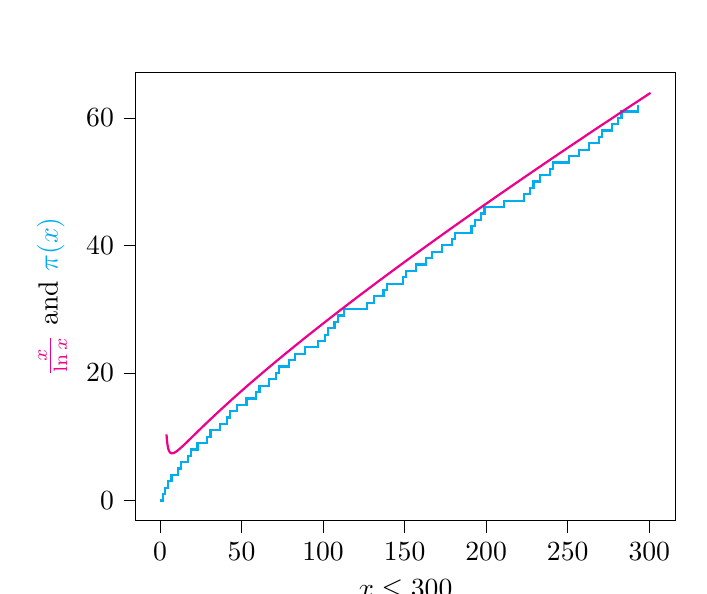
\begin{tikzpicture}

% \definecolor{black}{RGB}{176,176,176}
% \definecolor{magenta}{RGB}{255,127,14}
% \definecolor{cyan}{RGB}{31,119,180}

\begin{axis}[
tick align=outside,
tick pos=left,
x grid style={black},
xlabel={\(\displaystyle x \leq 300\)},
xmin=-15.04, xmax=315.84,
xtick style={color=black},
y grid style={black},
ylabel={$\rt{\frac{x}{\ln x}}$ and $\bt{\pi(x)}$},
ymin=-3.19561752191996, ymax=67.1079679603191,
ytick style={color=black}
]
\addplot [thick, cyan, const plot mark left]
table {%
0 0
2 1
3 2
5 3
7 4
11 5
13 6
17 7
19 8
23 9
29 10
31 11
37 12
41 13
43 14
47 15
53 16
59 17
61 18
67 19
71 20
73 21
79 22
83 23
89 24
97 25
101 26
103 27
107 28
109 29
113 30
127 31
131 32
137 33
139 34
149 35
151 36
157 37
163 38
167 39
173 40
179 41
181 42
191 43
193 44
197 45
199 46
211 47
223 48
227 49
229 50
233 51
239 52
241 53
251 54
257 55
263 56
269 57
271 58
277 59
281 60
283 61
293 62
};
\addplot [thick, magenta]
table {%
4 10.3547977982484
4.2 9.65329667196755
4.4 9.13612648160719
4.6 8.7443111496587
4.8 8.44155052431592
5 8.20428118761098
5.2 8.01654336330027
5.4 7.86714486074388
5.6 7.74800608869024
5.8 7.65314957549306
6 7.57805903584563
6.2 7.5192593817862
6.4 7.47403365651635
6.6 7.44022750321727
6.8 7.41611114139458
7 7.40028004455914
7.2 7.39158222740837
7.4 7.38906418345587
7.6 7.39193012293241
7.8 7.39951084551978
8 7.41123969302713
8.2 7.42663377297653
8.4 7.44527915360876
8.6 7.46681908441012
8.8 7.49094454518631
9 7.51738660429497
9.2 7.54591019490969
9.40000000000001 7.57630901188945
9.6 7.60840130101444
9.8 7.64202636394601
10 7.6770416411066
10.2 7.71332026416685
10.4 7.75074899240532
10.6 7.78922646462551
10.8 7.82866171185321
11 7.86897288663098
11.2 7.91008617307111
11.4 7.95193484844151
11.6 7.99445847233134
11.8 8.03760218366919
12 8.08131608927284
12.2 8.12555473036858
12.4 8.17027661576329
12.6 8.21544381218863
12.8 8.26102158384465
13 8.30697807441319
13.2 8.35328402584184
13.4 8.39991252905441
13.6 8.44683880245882
13.8 8.49403999472043
14 8.54149500877207
14.2 8.58918434445481
14.4 8.63708995754214
14.6 8.6851951332037
14.8 8.73348437222317
15 8.78194328850549
15.2 8.83055851659701
15.4 8.87931762810392
15.6 8.92820905603361
15.8 8.97722202620314
16 9.02634649496301
16.2 9.0755730925738
16.4 9.12489307165138
16.6 9.17429826016389
16.8 9.22378101852308
17 9.27333420036391
17.2 9.32295111665152
17.4 9.37262550279436
17.6 9.42235148847709
17.8 9.47212356995722
18 9.52193658459677
18.2 9.5717856874239
18.4 9.62166632954052
18.6 9.67157423821073
18.8 9.72150539848136
19 9.77145603620079
19.2 9.82142260231508
19.4 9.8714017583326
19.6 9.92139036285822
19.8 9.97138545910797
20 10.0213842633231
20.2 10.0713841540101
20.4 10.1213826619401
20.6 10.1713774608464
20.8 10.221366358766
21 10.2713472899733
21.2 10.3213183074613
21.4 10.3712775759278
21.6 10.4212233652277
21.8 10.4711540442578
22 10.5210680752401
22.2 10.5709640083761
22.4 10.6208404768429
22.6 10.6706961921086
22.8 10.7205299395421
23 10.7703405742978
23.2 10.8201270174553
23.4 10.8698882523958
23.6 10.9196233214005
23.8 10.9693313224532
24 11.019011406236
24.2 11.0686627733029
24.4 11.1182846714206
24.6 11.1678763930656
24.8 11.2174372730655
25 11.2669666863782
25.2 11.3164640459969
25.4 11.365928800975
25.6 11.4153604345624
25.8 11.4647584624463
26 11.5141224310901
26.2 11.5634519161636
26.4 11.6127465210605
26.6 11.6620058754959
26.8 11.7112296341799
27 11.7604174755634
27.2 11.8095691006503
27.4 11.858684231873
27.6 11.9077626120276
27.8 11.9568040032649
28 12.005808186134
28.2 12.0547749586758
28.4 12.1037041355631
28.6 12.1525955472848
28.8 12.2014490393721
29 12.2502644716633
29.2 12.2990417176066
29.4 12.347780663597
29.6 12.3964812083469
29.8 12.445143262288
30 12.4937667470025
30.2 12.542351594682
30.4 12.5908977476139
30.6 12.6394051576919
30.8 12.6878737859501
31 12.7363036021208
31.2 12.7846945842121
31.4 12.8330467181066
31.6 12.8813599971791
31.8 12.9296344219319
32 12.9778699996482
32.2 13.0260667440607
32.4 13.074224675037
32.6 13.1223438182784
32.8 13.1704242050338
33 13.2184658718259
33.2 13.266468860191
33.4 13.3144332164298
33.6 13.3623589913702
33.8 13.4102462401408
34 13.4580950219549
34.2 13.5059053999036
34.4 13.5536774407595
34.6 13.6014112147877
34.8 13.6491067955668
35 13.6967642598167
35.2 13.7443836872349
35.4 13.79196516034
35.6 13.8395087643216
35.8 13.8870145868975
36 13.9344827181771
36.2 13.9819132505305
36.4 14.0293062784635
36.6 14.0766618984986
36.8 14.1239802090606
37 14.1712613103673
37.2 14.2185053043254
37.4 14.2657122944307
37.6 14.3128823856721
37.8 14.3600156844412
38 14.4071122984441
38.2 14.4541723366187
38.4 14.5011959090541
38.6 14.5481831269146
38.8 14.5951341023666
39 14.6420489485084
39.2 14.6889277793038
39.4 14.7357707095175
39.6 14.7825778546544
39.8 14.8293493309007
40 14.8760852550681
40.2 14.9227857445403
40.4 14.9694509172213
40.6 15.0160808914868
40.8 15.0626757861373
41 15.1092357203527
41.2 15.1557608136502
41.4 15.2022511858427
41.6 15.2487069569998
41.8 15.2951282474102
42 15.3415151775457
42.2 15.3878678680273
42.4 15.4341864395921
42.6 15.480471013062
42.8 15.5267217093138
43 15.5729386492508
43.2 15.6191219537749
43.4 15.6652717437612
43.6 15.7113881400326
43.8 15.757471263336
44 15.8035212343197
44.2 15.8495381735118
44.4 15.8955222012993
44.6 15.9414734379083
44.8 15.9873920033855
45 16.0332780175797
45.2 16.0791316001253
45.4 16.1249528704254
45.6 16.1707419476367
45.8 16.2164989506545
46 16.2622239980986
46.2 16.3079172082998
46.4 16.3535786992876
46.6 16.3992085887775
46.8 16.4448069941598
47 16.4903740324889
47.2 16.5359098204723
47.4 16.5814144744613
47.6 16.6268881104415
47.8 16.6723308440239
48 16.7177427904367
48.2 16.7631240645173
48.4 16.8084747807047
48.6 16.8537950530328
48.8 16.8990849951233
49 16.94434472018
49.2 16.9895743409822
49.4 17.0347739698799
49.6 17.0799437187881
49.8 17.1250836991822
50 17.1701940220931
50.2 17.2152747981036
50.4 17.2603261373437
50.6 17.3053481494874
50.8 17.3503409437491
51 17.3953046288805
51.2 17.4402393131678
51.4 17.4851451044286
51.6 17.5300221100101
51.8 17.5748704367862
52 17.619690191156
52.2 17.6644814790417
52.4 17.7092444058871
52.6 17.7539790766559
52.8 17.7986855958307
53 17.8433640674119
53.2 17.8880145949166
53.4 17.9326372813778
53.6 17.977232229344
53.8 18.0217995408784
54 18.0663393175588
54.2 18.1108516604771
54.4 18.1553366702395
54.6 18.1997944469664
54.8 18.2442250902923
55 18.2886286993666
55.2 18.3330053728532
55.4 18.3773552089316
55.6 18.4216783052972
55.8 18.4659747591618
56 18.5102446672546
56.2 18.5544881258228
56.4 18.5987052306324
56.6 18.6428960769696
56.8 18.6870607596415
57 18.7311993729772
57.2 18.775312010829
57.4 18.8193987665739
57.6000000000001 18.8634597331145
57.8 18.9074950028806
58 18.9515046678306
58.2 18.995488819453
58.4 19.0394475487678
58.6000000000001 19.0833809463281
58.8 19.1272891022217
59 19.1711721060728
59.2 19.2150300470438
59.4 19.2588630138366
59.6000000000001 19.302671094695
59.8 19.3464543774059
60 19.3902129493016
60.2000000000001 19.4339468972614
60.4 19.4776563077134
60.6000000000001 19.5213412666368
60.8000000000001 19.5650018595635
61 19.6086381715802
61.2000000000001 19.6522502873305
61.4 19.6958382910166
61.6000000000001 19.7394022664016
61.8000000000001 19.7829422968116
62 19.8264584651376
62.2000000000001 19.8699508538374
62.4 19.9134195449383
62.6000000000001 19.9568646200385
62.8000000000001 20.0002861603099
63 20.0436842464997
63.2000000000001 20.0870589589327
63.4000000000001 20.1304103775137
63.6000000000001 20.1737385817293
63.8000000000001 20.2170436506503
64.0000000000001 20.260325662934
64.2 20.3035846968259
64.4000000000001 20.3468208301625
64.6000000000001 20.3900341403729
64.8000000000001 20.4332247044815
65.0000000000001 20.47639259911
65.2 20.5195379004795
65.4000000000001 20.5626606844128
65.6000000000001 20.6057610263367
65.8000000000001 20.648839001284
66.0000000000001 20.6918946838959
66.2 20.7349281484242
66.4000000000001 20.7779394687332
66.6000000000001 20.8209287183024
66.8000000000001 20.8638959702282
67.0000000000001 20.9068412972265
67.2000000000001 20.9497647716346
67.4000000000001 20.9926664654136
67.6000000000001 21.0355464501505
67.8000000000001 21.0784047970603
68.0000000000001 21.1212415769884
68.2000000000001 21.1640568604124
68.4000000000001 21.2068507174448
68.6000000000001 21.2496232178347
68.8000000000001 21.29237443097
69.0000000000001 21.3351044258799
69.2000000000001 21.3778132712367
69.4000000000001 21.4205010353581
69.6000000000001 21.463167786209
69.8000000000001 21.5058135914044
70.0000000000001 21.5484385182105
70.2000000000001 21.5910426335477
70.4000000000001 21.6336260039919
70.6000000000001 21.6761886957775
70.8000000000001 21.7187307747985
71.0000000000001 21.7612523066114
71.2000000000001 21.8037533564368
71.4000000000001 21.8462339891613
71.6000000000001 21.8886942693403
71.8000000000001 21.9311342611992
72.0000000000001 21.9735540286359
72.2000000000001 22.0159536352227
72.4000000000001 22.0583331442081
72.6000000000001 22.1006926185194
72.8000000000001 22.1430321207639
73.0000000000001 22.1853517132314
73.2000000000001 22.2276514578962
73.4000000000001 22.2699314164185
73.6000000000001 22.3121916501471
73.8000000000001 22.3544322201209
74.0000000000001 22.3966531870706
74.2000000000001 22.4388546114214
74.4000000000001 22.4810365532941
74.6000000000001 22.5231990725074
74.8000000000001 22.5653422285797
75.0000000000001 22.6074660807309
75.2000000000001 22.6495706878845
75.4000000000001 22.6916561086693
75.6000000000001 22.733722401421
75.8000000000001 22.7757696241845
76.0000000000001 22.8177978347155
76.2000000000001 22.8598070904821
76.4000000000001 22.901797448667
76.6000000000001 22.943768966169
76.8000000000001 22.985721699605
77.0000000000001 23.0276557053114
77.2000000000001 23.0695710393462
77.4000000000001 23.1114677574908
77.6000000000001 23.1533459152514
77.8000000000001 23.1952055678609
78.0000000000001 23.2370467702807
78.2000000000001 23.2788695772022
78.4000000000001 23.3206740430489
78.6000000000001 23.3624602219773
78.8000000000001 23.4042281678795
79.0000000000001 23.4459779343842
79.2000000000001 23.4877095748587
79.4000000000001 23.5294231424103
79.6000000000001 23.5711186898881
79.8000000000001 23.6127962698845
80.0000000000001 23.654455934737
80.2000000000001 23.6960977365294
80.4000000000001 23.737721727094
80.6000000000001 23.7793279580125
80.8000000000001 23.820916480618
81.0000000000001 23.8624873459966
81.2000000000001 23.9040406049886
81.4000000000001 23.9455763081903
81.6000000000001 23.9870945059553
81.8000000000001 24.0285952483964
82.0000000000001 24.0700785853867
82.2000000000001 24.1115445665613
82.4000000000001 24.1529932413188
82.6000000000001 24.1944246588226
82.8000000000001 24.2358388680026
83.0000000000001 24.2772359175564
83.2000000000001 24.318615855951
83.4000000000001 24.3599787314241
83.6000000000001 24.4013245919853
83.8000000000001 24.4426534854181
84.0000000000001 24.4839654592808
84.2000000000001 24.525260560908
84.4000000000001 24.566538837412
84.6000000000001 24.6078003356844
84.8000000000001 24.6490451023971
85.0000000000001 24.6902731840039
85.2000000000001 24.7314846267417
85.4000000000001 24.7726794766321
85.6000000000001 24.8138577794823
85.8000000000001 24.8550195808869
86.0000000000001 24.8961649262289
86.2000000000001 24.9372938606809
86.4000000000001 24.9784064292069
86.6000000000001 25.0195026765629
86.8000000000001 25.0605826472989
87.0000000000001 25.1016463857594
87.2000000000001 25.1426939360854
87.4000000000001 25.1837253422151
87.6000000000001 25.2247406478853
87.8000000000001 25.2657398966329
88.0000000000001 25.3067231317956
88.2000000000001 25.3476903965136
88.4000000000001 25.3886417337306
88.6000000000001 25.4295771861948
88.8000000000001 25.4704967964605
89.0000000000001 25.5114006068891
89.2000000000001 25.5522886596501
89.4000000000001 25.5931609967224
89.6000000000001 25.6340176598956
89.8000000000001 25.6748586907708
90.0000000000001 25.7156841307622
90.2000000000001 25.7564940210977
90.4000000000001 25.7972884028205
90.6000000000001 25.8380673167899
90.8000000000001 25.8788308036827
91.0000000000001 25.9195789039937
91.2000000000001 25.9603116580378
91.4000000000001 26.0010291059499
91.6000000000001 26.041731287687
91.8000000000001 26.0824182430287
92.0000000000001 26.1230900115782
92.2000000000001 26.1637466327639
92.4000000000001 26.2043881458398
92.6000000000001 26.245014589887
92.8000000000001 26.2856260038145
93.0000000000001 26.3262224263602
93.2000000000001 26.3668038960923
93.4000000000001 26.4073704514097
93.6000000000001 26.4479221305434
93.8000000000001 26.4884589715575
94.0000000000001 26.5289810123501
94.2000000000001 26.5694882906541
94.4000000000001 26.6099808440385
94.6000000000001 26.6504587099093
94.8000000000001 26.6909219255102
95.0000000000001 26.7313705279238
95.2000000000001 26.7718045540725
95.4000000000001 26.8122240407196
95.6000000000001 26.8526290244696
95.8000000000001 26.8930195417701
96.0000000000001 26.933395628912
96.2000000000001 26.9737573220304
96.4000000000001 27.014104657106
96.6000000000001 27.0544376699658
96.8000000000001 27.0947563962836
97.0000000000001 27.1350608715815
97.2000000000001 27.1753511312304
97.4000000000001 27.2156272104509
97.6000000000001 27.2558891443144
97.8000000000001 27.2961369677437
98.0000000000001 27.3363707155139
98.2000000000001 27.3765904222536
98.4000000000001 27.416796122445
98.6000000000001 27.4569878504257
98.8000000000001 27.4971656403888
99.0000000000001 27.5373295263839
99.2000000000001 27.5774795423181
99.4000000000001 27.6176157219567
99.6000000000001 27.6577380989241
99.8000000000001 27.6978467067043
100 27.7379415786421
100.2 27.7780227479438
100.4 27.8180902476776
100.6 27.8581441107751
100.8 27.8981843700313
101 27.9382110581059
101.2 27.9782242075241
101.4 28.0182238506768
101.6 28.0582100198221
101.8 28.0981827470854
102 28.1381420644606
102.2 28.1780880038105
102.4 28.218020596868
102.6 28.2579398752363
102.8 28.2978458703899
103 28.3377386136753
103.2 28.3776181363118
103.4 28.417484469392
103.6 28.4573376438827
103.8 28.4971776906254
104 28.5370046403372
104.2 28.5768185236115
104.4 28.6166193709184
104.6 28.6564072126058
104.8 28.6961820788997
105 28.7359439999051
105.2 28.7756930056065
105.4 28.8154291258689
105.6 28.8551523904379
105.8 28.894862828941
106 28.9345604708878
106.2 28.9742453456707
106.4 29.0139174825657
106.6 29.0535769107329
106.8 29.0932236592172
107 29.1328577569492
107.2 29.172479232745
107.4 29.2120881153078
107.6 29.2516844332279
107.8 29.2912682149836
108 29.3308394889416
108.2 29.3703982833577
108.4 29.4099446263775
108.6 29.4494785460369
108.8 29.4890000702625
109 29.5285092268727
109.2 29.5680060435776
109.4 29.6074905479802
109.6 29.6469627675767
109.8 29.686422729757
110 29.7258704618055
110.2 29.7653059909014
110.4 29.8047293441193
110.6 29.8441405484302
110.8 29.8835396307012
111 29.9229266176971
111.2 29.9623015360799
111.4 30.0016644124102
111.6 30.0410152731472
111.8 30.0803541446494
112 30.1196810531752
112.2 30.1589960248833
112.4 30.1982990858336
112.6 30.2375902619869
112.8 30.2768695792064
113 30.3161370632576
113.2 30.3553927398088
113.4 30.394636634432
113.6 30.4338687726031
113.8 30.4730891797024
114 30.5122978810153
114.2 30.5514949017326
114.4 30.5906802669511
114.6 30.6298540016741
114.8 30.6690161308116
115 30.7081666791814
115.2 30.7473056715088
115.4 30.7864331324277
115.6 30.8255490864809
115.8 30.8646535581204
116 30.903746571708
116.2 30.9428281515157
116.4 30.9818983217264
116.6 31.0209571064339
116.8 31.0600045296439
117 31.0990406152739
117.2 31.138065387154
117.4 31.1770788690275
117.6 31.2160810845509
117.8 31.2550720572944
118 31.2940518107429
118.2 31.3330203682956
118.4 31.3719777532672
118.6 31.4109239888878
118.8 31.4498590983035
119 31.4887831045769
119.2 31.5276960306875
119.4 31.566597899532
119.6 31.6054887339248
119.8 31.6443685565983
120 31.6832373902037
120.2 31.722095257311
120.4 31.7609421804093
120.6 31.7997781819077
120.8 31.8386032841353
121 31.8774175093419
121.2 31.9162208796981
121.4 31.9550134172956
121.6 31.9937951441483
121.8 32.0325660821918
122 32.0713262532844
122.2 32.1100756792071
122.4 32.1488143816642
122.6 32.1875423822837
122.8 32.2262597026176
123 32.2649663641422
123.2 32.3036623882585
123.4 32.3423477962927
123.6 32.3810226094966
123.8 32.4196868490475
124 32.4583405360494
124.2 32.4969836915323
124.4 32.5356163364536
124.6 32.5742384916978
124.8 32.612850178077
125 32.6514514163314
125.2 32.6900422271293
125.4 32.728622631068
125.6 32.7671926486735
125.8 32.8057523004016
126 32.8443016066373
126.2 32.8828405876961
126.4 32.9213692638235
126.6 32.9598876551961
126.8 32.9983957819213
127 33.0368936640379
127.2 33.0753813215165
127.4 33.1138587742597
127.6 33.1523260421024
127.8 33.1907831448124
128 33.2292301020902
128.2 33.2676669335698
128.4 33.3060936588189
128.6 33.344510297339
128.8 33.3829168685661
129 33.4213133918704
129.2 33.4596998865573
129.4 33.4980763718673
129.6 33.5364428669765
129.8 33.5747993909966
130 33.6131459629756
130.2 33.6514826018978
130.4 33.6898093266842
130.6 33.7281261561929
130.8 33.7664331092192
131 33.804730204496
131.2 33.8430174606942
131.4 33.8812948964226
131.6 33.9195625302288
131.8 33.9578203805989
132 33.9960684659581
132.2 34.0343068046709
132.4 34.0725354150415
132.6 34.1107543153138
132.8 34.1489635236718
133 34.1871630582403
133.2 34.2253529370844
133.4 34.2635331782103
133.6 34.3017037995656
133.8 34.3398648190391
134 34.3780162544617
134.2 34.4161581236061
134.4 34.4542904441875
134.6 34.4924132338636
134.8 34.5305265102349
135 34.5686302908451
135.2 34.6067245931811
135.4 34.6448094346735
135.6 34.6828848326969
135.8 34.7209508045698
136 34.7590073675551
136.2 34.7970545388607
136.4 34.8350923356388
136.6 34.8731207749871
136.8 34.9111398739487
137 34.9491496495121
137.2 34.9871501186118
137.4 35.0251412981285
137.6 35.063123204889
137.8 35.1010958556669
138 35.1390592671826
138.2 35.1770134561034
138.4 35.2149584390441
138.6 35.2528942325671
138.8 35.2908208531823
139 35.3287383173477
139.2 35.3666466414697
139.4 35.404545841903
139.6 35.4424359349511
139.8 35.4803169368662
140 35.5181888638499
140.2 35.556051732053
140.4 35.5939055575761
140.6 35.6317503564693
140.8 35.6695861447331
141 35.7074129383179
141.2 35.7452307531248
141.4 35.7830396050054
141.6 35.8208395097625
141.8 35.8586304831498
142 35.8964125408724
142.2 35.9341856985868
142.4 35.9719499719014
142.6 36.0097053763767
142.8 36.0474519275251
143 36.0851896408114
143.2 36.1229185316533
143.4 36.160638615421
143.6 36.1983499074377
143.8 36.2360524229798
144 36.2737461772774
144.2 36.3114311855139
144.4 36.3491074628265
144.6 36.3867750243065
144.8 36.4244338849994
145 36.4620840599051
145.2 36.499725563978
145.4 36.5373584121274
145.6 36.5749826192175
145.8 36.6125982000676
146 36.6502051694525
146.2 36.6878035421025
146.4 36.7253933327037
146.6 36.7629745558979
146.8 36.8005472262833
147 36.8381113584142
147.2 36.8756669668015
147.4 36.9132140659127
147.6 36.9507526701722
147.8 36.9882827939613
148 37.0258044516187
148.2 37.0633176574403
148.4 37.1008224256798
148.6 37.1383187705485
148.8 37.1758067062156
149 37.2132862468086
149.2 37.2507574064129
149.4 37.2882201990728
149.6 37.3256746387908
149.8 37.3631207395286
150 37.4005585152067
150.2 37.4379879797045
150.4 37.4754091468611
150.6 37.5128220304749
150.8 37.5502266443038
151 37.5876230020659
151.2 37.6250111174388
151.4 37.6623910040607
151.6 37.6997626755297
151.8 37.7371261454047
152 37.7744814272051
152.2 37.811828534411
152.4 37.8491674804636
152.6 37.8864982787653
152.8 37.9238209426794
153 37.961135485531
153.2 37.9984419206067
153.4 38.0357402611547
153.6 38.0730305203854
153.8 38.1103127114709
154 38.1475868475458
154.2 38.184852941707
154.4 38.2221110070138
154.6 38.2593610564882
154.8 38.2966031031152
155 38.3338371598426
155.2 38.3710632395814
155.4 38.4082813552058
155.6 38.4454915195534
155.8 38.4826937454255
156 38.519888045587
156.2 38.5570744327667
156.4 38.5942529196575
156.6 38.6314235189162
156.8 38.668586243164
157 38.7057411049868
157.2 38.7428881169346
157.4 38.7800272915225
157.6 38.8171586412302
157.8 38.8542821785027
158 38.8913979157497
158.2 38.9285058653466
158.4 38.965606039634
158.6 39.0026984509181
158.8 39.0397831114707
159 39.0768600335295
159.2 39.1139292292982
159.4 39.1509907109465
159.6 39.1880444906103
159.8 39.2250905803921
160 39.2621289923604
160.2 39.2991597385509
160.4 39.3361828309656
160.6 39.3731982815736
160.8 39.410206102311
161 39.447206305081
161.2 39.484198901754
161.4 39.5211839041679
161.6 39.558161324128
161.8 39.5951311734075
162 39.6320934637471
162.2 39.6690482068556
162.4 39.7059954144096
162.6 39.742935098054
162.8 39.779867269402
163 39.8167919400352
163.2 39.8537091215035
163.4 39.8906188253257
163.6 39.9275210629892
163.8 39.9644158459504
164 40.0013031856345
164.2 40.0381830934361
164.4 40.0750555807187
164.6 40.1119206588154
164.8 40.1487783390288
165 40.1856286326308
165.2 40.2224715508633
165.4 40.2593071049379
165.6 40.2961353060361
165.8 40.3329561653095
166 40.3697696938799
166.2 40.4065759028392
166.4 40.4433748032498
166.6 40.4801664061447
166.8 40.5169507225274
167 40.5537277633722
167.2 40.590497539624
167.4 40.6272600621989
167.6 40.6640153419839
167.8 40.7007633898374
168 40.7375042165887
168.2 40.7742378330388
168.4 40.81096424996
168.6 40.8476834780962
168.8 40.8843955281631
169 40.9211004108482
169.2 40.9577981368108
169.4 40.9944887166823
169.6 41.0311721610661
169.8 41.0678484805381
170 41.1045176856461
170.2 41.1411797869108
170.4 41.177834794825
170.6 41.2144827198544
170.8 41.2511235724374
171 41.2877573629852
171.2 41.3243841018819
171.4 41.3610037994846
171.6 41.3976164661237
171.8 41.4342221121027
172 41.4708207476985
172.2 41.5074123831613
172.4 41.543997028715
172.6 41.580574694557
172.8 41.6171453908586
173 41.6537091277646
173.2 41.690265915394
173.4 41.7268157638397
173.6 41.7633586831687
173.8 41.7998946834222
174 41.8364237746157
174.2 41.8729459667391
174.4 41.9094612697567
174.6 41.9459696936076
174.8 41.9824712482052
175 42.0189659434379
175.2 42.055453789169
175.4 42.0919347952365
175.6 42.1284089714537
175.8 42.1648763276088
176 42.2013368734652
176.2 42.2377906187618
176.4 42.2742375732128
176.6 42.3106777465078
176.8 42.3471111483119
177 42.3835377882661
177.2 42.4199576759869
177.4 42.4563708210667
177.6 42.4927772330739
177.8 42.5291769215528
178 42.5655698960238
178.2 42.6019561659834
178.4 42.6383357409044
178.6 42.6747086302361
178.8 42.711074843404
179 42.7474343898102
179.2 42.7837872788333
179.4 42.8201335198286
179.6 42.8564731221283
179.8 42.8928060950413
180 42.9291324478534
180.2 42.9654521898274
180.4 43.0017653302033
180.6 43.0380718781981
180.8 43.0743718430061
181 43.110665233799
181.2 43.1469520597258
181.4 43.183232329913
181.6 43.2195060534647
181.8 43.2557732394625
182 43.2920338969659
182.2 43.3282880350121
182.4 43.3645356626162
182.6 43.4007767887711
182.8 43.437011422448
183 43.4732395725959
183.2 43.5094612481422
183.4 43.5456764579924
183.6 43.5818852110305
183.8 43.6180875161188
184 43.6542833820979
184.2 43.6904728177873
184.4 43.7266558319848
184.6 43.7628324334672
184.8 43.7990026309898
185 43.8351664332869
185.2 43.8713238490717
185.4 43.9074748870363
185.6 43.943619555852
185.8 43.9797578641691
186 44.0158898206173
186.2 44.0520154338052
186.4 44.0881347123213
186.6 44.124247664733
186.8 44.1603542995874
187 44.1964546254112
187.2 44.2325486507107
187.4 44.2686363839719
187.6 44.3047178336605
187.8 44.340793008222
188 44.376861916082
188.2 44.4129245656459
188.4 44.4489809652993
188.6 44.4850311234076
188.8 44.5210750483167
189 44.5571127483525
189.2 44.5931442318214
189.4 44.6291695070101
189.6 44.6651885821857
189.8 44.7012014655958
190 44.7372081654687
190.2 44.7732086900131
190.4 44.8092030474186
190.6 44.8451912458555
190.8 44.8811732934749
191 44.9171491984089
191.2 44.9531189687704
191.4 44.9890826126534
191.6 45.0250401381331
191.8 45.0609915532656
192 45.0969368660883
192.2 45.1328760846201
192.4 45.1688092168609
192.6 45.2047362707921
192.8 45.2406572543768
193 45.2765721755592
193.2 45.3124810422654
193.4 45.348383862403
193.6 45.3842806438614
193.8 45.4201713945116
194 45.4560561222066
194.2 45.4919348347812
194.4 45.5278075400521
194.6 45.5636742458181
194.8 45.5995349598599
195 45.6353896899405
195.2 45.6712384438049
195.4 45.7070812291806
195.6 45.7429180537771
195.8 45.7787489252864
196 45.8145738513829
196.2 45.8503928397234
196.4 45.8862058979473
196.6 45.9220130336765
196.8 45.9578142545157
197 45.9936095680521
197.2 46.0293989818558
197.4 46.0651825034795
197.6 46.100960140459
197.8 46.1367319003128
198 46.1724977905426
198.2 46.2082578186329
198.4 46.2440119920515
198.6 46.2797603182491
198.8 46.3155028046598
199 46.3512394587007
199.2 46.3869702877725
199.4 46.4226952992591
199.6 46.4584145005277
199.8 46.4941278989291
200 46.5298355017976
200.2 46.565537316451
200.4 46.6012333501908
200.6 46.636923610302
200.8 46.6726081040535
201 46.708286838698
201.2 46.7439598214718
201.4 46.7796270595952
201.6 46.8152885602724
201.8 46.8509443306918
202 46.8865943780255
202.2 46.9222387094298
202.4 46.9578773320451
202.6 46.9935102529962
202.8 47.0291374793917
203 47.064759018325
203.2 47.1003748768733
203.4 47.1359850620986
203.6 47.1715895810471
203.8 47.2071884407495
204 47.2427816482211
204.2 47.2783692104617
204.4 47.3139511344559
204.6 47.3495274271726
204.8 47.3850980955657
205 47.4206631465739
205.2 47.4562225871206
205.4 47.491776424114
205.6 47.5273246644474
205.8 47.5628673149988
206 47.5984043826314
206.2 47.6339358741935
206.4 47.6694617965182
206.6 47.704982156424
206.8 47.7404969607145
207 47.7760062161786
207.2 47.8115099295904
207.4 47.8470081077093
207.6 47.8825007572801
207.8 47.9179878850332
208 47.953469497684
208.2 47.988945601934
208.4 48.0244162044697
208.6 48.0598813119636
208.8 48.0953409310735
209 48.1307950684432
209.2 48.1662437307021
209.4 48.2016869244652
209.6 48.2371246563336
209.8 48.2725569328941
210 48.3079837607193
210.2 48.343405146368
210.4 48.3788210963847
210.6 48.4142316173003
210.8 48.4496367156313
211 48.4850363978807
211.2 48.5204306705374
211.4 48.5558195400768
211.6 48.5912030129601
211.8 48.6265810956353
212 48.6619537945362
212.2 48.6973211160834
212.4 48.7326830666836
212.6 48.7680396527302
212.8 48.8033908806028
213 48.8387367566678
213.2 48.874077287278
213.4 48.9094124787728
213.6 48.9447423374785
213.8 48.9800668697077
214 49.01538608176
214.2 49.0506999799218
214.4 49.086008570466
214.6 49.1213118596527
214.8 49.1566098537287
215 49.1919025589278
215.2 49.2271899814706
215.4 49.2624721275651
215.6 49.2977490034058
215.8 49.3330206151748
216 49.3682869690409
216.2 49.4035480711603
216.4 49.4388039276764
216.6 49.4740545447198
216.8 49.5092999284082
217 49.5445400848469
217.2 49.5797750201283
217.4 49.6150047403324
217.6 49.6502292515264
217.8 49.6854485597652
218 49.720662671091
218.2 49.7558715915336
218.4 49.7910753271103
218.6 49.8262738838263
218.8 49.8614672676741
219 49.8966554846339
219.2 49.9318385406739
219.4 49.9670164417498
219.6 50.0021891938052
219.8 50.0373568027714
220 50.0725192745677
220.2 50.1076766151012
220.4 50.1428288302671
220.6 50.1779759259483
220.8 50.2131179080159
221 50.2482547823289
221.2 50.2833865547346
221.4 50.318513231068
221.6 50.3536348171527
221.8 50.3887513188002
222 50.4238627418102
222.2 50.4589690919708
222.4 50.4940703750582
222.6 50.5291665968371
222.8 50.5642577630603
223 50.5993438794692
223.2 50.6344249517936
223.4 50.6695009857515
223.6 50.7045719870497
223.8 50.7396379613833
224 50.7746989144361
224.2 50.8097548518802
224.4 50.8448057793765
224.6 50.8798517025748
224.8 50.914892627113
225 50.9499285586182
225.2 50.9849595027059
225.4 51.0199854649808
225.6 51.0550064510358
225.8 51.0900224664532
226 51.1250335168039
226.2 51.1600396076476
226.4 51.1950407445332
226.6 51.2300369329984
226.8 51.2650281785699
227 51.3000144867635
227.2 51.3349958630839
227.4 51.369972313025
227.6 51.4049438420699
227.8 51.4399104556907
228 51.4748721593488
228.2 51.5098289584946
228.4 51.544780858568
228.6 51.5797278649981
228.8 51.6146699832031
229 51.6496072185909
229.2 51.6845395765583
229.4 51.7194670624919
229.6 51.7543896817676
229.8 51.7893074397506
230 51.8242203417957
230.2 51.8591283932473
230.4 51.8940315994392
230.6 51.9289299656947
230.8 51.963823497327
231 51.9987121996386
231.2 52.0335960779218
231.4 52.0684751374586
231.6 52.1033493835207
231.8 52.1382188213696
232 52.1730834562563
232.2 52.2079432934219
232.4 52.2427983380973
232.6 52.2776485955031
232.8 52.3124940708498
233 52.347334769338
233.2 52.382170696158
233.4 52.4170018564903
233.6 52.4518282555051
233.8 52.486649898363
234 52.5214667902143
234.2 52.5562789361996
234.4 52.5910863414495
234.6 52.6258890110847
234.8 52.6606869502162
235 52.695480163945
235.2 52.7302686573626
235.4 52.7650524355504
235.6 52.7998315035802
235.8 52.8346058665142
236 52.8693755294049
236.2 52.9041404972949
236.4 52.9389007752175
236.6 52.9736563681961
236.8 53.0084072812449
237 53.0431535193681
237.2 53.0778950875607
237.4 53.1126319908081
237.6 53.1473642340863
237.8 53.1820918223617
238 53.2168147605914
238.2 53.2515330537231
238.4 53.286246706695
238.6 53.3209557244362
238.8 53.3556601118663
239 53.3903598738956
239.2 53.4250550154252
239.4 53.459745541347
239.6 53.4944314565435
239.8 53.5291127658882
240 53.5637894742454
240.2 53.5984615864702
240.4 53.6331291074085
240.6 53.6677920418973
240.8 53.7024503947645
241 53.7371041708286
241.2 53.7717533748997
241.4 53.8063980117783
241.6 53.8410380862563
241.8 53.8756736031165
242 53.9103045671329
242.2 53.9449309830705
242.4 53.9795528556853
242.6 54.0141701897247
242.8 54.0487829899272
243 54.0833912610222
243.2 54.1179950077308
243.4 54.152594234765
243.6 54.1871889468282
243.8 54.2217791486149
244 54.2563648448112
244.2 54.2909460400944
244.4 54.325522739133
244.6 54.3600949465871
244.8 54.3946626671081
245 54.4292259053388
245.2 54.4637846659136
245.4 54.4983389534581
245.6 54.5328887725897
245.8 54.567434127917
246 54.6019750240403
246.2 54.6365114655516
246.4 54.6710434570342
246.6 54.7055710030631
246.8 54.7400941082051
247 54.7746127770183
247.2 54.8091270140528
247.4 54.8436368238502
247.6 54.8781422109439
247.8 54.912643179859
248 54.9471397351123
248.2 54.9816318812125
248.4 55.0161196226599
248.6 55.0506029639469
248.8 55.0850819095575
249 55.1195564639675
249.2 55.154026631645
249.4 55.1884924170495
249.6 55.2229538246328
249.8 55.2574108588385
250 55.291863524102
250.2 55.3263118248509
250.4 55.3607557655049
250.6 55.3951953504754
250.8 55.4296305841662
251 55.4640614709729
251.2 55.4984880152833
251.4 55.5329102214772
251.6 55.5673280939269
251.8 55.6017416369963
252 55.6361508550419
252.2 55.6705557524121
252.4 55.7049563334479
252.6 55.7393526024821
252.8 55.7737445638399
253 55.8081322218389
253.2 55.8425155807889
253.4 55.8768946449919
253.6 55.9112694187424
253.8 55.9456399063272
254 55.9800061120254
254.2 56.0143680401086
254.4 56.0487256948407
254.6 56.083079080478
254.8 56.1174282012694
255 56.1517730614562
255.2 56.1861136652722
255.4 56.2204500169435
255.6 56.254782120689
255.8 56.28910998072
256 56.3234336012404
256.2 56.3577529864467
256.4 56.3920681405279
256.6 56.4263790676658
256.8 56.4606857720346
257 56.4949882578013
257.2 56.5292865291256
257.4 56.5635805901597
257.6 56.5978704450488
257.8 56.6321560979306
258 56.6664375529355
258.2 56.700714814187
258.4 56.734987885801
258.6 56.7692567718864
258.8 56.8035214765449
259 56.837782003871
259.2 56.872038357952
259.4 56.9062905428682
259.6 56.9405385626927
259.8 56.9747824214915
260 57.0090221233237
260.2 57.043257672241
260.4 57.0774890722884
260.6 57.1117163275037
260.8 57.1459394419177
261 57.1801584195543
261.2 57.2143732644303
261.4 57.2485839805557
261.6 57.2827905719334
261.8 57.3169930425595
262 57.3511913964231
262.2 57.3853856375066
262.4 57.4195757697853
262.6 57.4537617972278
262.8 57.4879437237959
263 57.5221215534444
263.2 57.5562952901214
263.4 57.5904649377683
263.6 57.6246305003196
263.8 57.6587919817031
264 57.69294938584
264.2 57.7271027166444
264.4 57.7612519780242
264.6 57.7953971738803
264.8 57.829538308107
265 57.8636753845919
265.2 57.897808407216
265.4 57.9319373798538
265.6 57.966062306373
265.8 58.0001831906349
266 58.0343000364941
266.2 58.0684128477986
266.4 58.10252162839
266.6 58.1366263821034
266.8 58.1707271127672
267 58.2048238242035
267.2 58.2389165202277
267.4 58.2730052046491
267.6 58.3070898812702
267.8 58.3411705538873
268 58.3752472262901
268.2 58.409319902262
268.4 58.4433885855802
268.6 58.4774532800151
268.8 58.5115139893312
269 58.5455707172864
269.2 58.5796234676324
269.4 58.6136722441144
269.6 58.6477170504716
269.8 58.6817578904367
270 58.7157947677362
270.2 58.7498276860905
270.4 58.7838566492135
270.6 58.817881660813
270.8 58.8519027245908
271 58.8859198442421
271.2 58.9199330234564
271.4 58.9539422659167
271.6 58.9879475753
271.8 59.0219489552772
272 59.0559464095129
272.2 59.0899399416658
272.4 59.1239295553885
272.6 59.1579152543275
272.8 59.1918970421231
273 59.2258749224098
273.2 59.2598488988159
273.4 59.2938189749639
273.6 59.32778515447
273.8 59.3617474409447
274 59.3957058379923
274.2 59.4296603492113
274.4 59.4636109781942
274.6 59.4975577285277
274.8 59.5315006037923
275 59.5654396075629
275.2 59.5993747434084
275.4 59.6333060148918
275.6 59.6672334255702
275.8 59.7011569789951
276 59.7350766787118
276.2 59.76899252826
276.4 59.8029045311738
276.6 59.8368126909811
276.8 59.8707170112043
277 59.9046174953598
277.2 59.9385141469587
277.4 59.9724069695058
277.6 60.0062959665006
277.8 60.0401811414367
278 60.0740624978022
278.2 60.1079400390791
278.4 60.1418137687443
278.6 60.1756836902685
278.8 60.2095498071172
279 60.2434121227501
279.2 60.2772706406211
279.4 60.3111253641788
279.6 60.344976296866
279.8 60.3788234421201
280 60.4126668033728
280.2 60.4465063840503
280.4 60.4803421875732
280.6 60.5141742173567
280.8 60.5480024768104
281 60.5818269693385
281.2 60.6156476983395
281.4 60.6494646672067
281.6 60.6832778793277
281.8 60.7170873380847
282 60.7508930468548
282.2 60.7846950090091
282.4 60.8184932279137
282.6 60.8522877069292
282.8 60.8860784494108
283 60.9198654587084
283.2 60.9536487381663
283.4 60.9874282911237
283.6 61.0212041209145
283.8 61.054976230867
284 61.0887446243044
284.2 61.1225093045446
284.4 61.1562702749001
284.6 61.1900275386783
284.8 61.223781099181
285 61.2575309597052
285.2 61.2912771235423
285.4 61.3250195939786
285.6 61.3587583742952
285.8 61.3924934677681
286 61.4262248776678
286.2 61.45995260726
286.4 61.4936766598049
286.6 61.5273970385578
286.8 61.5611137467686
287 61.5948267876823
287.2 61.6285361645387
287.4 61.6622418805725
287.6 61.6959439390131
287.8 61.7296423430852
288 61.7633370960081
288.2 61.7970282009962
288.4 61.8307156612587
288.6 61.8643994799999
288.8 61.8980796604191
289 61.9317562057105
289.2 61.9654291190632
289.4 61.9990984036614
289.6 62.0327640626845
289.8 62.0664260993065
290 62.1000845166968
290.2 62.1337393180197
290.4 62.1673905064346
290.6 62.201038085096
290.8 62.2346820571533
291 62.2683224257513
291.2 62.3019591940297
291.4 62.3355923651233
291.6 62.369221942162
291.8 62.4028479282711
292 62.4364703265707
292.2 62.4700891401763
292.4 62.5037043721984
292.6 62.5373160257428
292.8 62.5709241039105
293 62.6045286097976
293.2 62.6381295464955
293.4 62.6717269170908
293.6 62.7053207246653
293.8 62.738910972296
294 62.7724976630552
294.2 62.8060808000107
294.4 62.8396603862251
294.6 62.8732364247566
294.8 62.9068089186587
295 62.9403778709802
295.2 62.973943284765
295.4 63.0075051630525
295.6 63.0410635088775
295.8 63.07461832527
296 63.1081696152555
296.2 63.1417173818548
296.4 63.1752616280839
296.6 63.2088023569545
296.8 63.2423395714735
297 63.2758732746433
297.2 63.3094034694617
297.4 63.3429301589218
297.6 63.3764533460123
297.8 63.4099730337173
298 63.4434892250164
298.2 63.4770019228845
298.4 63.5105111302922
298.6 63.5440168502054
298.8 63.5775190855856
299 63.6110178393898
299.2 63.6445131145706
299.4 63.6780049140758
299.6 63.7114932408492
299.8 63.7449780978298
300 63.7784594879522
300.2 63.8119374141468
300.4 63.8454118793393
300.6 63.8788828864511
300.8 63.9123504383992
};
\end{axis}

\end{tikzpicture}

    % This file was created with tikzplotlib v0.10.1.
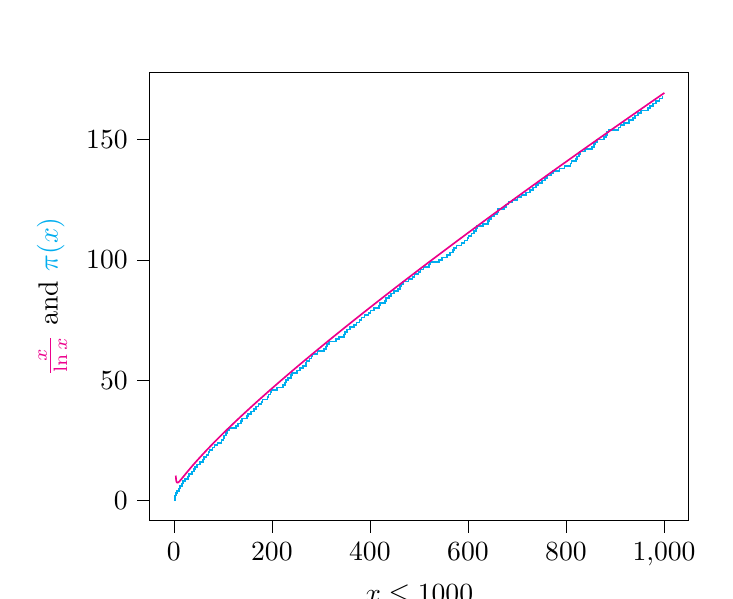
\begin{tikzpicture}%[x=0.75pt,y=0.75pt,yscale=1.1,xscale=1.1]

% \definecolor{black}{RGB}{176,176,176}
% \definecolor{magenta}{RGB}{255,127,14}
% \definecolor{cyan}{RGB}{31,119,180}

\begin{axis}[
tick align=outside,
tick pos=left,
x grid style={black},
xlabel={$x\leq 1000$},
xmin=-50.04, xmax=1050.84,
xtick style={color=black},
y grid style={black},
ylabel={$\rt{\frac{x}{\ln x}}$ and $\bt{\pi(x)}$},
ymin=-8.46907583088232, ymax=177.850592448529,
ytick style={color=black}
]
\addplot [semithick, cyan, const plot mark left]
table {%
0 0
2 1
3 2
5 3
7 4
11 5
13 6
17 7
19 8
23 9
29 10
31 11
37 12
41 13
43 14
47 15
53 16
59 17
61 18
67 19
71 20
73 21
79 22
83 23
89 24
97 25
101 26
103 27
107 28
109 29
113 30
127 31
131 32
137 33
139 34
149 35
151 36
157 37
163 38
167 39
173 40
179 41
181 42
191 43
193 44
197 45
199 46
211 47
223 48
227 49
229 50
233 51
239 52
241 53
251 54
257 55
263 56
269 57
271 58
277 59
281 60
283 61
293 62
307 63
311 64
313 65
317 66
331 67
337 68
347 69
349 70
353 71
359 72
367 73
373 74
379 75
383 76
389 77
397 78
401 79
409 80
419 81
421 82
431 83
433 84
439 85
443 86
449 87
457 88
461 89
463 90
467 91
479 92
487 93
491 94
499 95
503 96
509 97
521 98
523 99
541 100
547 101
557 102
563 103
569 104
571 105
577 106
587 107
593 108
599 109
601 110
607 111
613 112
617 113
619 114
631 115
641 116
643 117
647 118
653 119
659 120
661 121
673 122
677 123
683 124
691 125
701 126
709 127
719 128
727 129
733 130
739 131
743 132
751 133
757 134
761 135
769 136
773 137
787 138
797 139
809 140
811 141
821 142
823 143
827 144
829 145
839 146
853 147
857 148
859 149
863 150
877 151
881 152
883 153
887 154
907 155
911 156
919 157
929 158
937 159
941 160
947 161
953 162
967 163
971 164
977 165
983 166
991 167
997 168
};
\addplot [semithick, magenta]
table {%
4 10.3547977982484
4.2 9.65329667196755
4.4 9.13612648160719
4.6 8.7443111496587
4.8 8.44155052431592
5 8.20428118761098
5.2 8.01654336330027
5.4 7.86714486074388
5.6 7.74800608869024
5.8 7.65314957549306
6 7.57805903584563
6.2 7.5192593817862
6.4 7.47403365651635
6.6 7.44022750321727
6.8 7.41611114139458
7 7.40028004455914
7.2 7.39158222740837
7.4 7.38906418345587
7.6 7.39193012293241
7.8 7.39951084551978
8 7.41123969302713
8.2 7.42663377297653
8.4 7.44527915360876
8.6 7.46681908441012
8.8 7.49094454518631
9 7.51738660429497
9.2 7.54591019490969
9.40000000000001 7.57630901188945
9.6 7.60840130101444
9.8 7.64202636394601
10 7.6770416411066
10.2 7.71332026416685
10.4 7.75074899240532
10.6 7.78922646462551
10.8 7.82866171185321
11 7.86897288663098
11.2 7.91008617307111
11.4 7.95193484844151
11.6 7.99445847233134
11.8 8.03760218366919
12 8.08131608927284
12.2 8.12555473036858
12.4 8.17027661576329
12.6 8.21544381218863
12.8 8.26102158384465
13 8.30697807441319
13.2 8.35328402584184
13.4 8.39991252905441
13.6 8.44683880245882
13.8 8.49403999472043
14 8.54149500877207
14.2 8.58918434445481
14.4 8.63708995754214
14.6 8.6851951332037
14.8 8.73348437222317
15 8.78194328850549
15.2 8.83055851659701
15.4 8.87931762810392
15.6 8.92820905603361
15.8 8.97722202620314
16 9.02634649496301
16.2 9.0755730925738
16.4 9.12489307165138
16.6 9.17429826016389
16.8 9.22378101852308
17 9.27333420036391
17.2 9.32295111665152
17.4 9.37262550279436
17.6 9.42235148847709
17.8 9.47212356995722
18 9.52193658459677
18.2 9.5717856874239
18.4 9.62166632954052
18.6 9.67157423821073
18.8 9.72150539848136
19 9.77145603620079
19.2 9.82142260231508
19.4 9.8714017583326
19.6 9.92139036285822
19.8 9.97138545910797
20 10.0213842633231
20.2 10.0713841540101
20.4 10.1213826619401
20.6 10.1713774608464
20.8 10.221366358766
21 10.2713472899733
21.2 10.3213183074613
21.4 10.3712775759278
21.6 10.4212233652277
21.8 10.4711540442578
22 10.5210680752401
22.2 10.5709640083761
22.4 10.6208404768429
22.6 10.6706961921086
22.8 10.7205299395421
23 10.7703405742978
23.2 10.8201270174553
23.4 10.8698882523958
23.6 10.9196233214005
23.8 10.9693313224532
24 11.019011406236
24.2 11.0686627733029
24.4 11.1182846714206
24.6 11.1678763930656
24.8 11.2174372730655
25 11.2669666863782
25.2 11.3164640459969
25.4 11.365928800975
25.6 11.4153604345624
25.8 11.4647584624463
26 11.5141224310901
26.2 11.5634519161636
26.4 11.6127465210605
26.6 11.6620058754959
26.8 11.7112296341799
27 11.7604174755634
27.2 11.8095691006503
27.4 11.858684231873
27.6 11.9077626120276
27.8 11.9568040032649
28 12.005808186134
28.2 12.0547749586758
28.4 12.1037041355631
28.6 12.1525955472848
28.8 12.2014490393721
29 12.2502644716633
29.2 12.2990417176066
29.4 12.347780663597
29.6 12.3964812083469
29.8 12.445143262288
30 12.4937667470025
30.2 12.542351594682
30.4 12.5908977476139
30.6 12.6394051576919
30.8 12.6878737859501
31 12.7363036021208
31.2 12.7846945842121
31.4 12.8330467181066
31.6 12.8813599971791
31.8 12.9296344219319
32 12.9778699996482
32.2 13.0260667440607
32.4 13.074224675037
32.6 13.1223438182784
32.8 13.1704242050338
33 13.2184658718259
33.2 13.266468860191
33.4 13.3144332164298
33.6 13.3623589913702
33.8 13.4102462401408
34 13.4580950219549
34.2 13.5059053999036
34.4 13.5536774407595
34.6 13.6014112147877
34.8 13.6491067955668
35 13.6967642598167
35.2 13.7443836872349
35.4 13.79196516034
35.6 13.8395087643216
35.8 13.8870145868975
36 13.9344827181771
36.2 13.9819132505305
36.4 14.0293062784635
36.6 14.0766618984986
36.8 14.1239802090606
37 14.1712613103673
37.2 14.2185053043254
37.4 14.2657122944307
37.6 14.3128823856721
37.8 14.3600156844412
38 14.4071122984441
38.2 14.4541723366187
38.4 14.5011959090541
38.6 14.5481831269146
38.8 14.5951341023666
39 14.6420489485084
39.2 14.6889277793038
39.4 14.7357707095175
39.6 14.7825778546544
39.8 14.8293493309007
40 14.8760852550681
40.2 14.9227857445403
40.4 14.9694509172213
40.6 15.0160808914868
40.8 15.0626757861373
41 15.1092357203527
41.2 15.1557608136502
41.4 15.2022511858427
41.6 15.2487069569998
41.8 15.2951282474102
42 15.3415151775457
42.2 15.3878678680273
42.4 15.4341864395921
42.6 15.480471013062
42.8 15.5267217093138
43 15.5729386492508
43.2 15.6191219537749
43.4 15.6652717437612
43.6 15.7113881400326
43.8 15.757471263336
44 15.8035212343197
44.2 15.8495381735118
44.4 15.8955222012993
44.6 15.9414734379083
44.8 15.9873920033855
45 16.0332780175797
45.2 16.0791316001253
45.4 16.1249528704254
45.6 16.1707419476367
45.8 16.2164989506545
46 16.2622239980986
46.2 16.3079172082998
46.4 16.3535786992876
46.6 16.3992085887775
46.8 16.4448069941598
47 16.4903740324889
47.2 16.5359098204723
47.4 16.5814144744613
47.6 16.6268881104415
47.8 16.6723308440239
48 16.7177427904367
48.2 16.7631240645173
48.4 16.8084747807047
48.6 16.8537950530328
48.8 16.8990849951233
49 16.94434472018
49.2 16.9895743409822
49.4 17.0347739698799
49.6 17.0799437187881
49.8 17.1250836991822
50 17.1701940220931
50.2 17.2152747981036
50.4 17.2603261373437
50.6 17.3053481494874
50.8 17.3503409437491
51 17.3953046288805
51.2 17.4402393131678
51.4 17.4851451044286
51.6 17.5300221100101
51.8 17.5748704367862
52 17.619690191156
52.2 17.6644814790417
52.4 17.7092444058871
52.6 17.7539790766559
52.8 17.7986855958307
53 17.8433640674119
53.2 17.8880145949166
53.4 17.9326372813778
53.6 17.977232229344
53.8 18.0217995408784
54 18.0663393175588
54.2 18.1108516604771
54.4 18.1553366702395
54.6 18.1997944469664
54.8 18.2442250902923
55 18.2886286993666
55.2 18.3330053728532
55.4 18.3773552089316
55.6 18.4216783052972
55.8 18.4659747591618
56 18.5102446672546
56.2 18.5544881258228
56.4 18.5987052306324
56.6 18.6428960769696
56.8 18.6870607596415
57 18.7311993729772
57.2 18.775312010829
57.4 18.8193987665739
57.6000000000001 18.8634597331145
57.8 18.9074950028806
58 18.9515046678306
58.2 18.995488819453
58.4 19.0394475487678
58.6000000000001 19.0833809463281
58.8 19.1272891022217
59 19.1711721060728
59.2 19.2150300470438
59.4 19.2588630138366
59.6000000000001 19.302671094695
59.8 19.3464543774059
60 19.3902129493016
60.2000000000001 19.4339468972614
60.4 19.4776563077134
60.6000000000001 19.5213412666368
60.8000000000001 19.5650018595635
61 19.6086381715802
61.2000000000001 19.6522502873305
61.4 19.6958382910166
61.6000000000001 19.7394022664016
61.8000000000001 19.7829422968116
62 19.8264584651376
62.2000000000001 19.8699508538374
62.4 19.9134195449383
62.6000000000001 19.9568646200385
62.8000000000001 20.0002861603099
63 20.0436842464997
63.2000000000001 20.0870589589327
63.4000000000001 20.1304103775137
63.6000000000001 20.1737385817293
63.8000000000001 20.2170436506503
64.0000000000001 20.260325662934
64.2 20.3035846968259
64.4000000000001 20.3468208301625
64.6000000000001 20.3900341403729
64.8000000000001 20.4332247044815
65.0000000000001 20.47639259911
65.2 20.5195379004795
65.4000000000001 20.5626606844128
65.6000000000001 20.6057610263367
65.8000000000001 20.648839001284
66.0000000000001 20.6918946838959
66.2 20.7349281484242
66.4000000000001 20.7779394687332
66.6000000000001 20.8209287183024
66.8000000000001 20.8638959702282
67.0000000000001 20.9068412972265
67.2000000000001 20.9497647716346
67.4000000000001 20.9926664654136
67.6000000000001 21.0355464501505
67.8000000000001 21.0784047970603
68.0000000000001 21.1212415769884
68.2000000000001 21.1640568604124
68.4000000000001 21.2068507174448
68.6000000000001 21.2496232178347
68.8000000000001 21.29237443097
69.0000000000001 21.3351044258799
69.2000000000001 21.3778132712367
69.4000000000001 21.4205010353581
69.6000000000001 21.463167786209
69.8000000000001 21.5058135914044
70.0000000000001 21.5484385182105
70.2000000000001 21.5910426335477
70.4000000000001 21.6336260039919
70.6000000000001 21.6761886957775
70.8000000000001 21.7187307747985
71.0000000000001 21.7612523066114
71.2000000000001 21.8037533564368
71.4000000000001 21.8462339891613
71.6000000000001 21.8886942693403
71.8000000000001 21.9311342611992
72.0000000000001 21.9735540286359
72.2000000000001 22.0159536352227
72.4000000000001 22.0583331442081
72.6000000000001 22.1006926185194
72.8000000000001 22.1430321207639
73.0000000000001 22.1853517132314
73.2000000000001 22.2276514578962
73.4000000000001 22.2699314164185
73.6000000000001 22.3121916501471
73.8000000000001 22.3544322201209
74.0000000000001 22.3966531870706
74.2000000000001 22.4388546114214
74.4000000000001 22.4810365532941
74.6000000000001 22.5231990725074
74.8000000000001 22.5653422285797
75.0000000000001 22.6074660807309
75.2000000000001 22.6495706878845
75.4000000000001 22.6916561086693
75.6000000000001 22.733722401421
75.8000000000001 22.7757696241845
76.0000000000001 22.8177978347155
76.2000000000001 22.8598070904821
76.4000000000001 22.901797448667
76.6000000000001 22.943768966169
76.8000000000001 22.985721699605
77.0000000000001 23.0276557053114
77.2000000000001 23.0695710393462
77.4000000000001 23.1114677574908
77.6000000000001 23.1533459152514
77.8000000000001 23.1952055678609
78.0000000000001 23.2370467702807
78.2000000000001 23.2788695772022
78.4000000000001 23.3206740430489
78.6000000000001 23.3624602219773
78.8000000000001 23.4042281678795
79.0000000000001 23.4459779343842
79.2000000000001 23.4877095748587
79.4000000000001 23.5294231424103
79.6000000000001 23.5711186898881
79.8000000000001 23.6127962698845
80.0000000000001 23.654455934737
80.2000000000001 23.6960977365294
80.4000000000001 23.737721727094
80.6000000000001 23.7793279580125
80.8000000000001 23.820916480618
81.0000000000001 23.8624873459966
81.2000000000001 23.9040406049886
81.4000000000001 23.9455763081903
81.6000000000001 23.9870945059553
81.8000000000001 24.0285952483964
82.0000000000001 24.0700785853867
82.2000000000001 24.1115445665613
82.4000000000001 24.1529932413188
82.6000000000001 24.1944246588226
82.8000000000001 24.2358388680026
83.0000000000001 24.2772359175564
83.2000000000001 24.318615855951
83.4000000000001 24.3599787314241
83.6000000000001 24.4013245919853
83.8000000000001 24.4426534854181
84.0000000000001 24.4839654592808
84.2000000000001 24.525260560908
84.4000000000001 24.566538837412
84.6000000000001 24.6078003356844
84.8000000000001 24.6490451023971
85.0000000000001 24.6902731840039
85.2000000000001 24.7314846267417
85.4000000000001 24.7726794766321
85.6000000000001 24.8138577794823
85.8000000000001 24.8550195808869
86.0000000000001 24.8961649262289
86.2000000000001 24.9372938606809
86.4000000000001 24.9784064292069
86.6000000000001 25.0195026765629
86.8000000000001 25.0605826472989
87.0000000000001 25.1016463857594
87.2000000000001 25.1426939360854
87.4000000000001 25.1837253422151
87.6000000000001 25.2247406478853
87.8000000000001 25.2657398966329
88.0000000000001 25.3067231317956
88.2000000000001 25.3476903965136
88.4000000000001 25.3886417337306
88.6000000000001 25.4295771861948
88.8000000000001 25.4704967964605
89.0000000000001 25.5114006068891
89.2000000000001 25.5522886596501
89.4000000000001 25.5931609967224
89.6000000000001 25.6340176598956
89.8000000000001 25.6748586907708
90.0000000000001 25.7156841307622
90.2000000000001 25.7564940210977
90.4000000000001 25.7972884028205
90.6000000000001 25.8380673167899
90.8000000000001 25.8788308036827
91.0000000000001 25.9195789039937
91.2000000000001 25.9603116580378
91.4000000000001 26.0010291059499
91.6000000000001 26.041731287687
91.8000000000001 26.0824182430287
92.0000000000001 26.1230900115782
92.2000000000001 26.1637466327639
92.4000000000001 26.2043881458398
92.6000000000001 26.245014589887
92.8000000000001 26.2856260038145
93.0000000000001 26.3262224263602
93.2000000000001 26.3668038960923
93.4000000000001 26.4073704514097
93.6000000000001 26.4479221305434
93.8000000000001 26.4884589715575
94.0000000000001 26.5289810123501
94.2000000000001 26.5694882906541
94.4000000000001 26.6099808440385
94.6000000000001 26.6504587099093
94.8000000000001 26.6909219255102
95.0000000000001 26.7313705279238
95.2000000000001 26.7718045540725
95.4000000000001 26.8122240407196
95.6000000000001 26.8526290244696
95.8000000000001 26.8930195417701
96.0000000000001 26.933395628912
96.2000000000001 26.9737573220304
96.4000000000001 27.014104657106
96.6000000000001 27.0544376699658
96.8000000000001 27.0947563962836
97.0000000000001 27.1350608715815
97.2000000000001 27.1753511312304
97.4000000000001 27.2156272104509
97.6000000000001 27.2558891443144
97.8000000000001 27.2961369677437
98.0000000000001 27.3363707155139
98.2000000000001 27.3765904222536
98.4000000000001 27.416796122445
98.6000000000001 27.4569878504257
98.8000000000001 27.4971656403888
99.0000000000001 27.5373295263839
99.2000000000001 27.5774795423181
99.4000000000001 27.6176157219567
99.6000000000001 27.6577380989241
99.8000000000001 27.6978467067043
100 27.7379415786421
100.2 27.7780227479438
100.4 27.8180902476776
100.6 27.8581441107751
100.8 27.8981843700313
101 27.9382110581059
101.2 27.9782242075241
101.4 28.0182238506768
101.6 28.0582100198221
101.8 28.0981827470854
102 28.1381420644606
102.2 28.1780880038105
102.4 28.218020596868
102.6 28.2579398752363
102.8 28.2978458703899
103 28.3377386136753
103.2 28.3776181363118
103.4 28.417484469392
103.6 28.4573376438827
103.8 28.4971776906254
104 28.5370046403372
104.2 28.5768185236115
104.4 28.6166193709184
104.6 28.6564072126058
104.8 28.6961820788997
105 28.7359439999051
105.2 28.7756930056065
105.4 28.8154291258689
105.6 28.8551523904379
105.8 28.894862828941
106 28.9345604708878
106.2 28.9742453456707
106.4 29.0139174825657
106.6 29.0535769107329
106.8 29.0932236592172
107 29.1328577569492
107.2 29.172479232745
107.4 29.2120881153078
107.6 29.2516844332279
107.8 29.2912682149836
108 29.3308394889416
108.2 29.3703982833577
108.4 29.4099446263775
108.6 29.4494785460369
108.8 29.4890000702625
109 29.5285092268727
109.2 29.5680060435776
109.4 29.6074905479802
109.6 29.6469627675767
109.8 29.686422729757
110 29.7258704618055
110.2 29.7653059909014
110.4 29.8047293441193
110.6 29.8441405484302
110.8 29.8835396307012
111 29.9229266176971
111.2 29.9623015360799
111.4 30.0016644124102
111.6 30.0410152731472
111.8 30.0803541446494
112 30.1196810531752
112.2 30.1589960248833
112.4 30.1982990858336
112.6 30.2375902619869
112.8 30.2768695792064
113 30.3161370632576
113.2 30.3553927398088
113.4 30.394636634432
113.6 30.4338687726031
113.8 30.4730891797024
114 30.5122978810153
114.2 30.5514949017326
114.4 30.5906802669511
114.6 30.6298540016741
114.8 30.6690161308116
115 30.7081666791814
115.2 30.7473056715088
115.4 30.7864331324277
115.6 30.8255490864809
115.8 30.8646535581204
116 30.903746571708
116.2 30.9428281515157
116.4 30.9818983217264
116.6 31.0209571064339
116.8 31.0600045296439
117 31.0990406152739
117.2 31.138065387154
117.4 31.1770788690275
117.6 31.2160810845509
117.8 31.2550720572944
118 31.2940518107429
118.2 31.3330203682956
118.4 31.3719777532672
118.6 31.4109239888878
118.8 31.4498590983035
119 31.4887831045769
119.2 31.5276960306875
119.4 31.566597899532
119.6 31.6054887339248
119.8 31.6443685565983
120 31.6832373902037
120.2 31.722095257311
120.4 31.7609421804093
120.6 31.7997781819077
120.8 31.8386032841353
121 31.8774175093419
121.2 31.9162208796981
121.4 31.9550134172956
121.6 31.9937951441483
121.8 32.0325660821918
122 32.0713262532844
122.2 32.1100756792071
122.4 32.1488143816642
122.6 32.1875423822837
122.8 32.2262597026176
123 32.2649663641422
123.2 32.3036623882585
123.4 32.3423477962927
123.6 32.3810226094966
123.8 32.4196868490475
124 32.4583405360494
124.2 32.4969836915323
124.4 32.5356163364536
124.6 32.5742384916978
124.8 32.612850178077
125 32.6514514163314
125.2 32.6900422271293
125.4 32.728622631068
125.6 32.7671926486735
125.8 32.8057523004016
126 32.8443016066373
126.2 32.8828405876961
126.4 32.9213692638235
126.6 32.9598876551961
126.8 32.9983957819213
127 33.0368936640379
127.2 33.0753813215165
127.4 33.1138587742597
127.6 33.1523260421024
127.8 33.1907831448124
128 33.2292301020902
128.2 33.2676669335698
128.4 33.3060936588189
128.6 33.344510297339
128.8 33.3829168685661
129 33.4213133918704
129.2 33.4596998865573
129.4 33.4980763718673
129.6 33.5364428669765
129.8 33.5747993909966
130 33.6131459629756
130.2 33.6514826018978
130.4 33.6898093266842
130.6 33.7281261561929
130.8 33.7664331092192
131 33.804730204496
131.2 33.8430174606942
131.4 33.8812948964226
131.6 33.9195625302288
131.8 33.9578203805989
132 33.9960684659581
132.2 34.0343068046709
132.4 34.0725354150415
132.6 34.1107543153138
132.8 34.1489635236718
133 34.1871630582403
133.2 34.2253529370844
133.4 34.2635331782103
133.6 34.3017037995656
133.8 34.3398648190391
134 34.3780162544617
134.2 34.4161581236061
134.4 34.4542904441875
134.6 34.4924132338636
134.8 34.5305265102349
135 34.5686302908451
135.2 34.6067245931811
135.4 34.6448094346735
135.6 34.6828848326969
135.8 34.7209508045698
136 34.7590073675551
136.2 34.7970545388607
136.4 34.8350923356388
136.6 34.8731207749871
136.8 34.9111398739487
137 34.9491496495121
137.2 34.9871501186118
137.4 35.0251412981285
137.6 35.063123204889
137.8 35.1010958556669
138 35.1390592671826
138.2 35.1770134561034
138.4 35.2149584390441
138.6 35.2528942325671
138.8 35.2908208531823
139 35.3287383173477
139.2 35.3666466414697
139.4 35.404545841903
139.6 35.4424359349511
139.8 35.4803169368662
140 35.5181888638499
140.2 35.556051732053
140.4 35.5939055575761
140.6 35.6317503564693
140.8 35.6695861447331
141 35.7074129383179
141.2 35.7452307531248
141.4 35.7830396050054
141.6 35.8208395097625
141.8 35.8586304831498
142 35.8964125408724
142.2 35.9341856985868
142.4 35.9719499719014
142.6 36.0097053763767
142.8 36.0474519275251
143 36.0851896408114
143.2 36.1229185316533
143.4 36.160638615421
143.6 36.1983499074377
143.8 36.2360524229798
144 36.2737461772774
144.2 36.3114311855139
144.4 36.3491074628265
144.6 36.3867750243065
144.8 36.4244338849994
145 36.4620840599051
145.2 36.499725563978
145.4 36.5373584121274
145.6 36.5749826192175
145.8 36.6125982000676
146 36.6502051694525
146.2 36.6878035421025
146.4 36.7253933327037
146.6 36.7629745558979
146.8 36.8005472262833
147 36.8381113584142
147.2 36.8756669668015
147.4 36.9132140659127
147.6 36.9507526701722
147.8 36.9882827939613
148 37.0258044516187
148.2 37.0633176574403
148.4 37.1008224256798
148.6 37.1383187705485
148.8 37.1758067062156
149 37.2132862468086
149.2 37.2507574064129
149.4 37.2882201990728
149.6 37.3256746387908
149.8 37.3631207395286
150 37.4005585152067
150.2 37.4379879797045
150.4 37.4754091468611
150.6 37.5128220304749
150.8 37.5502266443038
151 37.5876230020659
151.2 37.6250111174388
151.4 37.6623910040607
151.6 37.6997626755297
151.8 37.7371261454047
152 37.7744814272051
152.2 37.811828534411
152.4 37.8491674804636
152.6 37.8864982787653
152.8 37.9238209426794
153 37.961135485531
153.2 37.9984419206067
153.4 38.0357402611547
153.6 38.0730305203854
153.8 38.1103127114709
154 38.1475868475458
154.2 38.184852941707
154.4 38.2221110070138
154.6 38.2593610564882
154.8 38.2966031031152
155 38.3338371598426
155.2 38.3710632395814
155.4 38.4082813552058
155.6 38.4454915195534
155.8 38.4826937454255
156 38.519888045587
156.2 38.5570744327667
156.4 38.5942529196575
156.6 38.6314235189162
156.8 38.668586243164
157 38.7057411049868
157.2 38.7428881169346
157.4 38.7800272915225
157.6 38.8171586412302
157.8 38.8542821785027
158 38.8913979157497
158.2 38.9285058653466
158.4 38.965606039634
158.6 39.0026984509181
158.8 39.0397831114707
159 39.0768600335295
159.2 39.1139292292982
159.4 39.1509907109465
159.6 39.1880444906103
159.8 39.2250905803921
160 39.2621289923604
160.2 39.2991597385509
160.4 39.3361828309656
160.6 39.3731982815736
160.8 39.410206102311
161 39.447206305081
161.2 39.484198901754
161.4 39.5211839041679
161.6 39.558161324128
161.8 39.5951311734075
162 39.6320934637471
162.2 39.6690482068556
162.4 39.7059954144096
162.6 39.742935098054
162.8 39.779867269402
163 39.8167919400352
163.2 39.8537091215035
163.4 39.8906188253257
163.6 39.9275210629892
163.8 39.9644158459504
164 40.0013031856345
164.2 40.0381830934361
164.4 40.0750555807187
164.6 40.1119206588154
164.8 40.1487783390288
165 40.1856286326308
165.2 40.2224715508633
165.4 40.2593071049379
165.6 40.2961353060361
165.8 40.3329561653095
166 40.3697696938799
166.2 40.4065759028392
166.4 40.4433748032498
166.6 40.4801664061447
166.8 40.5169507225274
167 40.5537277633722
167.2 40.590497539624
167.4 40.6272600621989
167.6 40.6640153419839
167.8 40.7007633898374
168 40.7375042165887
168.2 40.7742378330388
168.4 40.81096424996
168.6 40.8476834780962
168.8 40.8843955281631
169 40.9211004108482
169.2 40.9577981368108
169.4 40.9944887166823
169.6 41.0311721610661
169.8 41.0678484805381
170 41.1045176856461
170.2 41.1411797869108
170.4 41.177834794825
170.6 41.2144827198544
170.8 41.2511235724374
171 41.2877573629852
171.2 41.3243841018819
171.4 41.3610037994846
171.6 41.3976164661237
171.8 41.4342221121027
172 41.4708207476985
172.2 41.5074123831613
172.4 41.543997028715
172.6 41.580574694557
172.8 41.6171453908586
173 41.6537091277646
173.2 41.690265915394
173.4 41.7268157638397
173.6 41.7633586831687
173.8 41.7998946834222
174 41.8364237746157
174.2 41.8729459667391
174.4 41.9094612697567
174.6 41.9459696936076
174.8 41.9824712482052
175 42.0189659434379
175.2 42.055453789169
175.4 42.0919347952365
175.6 42.1284089714537
175.8 42.1648763276088
176 42.2013368734652
176.2 42.2377906187618
176.4 42.2742375732128
176.6 42.3106777465078
176.8 42.3471111483119
177 42.3835377882661
177.2 42.4199576759869
177.4 42.4563708210667
177.6 42.4927772330739
177.8 42.5291769215528
178 42.5655698960238
178.2 42.6019561659834
178.4 42.6383357409044
178.6 42.6747086302361
178.8 42.711074843404
179 42.7474343898102
179.2 42.7837872788333
179.4 42.8201335198286
179.6 42.8564731221283
179.8 42.8928060950413
180 42.9291324478534
180.2 42.9654521898274
180.4 43.0017653302033
180.6 43.0380718781981
180.8 43.0743718430061
181 43.110665233799
181.2 43.1469520597258
181.4 43.183232329913
181.6 43.2195060534647
181.8 43.2557732394625
182 43.2920338969659
182.2 43.3282880350121
182.4 43.3645356626162
182.6 43.4007767887711
182.8 43.437011422448
183 43.4732395725959
183.2 43.5094612481422
183.4 43.5456764579924
183.6 43.5818852110305
183.8 43.6180875161188
184 43.6542833820979
184.2 43.6904728177873
184.4 43.7266558319848
184.6 43.7628324334672
184.8 43.7990026309898
185 43.8351664332869
185.2 43.8713238490717
185.4 43.9074748870363
185.6 43.943619555852
185.8 43.9797578641691
186 44.0158898206173
186.2 44.0520154338052
186.4 44.0881347123213
186.6 44.124247664733
186.8 44.1603542995874
187 44.1964546254112
187.2 44.2325486507107
187.4 44.2686363839719
187.6 44.3047178336605
187.8 44.340793008222
188 44.376861916082
188.2 44.4129245656459
188.4 44.4489809652993
188.6 44.4850311234076
188.8 44.5210750483167
189 44.5571127483525
189.2 44.5931442318214
189.4 44.6291695070101
189.6 44.6651885821857
189.8 44.7012014655958
190 44.7372081654687
190.2 44.7732086900131
190.4 44.8092030474186
190.6 44.8451912458555
190.8 44.8811732934749
191 44.9171491984089
191.2 44.9531189687704
191.4 44.9890826126534
191.6 45.0250401381331
191.8 45.0609915532656
192 45.0969368660883
192.2 45.1328760846201
192.4 45.1688092168609
192.6 45.2047362707921
192.8 45.2406572543768
193 45.2765721755592
193.2 45.3124810422654
193.4 45.348383862403
193.6 45.3842806438614
193.8 45.4201713945116
194 45.4560561222066
194.2 45.4919348347812
194.4 45.5278075400521
194.6 45.5636742458181
194.8 45.5995349598599
195 45.6353896899405
195.2 45.6712384438049
195.4 45.7070812291806
195.6 45.7429180537771
195.8 45.7787489252864
196 45.8145738513829
196.2 45.8503928397234
196.4 45.8862058979473
196.6 45.9220130336765
196.8 45.9578142545157
197 45.9936095680521
197.2 46.0293989818558
197.4 46.0651825034795
197.6 46.100960140459
197.8 46.1367319003128
198 46.1724977905426
198.2 46.2082578186329
198.4 46.2440119920515
198.6 46.2797603182491
198.8 46.3155028046598
199 46.3512394587007
199.2 46.3869702877725
199.4 46.4226952992591
199.6 46.4584145005277
199.8 46.4941278989291
200 46.5298355017976
200.2 46.565537316451
200.4 46.6012333501908
200.6 46.636923610302
200.8 46.6726081040535
201 46.708286838698
201.2 46.7439598214718
201.4 46.7796270595952
201.6 46.8152885602724
201.8 46.8509443306918
202 46.8865943780255
202.2 46.9222387094298
202.4 46.9578773320451
202.6 46.9935102529962
202.8 47.0291374793917
203 47.064759018325
203.2 47.1003748768733
203.4 47.1359850620986
203.6 47.1715895810471
203.8 47.2071884407495
204 47.2427816482211
204.2 47.2783692104617
204.4 47.3139511344559
204.6 47.3495274271726
204.8 47.3850980955657
205 47.4206631465739
205.2 47.4562225871206
205.4 47.491776424114
205.6 47.5273246644474
205.8 47.5628673149988
206 47.5984043826314
206.2 47.6339358741935
206.4 47.6694617965182
206.6 47.704982156424
206.8 47.7404969607145
207 47.7760062161786
207.2 47.8115099295904
207.4 47.8470081077093
207.6 47.8825007572801
207.8 47.9179878850332
208 47.953469497684
208.2 47.988945601934
208.4 48.0244162044697
208.6 48.0598813119636
208.8 48.0953409310735
209 48.1307950684432
209.2 48.1662437307021
209.4 48.2016869244652
209.6 48.2371246563336
209.8 48.2725569328941
210 48.3079837607193
210.2 48.343405146368
210.4 48.3788210963847
210.6 48.4142316173003
210.8 48.4496367156313
211 48.4850363978807
211.2 48.5204306705374
211.4 48.5558195400768
211.6 48.5912030129601
211.8 48.6265810956353
212 48.6619537945362
212.2 48.6973211160834
212.4 48.7326830666836
212.6 48.7680396527302
212.8 48.8033908806028
213 48.8387367566678
213.2 48.874077287278
213.4 48.9094124787728
213.6 48.9447423374785
213.8 48.9800668697077
214 49.01538608176
214.2 49.0506999799218
214.4 49.086008570466
214.6 49.1213118596527
214.8 49.1566098537287
215 49.1919025589278
215.2 49.2271899814706
215.4 49.2624721275651
215.6 49.2977490034058
215.8 49.3330206151748
216 49.3682869690409
216.2 49.4035480711603
216.4 49.4388039276764
216.6 49.4740545447198
216.8 49.5092999284082
217 49.5445400848469
217.2 49.5797750201283
217.4 49.6150047403324
217.6 49.6502292515264
217.8 49.6854485597652
218 49.720662671091
218.2 49.7558715915336
218.4 49.7910753271103
218.6 49.8262738838263
218.8 49.8614672676741
219 49.8966554846339
219.2 49.9318385406739
219.4 49.9670164417498
219.6 50.0021891938052
219.8 50.0373568027714
220 50.0725192745677
220.2 50.1076766151012
220.4 50.1428288302671
220.6 50.1779759259483
220.8 50.2131179080159
221 50.2482547823289
221.2 50.2833865547346
221.4 50.318513231068
221.6 50.3536348171527
221.8 50.3887513188002
222 50.4238627418102
222.2 50.4589690919708
222.4 50.4940703750582
222.6 50.5291665968371
222.8 50.5642577630603
223 50.5993438794692
223.2 50.6344249517936
223.4 50.6695009857515
223.6 50.7045719870497
223.8 50.7396379613833
224 50.7746989144361
224.2 50.8097548518802
224.4 50.8448057793765
224.6 50.8798517025748
224.8 50.914892627113
225 50.9499285586182
225.2 50.9849595027059
225.4 51.0199854649808
225.6 51.0550064510358
225.8 51.0900224664532
226 51.1250335168039
226.2 51.1600396076476
226.4 51.1950407445332
226.6 51.2300369329984
226.8 51.2650281785699
227 51.3000144867635
227.2 51.3349958630839
227.4 51.369972313025
227.6 51.4049438420699
227.8 51.4399104556907
228 51.4748721593488
228.2 51.5098289584946
228.4 51.544780858568
228.6 51.5797278649981
228.8 51.6146699832031
229 51.6496072185909
229.2 51.6845395765583
229.4 51.7194670624919
229.6 51.7543896817676
229.8 51.7893074397506
230 51.8242203417957
230.2 51.8591283932473
230.4 51.8940315994392
230.6 51.9289299656947
230.8 51.963823497327
231 51.9987121996386
231.2 52.0335960779218
231.4 52.0684751374586
231.6 52.1033493835207
231.8 52.1382188213696
232 52.1730834562563
232.2 52.2079432934219
232.4 52.2427983380973
232.6 52.2776485955031
232.8 52.3124940708498
233 52.347334769338
233.2 52.382170696158
233.4 52.4170018564903
233.6 52.4518282555051
233.8 52.486649898363
234 52.5214667902143
234.2 52.5562789361996
234.4 52.5910863414495
234.6 52.6258890110847
234.8 52.6606869502162
235 52.695480163945
235.2 52.7302686573626
235.4 52.7650524355504
235.6 52.7998315035802
235.8 52.8346058665142
236 52.8693755294049
236.2 52.9041404972949
236.4 52.9389007752175
236.6 52.9736563681961
236.8 53.0084072812449
237 53.0431535193681
237.2 53.0778950875607
237.4 53.1126319908081
237.6 53.1473642340863
237.8 53.1820918223617
238 53.2168147605914
238.2 53.2515330537231
238.4 53.286246706695
238.6 53.3209557244362
238.8 53.3556601118663
239 53.3903598738956
239.2 53.4250550154252
239.4 53.459745541347
239.6 53.4944314565435
239.8 53.5291127658882
240 53.5637894742454
240.2 53.5984615864702
240.4 53.6331291074085
240.6 53.6677920418973
240.8 53.7024503947645
241 53.7371041708286
241.2 53.7717533748997
241.4 53.8063980117783
241.6 53.8410380862563
241.8 53.8756736031165
242 53.9103045671329
242.2 53.9449309830705
242.4 53.9795528556853
242.6 54.0141701897247
242.8 54.0487829899272
243 54.0833912610222
243.2 54.1179950077308
243.4 54.152594234765
243.6 54.1871889468282
243.8 54.2217791486149
244 54.2563648448112
244.2 54.2909460400944
244.4 54.325522739133
244.6 54.3600949465871
244.8 54.3946626671081
245 54.4292259053388
245.2 54.4637846659136
245.4 54.4983389534581
245.6 54.5328887725897
245.8 54.567434127917
246 54.6019750240403
246.2 54.6365114655516
246.4 54.6710434570342
246.6 54.7055710030631
246.8 54.7400941082051
247 54.7746127770183
247.2 54.8091270140528
247.4 54.8436368238502
247.6 54.8781422109439
247.8 54.912643179859
248 54.9471397351123
248.2 54.9816318812125
248.4 55.0161196226599
248.6 55.0506029639469
248.8 55.0850819095575
249 55.1195564639675
249.2 55.154026631645
249.4 55.1884924170495
249.6 55.2229538246328
249.8 55.2574108588385
250 55.291863524102
250.2 55.3263118248509
250.4 55.3607557655049
250.6 55.3951953504754
250.8 55.4296305841662
251 55.4640614709729
251.2 55.4984880152833
251.4 55.5329102214772
251.6 55.5673280939269
251.8 55.6017416369963
252 55.6361508550419
252.2 55.6705557524121
252.4 55.7049563334479
252.6 55.7393526024821
252.8 55.7737445638399
253 55.8081322218389
253.2 55.8425155807889
253.4 55.8768946449919
253.6 55.9112694187424
253.8 55.9456399063272
254 55.9800061120254
254.2 56.0143680401086
254.4 56.0487256948407
254.6 56.083079080478
254.8 56.1174282012694
255 56.1517730614562
255.2 56.1861136652722
255.4 56.2204500169435
255.6 56.254782120689
255.8 56.28910998072
256 56.3234336012404
256.2 56.3577529864467
256.4 56.3920681405279
256.6 56.4263790676658
256.8 56.4606857720346
257 56.4949882578013
257.2 56.5292865291256
257.4 56.5635805901597
257.6 56.5978704450488
257.8 56.6321560979306
258 56.6664375529355
258.2 56.700714814187
258.4 56.734987885801
258.6 56.7692567718864
258.8 56.8035214765449
259 56.837782003871
259.2 56.872038357952
259.4 56.9062905428682
259.6 56.9405385626927
259.8 56.9747824214915
260 57.0090221233237
260.2 57.043257672241
260.4 57.0774890722884
260.6 57.1117163275037
260.8 57.1459394419177
261 57.1801584195543
261.2 57.2143732644303
261.4 57.2485839805557
261.6 57.2827905719334
261.8 57.3169930425595
262 57.3511913964231
262.2 57.3853856375066
262.4 57.4195757697853
262.6 57.4537617972278
262.8 57.4879437237959
263 57.5221215534444
263.2 57.5562952901214
263.4 57.5904649377683
263.6 57.6246305003196
263.8 57.6587919817031
264 57.69294938584
264.2 57.7271027166444
264.4 57.7612519780242
264.6 57.7953971738803
264.8 57.829538308107
265 57.8636753845919
265.2 57.897808407216
265.4 57.9319373798538
265.6 57.966062306373
265.8 58.0001831906349
266 58.0343000364941
266.2 58.0684128477986
266.4 58.10252162839
266.6 58.1366263821034
266.8 58.1707271127672
267 58.2048238242035
267.2 58.2389165202277
267.4 58.2730052046491
267.6 58.3070898812702
267.8 58.3411705538873
268 58.3752472262901
268.2 58.409319902262
268.4 58.4433885855802
268.6 58.4774532800151
268.8 58.5115139893312
269 58.5455707172864
269.2 58.5796234676324
269.4 58.6136722441144
269.6 58.6477170504716
269.8 58.6817578904367
270 58.7157947677362
270.2 58.7498276860905
270.4 58.7838566492135
270.6 58.817881660813
270.8 58.8519027245908
271 58.8859198442421
271.2 58.9199330234564
271.4 58.9539422659167
271.6 58.9879475753
271.8 59.0219489552772
272 59.0559464095129
272.2 59.0899399416658
272.4 59.1239295553885
272.6 59.1579152543275
272.8 59.1918970421231
273 59.2258749224098
273.2 59.2598488988159
273.4 59.2938189749639
273.6 59.32778515447
273.8 59.3617474409447
274 59.3957058379923
274.2 59.4296603492113
274.4 59.4636109781942
274.6 59.4975577285277
274.8 59.5315006037923
275 59.5654396075629
275.2 59.5993747434084
275.4 59.6333060148918
275.6 59.6672334255702
275.8 59.7011569789951
276 59.7350766787118
276.2 59.76899252826
276.4 59.8029045311738
276.6 59.8368126909811
276.8 59.8707170112043
277 59.9046174953598
277.2 59.9385141469587
277.4 59.9724069695058
277.6 60.0062959665006
277.8 60.0401811414367
278 60.0740624978022
278.2 60.1079400390791
278.4 60.1418137687443
278.6 60.1756836902685
278.8 60.2095498071172
279 60.2434121227501
279.2 60.2772706406211
279.4 60.3111253641788
279.6 60.344976296866
279.8 60.3788234421201
280 60.4126668033728
280.2 60.4465063840503
280.4 60.4803421875732
280.6 60.5141742173567
280.8 60.5480024768104
281 60.5818269693385
281.2 60.6156476983395
281.4 60.6494646672067
281.6 60.6832778793277
281.8 60.7170873380847
282 60.7508930468548
282.2 60.7846950090091
282.4 60.8184932279137
282.6 60.8522877069292
282.8 60.8860784494108
283 60.9198654587084
283.2 60.9536487381663
283.4 60.9874282911237
283.6 61.0212041209145
283.8 61.054976230867
284 61.0887446243044
284.2 61.1225093045446
284.4 61.1562702749001
284.6 61.1900275386783
284.8 61.223781099181
285 61.2575309597052
285.2 61.2912771235423
285.4 61.3250195939786
285.6 61.3587583742952
285.8 61.3924934677681
286 61.4262248776678
286.2 61.45995260726
286.4 61.4936766598049
286.6 61.5273970385578
286.8 61.5611137467686
287 61.5948267876823
287.2 61.6285361645387
287.4 61.6622418805725
287.6 61.6959439390131
287.8 61.7296423430852
288 61.7633370960081
288.2 61.7970282009962
288.4 61.8307156612587
288.6 61.8643994799999
288.8 61.8980796604191
289 61.9317562057105
289.2 61.9654291190632
289.4 61.9990984036614
289.6 62.0327640626845
289.8 62.0664260993065
290 62.1000845166968
290.2 62.1337393180197
290.4 62.1673905064346
290.6 62.201038085096
290.8 62.2346820571533
291 62.2683224257513
291.2 62.3019591940297
291.4 62.3355923651233
291.6 62.369221942162
291.8 62.4028479282711
292 62.4364703265707
292.2 62.4700891401763
292.4 62.5037043721984
292.6 62.5373160257428
292.8 62.5709241039105
293 62.6045286097976
293.2 62.6381295464955
293.4 62.6717269170908
293.6 62.7053207246653
293.8 62.738910972296
294 62.7724976630552
294.2 62.8060808000107
294.4 62.8396603862251
294.6 62.8732364247566
294.8 62.9068089186587
295 62.9403778709802
295.2 62.973943284765
295.4 63.0075051630525
295.6 63.0410635088775
295.8 63.07461832527
296 63.1081696152555
296.2 63.1417173818548
296.4 63.1752616280839
296.6 63.2088023569545
296.8 63.2423395714735
297 63.2758732746433
297.2 63.3094034694617
297.4 63.3429301589218
297.6 63.3764533460123
297.8 63.4099730337173
298 63.4434892250164
298.2 63.4770019228845
298.4 63.5105111302922
298.6 63.5440168502054
298.8 63.5775190855856
299 63.6110178393898
299.2 63.6445131145706
299.4 63.6780049140758
299.6 63.7114932408492
299.8 63.7449780978298
300 63.7784594879522
300.2 63.8119374141468
300.4 63.8454118793393
300.6 63.8788828864511
300.8 63.9123504383992
301 63.9458145380961
301.2 63.9792751884502
301.4 64.0127323923652
301.6 64.0461861527405
301.8 64.0796364724713
302 64.1130833544483
302.2 64.1465268015579
302.4 64.1799668166822
302.6 64.213403402699
302.8 64.2468365624816
303 64.2802662988994
303.2 64.3136926148169
303.4 64.347115513095
303.6 64.3805349965898
303.8 64.4139510681533
304 64.4473637306334
304.2 64.4807729868735
304.4 64.5141788397129
304.6 64.5475812919867
304.8 64.5809803465257
305 64.6143760061566
305.2 64.6477682737016
305.4 64.6811571519792
305.6 64.7145426438032
305.8 64.7479247519836
306 64.781303479326
306.2 64.814678828632
306.4 64.848050802699
306.6 64.8814194043202
306.8 64.9147846362848
307 64.9481465013776
307.2 64.9815050023797
307.4 65.0148601420678
307.6 65.0482119232145
307.8 65.0815603485885
308 65.1149054209542
308.2 65.1482471430721
308.4 65.1815855176986
308.6 65.2149205475859
308.8 65.2482522354825
309 65.2815805841324
309.2 65.3149055962759
309.4 65.3482272746493
309.6 65.3815456219846
309.8 65.4148606410102
310 65.4481723344501
310.2 65.4814807050245
310.4 65.5147857554497
310.6 65.548087488438
310.8 65.5813859066976
311 65.6146810129328
311.2 65.6479728098441
311.4 65.6812613001279
311.6 65.7145464864767
311.8 65.7478283715793
312 65.7811069581201
312.2 65.8143822487801
312.4 65.8476542462362
312.6 65.8809229531613
312.8 65.9141883722247
313 65.9474505060915
313.2 65.9807093574232
313.4 66.0139649288772
313.6 66.0472172231075
313.8 66.0804662427636
314 66.1137119904918
314.2 66.1469544689342
314.4 66.1801936807292
314.6 66.2134296285114
314.8 66.2466623149116
315 66.2798917425568
315.2 66.3131179140701
315.4 66.346340832071
315.6 66.3795604991753
315.8 66.4127769179947
316 66.4459900911375
316.2 66.479200021208
316.4 66.512406710807
316.6 66.5456101625313
316.8 66.5788103789743
317 66.6120073627254
317.2 66.6452011163703
317.4 66.6783916424913
317.6 66.7115789436667
317.8 66.7447630224713
318 66.7779438814761
318.2 66.8111215232485
318.4 66.8442959503521
318.6 66.8774671653472
318.8 66.9106351707901
319 66.9437999692336
319.2 66.9769615632268
319.4 67.0101199553153
319.6 67.043275148041
319.8 67.0764271439423
320 67.1095759455537
320.2 67.1427215554064
320.4 67.175863976028
320.6 67.2090032099423
320.8 67.2421392596698
321 67.2752721277272
321.2 67.3084018166279
321.4 67.3415283288814
321.6 67.374651666994
321.8 67.4077718334682
322 67.4408888308032
322.2 67.4740026614946
322.4 67.5071133280343
322.6 67.5402208329108
322.8 67.5733251786094
323 67.6064263676114
323.2 67.639524402395
323.4 67.6726192854348
323.6 67.7057110192018
323.8 67.7387996061637
324 67.7718850487846
324.2 67.8049673495254
324.4 67.8380465108433
324.6 67.8711225351921
324.8 67.9041954250223
325 67.9372651827808
325.2 67.9703318109113
325.4 68.0033953118539
325.6 68.0364556880454
325.8 68.0695129419191
326 68.102567075905
326.2 68.1356180924297
326.4 68.1686659939165
326.6 68.2017107827851
326.8 68.2347524614521
327 68.2677910323306
327.2 68.3008264978303
327.4 68.3338588603578
327.6 68.366888122316
327.8 68.3999142861049
328 68.4329373541207
328.2 68.4659573287567
328.4 68.4989742124027
328.6 68.5319880074452
328.8 68.5649987162674
329 68.5980063412492
329.2 68.6310108847673
329.4 68.6640123491951
329.6 68.6970107369026
329.8 68.7300060502567
330 68.762998291621
330.2 68.7959874633558
330.4 68.8289735678182
330.6 68.8619566073621
330.8 68.8949365843379
331 68.9279135010932
331.2 68.960887359972
331.4 68.9938581633154
331.6 69.0268259134611
331.8 69.0597906127436
332 69.0927522634943
332.2 69.1257108680413
332.4 69.1586664287097
332.6 69.1916189478212
332.8 69.2245684276944
333 69.2575148706449
333.2 69.290458278985
333.4 69.3233986550238
333.6 69.3563360010673
333.8 69.3892703194185
334 69.422201612377
334.2 69.4551298822396
334.4 69.4880551312997
334.6 69.5209773618476
334.8 69.5538965761708
335 69.5868127765534
335.2 69.6197259652764
335.4 69.6526361446179
335.6 69.6855433168527
335.8 69.7184474842527
336 69.7513486490868
336.2 69.7842468136204
336.4 69.8171419801164
336.6 69.8500341508343
336.8 69.8829233280306
337 69.9158095139588
337.2 69.9486927108694
337.4 69.9815729210098
337.6 70.0144501466244
337.8 70.0473243899546
338 70.0801956532388
338.2 70.1130639387123
338.4 70.1459292486075
338.6 70.1787915851537
338.8 70.2116509505773
339 70.2445073471018
339.2 70.2773607769476
339.4 70.310211242332
339.6 70.3430587454696
339.8 70.3759032885718
340 70.4087448738473
340.2 70.4415835035017
340.4 70.4744191797376
340.6 70.5072519047547
340.8 70.5400816807498
341 70.5729085099169
341.2 70.6057323944468
341.4 70.6385533365276
341.6 70.6713713383444
341.8 70.7041864020794
342 70.736998529912
342.2 70.7698077240185
342.4 70.8026139865725
342.6 70.8354173197447
342.8 70.8682177257027
343 70.9010152066116
343.2 70.9338097646333
343.4 70.9666014019271
343.6 70.9993901206492
343.8 71.0321759229531
344 71.0649588109895
344.2 71.097738786906
344.4 71.1305158528478
344.6 71.1632900109568
344.8 71.1960612633725
345 71.2288296122312
345.2 71.2615950596666
345.4 71.2943576078097
345.6 71.3271172587884
345.8 71.3598740147281
346 71.3926278777512
346.2 71.4253788499773
346.4 71.4581269335235
346.6 71.4908721305037
346.8 71.5236144430295
347 71.5563538732093
347.2 71.589090423149
347.4 71.6218240949517
347.6 71.6545548907178
347.8 71.6872828125447
348 71.7200078625274
348.2 71.7527300427579
348.4 71.7854493553257
348.6 71.8181658023174
348.8 71.8508793858169
349 71.8835901079055
349.2 71.9162979706617
349.4 71.9490029761613
349.6 71.9817051264773
349.8 72.0144044236803
350 72.047100869838
350.2 72.0797944670154
350.4 72.1124852172749
350.6 72.1451731226762
350.8 72.1778581852762
351 72.2105404071295
351.2 72.2432197902876
351.4 72.2758963367997
351.6 72.3085700487121
351.8 72.3412409280686
352 72.3739089769104
352.2 72.4065741972758
352.4 72.4392365912008
352.6 72.4718961607187
352.8 72.5045529078599
353 72.5372068346526
353.2 72.569857943122
353.4 72.6025062352911
353.6 72.6351517131799
353.8 72.6677943788061
354 72.7004342341846
354.2 72.733071281328
354.4 72.7657055222459
354.6 72.7983369589457
354.8 72.8309655934321
355 72.8635914277071
355.2 72.8962144637704
355.4 72.9288347036188
355.6 72.961452149247
355.8 72.9940668026467
356 73.0266786658073
356.2 73.0592877407156
356.4 73.091894029356
356.6 73.1244975337101
356.8 73.1570982557572
357 73.189696197474
357.2 73.2222913608347
357.4 73.254883747811
357.6 73.287473360372
357.8 73.3200602004844
358 73.3526442701125
358.2 73.3852255712178
358.4 73.4178041057595
358.6 73.4503798756945
358.8 73.4829528829768
359 73.5155231295584
359.2 73.5480906173883
359.4 73.5806553484136
359.6 73.6132173245785
359.8 73.6457765478249
360 73.6783330200923
360.2 73.7108867433177
360.4 73.7434377194357
360.6 73.7759859503784
360.8 73.8085314380754
361 73.841074184454
361.2 73.8736141914391
361.4 73.906151460953
361.6 73.9386859949158
361.8 73.9712177952451
362 74.0037468638559
362.2 74.0362732026611
362.4 74.0687968135711
362.6 74.1013176984938
362.8 74.1338358593348
363 74.1663512979972
363.2 74.198864016382
363.4 74.2313740163876
363.6 74.2638812999099
363.8 74.2963858688428
364 74.3288877250775
364.2 74.361386870503
364.4 74.3938833070059
364.6 74.4263770364704
364.8 74.4588680607786
365 74.4913563818098
365.2 74.5238420014415
365.4 74.5563249215484
365.6 74.5888051440031
365.8 74.6212826706758
366 74.6537575034345
366.2 74.6862296441447
366.4 74.7186990946697
366.6 74.7511658568705
366.8 74.7836299326057
367 74.8160913237317
367.2 74.8485500321026
367.4 74.88100605957
367.6 74.9134594079835
367.8 74.9459100791902
368 74.9783580750351
368.2 75.0108033973607
368.4 75.0432460480074
368.6 75.0756860288134
368.8 75.1081233416143
369 75.1405579882438
369.2 75.1729899705331
369.4 75.2054192903114
369.6 75.2378459494052
369.8 75.2702699496394
370 75.302691292836
370.2 75.3351099808151
370.4 75.3675260153947
370.6 75.3999393983903
370.8 75.4323501316153
371 75.4647582168807
371.2 75.4971636559956
371.4 75.5295664507666
371.6 75.5619666029984
371.8 75.594364114493
372 75.6267589870507
372.2 75.6591512224694
372.4 75.6915408225447
372.6 75.7239277890701
372.8 75.756312123837
373 75.7886938286345
373.2 75.8210729052496
373.4 75.8534493554671
373.6 75.8858231810694
373.8 75.9181943838372
374 75.9505629655486
374.2 75.9829289279798
374.4 76.0152922729048
374.6 76.0476530020952
374.8 76.0800111173209
375 76.1123666203492
375.2 76.1447195129457
375.4 76.1770697968734
375.6 76.2094174738935
375.8 76.2417625457649
376 76.2741050142445
376.2 76.3064448810869
376.4 76.3387821480449
376.6 76.3711168168688
376.8 76.403448889307
377 76.4357783671058
377.2 76.4681052520093
377.4 76.5004295457595
377.6 76.5327512500964
377.8 76.5650703667579
378 76.5973868974797
378.2 76.6297008439954
378.4 76.6620122080368
378.6 76.6943209913332
378.8 76.7266271956122
379 76.7589308225991
379.2 76.7912318740171
379.4 76.8235303515875
379.6 76.8558262570295
379.8 76.8881195920603
380 76.9204103583947
380.2 76.9526985577458
380.4 76.9849841918247
380.6 77.0172672623401
380.8 77.049547770999
381 77.0818257195061
381.2 77.1141011095644
381.4 77.1463739428745
381.6 77.1786442211352
381.8 77.2109119460432
382 77.2431771192932
382.2 77.2754397425778
382.4 77.3076998175878
382.6 77.3399573460118
382.8 77.3722123295364
383 77.4044647698463
383.2 77.4367146686242
383.4 77.4689620275506
383.6 77.5012068483043
383.8 77.5334491325619
384 77.565688881998
384.2 77.5979260982855
384.4 77.630160783095
384.6 77.6623929380953
384.8 77.6946225649531
385 77.7268496653332
385.2 77.7590742408985
385.4 77.7912962933098
385.6 77.8235158242262
385.8 77.8557328353045
386 77.8879473281997
386.2 77.9201593045649
386.4 77.9523687660512
386.6 77.9845757143078
386.8 78.0167801509819
387 78.0489820777189
387.2 78.081181496162
387.4 78.1133784079528
387.6 78.1455728147307
387.8 78.1777647181333
388 78.2099541197962
388.2 78.2421410213533
388.4 78.2743254244364
388.6 78.3065073306753
388.8 78.3386867416982
389 78.370863659131
389.2 78.4030380845981
389.4 78.4352100197218
389.6 78.4673794661224
389.8 78.4995464254186
390 78.5317108992269
390.2 78.5638728891622
390.4 78.5960323968372
390.6 78.6281894238631
390.8 78.6603439718488
391 78.6924960424018
391.2 78.7246456371273
391.4 78.756792757629
391.6 78.7889374055083
391.8 78.8210795823652
392 78.8532192897977
392.2 78.8853565294016
392.4 78.9174913027714
392.6 78.9496236114994
392.8 78.9817534571762
393 79.0138808413904
393.2 79.046005765729
393.4 79.0781282317769
393.6 79.1102482411174
393.8 79.1423657953318
394 79.1744808959997
394.2 79.2065935446989
394.4 79.2387037430051
394.6 79.2708114924926
394.8 79.3029167947335
395 79.3350196512984
395.2 79.3671200637558
395.4 79.3992180336728
395.6 79.4313135626142
395.8 79.4634066521434
396 79.4954973038218
396.2 79.5275855192091
396.4 79.5596712998631
396.6 79.59175464734
396.8 79.623835563194
397 79.6559140489777
397.2 79.6879901062417
397.4 79.7200637365352
397.6 79.7521349414052
397.8 79.7842037223972
398 79.8162700810549
398.2 79.8483340189201
398.4 79.880395537533
398.6 79.912454638432
398.8 79.9445113231536
399 79.9765655932329
399.2 80.0086174502028
399.4 80.0406668955948
399.6 80.0727139309385
399.8 80.1047585577618
400 80.1368007775909
400.2 80.1688405919501
400.4 80.2008780023622
400.6 80.2329130103481
400.8 80.2649456174271
401 80.2969758251166
401.2 80.3290036349324
401.4 80.3610290483888
401.6 80.3930520669979
401.8 80.4250726922703
402 80.4570909257152
402.2 80.4891067688397
402.4 80.5211202231492
402.6 80.5531312901477
402.8 80.5851399713373
403 80.6171462682183
403.2 80.6491501822896
403.4 80.6811517150481
403.6 80.7131508679893
403.8 80.7451476426068
404 80.7771420403925
404.2 80.8091340628369
404.4 80.8411237114285
404.6 80.8731109876543
404.8 80.9050958929996
405 80.937078428948
405.2 80.9690585969814
405.4 81.0010363985803
405.6 81.033011835223
405.8 81.0649849083868
406 81.0969556195469
406.2 81.128923970177
406.4 81.160889961749
406.6 81.1928535957334
406.8 81.2248148735988
407 81.2567737968124
407.2 81.2887303668396
407.4 81.3206845851442
407.6 81.3526364531884
407.8 81.3845859724328
408 81.4165331443362
408.2 81.4484779703559
408.4 81.4804204519477
408.6 81.5123605905654
408.8 81.5442983876617
409 81.5762338446873
409.2 81.6081669630913
409.4 81.6400977443215
409.6 81.6720261898236
409.8 81.7039523010422
410 81.73587607942
410.2 81.7677975263982
410.4 81.7997166434164
410.6 81.8316334319125
410.8 81.8635478933228
411 81.8954600290824
411.2 81.9273698406242
411.4 81.9592773293799
411.6 81.9911824967797
411.8 82.0230853442519
412 82.0549858732234
412.2 82.0868840851196
412.4 82.1187799813641
412.6 82.1506735633792
412.8 82.1825648325855
413 82.2144537904019
413.2 82.2463404382459
413.4 82.2782247775335
413.6 82.3101068096791
413.8 82.3419865360953
414 82.3738639581935
414.2 82.4057390773834
414.4 82.4376118950731
414.6 82.4694824126691
414.8 82.5013506315767
415 82.5332165531992
415.2 82.5650801789387
415.4 82.5969415101956
415.6 82.6288005483689
415.8 82.6606572948558
416 82.6925117510523
416.2 82.7243639183528
416.4 82.7562137981498
416.6 82.7880613918349
416.8 82.8199067007978
417 82.8517497264266
417.2 82.8835904701081
417.4 82.9154289332276
417.6 82.9472651171688
417.8 82.9790990233138
418 83.0109306530434
418.2 83.0427600077368
418.4 83.0745870887716
418.6 83.1064118975241
418.8 83.138234435369
419 83.1700547036795
419.2 83.2018727038273
419.4 83.2336884371826
419.6 83.2655019051143
419.8 83.2973131089895
420 83.329122050174
420.2 83.3609287300323
420.4 83.392733149927
420.6 83.4245353112195
420.8 83.4563352152698
421 83.4881328634362
421.2 83.5199282570757
421.4 83.5517213975437
421.6 83.5835122861943
421.8 83.6153009243801
422 83.6470873134521
422.2 83.67887145476
422.4 83.710653349652
422.6 83.7424329994748
422.8 83.7742104055736
423 83.8059855692924
423.2 83.8377584919735
423.4 83.8695291749579
423.6 83.9012976195851
423.8 83.9330638271932
424 83.9648277991188
424.2 83.996589536697
424.4 84.0283490412618
424.6 84.0601063141454
424.8 84.0918613566788
425 84.1236141701913
425.2 84.1553647560112
425.4 84.1871131154651
425.6 84.2188592498781
425.8 84.2506031605741
426 84.2823448488756
426.2 84.3140843161034
426.4 84.3458215635772
426.6 84.3775565926151
426.8 84.4092894045339
427 84.441020000649
427.2 84.4727483822743
427.4 84.5044745507224
427.6 84.5361985073044
427.8 84.5679202533302
428 84.599639790108
428.2 84.631357118945
428.4 84.6630722411466
428.6 84.6947851580172
428.8 84.7264958708594
429 84.7582043809749
429.2 84.7899106896636
429.4 84.8216147982242
429.6 84.8533167079541
429.8 84.8850164201492
430 84.916713936104
430.2 84.9484092571118
430.4 84.9801023844644
430.6 85.0117933194522
430.8 85.0434820633644
431 85.0751686174888
431.2 85.1068529831116
431.4 85.1385351615179
431.6 85.1702151539914
431.8 85.2018929618145
432 85.233568586268
432.2 85.2652420286317
432.4 85.2969132901837
432.6 85.328582372201
432.8 85.3602492759592
433 85.3919140027326
433.2 85.423576553794
433.4 85.455236930415
433.6 85.4868951338659
433.8 85.5185511654156
434 85.5502050263316
434.2 85.5818567178801
434.4 85.6135062413262
434.6 85.6451535979333
434.8 85.6767987889639
435 85.7084418156787
435.2 85.7400826793375
435.4 85.7717213811985
435.6 85.8033579225189
435.8 85.8349923045541
436 85.8666245285588
436.2 85.8982545957858
436.4 85.929882507487
436.6 85.9615082649128
436.8 85.9931318693124
437 86.0247533219336
437.2 86.0563726240231
437.4 86.087989776826
437.6 86.1196047815863
437.8 86.1512176395467
438 86.1828283519486
438.2 86.214436920032
438.4 86.2460433450358
438.6 86.2776476281975
438.8 86.3092497707533
439 86.3408497739382
439.2 86.3724476389858
439.4 86.4040433671286
439.6 86.4356369595977
439.8 86.4672284176228
440 86.4988177424327
440.2 86.5304049352545
440.4 86.5619899973144
440.6 86.593572929837
440.8 86.625153734046
441 86.6567324111635
441.2 86.6883089624106
441.4 86.7198833890069
441.6 86.7514556921709
441.8 86.7830258731198
442 86.8145939330697
442.2 86.8461598732351
442.4 86.8777236948296
442.6 86.9092853990654
442.8 86.9408449871534
443 86.9724024603033
443.2 87.0039578197237
443.4 87.0355110666218
443.6 87.0670622022035
443.8 87.0986112276736
444 87.1301581442357
444.2 87.161702953092
444.4 87.1932456554436
444.6 87.2247862524904
444.8 87.256324745431
445 87.2878611354627
445.2 87.3193954237816
445.4 87.3509276115828
445.6 87.38245770006
445.8 87.4139856904055
446 87.4455115838108
446.2 87.4770353814659
446.4 87.5085570845595
446.6 87.5400766942795
446.8 87.5715942118121
447 87.6031096383427
447.2 87.6346229750552
447.4 87.6661342231324
447.6 87.697643383756
447.8 87.7291504581064
448 87.7606554473627
448.2 87.792158352703
448.4 87.8236591753041
448.6 87.8551579163416
448.8 87.8866545769899
449 87.9181491584223
449.2 87.9496416618109
449.4 87.9811320883265
449.6 88.0126204391387
449.8 88.0441067154161
450 88.075590918326
450.2 88.1070730490345
450.4 88.1385531087066
450.6 88.1700310985061
450.8 88.2015070195955
451 88.2329808731362
451.2 88.2644526602886
451.4 88.2959223822118
451.6 88.3273900400636
451.8 88.3588556350008
452 88.390319168179
452.2 88.4217806407526
452.4 88.453240053875
452.6 88.4846974086981
452.8 88.5161527063729
453 88.5476059480493
453.2 88.5790571348759
453.4 88.6105062680001
453.6 88.6419533485684
453.8 88.6733983777257
454 88.7048413566163
454.2 88.736282286383
454.4 88.7677211681675
454.6 88.7991580031105
454.8 88.8305927923514
455 88.8620255370285
455.2 88.893456238279
455.4 88.9248848972389
455.6 88.9563115150432
455.8 88.9877360928256
456 89.0191586317189
456.2 89.0505791328544
456.4 89.0819975973626
456.6 89.1134140263727
456.8 89.1448284210129
457 89.1762407824103
457.2 89.2076511116906
457.4 89.2390594099786
457.6 89.2704656783981
457.8 89.3018699180715
458 89.3332721301203
458.2 89.3646723156647
458.4 89.396070475824
458.6 89.4274666117163
458.8 89.4588607244584
459 89.4902528151664
459.2 89.5216428849548
459.4 89.5530309349375
459.6 89.5844169662269
459.8 89.6158009799345
460 89.6471829771707
460.2 89.6785629590447
460.4 89.7099409266646
460.6 89.7413168811375
460.8 89.7726908235695
461 89.8040627550653
461.2 89.8354326767287
461.4 89.8668005896626
461.6 89.8981664949683
461.8 89.9295303937466
462 89.9608922870968
462.2 89.9922521761173
462.4 90.0236100619053
462.6 90.0549659455571
462.8 90.0863198281678
463 90.1176717108314
463.2 90.1490215946409
463.4 90.1803694806882
463.6 90.2117153700641
463.8 90.2430592638584
464 90.2744011631597
464.2 90.3057410690556
464.4 90.3370789826328
464.6 90.3684149049767
464.8 90.3997488371717
465 90.4310807803011
465.2 90.4624107354474
465.4 90.4937387036917
465.6 90.5250646861141
465.8 90.556388683794
466 90.5877106978092
466.2 90.6190307292369
466.4 90.650348779153
466.6 90.6816648486325
466.8 90.7129789387491
467 90.7442910505758
467.2 90.7756011851844
467.4 90.8069093436455
467.6 90.8382155270289
467.8 90.8695197364032
468 90.900821972836
468.2 90.932122237394
468.4 90.9634205311426
468.6 90.9947168551464
468.8 91.0260112104689
469 91.0573035981724
469.2 91.0885940193185
469.4 91.1198824749675
469.6 91.1511689661787
469.8 91.1824534940105
470 91.2137360595202
470.2 91.245016663764
470.4 91.2762953077973
470.6 91.3075719926743
470.8 91.3388467194481
471 91.370119489171
471.2 91.4013903028942
471.4 91.4326591616678
471.6 91.4639260665411
471.8 91.4951910185621
472 91.5264540187779
472.2 91.5577150682348
472.4 91.5889741679778
472.6 91.6202313190511
472.8 91.6514865224976
473 91.6827397793597
473.2 91.7139910906782
473.4 91.7452404574935
473.6 91.7764878808444
473.8 91.8077333617692
474 91.838976901305
474.2 91.8702185004878
474.4 91.9014581603528
474.6 91.9326958819341
474.8 91.9639316662648
475 91.9951655143771
475.2 92.0263974273021
475.4 92.05762740607
475.6 92.08885545171
475.8 92.1200815652502
476 92.1513057477179
476.2 92.1825280001393
476.4 92.2137483235396
476.6 92.2449667189432
476.8 92.2761831873733
477 92.3073977298522
477.2 92.3386103474013
477.4 92.369821041041
477.6 92.4010298117905
477.8 92.4322366606685
478 92.4634415886923
478.2 92.4946445968783
478.4 92.5258456862422
478.6 92.5570448577985
478.8 92.5882421125607
479 92.6194374515416
479.2 92.6506308757526
479.4 92.6818223862047
479.6 92.7130119839074
479.8 92.7441996698697
480 92.7753854450992
480.2 92.806569310603
480.4 92.8377512673868
480.6 92.8689313164558
480.8 92.9001094588139
481 92.9312856954641
481.2 92.9624600274086
481.4 92.9936324556486
481.6 93.0248029811843
481.8 93.0559716050149
482 93.0871383281388
482.2 93.1183031515534
482.4 93.1494660762552
482.6 93.1806271032396
482.8 93.2117862335012
483 93.2429434680338
483.2 93.2740988078299
483.4 93.3052522538813
483.6 93.3364038071789
483.8 93.3675534687126
484 93.3987012394713
484.2 93.4298471204431
484.4 93.4609911126152
484.6 93.4921332169735
484.8 93.5232734345036
485 93.5544117661896
485.2 93.585548213015
485.4 93.6166827759623
485.6 93.647815456013
485.8 93.6789462541478
486 93.7100751713464
486.2 93.7412022085877
486.4 93.7723273668495
486.6 93.8034506471088
486.8 93.8345720503418
487 93.8656915775234
487.2 93.8968092296281
487.4 93.9279250076291
487.6 93.9590389124988
487.8 93.9901509452088
488 94.0212611067297
488.2 94.0523693980312
488.4 94.0834758200821
488.6 94.1145803738503
488.8 94.1456830603028
489 94.1767838804057
489.2 94.2078828351242
489.4 94.2389799254227
489.6 94.2700751522645
489.8 94.3011685166121
490 94.3322600194272
490.2 94.3633496616705
490.4 94.3944374443018
490.6 94.42552336828
490.8 94.4566074345633
491 94.4876896441088
491.2 94.5187699978728
491.4 94.5498484968106
491.6 94.5809251418768
491.8 94.611999934025
492 94.6430728742079
492.2 94.6741439633775
492.4 94.7052132024846
492.6 94.7362805924795
492.8 94.7673461343113
493 94.7984098289283
493.2 94.8294716772781
493.4 94.8605316803073
493.6 94.8915898389615
493.8 94.9226461541857
494 94.9537006269238
494.2 94.984753258119
494.4 95.0158040487135
494.6 95.0468529996486
494.8 95.0779001118649
495 95.1089453863021
495.2 95.1399888238989
495.4 95.1710304255933
495.6 95.2020701923223
495.8 95.2331081250221
496 95.2641442246281
496.2 95.2951784920748
496.4 95.3262109282957
496.6 95.3572415342237
496.8 95.3882703107907
497 95.4192972589277
497.2 95.450322379565
497.4 95.4813456736319
497.6 95.512367142057
497.8 95.5433867857678
498 95.5744046056913
498.2 95.6054206027533
498.4 95.6364347778791
498.6 95.6674471319928
498.8 95.698457666018
499 95.7294663808772
499.2 95.7604732774921
499.4 95.7914783567837
499.6 95.8224816196721
499.8 95.8534830670765
500 95.8844826999152
500.2 95.9154805191059
500.4 95.9464765255653
500.6 95.9774707202092
500.8 96.0084631039528
501 96.0394536777102
501.2 96.0704424423949
501.4 96.1014293989194
501.6 96.1324145481956
501.8 96.1633978911342
502 96.1943794286454
502.2 96.2253591616384
502.4 96.2563370910218
502.6 96.287313217703
502.8 96.318287542589
503 96.3492600665856
503.2 96.3802307905981
503.4 96.4111997155308
503.6 96.4421668422872
503.8 96.47313217177
504 96.5040957048811
504.2 96.5350574425216
504.4 96.5660173855918
504.6 96.596975534991
504.8 96.627931891618
505 96.6588864563705
505.2 96.6898392301456
505.4 96.7207902138395
505.6 96.7517394083476
505.8 96.7826868145646
506 96.8136324333841
506.2 96.8445762656992
506.4 96.8755183124022
506.6 96.9064585743843
506.8 96.9373970525361
507 96.9683337477476
507.2 96.9992686609075
507.4 97.0302017929042
507.6 97.061133144625
507.8 97.0920627169566
508 97.1229905107847
508.2 97.1539165269944
508.4 97.1848407664698
508.6 97.2157632300944
508.8 97.2466839187509
509 97.2776028333211
509.2 97.308519974686
509.4 97.339435343726
509.6 97.3703489413204
509.8 97.4012607683481
510 97.432170825687
510.2 97.4630791142141
510.4 97.4939856348058
510.6 97.5248903883378
510.8 97.5557933756847
511 97.5866945977206
511.2 97.6175940553188
511.4 97.6484917493517
511.6 97.679387680691
511.8 97.7102818502075
512 97.7411742587715
512.200000000001 97.7720649072523
512.4 97.8029537965184
512.6 97.8338409274377
512.8 97.8647263008772
513 97.8956099177033
513.200000000001 97.9264917787813
513.4 97.9573718849761
513.6 97.9882502371516
513.8 98.0191268361711
514 98.0500016828969
514.200000000001 98.0808747781908
514.4 98.1117461229137
514.6 98.1426157179257
514.8 98.1734835640863
515 98.204349662254
515.200000000001 98.2352140132868
515.4 98.2660766180417
515.6 98.2969374773752
515.8 98.3277965921428
516 98.3586539631994
516.200000000001 98.3895095913991
516.4 98.4203634775953
516.6 98.4512156226405
516.8 98.4820660273866
517 98.5129146926846
517.200000000001 98.5437616193851
517.4 98.5746068083374
517.6 98.6054502603905
517.8 98.6362919763924
518 98.6671319571907
518.200000000001 98.6979702036317
518.4 98.7288067165615
518.6 98.7596414968252
518.8 98.7904745452671
519 98.8213058627309
519.200000000001 98.8521354500595
519.4 98.8829633080951
519.6 98.913789437679
519.8 98.9446138396521
520 98.9754365148543
520.200000000001 99.0062574641247
520.4 99.0370766883019
520.6 99.0678941882236
520.8 99.0987099647268
521 99.129524018648
521.200000000001 99.1603363508225
521.4 99.1911469620853
521.6 99.2219558532704
521.8 99.2527630252113
522 99.2835684787405
522.200000000001 99.3143722146901
522.4 99.3451742338911
522.6 99.3759745371742
522.8 99.406773125369
523 99.4375699993045
523.200000000001 99.4683651598092
523.4 99.4991586077105
523.6 99.5299503438354
523.8 99.5607403690099
524 99.5915286840597
524.200000000001 99.6223152898092
524.4 99.6531001870826
524.6 99.6838833767032
524.8 99.7146648594934
525 99.7454446362753
525.200000000001 99.7762227078699
525.4 99.8069990750976
525.6 99.8377737387783
525.8 99.8685466997308
526 99.8993179587735
526.200000000001 99.9300875167241
526.4 99.9608553743994
526.6 99.9916215326156
526.8 100.022385992188
527 100.053148753932
527.200000000001 100.083909818661
527.4 100.114669187188
527.6 100.145426860327
527.8 100.176182838889
528 100.206937123686
528.200000000001 100.237689715528
528.4 100.268440615224
528.6 100.299189823585
528.8 100.329937341418
529 100.360683169532
529.200000000001 100.391427308734
529.4 100.422169759829
529.6 100.452910523623
529.800000000001 100.483649600923
530 100.514386992531
530.200000000001 100.545122699252
530.4 100.575856721888
530.6 100.606589061242
530.800000000001 100.637319718116
531 100.668048693309
531.200000000001 100.698775987623
531.4 100.729501601856
531.6 100.760225536809
531.800000000001 100.790947793278
532 100.821668372061
532.200000000001 100.852387273956
532.4 100.883104499757
532.6 100.913820050262
532.800000000001 100.944533926263
533 100.975246128556
533.200000000001 101.005956657933
533.4 101.036665515188
533.6 101.067372701112
533.800000000001 101.098078216497
534 101.128782062133
534.200000000001 101.159484238811
534.4 101.190184747319
534.6 101.220883588447
534.800000000001 101.251580762982
535 101.282276271712
535.200000000001 101.312970115424
535.4 101.343662294902
535.6 101.374352810933
535.800000000001 101.405041664301
536 101.435728855791
536.200000000001 101.466414386185
536.4 101.497098256266
536.6 101.527780466817
536.800000000001 101.558461018617
537 101.589139912449
537.200000000001 101.619817149092
537.4 101.650492729325
537.6 101.681166653928
537.800000000001 101.711838923677
538 101.742509539351
538.200000000001 101.773178501726
538.4 101.803845811579
538.6 101.834511469683
538.800000000001 101.865175476816
539 101.895837833749
539.200000000001 101.926498541257
539.4 101.957157600113
539.6 101.987815011089
539.800000000001 102.018470774955
540 102.049124892484
540.200000000001 102.079777364445
540.4 102.110428191607
540.6 102.14107737474
540.800000000001 102.171724914611
541 102.202370811989
541.200000000001 102.23301506764
541.4 102.263657682331
541.6 102.294298656827
541.800000000001 102.324937991893
542 102.355575688293
542.200000000001 102.386211746792
542.4 102.416846168152
542.6 102.447478953135
542.800000000001 102.478110102505
543 102.508739617021
543.200000000001 102.539367497444
543.4 102.569993744534
543.6 102.60061835905
543.800000000001 102.631241341752
544 102.661862693396
544.200000000001 102.692482414741
544.4 102.723100506543
544.6 102.753716969557
544.800000000001 102.78433180454
545 102.814945012247
545.200000000001 102.845556593431
545.4 102.876166548846
545.6 102.906774879245
545.800000000001 102.93738158538
546 102.967986668003
546.200000000001 102.998590127865
546.4 103.029191965716
546.6 103.059792182307
546.800000000001 103.090390778386
547 103.120987754702
547.200000000001 103.151583112003
547.4 103.182176851035
547.6 103.212768972547
547.800000000001 103.243359477284
548 103.27394836599
548.200000000001 103.304535639412
548.4 103.335121298294
548.6 103.365705343378
548.800000000001 103.396287775408
549 103.426868595126
549.200000000001 103.457447803274
549.4 103.488025400594
549.6 103.518601387825
549.800000000001 103.549175765707
550 103.579748534981
550.200000000001 103.610319696384
550.4 103.640889250654
550.6 103.671457198529
550.800000000001 103.702023540746
551 103.732588278041
551.200000000001 103.76315141115
551.4 103.793712940808
551.6 103.824272867749
551.800000000001 103.854831192706
552 103.885387916414
552.200000000001 103.915943039605
552.4 103.94649656301
552.6 103.977048487361
552.800000000001 104.00759881339
553 104.038147541825
553.200000000001 104.068694673397
553.4 104.099240208835
553.6 104.129784148867
553.800000000001 104.16032649422
554 104.190867245623
554.200000000001 104.221406403801
554.400000000001 104.251943969481
554.6 104.282479943388
554.800000000001 104.313014326247
555 104.343547118782
555.200000000001 104.374078321717
555.400000000001 104.404607935774
555.6 104.435135961676
555.800000000001 104.465662400146
556 104.496187251904
556.200000000001 104.52671051767
556.400000000001 104.557232198166
556.6 104.58775229411
556.800000000001 104.618270806221
557 104.648787735218
557.200000000001 104.679303081818
557.400000000001 104.709816846739
557.6 104.740329030697
557.800000000001 104.770839634408
558 104.801348658588
558.200000000001 104.83185610395
558.400000000001 104.86236197121
558.6 104.892866261082
558.800000000001 104.923368974277
559 104.953870111509
559.200000000001 104.984369673489
559.400000000001 105.014867660929
559.6 105.04536407454
559.800000000001 105.075858915031
560 105.106352183112
560.200000000001 105.136843879493
560.400000000001 105.167334004882
560.6 105.197822559986
560.800000000001 105.228309545513
561 105.258794962169
561.200000000001 105.289278810661
561.400000000001 105.319761091695
561.6 105.350241805974
561.800000000001 105.380720954204
562 105.411198537089
562.200000000001 105.441674555331
562.400000000001 105.472149009634
562.6 105.502621900699
562.800000000001 105.533093229229
563 105.563562995924
563.200000000001 105.594031201484
563.400000000001 105.62449784661
563.6 105.654962932
563.800000000001 105.685426458354
564 105.71588842637
564.200000000001 105.746348836745
564.400000000001 105.776807690177
564.6 105.807264987361
564.800000000001 105.837720728994
565 105.868174915771
565.200000000001 105.898627548387
565.400000000001 105.929078627537
565.6 105.959528153913
565.800000000001 105.98997612821
566 106.020422551118
566.200000000001 106.050867423332
566.400000000001 106.081310745542
566.6 106.111752518438
566.800000000001 106.142192742712
567 106.172631419054
567.200000000001 106.203068548151
567.400000000001 106.233504130694
567.6 106.26393816737
567.800000000001 106.294370658866
568 106.324801605871
568.200000000001 106.35523100907
568.400000000001 106.385658869149
568.6 106.416085186794
568.800000000001 106.446509962689
569 106.476933197519
569.200000000001 106.507354891968
569.400000000001 106.537775046719
569.6 106.568193662453
569.800000000001 106.598610739855
570 106.629026279604
570.200000000001 106.659440282383
570.400000000001 106.689852748871
570.6 106.720263679748
570.800000000001 106.750673075695
571 106.781080937389
571.200000000001 106.81148726551
571.400000000001 106.841892060734
571.6 106.872295323739
571.800000000001 106.902697055202
572 106.933097255799
572.200000000001 106.963495926205
572.400000000001 106.993893067096
572.6 107.024288679146
572.800000000001 107.054682763029
573 107.085075319419
573.200000000001 107.115466348988
573.400000000001 107.145855852409
573.6 107.176243830354
573.800000000001 107.206630283495
574 107.237015212501
574.200000000001 107.267398618043
574.400000000001 107.297780500791
574.6 107.328160861415
574.800000000001 107.358539700582
575 107.388917018962
575.200000000001 107.41929281722
575.400000000001 107.449667096026
575.6 107.480039856045
575.800000000001 107.510411097943
576 107.540780822386
576.200000000001 107.571149030039
576.400000000001 107.601515721566
576.6 107.631880897631
576.800000000001 107.662244558898
577 107.69260670603
577.200000000001 107.722967339688
577.400000000001 107.753326460535
577.6 107.783684069232
577.800000000001 107.81404016644
578 107.84439475282
578.200000000001 107.87474782903
578.400000000001 107.90509939573
578.6 107.935449453579
578.800000000001 107.965798003235
579 107.996145045356
579.200000000001 108.026490580599
579.400000000001 108.056834609621
579.6 108.087177133077
579.800000000001 108.117518151624
580 108.147857665916
580.200000000001 108.178195676608
580.400000000001 108.208532184355
580.6 108.238867189809
580.800000000001 108.269200693624
581.000000000001 108.299532696452
581.200000000001 108.329863198946
581.400000000001 108.360192201757
581.6 108.390519705536
581.800000000001 108.420845710933
582.000000000001 108.451170218598
582.200000000001 108.481493229182
582.400000000001 108.511814743333
582.6 108.542134761699
582.800000000001 108.572453284928
583.000000000001 108.602770313668
583.200000000001 108.633085848567
583.400000000001 108.663399890269
583.6 108.693712439422
583.800000000001 108.72402349667
584.000000000001 108.754333062659
584.200000000001 108.784641138033
584.400000000001 108.814947723436
584.6 108.845252819512
584.800000000001 108.875556426903
585.000000000001 108.905858546251
585.200000000001 108.9361591782
585.400000000001 108.96645832339
585.6 108.996755982462
585.800000000001 109.027052156056
586.000000000001 109.057346844813
586.200000000001 109.087640049373
586.400000000001 109.117931770373
586.6 109.148222008452
586.800000000001 109.178510764249
587.000000000001 109.208798038401
587.200000000001 109.239083831545
587.400000000001 109.269368144317
587.6 109.299650977353
587.800000000001 109.329932331289
588.000000000001 109.36021220676
588.200000000001 109.390490604401
588.400000000001 109.420767524844
588.6 109.451042968725
588.800000000001 109.481316936675
589.000000000001 109.511589429328
589.200000000001 109.541860447316
589.400000000001 109.572129991269
589.6 109.60239806182
589.800000000001 109.632664659599
590.000000000001 109.662929785235
590.200000000001 109.693193439359
590.400000000001 109.7234556226
590.6 109.753716335586
590.800000000001 109.783975578946
591.000000000001 109.814233353307
591.200000000001 109.844489659297
591.400000000001 109.874744497542
591.6 109.904997868668
591.800000000001 109.935249773301
592.000000000001 109.965500212067
592.200000000001 109.99574918559
592.400000000001 110.025996694495
592.6 110.056242739405
592.800000000001 110.086487320944
593.000000000001 110.116730439734
593.200000000001 110.146972096399
593.400000000001 110.17721229156
593.6 110.207451025838
593.800000000001 110.237688299855
594.000000000001 110.267924114231
594.200000000001 110.298158469586
594.400000000001 110.328391366539
594.6 110.35862280571
594.800000000001 110.388852787717
595.000000000001 110.419081313179
595.200000000001 110.449308382713
595.400000000001 110.479533996935
595.6 110.509758156464
595.800000000001 110.539980861915
596.000000000001 110.570202113904
596.200000000001 110.600421913046
596.400000000001 110.630640259956
596.6 110.660857155249
596.800000000001 110.691072599538
597.000000000001 110.721286593437
597.200000000001 110.751499137559
597.400000000001 110.781710232516
597.6 110.81191987892
597.800000000001 110.842128077383
598.000000000001 110.872334828516
598.200000000001 110.902540132929
598.400000000001 110.932743991233
598.6 110.962946404038
598.800000000001 110.993147371952
599.000000000001 111.023346895585
599.200000000001 111.053544975545
599.400000000001 111.083741612439
599.6 111.113936806875
599.800000000001 111.14413055946
600.000000000001 111.174322870801
600.200000000001 111.204513741503
600.400000000001 111.234703172172
600.6 111.264891163413
600.800000000001 111.295077715831
601.000000000001 111.32526283003
601.200000000001 111.355446506613
601.400000000001 111.385628746185
601.6 111.415809549347
601.800000000001 111.445988916702
602.000000000001 111.476166848852
602.200000000001 111.506343346398
602.400000000001 111.536518409942
602.6 111.566692040084
602.800000000001 111.596864237423
603.000000000001 111.627035002561
603.200000000001 111.657204336095
603.400000000001 111.687372238625
603.6 111.717538710748
603.800000000001 111.747703753063
604.000000000001 111.777867366167
604.200000000001 111.808029550657
604.400000000001 111.838190307129
604.6 111.86834963618
604.800000000001 111.898507538405
605.000000000001 111.928664014399
605.200000000001 111.958819064756
605.400000000001 111.988972690072
605.600000000001 112.019124890939
605.800000000001 112.049275667952
606.000000000001 112.079425021703
606.200000000001 112.109572952784
606.400000000001 112.139719461787
606.600000000001 112.169864549305
606.800000000001 112.200008215928
607.000000000001 112.230150462247
607.200000000001 112.260291288851
607.400000000001 112.290430696332
607.600000000001 112.320568685278
607.800000000001 112.350705256278
608.000000000001 112.380840409921
608.200000000001 112.410974146794
608.400000000001 112.441106467485
608.600000000001 112.471237372582
608.800000000001 112.501366862671
609.000000000001 112.531494938338
609.200000000001 112.561621600169
609.400000000001 112.59174684875
609.600000000001 112.621870684665
609.800000000001 112.6519931085
610.000000000001 112.682114120837
610.200000000001 112.712233722261
610.400000000001 112.742351913356
610.600000000001 112.772468694703
610.800000000001 112.802584066885
611.000000000001 112.832698030484
611.200000000001 112.862810586082
611.400000000001 112.892921734259
611.600000000001 112.923031475596
611.800000000001 112.953139810674
612.000000000001 112.983246740071
612.200000000001 113.013352264369
612.400000000001 113.043456384144
612.600000000001 113.073559099976
612.800000000001 113.103660412443
613.000000000001 113.133760322123
613.200000000001 113.163858829592
613.400000000001 113.193955935427
613.600000000001 113.224051640205
613.800000000001 113.254145944501
614.000000000001 113.284238848891
614.200000000001 113.314330353951
614.400000000001 113.344420460254
614.600000000001 113.374509168374
614.800000000001 113.404596478887
615.000000000001 113.434682392364
615.200000000001 113.464766909379
615.400000000001 113.494850030504
615.600000000001 113.524931756312
615.800000000001 113.555012087374
616.000000000001 113.585091024261
616.200000000001 113.615168567544
616.400000000001 113.645244717793
616.600000000001 113.675319475579
616.800000000001 113.70539284147
617.000000000001 113.735464816037
617.200000000001 113.765535399847
617.400000000001 113.79560459347
617.600000000001 113.825672397472
617.800000000001 113.855738812421
618.000000000001 113.885803838885
618.200000000001 113.91586747743
618.400000000001 113.945929728621
618.600000000001 113.975990593026
618.800000000001 114.006050071209
619.000000000001 114.036108163735
619.200000000001 114.066164871169
619.400000000001 114.096220194074
619.600000000001 114.126274133015
619.800000000001 114.156326688555
620.000000000001 114.186377861256
620.200000000001 114.216427651682
620.400000000001 114.246476060394
620.600000000001 114.276523087953
620.800000000001 114.306568734921
621.000000000001 114.33661300186
621.200000000001 114.366655889328
621.400000000001 114.396697397887
621.600000000001 114.426737528095
621.800000000001 114.456776280513
622.000000000001 114.486813655698
622.200000000001 114.516849654209
622.400000000001 114.546884276604
622.600000000001 114.576917523441
622.800000000001 114.606949395276
623.000000000001 114.636979892667
623.200000000001 114.667009016169
623.400000000001 114.697036766339
623.600000000001 114.727063143733
623.800000000001 114.757088148904
624.000000000001 114.787111782408
624.200000000001 114.8171340448
624.400000000001 114.847154936632
624.600000000001 114.877174458459
624.800000000001 114.907192610834
625.000000000001 114.937209394309
625.200000000001 114.967224809436
625.400000000001 114.997238856768
625.600000000001 115.027251536856
625.800000000001 115.057262850251
626.000000000001 115.087272797504
626.200000000001 115.117281379164
626.400000000001 115.147288595783
626.600000000001 115.177294447908
626.800000000001 115.20729893609
627.000000000001 115.237302060877
627.200000000001 115.267303822817
627.400000000001 115.297304222459
627.600000000001 115.327303260349
627.800000000001 115.357300937035
628.000000000001 115.387297253063
628.200000000001 115.41729220898
628.400000000001 115.447285805331
628.600000000001 115.477278042663
628.800000000001 115.50726892152
629.000000000001 115.537258442447
629.200000000001 115.567246605988
629.400000000001 115.597233412687
629.600000000001 115.627218863088
629.800000000001 115.657202957733
630.000000000001 115.687185697167
630.200000000001 115.71716708193
630.400000000001 115.747147112565
630.600000000001 115.777125789614
630.800000000001 115.807103113617
631.000000000001 115.837079085116
631.200000000001 115.86705370465
631.400000000001 115.897026972761
631.600000000001 115.926998889986
631.800000000001 115.956969456867
632.000000000001 115.986938673941
632.200000000001 116.016906541747
632.400000000001 116.046873060824
632.600000000001 116.076838231708
632.800000000001 116.106802054937
633.000000000001 116.136764531048
633.200000000001 116.166725660578
633.400000000001 116.196685444062
633.600000000001 116.226643882037
633.800000000001 116.256600975037
634.000000000001 116.286556723599
634.200000000001 116.316511128255
634.400000000001 116.346464189541
634.600000000001 116.376415907991
634.800000000001 116.406366284138
635.000000000001 116.436315318514
635.200000000001 116.466263011653
635.400000000001 116.496209364087
635.600000000001 116.526154376348
635.800000000001 116.556098048968
636.000000000001 116.586040382477
636.200000000001 116.615981377406
636.400000000001 116.645921034286
636.600000000001 116.675859353647
636.800000000001 116.705796336019
637.000000000001 116.73573198193
637.200000000001 116.76566629191
637.400000000001 116.795599266487
637.600000000001 116.825530906189
637.800000000001 116.855461211544
638.000000000001 116.88539018308
638.200000000001 116.915317821324
638.400000000001 116.945244126801
638.600000000001 116.975169100039
638.800000000001 117.005092741562
639.000000000001 117.035015051898
639.200000000001 117.064936031571
639.400000000001 117.094855681105
639.600000000001 117.124774001025
639.800000000001 117.154690991855
640.000000000001 117.184606654119
640.200000000001 117.21452098834
640.400000000001 117.244433995041
640.600000000001 117.274345674744
640.800000000001 117.304256027972
641.000000000001 117.334165055246
641.200000000001 117.364072757088
641.400000000001 117.393979134018
641.600000000001 117.423884186559
641.800000000001 117.453787915228
642.000000000001 117.483690320548
642.200000000001 117.513591403037
642.400000000001 117.543491163214
642.600000000001 117.573389601599
642.800000000001 117.60328671871
643.000000000001 117.633182515064
643.200000000001 117.663076991181
643.400000000001 117.692970147576
643.600000000001 117.722861984767
643.800000000001 117.752752503271
644.000000000001 117.782641703604
644.200000000001 117.812529586282
644.400000000001 117.84241615182
644.600000000001 117.872301400733
644.800000000001 117.902185333537
645.000000000001 117.932067950746
645.200000000001 117.961949252874
645.400000000001 117.991829240435
645.600000000001 118.021707913941
645.800000000001 118.051585273907
646.000000000001 118.081461320844
646.200000000001 118.111336055266
646.400000000001 118.141209477683
646.600000000001 118.171081588608
646.800000000001 118.200952388551
647.000000000001 118.230821878024
647.200000000001 118.260690057537
647.400000000001 118.2905569276
647.600000000001 118.320422488723
647.800000000001 118.350286741415
648.000000000001 118.380149686186
648.200000000001 118.410011323543
648.400000000001 118.439871653996
648.600000000001 118.469730678052
648.800000000001 118.49958839622
649.000000000001 118.529444809005
649.200000000001 118.559299916916
649.400000000001 118.589153720459
649.600000000001 118.619006220139
649.800000000001 118.648857416464
650.000000000001 118.678707309937
650.200000000001 118.708555901065
650.400000000001 118.738403190353
650.600000000001 118.768249178304
650.800000000001 118.798093865422
651.000000000001 118.827937252212
651.200000000001 118.857779339177
651.400000000001 118.88762012682
651.600000000001 118.917459615644
651.800000000001 118.94729780615
652.000000000001 118.977134698841
652.200000000001 119.006970294219
652.400000000001 119.036804592785
652.600000000001 119.066637595039
652.800000000001 119.096469301482
653.000000000001 119.126299712615
653.200000000001 119.156128828937
653.400000000001 119.185956650949
653.600000000001 119.215783179148
653.800000000001 119.245608414034
654.000000000001 119.275432356106
654.200000000001 119.305255005861
654.400000000001 119.335076363798
654.600000000001 119.364896430413
654.800000000001 119.394715206205
655.000000000001 119.424532691669
655.200000000001 119.454348887302
655.400000000001 119.4841637936
655.600000000001 119.513977411059
655.800000000001 119.543789740175
656.000000000001 119.573600781442
656.200000000001 119.603410535355
656.400000000001 119.633219002408
656.600000000001 119.663026183096
656.800000000001 119.692832077911
657.000000000001 119.722636687348
657.200000000001 119.7524400119
657.400000000001 119.782242052058
657.600000000001 119.812042808316
657.800000000001 119.841842281165
658.000000000001 119.871640471097
658.200000000001 119.901437378603
658.400000000001 119.931233004174
658.600000000001 119.961027348301
658.800000000001 119.990820411474
659.000000000001 120.020612194183
659.200000000001 120.050402696918
659.400000000001 120.080191920167
659.600000000001 120.10997986442
659.800000000001 120.139766530165
660.000000000001 120.169551917891
660.200000000001 120.199336028085
660.400000000001 120.229118861235
660.600000000001 120.258900417828
660.800000000001 120.288680698352
661.000000000001 120.318459703292
661.200000000001 120.348237433135
661.400000000001 120.378013888367
661.600000000001 120.407789069473
661.800000000001 120.437562976939
662.000000000001 120.467335611249
662.200000000001 120.497106972888
662.400000000001 120.526877062341
662.600000000001 120.556645880091
662.800000000001 120.586413426621
663.000000000001 120.616179702415
663.200000000001 120.645944707957
663.400000000001 120.675708443727
663.600000000001 120.70547091021
663.800000000001 120.735232107885
664.000000000001 120.764992037236
664.200000000001 120.794750698744
664.400000000001 120.824508092888
664.600000000001 120.854264220151
664.800000000001 120.884019081012
665.000000000001 120.91377267595
665.200000000001 120.943525005447
665.400000000001 120.97327606998
665.600000000001 121.00302587003
665.800000000001 121.032774406074
666.000000000001 121.06252167859
666.200000000001 121.092267688058
666.400000000001 121.122012434954
666.600000000001 121.151755919755
666.800000000001 121.18149814294
667.000000000001 121.211239104983
667.200000000001 121.240978806363
667.400000000001 121.270717247554
667.600000000001 121.300454429033
667.800000000001 121.330190351274
668.000000000001 121.359925014753
668.200000000001 121.389658419945
668.400000000001 121.419390567324
668.600000000001 121.449121457364
668.800000000001 121.478851090538
669.000000000001 121.508579467321
669.200000000001 121.538306588185
669.400000000001 121.568032453603
669.600000000001 121.597757064048
669.800000000001 121.627480419992
670.000000000001 121.657202521906
670.200000000001 121.686923370262
670.400000000001 121.716642965531
670.600000000001 121.746361308184
670.800000000001 121.776078398692
671.000000000001 121.805794237525
671.200000000001 121.835508825152
671.400000000001 121.865222162044
671.600000000001 121.89493424867
671.800000000001 121.924645085498
672.000000000001 121.954354672997
672.200000000001 121.984063011636
672.400000000001 122.013770101882
672.600000000001 122.043475944204
672.800000000001 122.073180539068
673.000000000001 122.102883886941
673.200000000001 122.132585988291
673.400000000001 122.162286843584
673.600000000001 122.191986453286
673.800000000001 122.221684817862
674.000000000001 122.251381937778
674.200000000001 122.2810778135
674.400000000001 122.310772445492
674.600000000001 122.340465834219
674.800000000001 122.370157980144
675.000000000001 122.399848883733
675.200000000001 122.429538545448
675.400000000001 122.459226965752
675.600000000001 122.488914145109
675.800000000001 122.518600083982
676.000000000001 122.548284782832
676.200000000001 122.577968242122
676.400000000001 122.607650462314
676.600000000001 122.637331443868
676.800000000001 122.667011187247
677.000000000001 122.69668969291
677.200000000001 122.726366961318
677.400000000001 122.756042992932
677.600000000001 122.785717788212
677.800000000001 122.815391347616
678.000000000001 122.845063671604
678.200000000001 122.874734760636
678.400000000001 122.904404615169
678.600000000001 122.934073235662
678.800000000001 122.963740622574
679.000000000001 122.993406776361
679.200000000001 123.023071697482
679.400000000001 123.052735386393
679.600000000001 123.08239784355
679.800000000001 123.112059069412
680.000000000001 123.141719064434
680.200000000001 123.171377829071
680.400000000001 123.201035363779
680.600000000001 123.230691669014
680.800000000001 123.26034674523
681.000000000001 123.290000592883
681.200000000001 123.319653212426
681.400000000001 123.349304604314
681.600000000001 123.378954769
681.800000000001 123.408603706938
682.000000000001 123.438251418581
682.200000000001 123.467897904382
682.400000000001 123.497543164793
682.600000000001 123.527187200267
682.800000000001 123.556830011256
683.000000000001 123.58647159821
683.200000000001 123.616111961582
683.400000000001 123.645751101823
683.600000000001 123.675389019383
683.800000000001 123.705025714713
684.000000000001 123.734661188263
684.200000000001 123.764295440482
684.400000000001 123.793928471821
684.600000000001 123.823560282728
684.800000000001 123.853190873653
685.000000000001 123.882820245044
685.200000000001 123.91244839735
685.400000000001 123.942075331018
685.600000000001 123.971701046496
685.800000000001 124.001325544232
686.000000000001 124.030948824673
686.200000000001 124.060570888266
686.400000000001 124.090191735458
686.600000000001 124.119811366694
686.800000000001 124.14942978242
687.000000000001 124.179046983083
687.200000000001 124.208662969128
687.400000000001 124.238277740999
687.600000000001 124.267891299142
687.800000000001 124.297503644001
688.000000000001 124.327114776021
688.200000000001 124.356724695644
688.400000000001 124.386333403316
688.600000000001 124.415940899479
688.800000000001 124.445547184576
689.000000000001 124.47515225905
689.200000000001 124.504756123343
689.400000000001 124.534358777898
689.600000000001 124.563960223157
689.800000000001 124.59356045956
690.000000000001 124.62315948755
690.200000000001 124.652757307568
690.400000000001 124.682353920053
690.600000000001 124.711949325447
690.800000000001 124.741543524189
691.000000000001 124.77113651672
691.200000000001 124.800728303479
691.400000000001 124.830318884905
691.600000000001 124.859908261438
691.800000000001 124.889496433515
692.000000000001 124.919083401576
692.200000000001 124.948669166058
692.400000000001 124.978253727399
692.600000000001 125.007837086037
692.800000000001 125.037419242409
693.000000000001 125.067000196952
693.200000000001 125.096579950103
693.400000000001 125.126158502297
693.600000000001 125.155735853972
693.800000000001 125.185312005563
694.000000000001 125.214886957505
694.200000000001 125.244460710234
694.400000000001 125.274033264184
694.600000000001 125.303604619791
694.800000000001 125.333174777489
695.000000000001 125.362743737711
695.200000000001 125.392311500892
695.400000000001 125.421878067465
695.600000000001 125.451443437864
695.800000000001 125.481007612521
696.000000000001 125.510570591869
696.200000000001 125.540132376341
696.400000000001 125.569692966368
696.600000000001 125.599252362382
696.800000000001 125.628810564816
697.000000000001 125.6583675741
697.200000000001 125.687923390665
697.400000000001 125.717478014942
697.600000000001 125.747031447362
697.800000000001 125.776583688354
698.000000000001 125.806134738348
698.200000000001 125.835684597775
698.400000000001 125.865233267063
698.600000000001 125.894780746641
698.800000000001 125.924327036938
699.000000000001 125.953872138383
699.200000000001 125.983416051404
699.400000000001 126.012958776428
699.600000000001 126.042500313884
699.800000000001 126.072040664199
700.000000000001 126.101579827799
700.200000000001 126.131117805112
700.400000000001 126.160654596564
700.600000000001 126.190190202581
700.800000000001 126.21972462359
701.000000000001 126.249257860016
701.200000000001 126.278789912284
701.400000000001 126.30832078082
701.600000000001 126.337850466048
701.800000000001 126.367378968394
702.000000000001 126.39690628828
702.200000000001 126.426432426133
702.400000000001 126.455957382374
702.600000000001 126.485481157428
702.800000000001 126.515003751719
703.000000000001 126.544525165668
703.200000000001 126.574045399698
703.400000000001 126.603564454233
703.600000000001 126.633082329694
703.800000000001 126.662599026503
704.000000000001 126.692114545081
704.200000000001 126.72162888585
704.400000000001 126.751142049231
704.600000000001 126.780654035645
704.800000000001 126.810164845511
705.000000000001 126.839674479252
705.200000000001 126.869182937285
705.400000000001 126.898690220032
705.600000000001 126.928196327911
705.800000000001 126.957701261342
706.000000000001 126.987205020743
706.200000000001 127.016707606533
706.400000000001 127.046209019131
706.600000000001 127.075709258954
706.800000000001 127.10520832642
707.000000000001 127.134706221947
707.200000000001 127.164202945952
707.400000000001 127.193698498853
707.600000000001 127.223192881065
707.800000000001 127.252686093005
708.000000000001 127.28217813509
708.200000000001 127.311669007734
708.400000000001 127.341158711355
708.600000000001 127.370647246368
708.800000000001 127.400134613186
709.000000000001 127.429620812227
709.200000000001 127.459105843903
709.400000000001 127.488589708629
709.600000000001 127.51807240682
709.800000000001 127.547553938888
710.000000000001 127.577034305249
710.200000000001 127.606513506314
710.400000000001 127.635991542497
710.600000000001 127.665468414211
710.800000000001 127.694944121868
711.000000000001 127.72441866588
711.200000000001 127.753892046659
711.400000000001 127.783364264618
711.600000000001 127.812835320166
711.800000000001 127.842305213716
712.000000000001 127.871773945679
712.200000000001 127.901241516464
712.400000000001 127.930707926483
712.600000000001 127.960173176146
712.800000000001 127.989637265861
713.000000000001 128.01910019604
713.200000000001 128.048561967091
713.400000000001 128.078022579423
713.600000000001 128.107482033445
713.800000000001 128.136940329566
714.000000000001 128.166397468193
714.200000000001 128.195853449736
714.400000000001 128.225308274601
714.600000000001 128.254761943196
714.800000000001 128.284214455929
715.000000000001 128.313665813206
715.200000000001 128.343116015434
715.400000000001 128.37256506302
715.600000000001 128.402012956369
715.800000000001 128.431459695889
716.000000000001 128.460905281983
716.200000000001 128.490349715059
716.400000000001 128.51979299552
716.600000000001 128.549235123773
716.800000000001 128.578676100221
717.000000000001 128.608115925269
717.200000000001 128.637554599321
717.400000000001 128.666992122781
717.600000000001 128.696428496053
717.800000000001 128.725863719539
718.000000000001 128.755297793645
718.200000000001 128.784730718771
718.400000000001 128.81416249532
718.600000000001 128.843593123696
718.800000000001 128.8730226043
719.000000000001 128.902450937533
719.200000000001 128.931878123799
719.400000000001 128.961304163497
719.600000000001 128.990729057029
719.800000000001 129.020152804796
720.000000000001 129.049575407198
720.200000000001 129.078996864636
720.400000000001 129.10841717751
720.600000000001 129.13783634622
720.800000000001 129.167254371165
721.000000000001 129.196671252744
721.200000000001 129.226086991357
721.400000000001 129.255501587402
721.600000000001 129.284915041278
721.800000000001 129.314327353384
722.000000000001 129.343738524117
722.200000000001 129.373148553875
722.400000000001 129.402557443056
722.600000000001 129.431965192056
722.800000000001 129.461371801274
723.000000000001 129.490777271106
723.200000000001 129.520181601948
723.400000000001 129.549584794198
723.600000000001 129.578986848249
723.800000000001 129.6083877645
724.000000000001 129.637787543345
724.200000000001 129.667186185179
724.400000000001 129.696583690398
724.600000000001 129.725980059397
724.800000000001 129.755375292569
725.000000000001 129.78476939031
725.200000000001 129.814162353013
725.400000000001 129.843554181073
725.600000000001 129.872944874882
725.800000000001 129.902334434835
726.000000000001 129.931722861324
726.200000000001 129.961110154742
726.400000000001 129.990496315481
726.600000000001 130.019881343935
726.800000000001 130.049265240495
727.000000000001 130.078648005553
727.200000000001 130.108029639501
727.400000000001 130.13741014273
727.600000000001 130.166789515631
727.800000000001 130.196167758595
728.000000000001 130.225544872013
728.200000000001 130.254920856275
728.400000000001 130.284295711772
728.600000000001 130.313669438892
728.800000000001 130.343042038026
729.000000000001 130.372413509564
729.200000000001 130.401783853894
729.400000000001 130.431153071406
729.600000000001 130.460521162487
729.800000000001 130.489888127528
730.000000000001 130.519253966915
730.200000000001 130.548618681036
730.400000000001 130.577982270281
730.600000000001 130.607344735035
730.800000000001 130.636706075686
731.000000000001 130.666066292622
731.200000000001 130.695425386228
731.400000000001 130.724783356893
731.600000000001 130.754140205001
731.800000000001 130.783495930938
732.000000000001 130.812850535092
732.200000000001 130.842204017847
732.400000000001 130.871556379588
732.600000000001 130.900907620701
732.800000000001 130.93025774157
733.000000000001 130.95960674258
733.200000000001 130.988954624116
733.400000000001 131.018301386562
733.600000000001 131.047647030301
733.800000000001 131.076991555717
734.000000000001 131.106334963194
734.200000000001 131.135677253115
734.400000000001 131.165018425862
734.600000000001 131.194358481818
734.800000000001 131.223697421367
735.000000000001 131.25303524489
735.200000000001 131.282371952769
735.400000000001 131.311707545385
735.600000000001 131.341042023121
735.800000000001 131.370375386358
736.000000000001 131.399707635477
736.200000000001 131.429038770858
736.400000000001 131.458368792882
736.600000000001 131.48769770193
736.800000000001 131.517025498381
737.000000000001 131.546352182616
737.200000000001 131.575677755014
737.400000000001 131.605002215955
737.600000000001 131.634325565818
737.800000000001 131.663647804981
738.000000000001 131.692968933823
738.200000000001 131.722288952724
738.400000000001 131.75160786206
738.600000000001 131.780925662211
738.800000000001 131.810242353553
739.000000000001 131.839557936466
739.200000000001 131.868872411324
739.400000000001 131.898185778507
739.600000000001 131.927498038391
739.800000000001 131.956809191351
740.000000000001 131.986119237766
740.200000000001 132.01542817801
740.400000000001 132.044736012461
740.600000000001 132.074042741492
740.800000000001 132.103348365481
741.000000000001 132.132652884802
741.200000000001 132.16195629983
741.400000000001 132.19125861094
741.600000000001 132.220559818507
741.800000000001 132.249859922904
742.000000000001 132.279158924507
742.200000000001 132.308456823688
742.400000000001 132.337753620822
742.600000000001 132.367049316281
742.800000000001 132.39634391044
743.000000000001 132.42563740367
743.200000000001 132.454929796345
743.400000000001 132.484221088837
743.600000000001 132.513511281519
743.800000000001 132.542800374762
744.000000000001 132.572088368938
744.200000000001 132.601375264419
744.400000000001 132.630661061577
744.600000000001 132.659945760781
744.800000000001 132.689229362404
745.000000000001 132.718511866815
745.200000000001 132.747793274386
745.400000000001 132.777073585486
745.600000000001 132.806352800486
745.800000000001 132.835630919755
746.000000000001 132.864907943663
746.200000000001 132.894183872579
746.400000000001 132.923458706872
746.600000000001 132.952732446911
746.800000000001 132.982005093066
747.000000000001 133.011276645703
747.200000000001 133.040547105191
747.400000000001 133.069816471899
747.600000000001 133.099084746194
747.800000000001 133.128351928443
748.000000000001 133.157618019015
748.200000000001 133.186883018275
748.400000000001 133.216146926591
748.600000000001 133.245409744329
748.800000000001 133.274671471857
749.000000000001 133.303932109539
749.200000000001 133.333191657743
749.400000000001 133.362450116833
749.600000000001 133.391707487175
749.800000000001 133.420963769135
750.000000000001 133.450218963077
750.200000000001 133.479473069367
750.400000000001 133.50872608837
750.600000000001 133.537978020448
750.800000000001 133.567228865968
751.000000000001 133.596478625292
751.200000000001 133.625727298784
751.400000000001 133.654974886809
751.600000000001 133.684221389728
751.800000000001 133.713466807906
752.000000000001 133.742711141706
752.200000000001 133.771954391489
752.400000000001 133.801196557619
752.600000000001 133.830437640457
752.800000000001 133.859677640366
753.000000000001 133.888916557707
753.200000000001 133.918154392842
753.400000000001 133.947391146132
753.600000000001 133.976626817939
753.800000000001 134.005861408622
754.000000000001 134.035094918544
754.200000000001 134.064327348064
754.400000000001 134.093558697543
754.600000000001 134.122788967341
754.800000000001 134.152018157817
755.000000000001 134.181246269331
755.200000000001 134.210473302243
755.400000000001 134.239699256911
755.600000000001 134.268924133696
755.800000000001 134.298147932954
756.000000000001 134.327370655046
756.200000000001 134.356592300328
756.400000000001 134.38581286916
756.600000000001 134.415032361899
756.800000000001 134.444250778903
757.000000000001 134.473468120529
757.200000000001 134.502684387135
757.400000000001 134.531899579078
757.600000000001 134.561113696713
757.800000000001 134.590326740399
758.000000000001 134.619538710491
758.200000000001 134.648749607345
758.400000000001 134.677959431318
758.600000000001 134.707168182765
758.800000000001 134.736375862042
759.000000000001 134.765582469503
759.200000000001 134.794788005505
759.400000000001 134.823992470402
759.600000000001 134.853195864548
759.800000000001 134.882398188299
760.000000000001 134.911599442008
760.200000000001 134.940799626029
760.400000000001 134.969998740716
760.600000000001 134.999196786424
760.800000000001 135.028393763504
761.000000000001 135.057589672311
761.200000000001 135.086784513198
761.400000000001 135.115978286516
761.600000000001 135.145170992619
761.800000000001 135.17436263186
762.000000000001 135.203553204589
762.200000000001 135.23274271116
762.400000000001 135.261931151923
762.600000000001 135.291118527231
762.800000000001 135.320304837435
763.000000000001 135.349490082885
763.200000000001 135.378674263933
763.400000000001 135.407857380929
763.600000000001 135.437039434224
763.800000000001 135.466220424169
764.000000000001 135.495400351112
764.200000000001 135.524579215404
764.400000000001 135.553757017394
764.600000000001 135.582933757433
764.800000000001 135.612109435869
765.000000000001 135.641284053051
765.200000000001 135.670457609327
765.400000000001 135.699630105048
765.600000000001 135.72880154056
765.800000000001 135.757971916213
766.000000000001 135.787141232354
766.200000000001 135.81630948933
766.400000000001 135.84547668749
766.600000000001 135.874642827181
766.800000000001 135.90380790875
767.000000000001 135.932971932543
767.200000000001 135.962134898908
767.400000000001 135.991296808192
767.600000000001 136.02045766074
767.800000000001 136.049617456898
768.000000000001 136.078776197013
768.200000000001 136.10793388143
768.400000000001 136.137090510495
768.600000000001 136.166246084553
768.800000000001 136.195400603949
769.000000000001 136.224554069028
769.200000000001 136.253706480134
769.400000000001 136.282857837613
769.600000000001 136.312008141808
769.800000000001 136.341157393064
770.000000000001 136.370305591725
770.200000000001 136.399452738133
770.400000000001 136.428598832633
770.600000000001 136.457743875568
770.800000000001 136.486887867281
771.000000000001 136.516030808114
771.200000000001 136.545172698411
771.400000000001 136.574313538514
771.600000000001 136.603453328765
771.800000000001 136.632592069506
772.000000000001 136.66172976108
772.200000000001 136.690866403827
772.400000000001 136.720001998089
772.600000000001 136.749136544208
772.800000000001 136.778270042524
773.000000000001 136.807402493378
773.200000000001 136.836533897111
773.400000000001 136.865664254064
773.600000000001 136.894793564577
773.800000000001 136.923921828989
774.000000000001 136.953049047641
774.200000000001 136.982175220872
774.400000000001 137.011300349021
774.600000000001 137.040424432429
774.800000000001 137.069547471434
775.000000000001 137.098669466374
775.200000000001 137.127790417589
775.400000000001 137.156910325417
775.600000000001 137.186029190196
775.800000000001 137.215147012264
776.000000000001 137.24426379196
776.200000000001 137.27337952962
776.400000000001 137.302494225583
776.600000000001 137.331607880185
776.800000000001 137.360720493764
777.000000000001 137.389832066656
777.200000000001 137.418942599198
777.400000000001 137.448052091727
777.600000000001 137.477160544579
777.800000000001 137.50626795809
778.000000000001 137.535374332596
778.200000000001 137.564479668433
778.400000000001 137.593583965935
778.600000000001 137.622687225439
778.800000000001 137.65178944728
779.000000000001 137.680890631792
779.200000000001 137.70999077931
779.400000000001 137.739089890169
779.600000000001 137.768187964703
779.800000000001 137.797285003245
780.000000000001 137.826381006132
780.200000000001 137.855475973694
780.400000000001 137.884569906268
780.600000000001 137.913662804184
780.800000000001 137.942754667778
781.000000000001 137.971845497382
781.200000000001 138.000935293328
781.400000000001 138.03002405595
781.600000000001 138.059111785579
781.800000000001 138.088198482547
782.000000000001 138.117284147188
782.200000000001 138.146368779832
782.400000000001 138.175452380812
782.600000000001 138.204534950458
782.800000000001 138.233616489102
783.000000000001 138.262696997074
783.200000000001 138.291776474707
783.400000000001 138.32085492233
783.600000000001 138.349932340273
783.800000000001 138.379008728868
784.000000000001 138.408084088444
784.200000000001 138.437158419331
784.400000000001 138.466231721859
784.600000000001 138.495303996357
784.800000000001 138.524375243155
785.000000000001 138.553445462581
785.200000000001 138.582514654966
785.400000000001 138.611582820636
785.600000000001 138.640649959922
785.800000000001 138.66971607315
786.000000000001 138.698781160651
786.200000000001 138.72784522275
786.400000000001 138.756908259777
786.600000000001 138.785970272059
786.800000000001 138.815031259923
787.000000000001 138.844091223697
787.200000000001 138.873150163707
787.400000000001 138.90220808028
787.600000000001 138.931264973744
787.800000000001 138.960320844424
788.000000000001 138.989375692647
788.200000000001 139.018429518739
788.400000000001 139.047482323025
788.600000000001 139.076534105832
788.800000000001 139.105584867485
789.000000000001 139.13463460831
789.200000000001 139.163683328631
789.400000000001 139.192731028774
789.600000000001 139.221777709062
789.800000000001 139.250823369822
790.000000000001 139.279868011377
790.200000000001 139.308911634052
790.400000000001 139.33795423817
790.600000000001 139.366995824055
790.800000000001 139.396036392032
791.000000000001 139.425075942423
791.200000000001 139.454114475552
791.400000000001 139.483151991742
791.600000000001 139.512188491316
791.800000000001 139.541223974596
792.000000000001 139.570258441906
792.200000000001 139.599291893567
792.400000000001 139.628324329902
792.600000000001 139.657355751232
792.800000000001 139.68638615788
793.000000000001 139.715415550167
793.200000000001 139.744443928415
793.400000000001 139.773471292944
793.600000000001 139.802497644076
793.800000000001 139.831522982132
794.000000000001 139.860547307433
794.200000000001 139.889570620299
794.400000000001 139.91859292105
794.600000000001 139.947614210006
794.800000000001 139.976634487488
795.000000000001 140.005653753815
795.200000000001 140.034672009307
795.400000000001 140.063689254284
795.600000000001 140.092705489063
795.800000000001 140.121720713966
796.000000000001 140.15073492931
796.200000000001 140.179748135414
796.400000000001 140.208760332597
796.600000000001 140.237771521177
796.800000000001 140.266781701472
797.000000000001 140.2957908738
797.200000000001 140.324799038479
797.400000000001 140.353806195827
797.600000000001 140.38281234616
797.800000000001 140.411817489797
798.000000000001 140.440821627054
798.200000000001 140.469824758249
798.400000000001 140.498826883697
798.600000000001 140.527828003715
798.800000000001 140.55682811862
799.000000000001 140.585827228729
799.200000000001 140.614825334355
799.400000000001 140.643822435817
799.600000000001 140.672818533429
799.800000000001 140.701813627507
800.000000000001 140.730807718365
800.200000000001 140.75980080632
800.400000000001 140.788792891686
800.600000000001 140.817783974778
800.800000000001 140.84677405591
801.000000000001 140.875763135396
801.200000000001 140.904751213551
801.400000000001 140.93373829069
801.600000000001 140.962724367125
801.800000000001 140.99170944317
802.000000000001 141.020693519139
802.200000000001 141.049676595345
802.400000000001 141.078658672102
802.600000000001 141.107639749722
802.800000000001 141.136619828517
803.000000000001 141.165598908802
803.200000000001 141.194576990887
803.400000000001 141.223554075086
803.600000000001 141.25253016171
803.800000000001 141.281505251071
804.000000000001 141.310479343481
804.200000000001 141.339452439252
804.400000000001 141.368424538694
804.600000000001 141.39739564212
804.800000000001 141.426365749839
805.000000000001 141.455334862164
805.200000000001 141.484302979403
805.400000000001 141.513270101869
805.600000000001 141.542236229871
805.800000000001 141.57120136372
806.000000000001 141.600165503725
806.200000000001 141.629128650196
806.400000000001 141.658090803443
806.600000000001 141.687051963775
806.800000000001 141.716012131502
807.000000000001 141.744971306932
807.200000000001 141.773929490375
807.400000000001 141.802886682139
807.600000000001 141.831842882532
807.800000000001 141.860798091864
808.000000000001 141.889752310442
808.200000000001 141.918705538575
808.400000000001 141.94765777657
808.600000000001 141.976609024735
808.800000000001 142.005559283377
809.000000000001 142.034508552805
809.200000000001 142.063456833324
809.400000000001 142.092404125243
809.600000000001 142.121350428867
809.800000000001 142.150295744504
810.000000000001 142.17924007246
810.200000000001 142.208183413042
810.400000000001 142.237125766555
810.600000000001 142.266067133305
810.800000000001 142.295007513599
811.000000000001 142.323946907741
811.200000000001 142.352885316038
811.400000000001 142.381822738795
811.600000000001 142.410759176317
811.800000000001 142.439694628908
812.000000000001 142.468629096874
812.200000000001 142.497562580519
812.400000000001 142.526495080147
812.600000000001 142.555426596064
812.800000000001 142.584357128572
813.000000000001 142.613286677976
813.200000000001 142.64221524458
813.400000000001 142.671142828687
813.600000000001 142.700069430601
813.800000000001 142.728995050625
814.000000000001 142.757919689061
814.200000000001 142.786843346214
814.400000000001 142.815766022385
814.600000000001 142.844687717877
814.800000000001 142.873608432993
815.000000000001 142.902528168034
815.200000000001 142.931446923304
815.400000000001 142.960364699103
815.600000000001 142.989281495734
815.800000000001 143.018197313498
816.000000000001 143.047112152696
816.200000000001 143.07602601363
816.400000000001 143.104938896601
816.600000000001 143.13385080191
816.800000000001 143.162761729856
817.000000000001 143.191671680742
817.200000000001 143.220580654867
817.400000000001 143.249488652532
817.600000000001 143.278395674036
817.800000000001 143.30730171968
818.000000000001 143.336206789763
818.200000000001 143.365110884585
818.400000000001 143.394014004444
818.600000000001 143.422916149642
818.800000000001 143.451817320475
819.000000000001 143.480717517244
819.200000000001 143.509616740247
819.400000000001 143.538514989783
819.600000000001 143.56741226615
819.800000000001 143.596308569646
820.000000000001 143.625203900569
820.200000000001 143.654098259217
820.400000000001 143.682991645889
820.600000000001 143.71188406088
820.800000000001 143.74077550449
821.000000000001 143.769665977015
821.200000000001 143.798555478752
821.400000000001 143.827444009998
821.600000000001 143.85633157105
821.800000000001 143.885218162205
822.000000000001 143.914103783758
822.200000000001 143.942988436007
822.400000000001 143.971872119247
822.600000000001 144.000754833774
822.800000000001 144.029636579884
823.000000000001 144.058517357872
823.200000000001 144.087397168034
823.400000000001 144.116276010666
823.600000000001 144.145153886062
823.800000000001 144.174030794517
824.000000000001 144.202906736326
824.200000000001 144.231781711784
824.400000000001 144.260655721186
824.600000000001 144.289528764824
824.800000000001 144.318400842994
825.000000000001 144.34727195599
825.200000000001 144.376142104105
825.400000000001 144.405011287634
825.600000000001 144.433879506868
825.800000000001 144.462746762103
826.000000000001 144.491613053631
826.200000000001 144.520478381744
826.400000000001 144.549342746737
826.600000000001 144.578206148901
826.800000000001 144.607068588529
827.000000000001 144.635930065914
827.200000000001 144.664790581347
827.400000000001 144.693650135121
827.600000000001 144.722508727528
827.800000000001 144.751366358859
828.000000000001 144.780223029405
828.200000000001 144.809078739459
828.400000000001 144.837933489312
828.600000000001 144.866787279254
828.800000000001 144.895640109576
829.000000000001 144.92449198057
829.200000000001 144.953342892526
829.400000000001 144.982192845734
829.600000000001 145.011041840484
829.800000000001 145.039889877068
830.000000000001 145.068736955774
830.200000000001 145.097583076892
830.400000000001 145.126428240713
830.600000000001 145.155272447525
830.800000000001 145.184115697618
831.000000000001 145.212957991282
831.200000000001 145.241799328804
831.400000000001 145.270639710475
831.600000000001 145.299479136582
831.800000000001 145.328317607415
832.000000000001 145.357155123261
832.200000000001 145.385991684409
832.400000000001 145.414827291147
832.600000000001 145.443661943763
832.800000000001 145.472495642544
833.000000000001 145.501328387779
833.200000000001 145.530160179754
833.400000000001 145.558991018758
833.600000000001 145.587820905076
833.800000000001 145.616649838997
834.000000000001 145.645477820806
834.200000000001 145.674304850791
834.400000000001 145.703130929238
834.600000000001 145.731956056433
834.800000000001 145.760780232663
835.000000000001 145.789603458214
835.200000000001 145.818425733371
835.400000000001 145.84724705842
835.600000000001 145.876067433647
835.800000000001 145.904886859338
836.000000000001 145.933705335776
836.200000000001 145.962522863249
836.400000000001 145.99133944204
836.600000000001 146.020155072434
836.800000000001 146.048969754716
837.000000000001 146.077783489171
837.200000000001 146.106596276082
837.400000000001 146.135408115735
837.600000000001 146.164219008412
837.800000000001 146.193028954398
838.000000000001 146.221837953977
838.200000000001 146.250646007432
838.400000000001 146.279453115047
838.600000000001 146.308259277104
838.800000000001 146.337064493887
839.000000000001 146.365868765679
839.200000000001 146.394672092763
839.400000000001 146.423474475421
839.600000000001 146.452275913936
839.800000000001 146.48107640859
840.000000000001 146.509875959665
840.200000000001 146.538674567444
840.400000000001 146.567472232207
840.600000000001 146.596268954238
840.800000000001 146.625064733818
841.000000000001 146.653859571227
841.200000000001 146.682653466747
841.400000000001 146.71144642066
841.600000000001 146.740238433246
841.800000000001 146.769029504786
842.000000000001 146.797819635561
842.200000000001 146.826608825851
842.400000000001 146.855397075937
842.600000000001 146.884184386099
842.800000000001 146.912970756616
843.000000000001 146.94175618777
843.200000000001 146.970540679839
843.400000000001 146.999324233103
843.600000000001 147.028106847842
843.800000000001 147.056888524335
844.000000000001 147.085669262861
844.200000000001 147.114449063699
844.400000000001 147.143227927128
844.600000000001 147.172005853426
844.800000000001 147.200782842873
845.000000000001 147.229558895747
845.200000000001 147.258334012325
845.400000000001 147.287108192887
845.600000000001 147.315881437709
845.800000000001 147.34465374707
846.000000000001 147.373425121248
846.200000000001 147.402195560519
846.400000000001 147.430965065162
846.600000000001 147.459733635453
846.800000000001 147.48850127167
847.000000000001 147.517267974089
847.200000000001 147.546033742988
847.400000000001 147.574798578642
847.600000000001 147.603562481329
847.800000000001 147.632325451324
848.000000000001 147.661087488904
848.200000000001 147.689848594345
848.400000000001 147.718608767923
848.600000000001 147.747368009913
848.800000000001 147.776126320591
849.000000000001 147.804883700232
849.200000000001 147.833640149113
849.400000000001 147.862395667507
849.600000000001 147.89115025569
849.800000000001 147.919903913937
850.000000000001 147.948656642522
850.200000000001 147.977408441721
850.400000000001 148.006159311806
850.600000000001 148.034909253054
850.800000000001 148.063658265737
851.000000000001 148.092406350129
851.200000000001 148.121153506506
851.400000000001 148.149899735139
851.600000000001 148.178645036304
851.800000000001 148.207389410272
852.000000000001 148.236132857318
852.200000000001 148.264875377714
852.400000000001 148.293616971734
852.600000000001 148.32235763965
852.800000000001 148.351097381734
853.000000000001 148.37983619826
853.200000000001 148.4085740895
853.400000000001 148.437311055726
853.600000000001 148.46604709721
853.800000000001 148.494782214223
854.000000000001 148.523516407039
854.200000000001 148.552249675928
854.400000000001 148.580982021161
854.600000000001 148.609713443011
854.800000000001 148.638443941749
855.000000000001 148.667173517644
855.200000000001 148.69590217097
855.400000000001 148.724629901995
855.600000000001 148.753356710991
855.800000000001 148.782082598229
856.000000000001 148.810807563978
856.200000000001 148.839531608509
856.400000000001 148.868254732092
856.600000000001 148.896976934997
856.800000000001 148.925698217493
857.000000000001 148.954418579851
857.200000000001 148.983138022339
857.400000000001 149.011856545228
857.600000000001 149.040574148785
857.800000000001 149.069290833281
858.000000000001 149.098006598985
858.200000000001 149.126721446164
858.400000000001 149.155435375088
858.600000000001 149.184148386025
858.800000000001 149.212860479243
859.000000000001 149.241571655011
859.200000000001 149.270281913597
859.400000000001 149.298991255269
859.600000000001 149.327699680294
859.800000000001 149.35640718894
860.000000000001 149.385113781474
860.200000000001 149.413819458165
860.400000000001 149.442524219279
860.600000000001 149.471228065082
860.800000000001 149.499930995843
861.000000000001 149.528633011829
861.200000000001 149.557334113304
861.400000000001 149.586034300537
861.600000000001 149.614733573793
861.800000000001 149.643431933339
862.000000000001 149.67212937944
862.200000000001 149.700825912364
862.400000000001 149.729521532375
862.600000000001 149.758216239739
862.800000000001 149.786910034722
863.000000000001 149.815602917589
863.200000000001 149.844294888605
863.400000000001 149.872985948036
863.600000000001 149.901676096147
863.800000000001 149.930365333201
864.000000000001 149.959053659465
864.200000000001 149.987741075202
864.400000000001 150.016427580678
864.600000000001 150.045113176155
864.800000000001 150.073797861899
865.000000000001 150.102481638173
865.200000000001 150.131164505242
865.400000000001 150.159846463368
865.600000000001 150.188527512816
865.800000000001 150.217207653849
866.000000000001 150.24588688673
866.200000000001 150.274565211722
866.400000000001 150.30324262909
866.600000000001 150.331919139094
866.800000000001 150.360594741999
867.000000000001 150.389269438066
867.200000000001 150.417943227558
867.400000000001 150.446616110739
867.600000000001 150.475288087868
867.800000000001 150.50395915921
868.000000000001 150.532629325026
868.200000000001 150.561298585577
868.400000000001 150.589966941125
868.600000000001 150.618634391932
868.800000000001 150.647300938259
869.000000000001 150.675966580368
869.200000000001 150.704631318518
869.400000000001 150.733295152973
869.600000000001 150.761958083992
869.800000000001 150.790620111835
870.000000000001 150.819281236764
870.200000000001 150.84794145904
870.400000000001 150.876600778921
870.600000000001 150.905259196669
870.800000000001 150.933916712543
871.000000000001 150.962573326804
871.200000000001 150.99122903971
871.400000000001 151.019883851523
871.600000000001 151.0485377625
871.800000000001 151.077190772902
872.000000000001 151.105842882988
872.200000000001 151.134494093017
872.400000000001 151.163144403247
872.600000000001 151.191793813938
872.800000000001 151.220442325348
873.000000000001 151.249089937736
873.200000000001 151.27773665136
873.400000000001 151.306382466478
873.600000000001 151.335027383349
873.800000000001 151.363671402231
874.000000000001 151.392314523381
874.200000000001 151.420956747057
874.400000000001 151.449598073517
874.600000000001 151.478238503018
874.800000000001 151.506878035817
875.000000000001 151.535516672172
875.200000000001 151.56415441234
875.400000000001 151.592791256578
875.600000000001 151.621427205142
875.800000000001 151.65006225829
876.000000000001 151.678696416277
876.200000000001 151.70732967936
876.400000000001 151.735962047796
876.600000000001 151.76459352184
876.800000000001 151.793224101748
877.000000000001 151.821853787777
877.200000000001 151.850482580182
877.400000000001 151.879110479218
877.600000000001 151.907737485142
877.800000000001 151.936363598208
878.000000000001 151.964988818672
878.200000000001 151.993613146789
878.400000000001 152.022236582813
878.600000000001 152.050859127
878.800000000001 152.079480779604
879.000000000001 152.10810154088
879.200000000001 152.136721411082
879.400000000001 152.165340390464
879.600000000001 152.193958479281
879.800000000001 152.222575677787
880.000000000001 152.251191986235
880.200000000001 152.279807404879
880.400000000001 152.308421933973
880.600000000001 152.33703557377
880.800000000001 152.365648324524
881.000000000001 152.394260186488
881.200000000001 152.422871159915
881.400000000001 152.451481245059
881.600000000001 152.480090442171
881.800000000001 152.508698751504
882.000000000001 152.537306173312
882.200000000001 152.565912707846
882.400000000001 152.59451835536
882.600000000001 152.623123116104
882.800000000001 152.651726990332
883.000000000001 152.680329978295
883.200000000001 152.708932080245
883.400000000001 152.737533296433
883.600000000001 152.766133627111
883.800000000001 152.794733072532
884.000000000001 152.823331632945
884.200000000001 152.851929308601
884.400000000001 152.880526099753
884.600000000001 152.909122006651
884.800000000001 152.937717029546
885.000000000001 152.966311168688
885.200000000001 152.994904424328
885.400000000001 153.023496796716
885.600000000001 153.052088286103
885.800000000001 153.080678892738
886.000000000001 153.109268616872
886.200000000001 153.137857458755
886.400000000001 153.166445418635
886.600000000001 153.195032496764
886.800000000001 153.22361869339
887.000000000001 153.252204008763
887.200000000001 153.280788443131
887.400000000001 153.309371996745
887.600000000001 153.337954669853
887.800000000001 153.366536462703
888.000000000001 153.395117375546
888.200000000001 153.423697408628
888.400000000001 153.452276562199
888.600000000001 153.480854836507
888.800000000001 153.509432231801
889.000000000001 153.538008748327
889.200000000001 153.566584386336
889.400000000001 153.595159146073
889.600000000001 153.623733027787
889.800000000001 153.652306031725
890.000000000001 153.680878158135
890.200000000001 153.709449407265
890.400000000001 153.738019779361
890.600000000001 153.76658927467
890.800000000001 153.79515789344
891.000000000001 153.823725635917
891.200000000001 153.852292502348
891.400000000001 153.880858492979
891.600000000001 153.909423608058
891.800000000001 153.937987847829
892.000000000001 153.966551212541
892.200000000001 153.995113702438
892.400000000001 154.023675317766
892.600000000001 154.052236058772
892.800000000001 154.080795925701
893.000000000001 154.109354918798
893.200000000001 154.137913038309
893.400000000001 154.16647028448
893.600000000001 154.195026657556
893.800000000001 154.223582157781
894.000000000001 154.252136785401
894.200000000001 154.28069054066
894.400000000001 154.309243423803
894.600000000001 154.337795435075
894.800000000001 154.36634657472
895.000000000001 154.394896842983
895.200000000001 154.423446240107
895.400000000001 154.451994766337
895.600000000001 154.480542421917
895.800000000001 154.50908920709
896.000000000001 154.537635122101
896.200000000001 154.566180167192
896.400000000001 154.594724342608
896.600000000001 154.623267648591
896.800000000001 154.651810085385
897.000000000001 154.680351653234
897.200000000001 154.708892352379
897.400000000001 154.737432183064
897.600000000001 154.765971145531
897.800000000001 154.794509240024
898.000000000001 154.823046466784
898.200000000001 154.851582826054
898.400000000001 154.880118318076
898.600000000001 154.908652943093
898.800000000001 154.937186701345
899.000000000001 154.965719593076
899.200000000001 154.994251618527
899.400000000001 155.02278277794
899.600000000001 155.051313071555
899.800000000001 155.079842499615
900.000000000001 155.10837106236
900.200000000001 155.136898760032
900.400000000001 155.165425592872
900.600000000001 155.19395156112
900.800000000001 155.222476665018
901.000000000001 155.251000904806
901.200000000001 155.279524280725
901.400000000001 155.308046793015
901.600000000001 155.336568441916
901.800000000001 155.365089227668
902.000000000001 155.393609150512
902.200000000001 155.422128210688
902.400000000001 155.450646408435
902.600000000001 155.479163743992
902.800000000001 155.5076802176
903.000000000001 155.536195829499
903.200000000001 155.564710579926
903.400000000001 155.593224469122
903.600000000001 155.621737497325
903.800000000001 155.650249664775
904.000000000001 155.67876097171
904.200000000001 155.707271418369
904.400000000001 155.735781004991
904.600000000001 155.764289731814
904.800000000001 155.792797599076
905.000000000001 155.821304607016
905.200000000001 155.849810755872
905.400000000001 155.878316045882
905.600000000001 155.906820477284
905.800000000001 155.935324050315
906.000000000001 155.963826765213
906.200000000001 155.992328622216
906.400000000001 156.020829621561
906.600000000001 156.049329763485
906.800000000001 156.077829048226
907.000000000001 156.10632747602
907.200000000001 156.134825047105
907.400000000001 156.163321761717
907.600000000001 156.191817620094
907.800000000001 156.22031262247
908.000000000001 156.248806769084
908.200000000001 156.277300060171
908.400000000001 156.305792495968
908.600000000001 156.334284076711
908.800000000001 156.362774802635
909.000000000001 156.391264673977
909.200000000001 156.419753690972
909.400000000001 156.448241853856
909.600000000001 156.476729162864
909.800000000001 156.505215618233
910.000000000001 156.533701220196
910.200000000001 156.56218596899
910.400000000001 156.590669864849
910.600000000001 156.619152908008
910.800000000001 156.647635098702
911.000000000001 156.676116437167
911.200000000001 156.704596923635
911.400000000001 156.733076558342
911.600000000001 156.761555341523
911.800000000001 156.79003327341
912.000000000001 156.818510354239
912.200000000001 156.846986584244
912.400000000001 156.875461963658
912.600000000001 156.903936492715
912.800000000001 156.932410171649
913.000000000001 156.960883000693
913.200000000001 156.989354980081
913.400000000001 157.017826110046
913.600000000001 157.046296390821
913.800000000001 157.074765822639
914.000000000001 157.103234405733
914.200000000001 157.131702140336
914.400000000001 157.160169026681
914.600000000001 157.188635065001
914.800000000001 157.217100255527
915.000000000001 157.245564598492
915.200000000001 157.274028094129
915.400000000001 157.302490742669
915.600000000001 157.330952544345
915.800000000001 157.359413499388
916.000000000001 157.38787360803
916.200000000001 157.416332870504
916.400000000001 157.44479128704
916.600000000001 157.47324885787
916.800000000001 157.501705583225
917.000000000001 157.530161463337
917.200000000001 157.558616498437
917.400000000001 157.587070688755
917.600000000001 157.615524034523
917.800000000001 157.643976535971
918.000000000001 157.67242819333
918.200000000001 157.70087900683
918.400000000001 157.729328976702
918.600000000001 157.757778103177
918.800000000001 157.786226386483
919.000000000001 157.814673826853
919.200000000001 157.843120424514
919.400000000001 157.871566179698
919.600000000001 157.900011092634
919.800000000001 157.928455163552
920.000000000001 157.956898392681
920.200000000001 157.98534078025
920.400000000001 158.013782326489
920.600000000001 158.042223031627
920.800000000001 158.070662895894
921.000000000001 158.099101919517
921.200000000001 158.127540102726
921.400000000001 158.15597744575
921.600000000001 158.184413948817
921.800000000001 158.212849612155
922.000000000001 158.241284435994
922.200000000001 158.269718420561
922.400000000001 158.298151566084
922.600000000001 158.326583872792
922.800000000001 158.355015340913
923.000000000001 158.383445970674
923.200000000001 158.411875762302
923.400000000001 158.440304716027
923.600000000001 158.468732832074
923.800000000001 158.497160110672
924.000000000001 158.525586552048
924.200000000001 158.554012156429
924.400000000001 158.582436924041
924.600000000001 158.610860855112
924.800000000001 158.639283949869
925.000000000001 158.667706208539
925.200000000001 158.696127631347
925.400000000001 158.724548218521
925.600000000001 158.752967970287
925.800000000001 158.78138688687
926.000000000001 158.809804968498
926.200000000001 158.838222215396
926.400000000001 158.866638627791
926.600000000001 158.895054205907
926.800000000001 158.923468949971
927.000000000001 158.951882860209
927.200000000001 158.980295936845
927.400000000001 159.008708180105
927.600000000001 159.037119590215
927.800000000001 159.0655301674
928.000000000001 159.093939911884
928.200000000001 159.122348823893
928.400000000001 159.150756903651
928.600000000001 159.179164151383
928.800000000001 159.207570567314
929.000000000001 159.235976151668
929.200000000001 159.26438090467
929.400000000001 159.292784826544
929.600000000001 159.321187917514
929.800000000001 159.349590177804
930.000000000001 159.377991607638
930.200000000001 159.406392207239
930.400000000001 159.434791976833
930.600000000001 159.463190916642
930.800000000001 159.491589026889
931.000000000001 159.519986307799
931.200000000001 159.548382759594
931.400000000001 159.576778382497
931.600000000001 159.605173176733
931.800000000001 159.633567142523
932.000000000001 159.661960280091
932.200000000001 159.690352589659
932.400000000001 159.718744071449
932.600000000001 159.747134725686
932.800000000001 159.77552455259
933.000000000001 159.803913552384
933.200000000001 159.832301725291
933.400000000001 159.860689071533
933.600000000001 159.88907559133
933.800000000001 159.917461284907
934.000000000001 159.945846152483
934.200000000001 159.974230194281
934.400000000001 160.002613410523
934.600000000001 160.03099580143
934.800000000001 160.059377367222
935.000000000001 160.087758108122
935.200000000001 160.116138024351
935.400000000001 160.144517116129
935.600000000001 160.172895383678
935.800000000001 160.201272827218
936.000000000001 160.22964944697
936.200000000001 160.258025243155
936.400000000001 160.286400215993
936.600000000001 160.314774365704
936.800000000001 160.343147692509
937.000000000001 160.371520196628
937.200000000001 160.399891878281
937.400000000001 160.428262737688
937.600000000001 160.456632775069
937.800000000001 160.485001990643
938.000000000001 160.51337038463
938.200000000001 160.54173795725
938.400000000001 160.570104708723
938.600000000001 160.598470639266
938.800000000001 160.626835749101
939.000000000001 160.655200038445
939.200000000001 160.683563507517
939.400000000001 160.711926156538
939.600000000001 160.740287985725
939.800000000001 160.768648995297
940.000000000001 160.797009185472
940.200000000001 160.82536855647
940.400000000001 160.853727108508
940.600000000001 160.882084841805
940.800000000001 160.91044175658
941.000000000001 160.938797853049
941.200000000001 160.967153131431
941.400000000001 160.995507591943
941.600000000001 161.023861234805
941.800000000001 161.052214060232
942.000000000001 161.080566068443
942.200000000001 161.108917259655
942.400000000001 161.137267634086
942.600000000001 161.165617191952
942.800000000001 161.19396593347
943.000000000001 161.222313858859
943.200000000001 161.250660968334
943.400000000001 161.279007262113
943.600000000001 161.307352740411
943.800000000001 161.335697403446
944.000000000001 161.364041251435
944.200000000001 161.392384284593
944.400000000001 161.420726503136
944.600000000001 161.449067907282
944.800000000001 161.477408497246
945.000000000001 161.505748273243
945.200000000001 161.534087235491
945.400000000001 161.562425384204
945.600000000001 161.590762719598
945.800000000001 161.61909924189
946.000000000001 161.647434951293
946.200000000001 161.675769848024
946.400000000001 161.704103932298
946.600000000001 161.732437204329
946.800000000001 161.760769664334
947.000000000001 161.789101312526
947.200000000001 161.817432149122
947.400000000001 161.845762174334
947.600000000001 161.874091388379
947.800000000001 161.90241979147
948.000000000001 161.930747383822
948.200000000001 161.95907416565
948.400000000001 161.987400137167
948.600000000001 162.015725298587
948.800000000001 162.044049650126
949.000000000001 162.072373191995
949.200000000001 162.10069592441
949.400000000001 162.129017847584
949.600000000001 162.157338961731
949.800000000001 162.185659267063
950.000000000001 162.213978763795
950.200000000001 162.24229745214
950.400000000001 162.270615332311
950.600000000001 162.298932404521
950.800000000001 162.327248668982
951.000000000001 162.355564125909
951.200000000001 162.383878775513
951.400000000001 162.412192618008
951.600000000001 162.440505653605
951.800000000001 162.468817882518
952.000000000001 162.497129304958
952.200000000001 162.525439921139
952.400000000001 162.553749731272
952.600000000001 162.582058735569
952.800000000001 162.610366934242
953.000000000001 162.638674327503
953.200000000001 162.666980915565
953.400000000001 162.695286698637
953.600000000001 162.723591676933
953.800000000001 162.751895850663
954.000000000001 162.78019922004
954.200000000001 162.808501785273
954.400000000001 162.836803546575
954.600000000001 162.865104504156
954.800000000001 162.893404658227
955.000000000001 162.921704009
955.200000000001 162.950002556685
955.400000000001 162.978300301492
955.600000000001 163.006597243633
955.800000000001 163.034893383317
956.000000000001 163.063188720755
956.200000000001 163.091483256158
956.400000000001 163.119776989734
956.600000000001 163.148069921696
956.800000000001 163.176362052252
957.000000000001 163.204653381612
957.200000000001 163.232943909986
957.400000000001 163.261233637584
957.600000000001 163.289522564616
957.800000000001 163.31781069129
958.000000000001 163.346098017816
958.200000000001 163.374384544404
958.400000000001 163.402670271262
958.600000000001 163.4309551986
958.800000000001 163.459239326627
959.000000000001 163.487522655551
959.200000000001 163.515805185581
959.400000000001 163.544086916927
959.600000000001 163.572367849795
959.800000000001 163.600647984396
960.000000000001 163.628927320937
960.200000000001 163.657205859627
960.400000000001 163.685483600674
960.600000000001 163.713760544285
960.800000000001 163.742036690669
961.000000000001 163.770312040034
961.200000000001 163.798586592588
961.400000000001 163.826860348538
961.600000000001 163.855133308091
961.800000000001 163.883405471457
962.000000000001 163.91167683884
962.200000000001 163.93994741045
962.400000000001 163.968217186493
962.600000000001 163.996486167176
962.800000000001 164.024754352707
963.000000000001 164.053021743292
963.200000000001 164.081288339137
963.400000000001 164.109554140451
963.600000000001 164.137819147439
963.800000000001 164.166083360308
964.000000000001 164.194346779264
964.200000000001 164.222609404513
964.400000000001 164.250871236263
964.600000000001 164.279132274719
964.800000000001 164.307392520086
965.000000000001 164.335651972572
965.200000000001 164.363910632381
965.400000000001 164.392168499719
965.600000000001 164.420425574793
965.800000000001 164.448681857808
966.000000000001 164.476937348969
966.200000000001 164.505192048481
966.400000000001 164.53344595655
966.600000000001 164.561699073381
966.800000000001 164.589951399179
967.000000000001 164.618202934149
967.200000000001 164.646453678495
967.400000000001 164.674703632424
967.600000000001 164.702952796138
967.800000000001 164.731201169844
968.000000000001 164.759448753745
968.200000000001 164.787695548045
968.400000000001 164.81594155295
968.600000000001 164.844186768663
968.800000000001 164.872431195388
969.000000000001 164.90067483333
969.200000000001 164.928917682691
969.400000000001 164.957159743677
969.600000000001 164.985401016491
969.800000000001 165.013641501337
970.000000000001 165.041881198417
970.200000000001 165.070120107936
970.400000000001 165.098358230096
970.600000000001 165.126595565101
970.800000000001 165.154832113155
971.000000000001 165.18306787446
971.200000000001 165.211302849219
971.400000000001 165.239537037635
971.600000000001 165.267770439911
971.800000000001 165.29600305625
972.000000000001 165.324234886853
972.200000000001 165.352465931924
972.400000000001 165.380696191665
972.600000000001 165.408925666279
972.800000000001 165.437154355966
973.000000000001 165.465382260931
973.200000000001 165.493609381374
973.400000000001 165.521835717498
973.600000000001 165.550061269503
973.800000000001 165.578286037593
974.000000000001 165.606510021969
974.200000000001 165.634733222832
974.400000000001 165.662955640384
974.600000000001 165.691177274826
974.800000000001 165.719398126359
975.000000000001 165.747618195185
975.200000000001 165.775837481504
975.400000000001 165.804055985518
975.600000000001 165.832273707428
975.800000000001 165.860490647434
976.000000000001 165.888706805736
976.200000000001 165.916922182537
976.400000000001 165.945136778035
976.600000000001 165.973350592432
976.800000000001 166.001563625928
977.000000000001 166.029775878723
977.200000000001 166.057987351017
977.400000000001 166.086198043011
977.600000000001 166.114407954904
977.800000000001 166.142617086896
978.000000000001 166.170825439187
978.200000000001 166.199033011976
978.400000000001 166.227239805464
978.600000000001 166.255445819849
978.800000000001 166.283651055332
979.000000000001 166.31185551211
979.200000000001 166.340059190385
979.400000000001 166.368262090354
979.600000000001 166.396464212217
979.800000000001 166.424665556173
980.000000000001 166.45286612242
980.200000000001 166.481065911158
980.400000000001 166.509264922584
980.600000000001 166.537463156898
980.800000000001 166.565660614299
981.000000000001 166.593857294983
981.200000000001 166.622053199151
981.400000000001 166.650248326999
981.600000000001 166.678442678726
981.800000000001 166.706636254531
982.000000000001 166.73482905461
982.200000000001 166.763021079163
982.400000000001 166.791212328386
982.600000000001 166.819402802477
982.800000000001 166.847592501634
983.000000000001 166.875781426054
983.200000000001 166.903969575935
983.400000000001 166.932156951474
983.600000000001 166.960343552869
983.800000000001 166.988529380315
984.000000000001 167.016714434011
984.200000000001 167.044898714153
984.400000000001 167.073082220938
984.600000000001 167.101264954564
984.800000000001 167.129446915225
985.000000000001 167.15762810312
985.200000000001 167.185808518444
985.400000000001 167.213988161394
985.600000000001 167.242167032166
985.800000000001 167.270345130957
986.000000000001 167.298522457962
986.200000000001 167.326699013378
986.400000000001 167.3548747974
986.600000000001 167.383049810225
986.800000000001 167.411224052048
987.000000000001 167.439397523064
987.200000000001 167.46757022347
987.400000000001 167.495742153461
987.600000000001 167.523913313232
987.800000000001 167.552083702978
988.000000000001 167.580253322896
988.200000000001 167.608422173179
988.400000000001 167.636590254023
988.600000000001 167.664757565623
988.800000000001 167.692924108173
989.000000000001 167.721089881869
989.200000000001 167.749254886905
989.400000000001 167.777419123476
989.600000000001 167.805582591776
989.800000000001 167.833745292
990.000000000001 167.861907224342
990.200000000001 167.890068388996
990.400000000001 167.918228786156
990.600000000001 167.946388416017
990.800000000001 167.974547278772
991.000000000001 168.002705374615
991.200000000001 168.03086270374
991.400000000001 168.059019266341
991.600000000001 168.087175062612
991.800000000001 168.115330092745
992.000000000001 168.143484356935
992.200000000001 168.171637855374
992.400000000001 168.199790588256
992.600000000001 168.227942555774
992.800000000001 168.256093758122
993.000000000001 168.284244195491
993.200000000001 168.312393868076
993.400000000001 168.340542776068
993.600000000001 168.368690919661
993.800000000001 168.396838299047
994.000000000001 168.424984914419
994.200000000001 168.45313076597
994.400000000001 168.48127585389
994.600000000001 168.509420178374
994.800000000001 168.537563739613
995.000000000001 168.565706537799
995.200000000001 168.593848573124
995.400000000001 168.621989845781
995.600000000001 168.650130355961
995.800000000001 168.678270103855
996.000000000001 168.706409089656
996.200000000001 168.734547313555
996.400000000001 168.762684775743
996.600000000001 168.790821476413
996.800000000001 168.818957415754
997.000000000001 168.84709259396
997.200000000001 168.87522701122
997.400000000001 168.903360667725
997.600000000001 168.931493563668
997.800000000001 168.959625699238
998.000000000001 168.987757074626
998.200000000001 169.015887690024
998.400000000001 169.044017545622
998.600000000001 169.072146641609
998.800000000001 169.100274978178
999.000000000001 169.128402555518
999.200000000001 169.156529373819
999.400000000001 169.184655433272
999.600000000001 169.212780734066
999.800000000001 169.240905276393
1000 169.269029060441
1000.2 169.297152086401
1000.4 169.325274354462
1000.6 169.353395864814
1000.8 169.381516617646
};
\end{axis}

\end{tikzpicture}

    \caption{$\pi(x)$ and $x/\ln x$ as $x\to \infty$}
    \label{fig:pnt}
\end{figure}
We now recap the proof.\sidenote{So forth $\ln$ and $\log$ would denote the same thing.}
\subsubsection{Riemann zeta function}
\begin{itemize}
    \item
      The Riemann zeta function is defined by \[
      \zeta(s)=\sum_{n=1}^{\infty} \frac{1}{n^s} \quad \text { for } \operatorname{Re} s>1 .
      \] Ex. 7 of HW3 establishes the convergence of the series and the
      continuity of the resulting function; Ex. 7 of HW8 establishes the
      analyticity of \(\zeta(s)\) on \(\operatorname{Re} s>1\).
    \item
      The Euler product formula (Ex. 6 of HW4) is \[
      \zeta(s)=\prod_p\left(1-\frac{1}{p^s}\right)^{-1} \quad \text { for } \operatorname{Re} s>1 .
      \] Moreover, \(\zeta(s) \neq 0\) for \(\operatorname{Re} s>1\).
    \item
      The formula \[
      \zeta(s)=\frac{1}{s-1}+1-s \int_1^{\infty} \frac{x-\lfloor x\rfloor}{x^{s+1}} d x
      \] provides the analytic continuation of \(\zeta(s)\) to
      \(\operatorname{Re} s>0\) except for a simple pole at \(s=1\). Ex. 4
      of HW5 establishes the convergence of the integral on Re \(s>0\); Ex.
      8 of HW 8 establishes the analyticity of \(\zeta(s)\) on
      \(\{s \in \mathbb{C}: \operatorname{Re} s>0\} \backslash\{1\}\).
    \item
      Apply the logarithm to the Euler product formula and obtain \[
      \log \zeta(s)=\sum_{n=1}^{\infty} \frac{c_n}{n^s} \quad \text { for } \operatorname{Re} s>1,
      \] in which \(c_n \geq 0\) for \(n \in \mathbb{N}\). This is Ex. 8 of
      HW 6
    \item
      If \(s=\sigma+i t\), in which \(\sigma>1\) and \(t \in \mathbb{R}\),
      then Ex. 4 of HW 7 provides \sidenote{The series looking like \[\sum_{n=1}^{\infty} \frac{c_n}{n^s}\] are called Dirichlet series}\[
      \log |\zeta(s)|=\operatorname{Re} \log \zeta(s)=\operatorname{Re} \sum_{n=1}^{\infty} \frac{c_n}{n^s}=\sum_{n=1}^{\infty} \operatorname{Re} \frac{c_n e^{-i t \log n}}{n^\sigma}=\sum_{n=1}^{\infty} \frac{c_n \cos (t \log n)}{n^\sigma}
      \]
      \item
  \(\zeta(s)\) has no zeros on \(\operatorname{Re} s=1\) (Ex. 5 of HW
  10).
  \begin{proof}
    Suppose that \(\zeta\left(1+i t_0\right)=0\) for some
\(t_0 \in \mathbb{R} \backslash\{0\}\) and let\sidenote{This is a very clever bit! The $f$ seems to come from nowhere, but it all works in the end\dots} \[
f(s)=\zeta^3(s) \zeta^4\left(s+i t_0\right) \zeta\left(s+2 i t_0\right).
\]

Deduce that the singularity of \(f\) at \(s=1\) is removable and
\(f(1)=0\), so \[
\lim _{\sigma \rightarrow 1^{+}} \log |f(\sigma)|=-\infty .
\]

This is a contradiction since \[
\begin{aligned}
\log |f(\sigma)| & =3 \log |\zeta(\sigma)|+4 \log \left|\zeta\left(\sigma+i t_0\right)\right|+\log \left|\zeta\left(\sigma+2 i t_0\right)\right| \\
& =3 \sum_{n=1}^{\infty} \frac{c_n}{n^\sigma}+4 \sum_{n=1}^{\infty} \frac{c_n \cos \left(t_0 \log n\right)}{n^\sigma}+\sum_{n=1}^{\infty} \frac{c_n \cos \left(2 t_0 \log n\right)}{n^\sigma} \\
& =\sum_{n=1}^{\infty} \frac{c_n}{n^\sigma}\left(3+4 \cos \left(t_0 \log n\right)+\cos \left(2 t_0 \log n\right)\right) \\
& \geq 0
\end{aligned}
\] since \(c_n \geq 0\) for \(n \in \mathbb{N}\) and
\(3+4 \cos x+\cos 2 x=2(1+\cos 2 x)^2 \geq 0\).
  \end{proof}
    \end{itemize}

\subsubsection{The function Φ$(s)$}
\begin{itemize}
    \item
      \(\Phi(s)=\sum_p \frac{\log p}{p^s}\) is analytic on Re \(s>1\) (Ex. 7
      of HW 9).
    \item
      \(\sum_p \frac{\log p}{p^s\left(p^s-1\right)}\) is analytic on Re
      \(s>\frac{1}{2}\) (Ex. 6a of HW 10).
    \item
      \(-\frac{\zeta^{\prime}(s)}{\zeta(s)}=\Phi(s)+\sum_p \frac{\log p}{p^s\left(p^s-1\right)}\)
      on Re \(s>1\) (Ex. 6b of HW 10).
    \item
      The function \[
      \Phi(s)=-\frac{\zeta^{\prime}(s)}{\zeta(s)}-\sum_p \frac{\log p}{p^s\left(p^s-1\right)}
      \] has a meromorphic continuation to
      \(\operatorname{Re} s>\frac{1}{2}\) with poles only at \(s=1\) and the
      zeros of \(\zeta(s)\) in \(\frac{1}{2}<\operatorname{Re} s<1\) (Ex. 6c
      of HW 10).
    \item
      \(\Phi(s)-\frac{1}{s-1}\) is analytic on an open set containing Re
      \(s \geq 1\) (Ex. 6d of HW 10).
    \end{itemize}

\subsubsection{The function θ$(x)$}
\begin{itemize}
    \item
      The Chebyshev theta function \(\theta(x)=\sum_{p \leq x} \log p\)
      satisfies \(\theta(x) \leq 3 x\) (Ex. 7 of HW6).
    \item
      Let \(f:[0, \infty) \rightarrow \mathbb{C}\) be a piecewise-continuous
      function such that \[
      |f(t)| \leq A e^{B t} \quad \text { for } t \geq 0 .
      \] Then the Laplace transform of \(f\) is analytic on
      \(\operatorname{Re} z>B\) (Ex. 6 of HW 9): \[
      g(z)=\int_0^{\infty} f(t) e^{-z t} d t .
      \]
    \item
      \(\frac{\Phi(s)}{s}=\int_0^{\infty} \theta\left(e^t\right) e^{-s t} d t\)
      for \(\operatorname{Re} s>1\) (Ex. 6, HW 11). 
      \begin{proof}
        For
      \(\operatorname{Re} s>2\), \begin{equation}\label{chebyshev-deriv}
        \begin{aligned}
            \Phi(s) & =\sum_p \frac{\log p}{p^s}=\sum_{n=1}^{\infty} \frac{\theta(n)-\theta(n-1)}{n^s} \\
            & =\sum_{n=1}^{\infty} \frac{\theta(n)}{n^s}-\sum_{n=2}^{\infty} \frac{\theta(n-1)}{n^s}=\sum_{n=1}^{\infty} \frac{\theta(n)}{n^s}-\sum_{n=1}^{\infty} \frac{\theta(n)}{(n+1)^s} \\
            & =\sum_{n=1}^{\infty} \theta(n)\left(\frac{1}{n^s}-\frac{1}{n^{s+1}}\right)=\sum_{n=1}^{\infty} \theta(n)\left(s \int_n^{n+1} \frac{d x}{x^{s+1}}\right) \\
            & =s \sum_{n=1}^{\infty} \int_n^{n+1} \frac{\theta(n) d x}{x^{s+1}}=s \sum_{n=1}^{\infty} \int_n^{n+1} \frac{\theta(x) d x}{x^{s+1}}=s \int_1^{\infty} \frac{\theta(x) d x}{x^{s+1}} \\
            & =s \int_0^{\infty} \frac{\theta\left(e^t\right) e^t d t}{e^{s t+t}}=s \int_0^{\infty} \theta\left(e^t\right) e^{-s t} d t .
            \end{aligned}
      \end{equation}
      \end{proof}
    This establishes the desired identity for
      \(\operatorname{Re} s>2\). Since \(\theta\left(e^t\right) \leq 3 e^t\)
      (Chebyshev's lemma), \cref{chebyshev-deriv} is analytic on \(\operatorname{Re} s>1\). On
      the other hand, \(\Phi(s)\) is analytic on \(\operatorname{Re} s>1\)
      so the identity principle implies that the desired representation
      holds for \(\operatorname{Re} s>1\).
    \end{itemize}

\subsubsection{Newman's Tauberian theorem and its consequences}
Newman's Tauberian theorem: See \cref{newmans-tauberian}.
\begin{itemize}
    \item Define  $f:[0,\infty)\to \C$ by $f(t) = \theta(e^t)e^{-t}-1$ satisfying $|f(t)| \leq 4$ for all $t \geq 1$.\sidenote{See Ex6 HW12.}
    \item The Laplace transform $\displaystyle \int_0^{\infty} f(t)e^{-zt}\d t$ of $f$ is analytic on $\re z > 0$.
    \item We know $\displaystyle\int_0^{\infty} f(t) e^{-zt}\d t = \frac{\Phi(z+1)}{z+1} - \frac{1}{z}$ and $\displaystyle \frac{\Phi(z+1)}{z+1} - \frac{1}{z} $ has an analytic continuation to an open set containing $\re z \geq 0$.
    \item Newman's Lemma (\cref{newmans-tauberian}) implies that $\displaystyle \int_1^{\infty} \frac{\theta(x)-x}{x^2}\d x$ converges.\begin{proof}
        We know that since the Laplace transform of $f$ is analytic on a neighborhood of $\re z\geq 0$, by Newman's Lemma, $\int_{0}^\infty f(t)\d t$ converges. Now we let $x=e^t$ such that $\d x = e^t \d t$. We observe:
	\begin{align*}
		\int_1^{\infty} \frac{\theta(x)-x}{x^2}\d x &= \int_1^{\infty} \frac{\theta(e^t)-e^t}{e^{2t}}\cdot e^t\d t\\
		&= \int_1^{\infty} \frac{\theta(e^t)-e^t}{e^{t}}\d t\\
		&= \int_1^\infty (\theta(e^t)e^{-t}-1)\d t\\
		&= \int_{0}^\infty f(t)\d t
	\end{align*}
	Therefore, \(\int_1^{\infty} \frac{\theta(x)-x}{x^2}\d x \) also converges.
    \end{proof}
\end{itemize}

\subsubsection{Asymptotic behavior of θ$(x)$}
\begin{itemize}
    \item
      \(\int_{1}^{\infty}\frac{\theta(t)-t}{t^{2}}\,dt\) exists
      \(\qquad\Longrightarrow\qquad\lim_{x\to\infty}\int_{x}^{\infty}\frac{\theta(t)-t}{t^{2}}\,dt=0\,\)
      (Ex. 6a of HW13).
    \item
      Suppose toward a contradiction that
      \(\limsup_{x\to\infty}\frac{\theta(x)}{x}>\alpha>1\).
    \item
      Then there are arbitrarily large \(x>1\) such that
      \(\theta(x)>\alpha x\). For such ``bad'' \(x\),\sidenote{Since $f(x) = x - 1 — \log x$
      has $f(1) = 0 $ and$ f'(x) =
      1-1/x$, it follows that$ f(x) >
      0$ for $x > 1$.} \[
  \begin{aligned}
  I(\alpha x)-I(x) & =\int_x^{\alpha x} \frac{\theta(t)-t}{t^2} d t \\
  & \geq \int_x^{\alpha x} \frac{\alpha x-t}{t^2} d t && \left(\begin{array}{c}
    \theta(x)>\alpha x \text { and } \\
    \theta \text { is increasing }
    \end{array}\right) \\
  & =\int_1^\alpha \frac{\alpha x-x u}{x^2 u^2} x d u && (t=x u, d t=x d u)\\
  & =\int_1^\alpha \frac{\alpha-u}{u^2} d u \\
  & =\alpha-1-\log \alpha \\
  & >0
  \end{aligned}
  \]
\item
  \(\liminf _{\substack{x \rightarrow \infty \\ x \text { bad }}}(I(\alpha x)-I(x)) \geq \alpha-1-\log \alpha>0\)
  contradicts \(\lim _{x \rightarrow \infty} I(x)=0\), so \[
  \limsup _{x \rightarrow \infty} \frac{\theta(x)}{x} \leq 1 \quad \text { (Ex. 6b of HW13). }
  \]
\item
  Similarly,
  \(\liminf _{x \rightarrow \infty} \frac{\theta(x)}{x} \geq 1\) (Ex. 6c
  of HW13).
\item
  Thus, \(\lim _{x \rightarrow \infty} \frac{\theta(x)}{x}=1\); that is,
  \(\theta(x) \sim x\) (Ex. 6d of HW13).
    \end{itemize}

\subsubsection{Completion of the proof}
Recall that $\theta(x) \sim x$; that is, $\lim_{x\to \infty} \theta(x)/x = 1$.
\begin{enumerate}[align=left, label=\textit{Step \arabic*:}]
    \item Since \[\theta(x)=\sum_{p\leq x}\log p\leq\sum_{p\leq x}\log x=(\log x)\sum_{p\leq x}1=\pi(x)\log x,\] it follows that \[1=\operatorname*{lim}_{x\to\infty}{\frac{\theta(x)}{x}}=\liminf_{x\to\infty}{\frac{\theta(x)}{x}}\leq\liminf_{x\to\infty}{\frac{\pi(x)\log x}{x}}
    \]
    We have tackled the liminf, now time for limsup!
    \item For any $\epsilon>0$,\sidenote{the lower bound is produced by a threshold argument! Very common analysis trick.} \begin{align*}
        \theta(x) &= \sum_{p\leq x}\log p\\
        & \geq \sum_{x^{1-\epsilon}<p \leq x} \log p \\
& \geq \sum_{x^{1-\epsilon}<p \leq x} \log \left(x^{1-\epsilon}\right) \\
& =\log \left(x^{1-\epsilon}\right) \sum_{x^{1-\epsilon}<p \leq x} 1 \\
& =(1-\epsilon)(\log x)\left(\rt{\sum_{p \leq x} 1}-\sum_{p \leq x^{1-\epsilon}} 1\right) \\
& \geq(1-\epsilon)\left(\rt{\pi(x)}-x^{1-\epsilon}\right) \log x .
    \end{align*}
    Therefore,\sidenote{L'Hôpital's rule implies $\lim_{x\to\infty}(\log x)/x^\epsilon=0$ for
    every $\epsilon > 0$.} \[
\begin{aligned}
1 & =\lim _{x \rightarrow \infty} \frac{\theta(x)}{x}=\limsup _{x \rightarrow \infty} \frac{\theta(x)}{x} \\
& \geq \limsup _{x \rightarrow \infty}\left(\frac{(1-\epsilon)\left(\pi(x)-x^{1-\epsilon}\right) \log x}{x}\right) \\
& =(1-\epsilon) \limsup _{x \rightarrow \infty}\left(\frac{\pi(x) \log x}{x}-\frac{\log x}{x^\epsilon}\right) \\
& =(1-\epsilon) \limsup _{x \rightarrow \infty} \frac{\pi(x) \log x}{x}-(1-\epsilon) \lim _{x \rightarrow \infty} \frac{\log x}{x^\epsilon} \\
& =(1-\epsilon) \limsup _{x \rightarrow \infty} \frac{\pi(x) \log x}{x} .
\end{aligned}
\]

Since \(\epsilon>0\) was arbitrary, it follows that \[
\limsup _{x \rightarrow \infty} \frac{\pi(x) \log x}{x} \leq 1 .
\]
\item Since \[
    1 \leq \liminf _{x \rightarrow \infty} \frac{\pi(x)}{x / \log x} \leq \limsup _{x \rightarrow \infty} \frac{\pi(x)}{x / \log x} \leq 1,
    \] we obtain \[
    \lim _{x \rightarrow \infty} \frac{\pi(x)}{x / \log x}=1 .
    \]
    
    This concludes the proof of the prime number theorem: \[\lim_{x\to \infty}\frac{\pi(x)}{x/\ln x}=1\]\qed
\end{enumerate}

\end{document} 
